\documentclass[justified]{tufte-book}
\usepackage[greek,english]{babel}
\usepackage{lipsum,graphicx,eurosym,calc,boundbox,xfrac,printlen}
\usepackage{lscape}
\usepackage{pdflscape}
\usepackage{makeidx,fp,intCalc,lstdoc,ragged2e,xspace,amsmath,booktabs}
\usepackage{marginnote}
\RequirePackage{pdftexcmds}
\makeindex
\raggedbottom
\begin{document}
%\widowpenalty=300
%\clubpenalty=300
\hfuzz\maxdimen
% \title{The Collector Package}
% \author{Yianis G. Lazarides}
% \date{Version \fileversion, \filedate}
% \maketitle
 \tableofcontents
 \newpage
 \section{Introduction}

 Donald Knuth developed \TeX\ because of the dissatisfaction he felt
 with the commercial typesetting of his books `The Art of Computer
 programming'~\cite{knuth98}. The program grew into a typesetting system, with 
 a great deal of attention and ingenuity devoted to the calculations of the
 placement of letters, words and paragraphs on a page. More people began
 to use \TeX, and, with the advent of \LaTeX, ready-made class files
 became part of the system. These style files tend to show off the
 capabilities of the system, rather than conform to good design, or, as
 Philip Taylor~\cite{taylor98,taylor99} put it `\ldots all of which shriek 
 ``\TeX'' from every page'.

 This package provides a class to typeset philatelic books. There is both a large
 philatelic literature as well as a lage class of books in this field. They are
 a combination of scholarly work with that of catalogues. They are also image intensive
 and images are not always presented the way LaTeX will typeset them.
 
 This package provides both a class as well as means to store all the information
 regarding the items being presented in a database.

\subsection{Background}


\makeatletter
\subsection{Presentational Macros}
% This macro simplifies entering penny values and displaying them
% as fractions
\def\penny#1.#2 {%
\def\XX{#2}%  
\def\half{5}%
\def\quarter{25}%
\ifx\XX\half $#1\thinspace 1/2\thinspace \text{d}$\thinspace\fi
\ifx\XX\quarter $#1\sfrac{1}{4}$\thinspace d \fi
}

%% Defining some auction catalogues
\def\COR2010{\textit{Corinphila, December 2010.}}


% From bound.sty by Sigitas Tolu\v sis
% \topoint#1#2
% ------------
%  Dimension #1 in any unit of measure converts to value in points
%  and defines it to macro #2
%
\def\topoint#1#2{%
\@tempdimb=#1
\@tempcnta=\@tempdimb
\multiply\@tempcnta by10
\divide\@tempcnta by18647 \advance\@tempcnta by1
\multiply\@tempcnta by72 \divide\@tempcnta by2540
\expandafter\def\expandafter#2\expandafter{\the\@tempcnta}}
% Example 
% One cm to points \topoint{1cm}{\fromtop}
% the dimension is now in \fromtop
% it does not print the pt
% \subsection{Generic helpers}
%
% \begin{macro}{\@nameundef}
%  This is the opposite to |\@namedef| which is offered by the \LaTeX\ kernel.
%  We use it to remove the definition of some commands and keyval options after
%  |\begin{document}| (to save \TeX\ memory) and to remove caption options defined
%  with |\captionsetup|\oarg{type}. (From caption package.
%    \begin{macrocode}
\providecommand*\@nameundef[1]{%
  \expandafter\let\csname #1\endcsname\@undefined}
%    \end{macrocode}
% \end{macro}
%
% This counter counts the records in the DB.
%    \begin{macrocode}
\newcommand*\stamps@thecounter{0}
%    \end{macrocode}
%    \begin{macrocode}
\newcommand*\stamps@stepcounter{%
  \@tempcnta\stamps@thecounter
  \advance\@tempcnta\@ne
  \xdef\stamps@thecounter{\the\@tempcnta}}
%    \end{macrocode}
% \end{macro}

% This counter counts the records in the DB.
%    \begin{macrocode}
\newcommand*\sets@thecounter{0}
%    \end{macrocode}
%    \begin{macrocode}
\newcommand*\sets@stepcounter{%
  \@tempcnta\sets@thecounter
  \advance\@tempcnta\@ne
  \xdef\sets@thecounter{\the\@tempcnta}}
%    \end{macrocode}
% \end{macro}


\newcounter{stampscounter}
\setcounter{stampscounter}{0}

%  This helper macro checks if the first argument is in the comma separated
%  list which is offered as second argument. So for example
%  \begin{quote}
%    |\caption@ifinlist{frank}{axel,frank,olga,steven}{yes}{no}|
%  \end{quote}
%  would expand to |yes|.
%    \begin{macrocode}
\newcommand*\caption@ifinlist{%
  \@expandtwoargs\caption@@ifinlist}
%    \end{macrocode}
%    \begin{macrocode}
\newcommand*\caption@@ifinlist[2]{%
  \begingroup
  \def\@tempa##1,#1,##2\@nil{%
    \endgroup
    \ifx\relax##2\relax
      \expandafter\@secondoftwo
    \else
      \expandafter\@firstoftwo
    \fi}%
  \@tempa,#2,#1,\@nil}%
%    \end{macrocode}
% \end{macro}
%
%
%
\def\removeduplicates#1#2{%
  \let\@temp#1%
  \begingroup\gdef#2{}%
  \@for\next:=\@temp\do
  {\@ifundefined{lstel@\next}
    {\xdef#2{#2,\next}%
     \expandafter\let\csname lstel@\next\endcsname\@empty}
    {}%
  }%
  \endgroup
  \expandafter\strip@comma#2\@nil#2}
\def\strip@comma,#1\@nil#2{\def#2{#1}}

%\get@firstelement{\alist}

\global\newcounter{@tempct}

%% gets any element by number
\def\get@element#1#2{%
  \def\i{}%
  \setcounter{@tempct}{0}%
  \setcounter{@tempct}{1}%
  \@for\i:=#2\do{%
    \ifnum\the@tempct=#1
     \xdef\FirstElement{\i}%
    \fi%
\stepcounter{@tempct}%
}}

%% gets any range inclusive of the numbers
%% 
\def\get@range#1#2#3{%
  \def\next{}
  \edef\@templist{#3}
  %\@templist
  \setcounter{ct}{1}
  \edef\XX{\the\numexpr(#2+1)}
  \edef\YY{\the\numexpr(#1-1)}
  \@for \next:=#3 \do{%
    {\ifnum\thect<\XX\next
      \ifnum\thect>\YY \next\fi    
    \fi}%
  \stepcounter{ct}\next,  
}}


% sets some globals to make a better user interface
\def\setlist#1#2#3{%
  \expandafter\def\csname#1#2setlist\endcsname{#3}%
}

\gdef\showlist#1#2{%
  \csname#1#2setlist\endcsname
}


% \section{Preliminaries}
    We begin by declaring a number of commands, parameters and control 
    sequences which will be used later on. 
% \begin{macro}{\@createDB}
    The controlsequence creates an empty DB with the provided name.
%    \begin{macrocode}
%	
\newcommand\@createDB[1]{%
  	\expandafter\let\csname#1\endcsname\@empty
	\expandafter\def\csname #1@sets\endcsname{}
	\expandafter\def\csname #1@sets@by@year\endcsname{}
	\expandafter\def\csname #1@stamps\endcsname{}
	\expandafter\def\csname #1@postalhistory\endcsname{}
}
%    \end{macrocode}
% \end{macro}

% First we develop some general macros for adding tables to a DB
% We must also decide what to hold in the
% DB
% #1 DB name
% #2 Table name
\newcommand\addtabletoDB[2]{%
  \expandafter\def\csname #1db.table.#2\endcsname{}
}

%% Add field specials
%% helper macro to add fields
\def\addfield#1#2#3#4{%
  \expandafter\gdef\csname#1#2@#3\endcsname{#4}
}

%% Add field specials
%% helper macro to add fields
\def\addfieldvalue#1#2#3#4{%
  \expandafter\def\csname#1#2@#3\endcsname{#4}
}

%	We use lists extensively to store the fields and indices of the database
% 	start by adding list manipulation macros
% 	add element and define the element macro
% 	This adds an element to list and keep the list sorted
%	These macros have been borrowed from listings. 
% \begin{macro}{\AddElementToList}
% 
%	\begin{macrocode}
\long\def\AddElementToList#1#2#3{%
  \lst@lAddTo{#1}{#2,}
  \lst@BubbleSort{#1}
}
%	\end{macrocode>
%
%	All list are kept sorted. when a new element is added the list is sorted.
%	Although this slows things at first by having the list sorted better overall
%	performance is achieved.


% 	We create a number of databases we are going to use in our examples. 
%	This is for countries that I had images available and are falling within the
%	ambit of my collecting interests. It also creates th




e empty lists that
%	are used for indexing.
%
\@createDB{Australia}
\@createDB{cyprus}
\@createDB{CY}
\@createDB{Hawaii}
\@createDB{Togo}
\@createDB{Greece}
\@createDB{USA}
\@createDB{CGH}%Cape of Good Hope
\@createDB{FRCameroun}
\@createDB{Zululand}
\@createDB{Egypt}
\@createDB{NZ}
%
%% define a few conditionals that we need
\global\newif\if@indexname
\@indexnametrue
%
%
\global\let\alist\@empty
\global\let\countries\@empty
%	Items for a particular country can be sorted by categories. It is common in the
%	literature to divide its history - pretty much like any history - in periods. For
%	example the Cyprus history can be divided into the periods
%	\begin{enumerate}
%		\item{Venetian}
%		\item{Turkish}
%		\item{Queen Victoria}
%		\item{King Edward VII}
%		\item{King George V}
%		\item{King George VII}
%		\item{Queen elizabeth II}
%		\item{republic Issues}
%	\end{enumerate}
%	
%	Countries are categorized by their respective collecting area. For example
%	British Empire, German Colonies, USA and Territories, Europe etc.
%	A country can belong to more than one category.
%
%	We create the countriescategories list.
\global\let\countriescategories\@empty
%
%
%
\long\def\AddElementToCountryList#1#2#3{%
%% add to countries list
  \lst@lAddTo{#1}{#2,}
%% create fields for country
  \long\expandafter\def\csname#2@description\endcsname{#3}
  \expandafter\def\csname#2@sets\endcsname{testing,}
  \lst@BubbleSort{#1}
%% if index flag is on add to Countries index
  %\if@indexname{\index{Countries!#2}}\fi
}

%% create a foreach to be able to loop over the
%% lists
%% Example usage
%% \foreach{\alist}{\texttt{\expandafter\csname\i\endcsname}\par}

\def\foreach#1#2{%
\@for \i:=#1 \do{%
#2}}


%% create necessary fields for countries
%% cyprus->
%% we use property?
%% country@sets 
%% holds the stamp sets for that country
%% this is a list with each set denoted as 
%% setSG1-10,SG11-12,SG13-20 etc.
%% 
\long\def\addcountry#1#2#3{%
    \AddElementToCountryList{#1}{#2}{#3}
}
%
%
%% Getters for country tables
\long\def\getCountryDescription#1{%
  \@nameuse{#1@description}
}
%
\long\def\getCountrySets#1{%
  \@nameuse{#1@sets}
}
%
\addcountry{\countries}{Cyprus}{Cyprus is an  island in the Mediterrenean. }
\addcountry{\countries}{Malta}{Malta is an island in the Mediterrenean}
\addcountry{\countries}{USA}{United States of America is a huge country}
\addcountry{\countries}{Canada}{North American country, previously a British territory\par thsi is a test and anothe test.\par maybe}
\addcountry{\countries}{Zululand, formerly part of south Africa and a british possession}





%% Capture the country and set numbers. This will
%% be added to the sets collection for that country
%% countries also exist in a different table. This
%% can become a fully fledged DB given time and
%% perseverance



\def\addset#1#2#3#4#5{%
  \sets@stepcounter
  \expandafter\lst@lAddTo\expandafter{\csname #1@sets\endcsname}{#2,}
%% create the command cyprus@SG1-SG5 etc to hold the set description
%% create also the command to hold the dates
%% eg cyprus@SG1-SG5date
  \@namedef{#1#2@description}{#3}
  \@namedef{#1#2@date}{#4}
%% index by year TODO
%% to build the index we need to have macros of the form
%% cyprus@Year@SG1-SG13
%% These we need to add to sorted temporary list
%% cyprus@sets@by@year
  \@namedef{#1@#4@#2@year}{#3}
%% add to index list
  \expandafter\lst@lAddTo\expandafter{\csname #1@sets@by@year\endcsname}{#1@#4@#2@year,}
%% sort the index
  %\expandafter\lst@BubbleSort\expandafter{\csname cyprus@sets@by@year\endcsname}

%% createalist to hold the list of stamps
%% in a set
%% AustraliaSG1-SG12(1,1a,1b,1c,2,3,..)
%  this gets updated and sorted every time a stamp is added
%  to a set
}

\long\def\addsetdetail#1#2#3{%
\long\expandafter\def\csname#1#2@longdescription\endcsname{#3}
}

\def\getsetdetail#1#2{%
\csname#1#2@longdescription\endcsname
}



\def\iteration#1{%
  \@for \i:=#1\do{\@nameuse{\i}\par}
}





\iteration{\cyprus@sets@by@year}

\def\getsetfield#1#2#3{\@nameuse{#1#2@#3}}


% add stamp to a set
% the stamp number is defined as follows
% country@Number@details where details are
% a series of fields
% and where details is a longer macro. Not every stamp will have a story, so these
% are only created as needed.
\def\addstamp#1#2#3#4#5#6#7#8#9{%
%% add command for stamp description
%% Example cyprus@SG1
%% #1 country name.
%% #2 Catalogue number.
%% #3 Stamp description.
%% #4 Stamp value.
%% #5 Image file and details.
%% #6 Perforation.
%% #7 No perforations
%% #8 short description
%% #9 longdescription
%% first we creat all the macros to hold the information separately
%% 
%  stepglobal counter
\stepcounter{stampscounter}
\stamps@stepcounter
\expandafter\gdef\csname#1#2@description\endcsname{#3}
\expandafter\gdef\csname#1#2@value\endcsname{#4}
\expandafter\gdef\csname#1#2@image\endcsname{#5}
\expandafter\gdef\csname#1#2@perforation\endcsname{#6}
%% this is the command for the size of the stamp
%% these values 1cmx2cm have this form
%% really there is a lot of information for
%% a stamp
\expandafter\gdef\csname#1#2@stampsize\endcsname{#2}

%% add longdescription
\long\expandafter\gdef\csname#1#2@longdescription\endcsname{#9}

%% add to masterlist for stamps for this country
%% all stamps are also saved on a masterlist called
%% countryname@stamps
%% this masterlist is kept updated as well and also it is used to
%% find what stamps belong to a particular set
\expandafter\lst@lAddTo\expandafter{\csname #1@stamps\endcsname}{#2,}
%% keep the list sorted
%\expandafter\lst@BubbleSort\expandafter{\csname #1@stamps\endcsname}

%% Now add the stamp to the setlist
%% \@namedef{#1#2@list}{}
%\expandafter\lst@lAddTo\expandafter{\csname SG261-263a\endcsname}{#2,}
%%\expandafter\lst@BubbleSort\expandafter{\csname #1\setSET @list\endcsname}
%%% 
}



%% create getters and typesetters
%% these macros must be flexible enough to allow for the user
%% to change the way information is displayed
%% 

%%    <macro>
%% getstampinfo
%% #1 - country
%% #2 - catalogue number
\def\getstampfield#1#2#3{\@nameuse{#1#2@#3}}

\def\getstampinfo#1#2{%
  \getstampfield{#1}{#2}{description},   
  \getstampfield{#1}{#2}{value}, 
  \getstampfield{#1}{#2}{perforation}, 
  \getstampfield{#1}{#2}{image}.
}
%
%% Examples of how to call them
%\getstampinfo{cyprus}{SG101a}\\
%\getstampinfo{cyprus}{SG05}
%%
%% Stamps don't need to be added consequentially, as the program
%% will enter them as we go along, here is an example.
\addstamp{cyprus}{SG04a}{Queen Victoria, head misprinted}{1d}{}{}{}{}{}
\addstamp{cyprus}{SG999}{King George V, specimen.}{\pounds 1 }{999.jpg}{}{}{}{}
\cyprus@stamps\\

%	Graphics
%	Graphics are handled at many levels. Firstly when an item is added to the database
% 	an image is added. This can be retrieved with |\getstampfield{#1}{#2}{image}|.
%	
%
%% The graphic command simply sets up the correct paths and includes the
%% image, this might need to be left in a box for later usage
%% I will come back and change it later.
\newcommand\graphic[2][0.5]{%
  \def\temp{#1}%
  \begingroup\centering
  \expandafter\includegraphics[width=\temp\linewidth]{./graphics/#2}\endgroup}
%


%	\begin{macrocode}
%	It is important to not include the file extension
%	it appears, it has some catcode problems.
%	
\newcommand\getgraphic[3][0.3]{
  \edef\temp@{\getstampfield{#2}{#3}{image}}%
  \graphic[#1]{\temp@}%
}


%% EXAMPLES
\graphic{999.jpg}
\graphic[0.10]{999.jpg}%
\graphic[0.25]{999.jpg}%
\graphic[0.30]{999.jpg}%
\graphic[0.40]{999.jpg}%
%
%% The caption command also needs to be typeset same as the width of the
%% image, with the exception of single images, where the normal LaTeX method
%% an be used. In the latter method, if it fits on one line it is centered
%% or alternatively it will be in a paragraph with a hangindent if required.
%% Note these are not captions and they cannot float (we do not want them to float).
%% #1 scale based on linewidth. we use linewidth to make it easier, if we change layouts
%% to twocolumn text.
%
\newcommand\StampDescription[4][0.30]{%
\parbox[t]{#1\textwidth}{%
\scriptsize
\texttt{#3, }%
%% add value
\getstampfield{#2}{#3}{description}%
\RaggedRight #4. %
\def\YY{\getstampfield{#2}{#3}{values}}%
  \ifx\YY\@empty\else%
\getstampfield{#2}{#3}{values}\fi}%
}


\begin{figure}[h]
\centering
\graphic[0.60]{4002.jpg}\\[5pt]
\StampDescription[0.90]{cyprus}{SG999}{\RaggedRight 
Fifteen 2c Missionary stamps are recorded, including the unique unused stamp and the unique cover. Of the thirteen used copies, five are in museums, leaving eight used off-cover stamps available to collectors (including one on piece). None of the eight available used copies is entirely sound. This example, with its relatively minor repairs, is one of the finer-appearing examples of this rare stamp. It is the only 2c Missionary with the Crossed Bars cancel, which is also known on three 5c and two 13c (Scott 3) Missionaries.

This 2c Missionary is first recorded as having been owned by dealer William P. Brown, who sold it to Count Philippe de la Renotiere von Ferrary in 1872 for \$25. At the fourth Ferrary sale in 1922 the stamp was purchased by Arthur Hind for the equivalent of \$8,750. Hind also acquired the unique British Guiana 1c Magenta stamp at the Ferrary sales. After passing to Admiral Harris and Maurice Burrus, this stamp was acquired by Thurston Twigg-Smith, who sold it privately to Christian Aall, then bought it back when the Aall collection was sold by the Siegel firm in 1998 (Sale 805).
Note the dot at the end of the \textsc{Specimen.}\par
\textsc{Providence}: \getstampfield{cyprus}{SG999}{ex}
}
\end{figure}

\begin{figure}[htp]
\centering
\graphic[0.30]{1975.jpg}
\graphic[0.30]{1976.jpg}
\graphic[0.30]{1977.jpg}
\StampDescription[0.30]{FRCameroun}{Mi210}{\RaggedRight 
4c bleu, essai de surcharg\'e (horizontale) en noir, gomme coloniale T.B. Maury
}
\StampDescription[0.30]{FRCameroun}{Mi210}{\RaggedRight 
4c bleu, essai de surcharg\'e (horizontale) en noir, gomme coloniale T.B. Maury
}
\StampDescription[0.30]{FRCameroun}{Mi210}{\RaggedRight 
4c bleu, essai de surcharg\'e (horizontale) en noir, gomme coloniale T.B. Maury
}
\par
\vspace{5pt}
\graphic[0.30]{1978.jpg}
\graphic[0.30]{1979.jpg}

\StampDescription[0.30]{FRCameroun}{Mi210}{\RaggedRight 
4c bleu, essai de surcharg\'e (horizontale) en noir, gomme coloniale T.B. Maury
}
\StampDescription[0.30]{FRCameroun}{Mi210}{\RaggedRight 
4c bleu, essai de surcharg\'e (horizontale) en noir, gomme coloniale T.B. Maury
}
\end{figure}



\makeatletter
% add stamp to a set
% the stamp number is defined as follows
% country@Number@details where details are
% a series of fields
% and where details is a longer macro. Not every stamp will have a story, so these
% are only created as needed.
\long\def\additem#1#2#3#4#5#6#7#8#9{%
%% add command for stamp description
%% Example cyprus@SG1
%% #1 country name.
%% #2 This Catalogue number. (Use auction lot if necessary)
%% #3 Stamp description.
%% #4 Stamp value.
%% #5 Image file and details.
%% #6 Perforation.
%% #7 Values list
%% #8 Sales etc... this can only be pointers to other lists
%% #9 color?
%% first we creat all the macros to hold the information separately
\expandafter\gdef\csname#1#2@description\endcsname{#3}
\expandafter\gdef\csname#1#2@date\endcsname{#4}
\expandafter\gdef\csname#1#2@image\endcsname{#5}
\expandafter\gdef\csname#1#2@ex\endcsname{#6}
%% this is the command for the size of the stamp
%% these values 1cmx2cm have this form
%% really there is a lot of information for
%% a stamp
%\expandafter\gdef\csname#1#2@stampsize\endcsname{#2}
%% add to masterlist for stamps for this country
%% all stamps are also saved on a masterlist called
%% countryname@stamps
%% this masterlist is kept updated as well and also it is used to
%% find what stamps belong to a particular set
\expandafter\lst@lAddTo\expandafter{\csname #1@postalhistory\endcsname}{#2,}
%% keep the list sorted
%\expandafter\lst@BubbleSort\expandafter{\csname #1@postalhistory\endcsname}
%% 
}





\begin{figure}[hp]
\centering
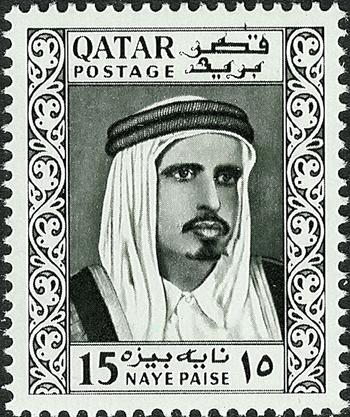
\includegraphics[width=0.3\textwidth]{./graphics/qatar.jpg}
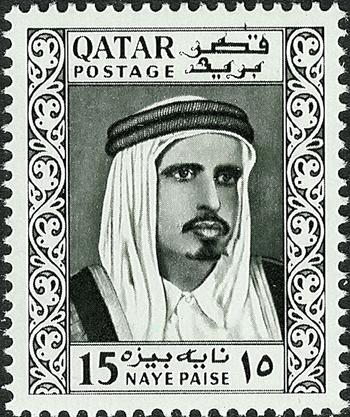
\includegraphics[width=0.3\textwidth]{./graphics/qatar.jpg}
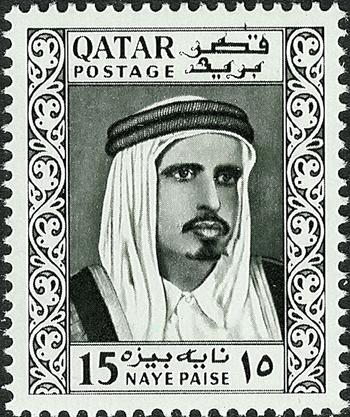
\includegraphics[width=0.3\textwidth]{./graphics/qatar.jpg}
\parbox[t]{3.3cm}{\small\hangindent.1em \textsc{\textbf{SG 1}}  This is a test with the heir apparent portrait.} \parbox[t]{3.3cm}{\textsc{sg 2} \small This is a test with the heir apparent portrait.}\parbox[t]{3.3cm}{\textsc{sg 3} \small This is a test with the heir apparent portrait. This is another test fr something else.}


\vspace{4pt}
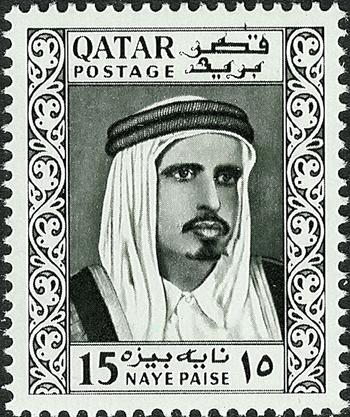
\includegraphics[width=0.3\textwidth]{./graphics/qatar.jpg}
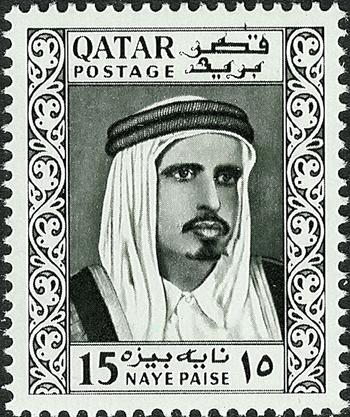
\includegraphics[width=0.3\textwidth]{./graphics/qatar.jpg}

\parbox[t]{3.3cm}{\small\hangindent.1em \textsc{\textbf{SG 4}}  This is a test with the heir apparent portrait.} \parbox[t]{3.3cm}{\textsc{sg 5} \small This is a test with the heir apparent portrait.}

\caption{Stamps with the portrait of Sheikh Ali AL Thani were printed in Britain by De La Rue Security Printers. The sheikh Ahmed Bin Abdullah stamps were printed with the same design as the Sheikh Ali al Thani stamps.}
\end{figure}
\lipsum[2]

\chapter{Appendix A Logic on pictures}
\section{Countries}
Countries are manipulated via the countries package.
The countries list is used extensively to add prefix commands, create indices and the like.

The master table is called \texttt{countries.dat}.

Secondary tables are \texttt{countrycategories.dat}


If set $<5$ layout straight

If set 5  layout 3 and 2

If set 6 layout 3 3

If set 7 layout 2 3 2

%% Determine the scaling factor by placing the first three images in a row.
%% First test the natural size of the images if they are smaller than
%% textwidth, we do not want to scale up as they might not look so nice

\newcounter{ct}
\outer\long\def\Typesetter#1#2#3{%
%% #1 first row
%% #2 number of rows in between
%% #3 last row
\newbox\imagetestbox
\newbox\rowi
\newbox\rowii
\newbox\rowiii
\newbox\rowiv
\newbox\rowv
\newbox\rowvi
\sbox \imagetestbox{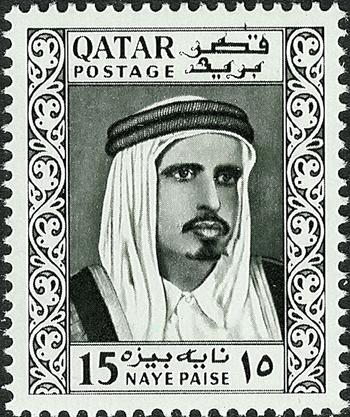
\includegraphics{./graphics/qatar.jpg}
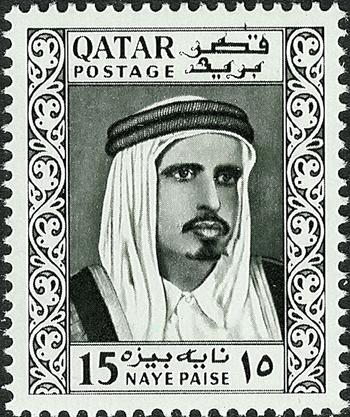
\includegraphics{./graphics/qatar.jpg}
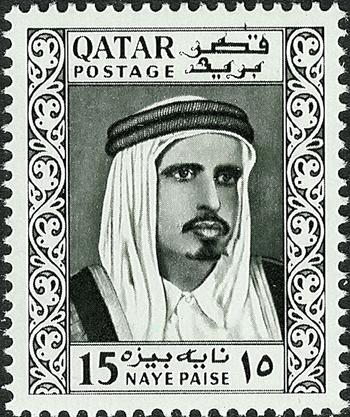
\includegraphics{./graphics/qatar.jpg}} 

\def\naturaltextwidth{\number\textwidth}
\def\naturalimagewidth{\number\wd\imagetestbox}

%\number\wd\imagetestbox
%
%\number\textwidth
%
%%\ifdim\naturaltextwidth<\naturalimagewidth We need to scale \else smaller \fi

\FPdiv\ascale{\naturaltextwidth}{\naturalimagewidth}
\FPround\ascale{\ascale}{2}
%\ascale

\sbox\rowiii{%
\includegraphics[width=\ascale\textwidth]{./graphics/22.jpg}
\includegraphics[width=\ascale\textwidth]{./graphics/23.jpg}
\includegraphics[width=\ascale\textwidth]{./graphics/24.jpg}
}


\sbox \rowii{%
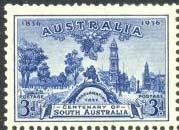
\includegraphics[width=\ascale\textwidth]{./graphics/SG162.jpg}
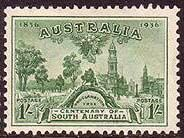
\includegraphics[width=\ascale\textwidth]{./graphics/SG163.jpg}
}

\def\Rowi##1{%
  \sbox \rowi{%
  \includegraphics[width=\ascale\textwidth]{##1}}
  \usebox\rowi
}


%% This will have to be changed to a macro which is long and outer
\begin{figure}[hp]
\begin{center}
%% we first determine the first row, and fetch the image names
\ifnum#1=1 \Rowi{./graphics/martin-schoeller/angelina_jolie_2004}
\else

  \ifnum#1=2 \usebox\rowii\fi
\fi
%% loop for the rows in between

\setcounter{ct}{0}
\loop
\ifnum\thect<#2
  \usebox\rowiii 
  \stepcounter{ct}
  image
\repeat

%% we now get the last
\ifnum#3=2\usebox\rowii\fi
\end{center}
\caption{(#1+#2x3+#3) images}
\end{figure}
}%end Typesetter macro





%% Example
%% If you examine the patterns, the first and last row changes
%% If mod 3 = 1 first and last row are 2 images each (7,10 images etc)
%% If mod 3 = 2 last row is 2 images
%% If mod 3 = 0 first row three last row three (6,9,12 images etc)
%% This is only true for equal images

\makeatletter
%% Holds number of images in first row
\newcounter{firstrow} \setcounter{firstrow}{0}
%% Holds number of images in last row
\newcounter{lastrow} \setcounter{lastrow}{0}
%% Holds the total images in first + last row
\newcounter{nrows} \setcounter{nrows}{0}

\newcounter{numberrows} \setcounter{numberrows}{0}
\def\get@pattern#1#2{%

\gdef\Modulus{\intcalcMod{#1}{#2}}

\ifnum#1>2
\ifnum\Modulus=1 \setcounter{nrows}{4}
      \setcounter{firstrow}{2}\setcounter{lastrow}{2}
      \setcounter{numberrows}{\number\numexpr((#1-4)/#2)}
      \gdef\number@full@rows{\thenumberrows}
  \else
     \ifnum\Modulus=2\setcounter{nrows}{2}
       \setcounter{firstrow}{0}\setcounter{lastrow}{2}
       \setcounter{numberrows}{\number\numexpr((#1-2)/#2)}
       \gdef\number@full@rows{\thenumberrows}
     \else
       \ifnum\Modulus=0%OK 
         \setcounter{firstrow}{0}\setcounter{lastrow}{0}
          \gdef\balance{#1}
          \gdef\number@full@rows{\intcalcDiv{\balance}{#2}}
       \fi
    \fi
  \fi
\else
   \setcounter{firstrow}{#1}\setcounter{lastrow}{0}\setcounter{nrows}{0}
   \gdef\number@full@rows{0}
\fi

%\if@first First are two \else 0 images \fi
%\if@last Last are two \else 0 images \fi
%
%
%%% We need to determine the balance of the images
%% #1-\the\nrows
}





\makeatletter
%% Add some more Australian Sets
%SG1-8
\addset{Australia}{SG1-SG8}{opening of Parliament House\footnotemark, Canberra\footnotetext{test}}{1927}{KGV}
\setlist{Australia}{SG1-SG8}{1,2,3,4,5,6,8}
\addstamp{Australia}{SG1}{Australia\footnotemark SG 105 11/2d brownish lake, no watermark, perf 11}{1 1/1d}{australia/SG1}{}{}{}{}
\addstamp{Australia}{SG2}{Australia SG 105 11/2d brownish lake, no watermark, perf 11}{1 1/1d}{australia/SG2}{}{}{}{}
\addstamp{Australia}{SG3}{Australia SG 105 11/2d brownish lake, no watermark, perf 11}{1 1/1d}{australia/SG3}{}{}{}{}
\addstamp{Australia}{SG4}{Australia SG 105 11/2d brownish lake, no watermark, perf 11}{1 1/1d}{australia/SG4}{}{}{}{}
\addstamp{Australia}{SG5}{Australia SG 105 11/2d brownish lake, no watermark, perf 11}{1 1/1d}{australia/SG5}{}{}{}{}
\addstamp{Australia}{SG6}{Australia SG 105 11/2d brownish lake, no watermark, perf 11}{1 1/1d}{australia/SG6}{}{}{}{}
%\addstamp{Australia}{SG7}{Australia SG 105 11/2d brownish lake, no watermark, perf 11}{1 1/1d}{australia/SG7}{}{}{}{}
\addstamp{Australia}{SG8}{Australia SG 105 11/2d brownish lake, no watermark, perf 11}{1 1/1d}{australia/SG8}{}{}{}{}

%SG1-8
\addset{Australia}{SG9-SG13}{opening of Parliament House, Canberra}{1927}{KGV}
\setlist{Australia}{SG9-SG13}{9,10,11,13}
\addstamp{Australia}{SG9}{Australia SG 105 11/2d brownish lake, no watermark, perf 11}{1 1/1d}{australia/SG9}{}{}{}{}
\addstamp{Australia}{SG10}{Australia SG 105 11/2d brownish lake, no watermark, perf 11}{1 1/1d}{australia/SG10}{}{}{}{}
\addstamp{Australia}{SG11}{Australia SG 105 11/2d brownish lake, no watermark, perf 11}{1 1/1d}{australia/SG11}{}{}{}{}
%\addstamp{Australia}{SG12}{Australia SG 105 11/2d brownish lake, no watermark, perf 11}{1 1/1d}{australia/SG12}{}{}{}{}
\addstamp{Australia}{SG13}{Australia SG 105 11/2d brownish lake, no watermark, perf 11}{1 1/1d}{australia/SG13}{}{}{}{}
\addstamp{Australia}{SG14}{Australia SG 105 11/2d brownish lake, no watermark, perf 11}{1 1/1d}{australia/SG14}{}{}{}{}

%SG15-16
\addset{Australia}{SG15-SG16}{opening of Parliament House, Canberra}{1927}{KGV}
\setlist{Australia}{SG15-SG16}{16}
\addstamp{Australia}{SG15}{Australia SG 105 11/2d brownish lake, no watermark, perf 11}{1 1/1d}{australia/SG15}{}{}{}{}
\addstamp{Australia}{SG16}{Australia SG 105 11/2d brownish lake, no watermark, perf 11}{1 1/1d}{australia/SG16}{}{}{}{}

%SG17
\addset{Australia}{SG17-SG17}{opening of Parliament House, Canberra}{1927}{KGV}
\setlist{Australia}{SG17-SG17}{17}
\addstamp{Australia}{SG17}{Australia SG 105 11/2d brownish lake, no watermark, perf 11}{1 1/1d}{australia/SG15}{}{}{}{}

%SG19
\addset{Australia}{SG19-SG19}{opening of Parliament House, Canberra}{1927}{KGV}
\setlist{Australia}{SG19-SG19}{19}
\addstamp{Australia}{SG19}{Australia SG 105 11/2d brownish lake, no watermark, perf 11}{1 1/1d}{australia/SG15}{}{}{}{}
 
%SG20-23
\addset{Australia}{SG20-SG23}{opening of Parliament House, Canberra}{1927}{KGV}
\setlist{Australia}{SG20-SG23}{20,21,22,23}
\addstamp{Australia}{SG20}{Australia SG 105 11/2d brownish lake, no watermark, perf 11}{1 1/1d}{australia/SG20}{}{}{}{}
\addstamp{Australia}{SG21}{Australia SG 105 11/2d brownish lake, no watermark, perf 11}{1 1/1d}{australia/SG21}{}{}{}{}
\addstamp{Australia}{SG22}{Australia SG 105 11/2d brownish lake, no watermark, perf 11}{1 1/1d}{australia/SG22}{}{}{}{}
\addstamp{Australia}{SG23}{Australia SG 105 11/2d brownish lake, no watermark, perf 11}{1 1/1d}{australia/SG23}{}{}{}{}


%SG20-23
\addset{Australia}{SG24-SG30}{opening of Parliament House, Canberra}{1927}{KGV}
\setlist{Australia}{SG24-SG30}{24,25,26,27,28,29,30}
\addstamp{Australia}{SG24}{Australia SG 105 11/2d brownish lake, no watermark, perf 11}{1 1/1d}{australia/SG24}{}{}{}{}
\addstamp{Australia}{SG25}{Australia SG 105 11/2d brownish lake, no watermark, perf 11}{1 1/1d}{australia/SG25}{}{}{}{}
\addstamp{Australia}{SG26}{Australia SG 105 11/2d brownish lake, no watermark, perf 11}{1 1/1d}{australia/SG26}{}{}{}{}
\addstamp{Australia}{SG27}{Australia SG 105 11/2d brownish lake, no watermark, perf 11}{1 1/1d}{australia/SG27}{}{}{}{}
\addstamp{Australia}{SG28}{Australia SG 105 11/2d brownish lake, no watermark, perf 11}{1 1/1d}{australia/SG28}{}{}{}{}
\addstamp{Australia}{SG29}{Australia SG 105 11/2d brownish lake, no watermark, perf 11}{1 1/1d}{australia/SG29}{}{}{}{}
\addstamp{Australia}{SG30}{Australia SG 105 11/2d brownish lake, no watermark, perf 11}{1 1/1d}{australia/SG30}{}{}{}{}


%36-43
\addset{Australia}{SG36-SG43}{opening of Parliament House, Canberra}{1927}{KGV}
\setlist{Australia}{SG36-SG43}{36,37,38,39,40,41,42,43,44}
\addstamp{Australia}{SG36}{Australia SG 105 11/2d brownish lake, no watermark, perf 11}{1 1/1d}{australia/SG36}{}{}{}{}
\addstamp{Australia}{SG37}{Australia SG 105 11/2d brownish lake, no watermark, perf 11}{1 1/1d}{australia/SG37}{}{}{}{}
\addstamp{Australia}{SG38}{Australia SG 105 11/2d brownish lake, no watermark, perf 11}{1 1/1d}{australia/SG38}{}{}{}{}
\addstamp{Australia}{SG39}{Australia SG 105 11/2d brownish lake, no watermark, perf 11}{1 1/1d}{australia/SG39}{}{}{}{}
\addstamp{Australia}{SG40}{Australia SG 105 11/2d brownish lake, no watermark, perf 11}{1 1/1d}{australia/SG40}{}{}{}{}
\addstamp{Australia}{SG41}{Australia SG 105 11/2d brownish lake, no watermark, perf 11}{1 1/1d}{australia/SG41}{}{}{}{}
\addstamp{Australia}{SG42}{Australia SG 105 11/2d brownish lake, no watermark, perf 11}{1 1/1d}{australia/SG42}{}{}{}{}
\addstamp{Australia}{SG43}{Australia SG 105 11/2d brownish lake, no watermark, perf 11}{1 1/1d}{australia/SG43}{}{}{}{}
\addstamp{Australia}{SG44}{Australia SG 105 11/2d brownish lake, no watermark, perf 11 \pounds 1800}{1 1/1d}{australia/SG44a}{}{}{}{}

\addset{Australia}{SG45-SG45}{opening of Parliament House, Canberra}{1927}{KGV}
\setlist{Australia}{SG45-SG45}{45,45}
\addstamp{Australia}{SG45}{Australia SG 105 11/2d brownish lake, no watermark, perf 11 \pounds 1800}{1 1/1d}{australia/SG45}{}{}{}{}

\addset{Australia}{SG47-SG59}{opening of Parliament House, Canberra}{1927}{KGV}
\setlist{Australia}{SG47-SG59}{47,48,49,50,51,53,57,58,59}
%\addstamp{Australia}{SG46}{Australia SG 105 11/2d brownish lake, no watermark, perf 11 \pounds 1800}{1 1/1d}{australia/SG46}{}{}{}{}
\addstamp{Australia}{SG47}{Australia SG 105 11/2d brownish lake, no watermark, perf 11 \pounds 1800}{1 1/1d}{australia/SG47}{}{}{}{}
\addstamp{Australia}{SG48}{Australia SG 105 11/2d brownish lake, no watermark, perf 11 \pounds 1800}{1 1/1d}{australia/SG48}{}{}{}{}
\addstamp{Australia}{SG49}{Australia SG 105 11/2d brownish lake, no watermark, perf 11 \pounds 1800}{1 1/1d}{australia/SG49}{}{}{}{}
\addstamp{Australia}{SG50}{Australia SG 105 11/2d brownish lake, no watermark, perf 11 \pounds 1800}{1 1/1d}{australia/SG50}{}{}{}{}
\addstamp{Australia}{SG51}{Australia SG 105 11/2d brownish lake, no watermark, perf 11 \pounds 1800}{1 1/1d}{australia/SG51}{}{}{}{}
\addstamp{Australia}{SG53}{Australia SG 105 11/2d brownish lake, no watermark, perf 11 \pounds 1800}{1 1/1d}{australia/SG53}{}{}{}{}
\addstamp{Australia}{SG57}{Australia SG 105 11/2d brownish lake, no watermark, perf 11 \pounds 1800}{1 1/1d}{australia/SG58}{}{}{}{}
\addstamp{Australia}{SG58}{Australia SG 105 11/2d brownish lake, no watermark, perf 11 \pounds 1800}{1 1/1d}{australia/SG58}{}{}{}{}
\addstamp{Australia}{SG59}{Australia SG 105 11/2d brownish lake, no watermark, perf 11 \pounds 1800}{1 1/1d}{australia/SG59}{}{}{}{}

\addset{Australia}{SG60-SG66}{opening of Parliament House, Canberra}{1927}{KGV}
\setlist{Australia}{SG60-SG66}{60,61,62,63,64,65,66}
%\addstamp{Australia}{SG46}{Australia SG 105 11/2d brownish lake, no watermark, perf 11 \pounds 1800}{1 1/1d}{australia/SG46}{}{}{}{}
\addstamp{Australia}{SG60}{Australia SG 105 11/2d brownish lake, no watermark, perf 11 \pounds 1800}{1 1/1d}{australia/SG60}{}{}{}{}
\addstamp{Australia}{SG61}{Australia SG 105 11/2d brownish lake, no watermark, perf 11 \pounds 1800}{1 1/1d}{australia/SG61}{}{}{}{}
\addstamp{Australia}{SG62}{Australia SG 105 11/2d brownish lake, no watermark, perf 11 \pounds 1800}{1 1/1d}{australia/SG62}{}{}{}{}
\addstamp{Australia}{SG63}{Australia SG 105 11/2d brownish lake, no watermark, perf 11 \pounds 1800}{1 1/1d}{australia/SG63}{}{}{}{}
\addstamp{Australia}{SG64}{Australia SG 105 11/2d brownish lake, no watermark, perf 11 \pounds 1800}{1 1/1d}{australia/SG64}{}{}{}{}
\addstamp{Australia}{SG65}{Australia SG 105 11/2d brownish lake, no watermark, perf 11 \pounds 1800}{1 1/1d}{australia/SG65}{}{}{}{}
\addstamp{Australia}{SG66}{Australia SG 105 11/2d brownish lake, no watermark, perf 11 \pounds 1800}{1 1/1d}{australia/SG66}{}{}{}{}

\addset{Australia}{SG73-SG75}{Die II \& Die IIb 1st May 1924}{1927}{KGV}
\setlist{Australia}{SG73-SG75}{73,74,75}
\addstamp{Australia}{SG73}{Australia SG 74 2/- Maroon (Die II) (1.5.24) watermark 6, perf 12. Printed by Harrison to February 1926, Mullett till June 1927, Ash thereafter \pounds 1800}{1 1/1d}{australia/SG73}{}{}{}{}
\addstamp{Australia}{SG74}{Australia SG 105 11/2d brownish lake, no watermark, perf 11 \pounds 1800}{1 1/1d}{australia/SG74}{}{}{}{}
\addstamp{Australia}{SG75}{Australia SG 75 1 Grey (Die IIB) (1.5.24) watermark 6 perf 12}{}{australia/SG75}{}{}{}{}


\addset{Australia}{SG76-SG85}{opening of Parliament House, Canberra}{1927}{KGV}
\setlist{Australia}{SG76-SG85}{76,77,78,79,80,81,82,83,84}
\addstamp{Australia}{SG76}{Australia SG 105 11/2d brownish lake, no watermark, perf 11}{1 1/1d}{australia/SG76}{}{}{}{}
\addstamp{Australia}{SG77}{Australia SG 105 11/2d brownish lake, no watermark, perf 11}{1 1/1d}{australia/SG77}{}{}{}{}
\addstamp{Australia}{SG78}{Australia SG 105 11/2d brownish lake, no watermark, perf 11}{1 1/1d}{australia/SG78}{}{}{}{}
\addstamp{Australia}{SG79}{Australia SG 105 11/2d brownish lake, no watermark, perf 11}{1 1/1d}{australia/SG79}{}{}{}{}
\addstamp{Australia}{SG80}{Australia SG 105 11/2d brownish lake, no watermark, perf 11}{1 1/1d}{australia/SG80}{}{}{}{}
\addstamp{Australia}{SG81}{Australia SG 105 11/2d brownish lake, no watermark, perf 11}{1 1/1d}{australia/SG81}{}{}{}{}
\addstamp{Australia}{SG82}{Australia SG 105 11/2d brownish lake, no watermark, perf 11}{1 1/1d}{australia/SG82}{}{}{}{}
\addstamp{Australia}{SG83}{Australia SG 105 11/2d brownish lake, no watermark, perf 11}{1 1/1d}{australia/SG83}{}{}{}{}
\addstamp{Australia}{SG84}{Australia SG 105 11/2d brownish lake, no watermark, perf 11}{1 1/1d}{australia/SG84}{}{}{}{}
\addstamp{Australia}{SG85}{Australia SG 105 11/2d brownish lake, no watermark, perf 11}{1 1/1d}{australia/SG85}{}{}{}{}


\addset{Australia}{SG86-SG95}{opening of Parliament House, Canberra}{1927}{KGV}
\setlist{Australia}{SG86-SG95}{87,89,90,91,92,93,94,95,96}
\addstamp{Australia}{SG86}{Australia SG 105 11/2d brownish lake, no watermark, perf 11}{1 1/1d}{australia/SG86}{}{}{}{}
\addstamp{Australia}{SG87}{Australia SG 105 11/2d brownish lake, no watermark, perf 11}{1 1/1d}{australia/SG87}{}{}{}{}
%\addstamp{Australia}{SG88}{Australia SG 105 11/2d brownish lake, no watermark, perf 11}{1 1/1d}{australia/SG88}{}{}{}{}
\addstamp{Australia}{SG89}{Australia SG 105 11/2d brownish lake, no watermark, perf 11}{1 1/1d}{australia/SG89}{}{}{}{}
\addstamp{Australia}{SG90}{Australia SG 105 11/2d brownish lake, no watermark, perf 11}{1 1/1d}{australia/SG90}{}{}{}{}
\addstamp{Australia}{SG91}{Australia SG 105 11/2d brownish lake, no watermark, perf 11}{1 1/1d}{australia/SG91}{}{}{}{}
\addstamp{Australia}{SG92}{Australia SG 105 11/2d brownish lake, no watermark, perf 11}{1 1/1d}{australia/SG92}{}{}{}{}
\addstamp{Australia}{SG93}{Australia SG 105 11/2d brownish lake, no watermark, perf 11}{1 1/1d}{australia/SG93}{}{}{}{}
\addstamp{Australia}{SG94}{Australia SG 105 11/2d brownish lake, no watermark, perf 11}{1 1/1d}{australia/SG94}{}{}{}{}
\addstamp{Australia}{SG95}{Australia SG 105 11/2d brownish lake, no watermark, perf 11}{1 1/1d}{australia/SG95}{}{}{}{}


\addset{Australia}{SG96-SG103}{opening of Parliament House, Canberra}{1927}{KGV}
\setlist{Australia}{SG96-SG103}{96,97,98,99,100,101,102,103,104}
\addstamp{Australia}{SG96}{Australia SG 105 11/2d brownish lake, no watermark, perf 11}{1 1/1d}{australia/SG96}{}{}{}{}
\addstamp{Australia}{SG97}{Australia SG 105 11/2d brownish lake, no watermark, perf 11}{1 1/1d}{australia/SG97}{}{}{}{}
\addstamp{Australia}{SG98}{Australia SG 105 11/2d brownish lake, no watermark, perf 11}{1 1/1d}{australia/SG98}{}{}{}{}
\addstamp{Australia}{SG99}{Australia SG 105 11/2d brownish lake, no watermark, perf 11}{1 1/1d}{australia/SG99}{}{}{}{}
\addstamp{Australia}{SG100}{Australia SG 105 11/2d brownish lake, no watermark, perf 11}{1 1/1d}{australia/SG100}{}{}{}{}
\addstamp{Australia}{SG101}{Australia SG 105 11/2d brownish lake, no watermark, perf 11}{1 1/1d}{australia/SG101}{}{}{}{}
\addstamp{Australia}{SG102}{Australia SG 105 11/2d brownish lake, no watermark, perf 11}{1 1/1d}{australia/SG102}{}{}{}{}
\addstamp{Australia}{SG103}{Australia SG 105 11/2d brownish lake, no watermark, perf 11}{1 1/1d}{australia/SG103}{}{}{}{}
\addstamp{Australia}{SG104}{Australia SG 105 11/2d brownish lake, no watermark, perf 11}{1 1/1d}{australia/SG104}{}{}{}{}



%SG105
\addset{Australia}{SG105-SG105}{opening of Parliament House, Canberra}{1927}{KGV}
\setlist{Australia}{SG105-SG105}{105}
\addstamp{Australia}{SG105}{Australia SG 105 11/2d brownish lake, no watermark, perf 11}{1 1/1d}{australia/SG105}{}{}{}{}

\addset{Australia}{SG106-SG106}{opening of Parliament House, Canberra}{1927}{KGV}
\setlist{Australia}{SG106-SG106}{106}
\addstamp{Australia}{SG106}{Australia SG 105 11/2d brownish lake, no watermark, perf 11}{1 1/1d}{australia/SG106}{}{}{}{}

\addset{Australia}{SG107-SG114}{opening of Parliament House, Canberra}{1927}{KGV}
\setlist{Australia}{SG107-SG114}{107,108,109,110,111,112,114}
%\addstamp{Australia}{SG106}{Australia SG 105 11/2d brownish lake, no watermark, perf 11}{1 1/1d}{australia/SG106}{}{}{}{}
\addstamp{Australia}{SG107}{Australia SG 105 11/2d brownish lake, no watermark, perf 11}{1 1/1d}{australia/SG107}{}{}{}{}
\addstamp{Australia}{SG108}{Australia SG 105 11/2d brownish lake, no watermark, perf 11}{1 1/1d}{australia/SG108}{}{}{}{}
\addstamp{Australia}{SG109}{Australia SG 105 11/2d brownish lake, no watermark, perf 11}{1 1/1d}{australia/SG109}{}{}{}{}
\addstamp{Australia}{SG110}{Australia SG 105 11/2d brownish lake, no watermark, perf 11}{1 1/1d}{australia/SG110}{}{}{}{}
\addstamp{Australia}{SG111}{Australia SG 105 11/2d brownish lake, no watermark, perf 11}{1 1/1d}{australia/SG111}{}{}{}{}
\addstamp{Australia}{SG112}{Australia SG 105 11/2d brownish lake, no watermark, perf 11}{1 1/1d}{australia/SG112}{}{}{}{}
\addstamp{Australia}{SG113}{Australia SG 105 11/2d brownish lake, no watermark, perf 11}{1 1/1d}{australia/SG113}{}{}{}{}
\addstamp{Australia}{SG114}{Australia SG 105 11/2d brownish lake, no watermark, perf 11}{1 1/1d}{australia/SG114}{}{}{}{}




%SG115 First Air mail issue
\addset{Australia}{SG115-SG115}{First Air Mail Issue}{1929}{KGV}
\setlist{Australia}{SG115-SG115}{115}
\addstamp{Australia}{SG115}{Australia SG 115 3d green (shades) DH66 biplane and pastoral scene, airmail, no watermark, perf 11
}{3d}{australia/SG115}{CCC}{BBB}{AAA}{Designer: R.A. Harrison in conjunction with Harold Herbert - Engraver: A. Taylor - Printer: John Ash
Issued 20 May without Watermark with perforation 11
The design is of a De Haviland biplane, flying over a flock of Merino sheep with stands of eucalypts on 
either side, issued for the  Perth-Adelaide air service, inaugurated 2 June, 1929, the stamp was released 
in two types; Type A, the mesh of the stamp is vertical with a stamp size of 31 x 22 mm, while Type B, the 
mesh of the stamp is horizontal with a stamp size of 31.75  x 21.5 mm, a 36d Booklet was also released, 
an Official stamp punctured OS was also issued for Government use, this stamp could be in either type A 
or B.}

%SG116 Centenary of Western Australia
\addset{Australia}{SG116-SG116}{Centenary of Western Australia}{1929}{KGV}
\setlist{Australia}{SG116-SG116}{116}
\addstamp{Australia}{SG116}{Australia SG 116 11/2d dull scarlet Centenary of Western Australia, Black Swan, no watermark, perf 11
Also, 
SG 116a Re-entry (``T'' of ``AUSTRALIA'' clearly double)
}{3d}{australia/SG116}{}{}{}{Designer: G. Pitt-Morrison - Engraver: Frank D. Manley - Printer: John Ash
Issued 28 September without Watermark with perforation 11
This stamp was released to commemorate the 100th Anniversary of the founding of Western Australia, 
the design incorporates a Swan as the central figure, with Kangaroo Paws (W. A. State Flower) \& 
Eucalyptus flowers \& leaves, an Official stamp punctured OS was also issued for Government use. }




%117
\addset{Australia}{SG117-SG118}{Charles Sturt, Centenary}{1927}{KGV}
\setlist{Australia}{SG117-SG118}{117,118}
\addstamp{Australia}{SG117}{Australia SG 117 1 1/2d scarlet Centenary of exploration of Murray River by Captain Charles Sturt, no watermark, perf 11.}{1 1/1d}{australia/SG117}{}{}{}{}
\addstamp{Australia}{SG118}{Australia SG 118 3d blue, Centenary of exploration of Murray River by Captain Charles Sturt, no watermark, perf 11.}{3d}{australia/SG118}{}{}{}{Designer: R.A. Harrison - Engraver: Frank D. Manley - Printer: John Ash
Issued 2 June without Watermark with perforation 11. \\
This release commemorates the 100th anniversary of Captain John Sturt's voyage of discovery along the 
lower Murray River, the design shows a portrait of Captain Sturt taken from a painting that hangs in the 
Adelaide Art Gallery, also a large Aboriginal shield, a smaller shield (called a coolamon) two spear heads 
and the tail feathers of a lyre bird.}

%119-120
\addset{Australia}{SG119-SG120}{Two pence and five pence overprint}{1927}{KGV}
\setlist{Australia}{SG119-SG120}{119,120}
\addstamp{Australia}{SG119}{2d on 1½d golden scarlet, watermark 7, perf 13½ x 12½}{1 1/1d}{australia/SG119}{}{}{}{}
\addstamp{Australia}{SG120}{Australia SG 120 5d on 4½d violet, watermark 7, perf 13½ x 12½}{1 1/1d}{australia/SG120}{}{}{}{}


%121-123
\addset{Australia}{SG121-SG123}{Two pence and five pence overprint}{1927}{KGV}
\setlist{Australia}{SG121-SG123}{121,122,123}
\addstamp{Australia}{SG121}{2d on 1½d golden scarlet, watermark 7, perf 13½ x 12½}{1 1/1d}{australia/SG121}{}{}{}{}
\addstamp{Australia}{SG122}{Australia SG 120 5d on 4½d violet, watermark 7, perf 13½ x 12½}{1 1/1d}{australia/SG122}{}{}{}{}
\addstamp{Australia}{SG123}{Australia SG 120 5d on 4½d violet, watermark 7, perf 13½ x 12½}{1 1/1d}{australia/SG123}{}{}{}{}


%124-131 King George Definitives
\addset{Australia}{SG124-SG131}{King George Definitives}{1931}{KGV}
\setlist{Australia}{SG124-SG131}{124,125,126,127,128,129,130,131}

\addstamp{Australia}{SG124}{Australia SG 124 1/2d orange (2.33) watermark 15, perf 131/2 x 12 1/2}{australia/SG124}{}{}{}{}{}

\addstamp{Australia}{SG125}{Australia SG 125 1d green (Die I) (10.31), watermark 15, perf 131/2 x 121/2}{australia/SG125}{}{}{}{}{}

\addstamp{Australia}{SG126}{Australia SG 126 11/2d red-brown (10.36), watermark 15,}{1 1/2d}{australia/SG126}{}{}{}{}{}

\addstamp{Australia}{SG127}{Australia SG 127 2d golden scarlet (Die III) (18.12.31), watermark 15, perf 131/2 x 121/2}{1 1/2d}{australia/SG127}{}{}{}{}
\addstamp{Australia}{SG128}{green (1.12.42) Queen Elizabeth. Watermark 15, perf 15 x 14}{1 1/2d}{australia/SG128}{Australia SG 128 3d ultramarine (Die II) (30.9.32), watermark 15}{}{}{}
\addstamp{Australia}{SG129}{Australia SG 129 4d yellow-olive (2.33), watermark 15}{1 1/2d}{australia/SG129}{}{}{}{}
\addstamp{Australia}{SG130}{green (1.12.42) Queen Elizabeth. Watermark 15, perf 15 x 14}{1 1/2d}{australia/SG130}{Australia SG 130 5d orange-brown (Die II) (25.2.32), watermark 15}{}{}{}
\addstamp{Australia}{SG131}{Australia SG 131 1/4 turquoise (18.8.32), watermark 15}{1 1/2d}{australia/SG131}{}{}{}{}

%132-138
\addset{Australia}{SG132-SG138}{Roos}{1931}{KGV}
\setlist{Australia}{SG132-SG138}{132,133,134,135,136,137,138}
\addstamp{Australia}{SG132}{Australia SG 132 6d chestnut (Die IIB) (20.4.32) watermark 15, perf 12}{}{australia/SG132}{}{}{}{}

\addstamp{Australia}{SG133}{Australia SG 138 1/4 turquoise (18.8.32), watermark 15}{TESTUINGGG}{australia/SG133}{a}{a}{a}{aaaaa}

\addstamp{Australia}{SG134}{Australia SG 134 1/4 turquoise (18.8.32), watermark 15}{1 1/2d}{australia/SG134}{}{}{}{}
\addstamp{Australia}{SG135}{Australia SG 135 1/4 turquoise (18.8.32), watermark 15}{1 1/2d}{australia/SG135}{}{}{}{}
\addstamp{Australia}{SG136}{Australia SG 136 1/4 turquoise (18.8.32), watermark 15}{1 1/2d}{australia/SG136}{}{}{}{}
\addstamp{Australia}{SG137}{Australia SG 137 1/4 turquoise (18.8.32), watermark 15}{1 1/2d}{australia/SG137}{}{}{}{}
\addstamp{Australia}{SG138}{Australia SG 138 1/4 turquoise (18.8.32), watermark 15}{1 1/2d}{australia/SG138}{}{}{}{}

%140-140a

\addset{Australia}{SG140-140a}{Lyrebird}{1933}{KGVI}
\setlist{Australia}{SG140-SG140a}{140,140a}
\addstamp{Australia}{SG140}{Australia SG 140 2d scarlet, Sydney Harbour Bridge. Recess printed, no watermark, perf 11.}{3d}{australia/SG140}{}{}{}{}
\addstamp{Australia}{SG140a}{Australia SG 141 2d scarlet, Sydney Harbour Bridge. Recess printed, no watermark, perf 11.}{3d}{australia/SG140a}{}{}{}{}


%141-144 
\addset{Australia}{SG141-SG144}{Sydney Harbour Bridge}{1934}{KGVI}
\setlist{Australia}{SG141-SG144}{141,142,143,144}
\addstamp{Australia}{SG141}{Australia SG 141 2d scarlet, Sydney Harbour Bridge. Recess printed, no watermark, perf 11.}{3d}{australia/SG141}{}{}{}{}

\addstamp{Australia}{SG142}{Australia SG 142 2d blue, Sydney Harbour Bridge. Recess printed, no watermark, perf 11.}{3d}{australia/SG142}{}{}{}{}

\addstamp{Australia}{SG143}{Australia SG 143 5/- blue-green, Sydney Harbour Bridge. Recess printed, no watermark, perf 11.}{3d}{australia/SG143}{}{}{}{}

\addstamp{Australia}{SG144}{Australia SG 144 2d scarlet, Sydney Harbour Bridge. Typographically printed, watermark 15, perf 101/2. Note:
Stamps as SG 144 without watermark and perf 11 are forgeries made in 1932 to defraud the P.O.}{3d}{australia/SG144}{}{}{}{}

%146
\addset{Australia}{SG146-SG146}{Laughing Kookaburra}{1934}{KGVI}
\setlist{Australia}{SG146-SG146}{146}
\addstamp{Australia}{SG146}{Australia SG 146 6d red-brown, Laughing Kookaburra. Watermark 15, perf 131/2 x 121/2.}{3d}{australia/SG146}{}{}{}{}




%147
\addset{Australia}{SG147-SG149}{Centenary of Victoria}{1934}{KGVI}
\setlist{Australia}{SG147-SG149}{147,148,149}
\addstamp{Australia}{SG147}{Australia SG 118 3d blue, Centenary of exploration of Murray River by Captain Charles Sturt, no watermark, perf 11.}{3d}{australia/SG147}{}{}{}{}
\addstamp{Australia}{SG148}{Australia SG 118 3d blue, Centenary of exploration of Murray River by Captain Charles Sturt, no watermark, perf 11.}{3d}{australia/SG148}{}{}{}{}
\addstamp{Australia}{SG149}{Australia SG 149 1/- black, Centenary of Victoria, Melbourne and River Yarra. Watermark 15, perf 101/2. Also SG 149a perf 111/2}{3d}{australia/SG149}{}{}{}{}



%SG193-SG195
\addset{Australia}{SG193-SG195}{The Foundation of New South Wales}{1938}{KGVI}
\setlist{Australia}{SG193-SG195}{193,194,195}
\addstamp{Australia}{SG193}{deep ultramarine\footnote{Shades of ultramarine exist.}. 30th anniversary of first air crossing of Tasman Sea, Sir Charles Kingsford Smith and Southern Cross.}{1 1/1d}{australia/SG193}{}{}{}{}
\addstamp{Australia}{SG194}{deep ultramarine. 30th anniversary of first air crossing of Tasman Sea, Sir Charles Kingsford Smith and Southern Cross.}{1 1/1d}{australia/SG194}{}{}{}{}
\addstamp{Australia}{SG195}{deep ultramarine. 30th anniversary of first air crossing of Tasman Sea, Sir Charles Kingsford Smith and Southern Cross.}{1 1/1d}{australia/SG195}{}{}{}{}


%SG196-SG199
\addset{Australia}{SG196-SG199}{Australian Imperial Forces}{1940}{KGVI}
\setlist{Australia}{SG196-SG199}{196,197,198,199}
\addstamp{Australia}{SG196}{July 15th, 1940 Australia SG 196 1d green. Australian Imperial Forces and Nurse. Watermark 15 sideways, perf 14 x 13 1/2}{1 1/1d}{australia/SG196}{}{}{}{}
\addstamp{Australia}{SG197}{Australia SG 197 scarlet. Australian Imperial Forces and Nurse. Watermark 15 sideways, perf 14 x 13}{1 1/1d}{australia/SG197}{}{}{}{}
\addstamp{Australia}{SG198}{Australia SG 198 3d blue. Australian Imperial Forces and Nurse. Watermark 15 sideways, perf 14 x 13}{1 1/1d}{australia/SG198}{}{}{}{}
\addstamp{Australia}{SG199}{Australia SG 199 6d brown-purple. Australian Imperial Forces and Nurse. Watermark 15 sideways, perf 14 x 13}{1 1/1d}{australia/SG199}{}{}{}{Designer: Virgil Reilly - Engraver: Frank D. Manley
Printer: John Ash until April, 1940, then W.C.G. McCracken
The design comes from a painting by Virgil Reilly (a Sydney Artist) it was used on the cover of the 
Australian Woman's Weekly, Frank D. Manley made a number of alterations, including using photo's 
of current service personnel as models, the design incorporates a Sailor, Soldier, Airman \& Nurse.
Issued 15 July with Watermark 47 (C of A) with perforation 13.25 x 13.25}

%SG200-201
\addset{Australia}{SG200-SG202}{New values overprint}{1940}{KGVI}
\setlist{Australia}{SG200-SG202}{200,201,202}
\addstamp{Australia}{SG200}{July 15th, 1940 Australia SG 196 1d green. Australian Imperial Forces and Nurse. Watermark 15 sideways, perf 14 x 13 1/2}{1 1/1d}{australia/SG200}{}{}{}{}
\addstamp{Australia}{SG202}{July 15th, 1940 Australia SG 196 1d green. Australian Imperial Forces and Nurse. Watermark 15 sideways, perf 14 x 13 1/2}{1 1/1d}{australia/SG201}{}{}{}{}
\addstamp{Australia}{SG202}{July 15th, 1940 Australia SG 196 1d green. Australian Imperial Forces and Nurse. Watermark 15 sideways, perf 14 x 13 1/2}{1 1/1d}{australia/SG202}{}{}{}{}

%SG203-SG204
\addset{Australia}{SG203-SG204}{Queen Elizabeth (Queen Mother)}{1942-1950}{KGVI}
   \setlist{Australia}{SG203-SG204}{203,204}
	\addstamp{Australia}{SG203}{1d brown-purple (1.1.43), Queen Elizabeth. Watermark 15, perf 15x14 Also SG 203a coil pair.}{1 1/1d}{australia/SG203}{}{}{}{}
	\addstamp{Australia}{SG204}{green (1.12.42) Queen Elizabeth. Watermark 15, perf 15 x 14}{1 1/2d}{australia/SG204}{}{}{}{}
%SG206-SG207
\addset{Australia}{SG206-SG207}{King George VI}{1942}{KGVI}
	\setlist{Australia}{SG206-SG207}{206,207}
	\addstamp{Australia}{SG206}{King George VI. Watermark 15, perf 15 x 14 Also SG 206a imperf (pair)}{1 1/1d}{australia/SG206}{}{}{}{}
	\addstamp{Australia}{SG207}{bright blue (3.42), King George VI. Watermark 15, perf 15 x 14}{1 1/1d}{australia/SG207}{}{}{}{}

%SG209-SG211
\addset{Australia}{SG209-SG211}{Army}{1942-1950}{KGVI}
\setlist{Australia}{SG209-SG211}{209,210,211}
\addstamp{Australia}{SG209}{bright blue (3.42), King George VI. Watermark 15, perf 15 x 14}{1 1/1d}{australia/SG209}{}{}{}{}
\addstamp{Australia}{SG208}{bright blue (3.42), King George VI. Watermark 15, perf 15 x 14}{1 1/1d}{australia/SG208}{}{}{}{}
\addstamp{Australia}{SG209}{bright blue (3.42), King George VI. Watermark 15, perf 15 x 14}{1 1/1d}{australia/SG209}{}{}{}{}

\addset{Australia}{SG213-SG215}{Peace}{1942-1950}{KGVI}
\setlist{Australia}{SG213-SG215}{213,214,215}
\addstamp{Australia}{SG213}{bright blue (3.42), King George VI. Watermark 15, perf 15 x 14}{1 1/1d}{australia/SG213}{}{}{}{}
\addstamp{Australia}{SG214}{bright blue (3.42), King George VI. Watermark 15, perf 15 x 14}{1 1/1d}{australia/SG214}{}{}{}{}
\addstamp{Australia}{SG215}{bright blue (3.42), King George VI. Watermark 15, perf 15 x 14}{1 1/1d}{australia/SG215}{}{}{}{}


%SG216-SG218
\addset{Australia}{SG216-SG218}{Centenary of Mitchell's Exploration of Central Queensland }{1942-1950}{KGVI}
\setlist{Australia}{SG216-SG218}{216,217,218}
\addstamp{Australia}{SG216}{bright blue (3.42), King George VI. Watermark 15, perf 15 x 14}{1 1/1d}{australia/SG216}{}{}{}{}
\addstamp{Australia}{SG217}{bright blue (3.42), King George VI. Watermark 15, perf 15 x 14}{1 1/1d}{australia/SG217}{}{}{}{}
\addstamp{Australia}{SG218}{bright blue (3.42), King George VI. Watermark 15, perf 15 x 14}{1 1/1d}{australia/SG218}{}{}{}{}

%SG219-SG221
\addset{Australia}{SG219-SG221}{Newcastle 1797-1947}{1947}{KGVI}
\setlist{Australia}{SG219-SG221}{219,220,221}
\addstamp{Australia}{SG219}{bright blue (3.42), King George VI. Watermark 15, perf 15 x 14}{1 1/1d}{australia/SG219}{}{}{}{}
\addstamp{Australia}{SG220}{bright blue (3.42), King George VI. Watermark 15, perf 15 x 14}{1 1/1d}{australia/SG220}{}{}{}{}
\addstamp{Australia}{SG221}{bright blue (3.42), King George VI. Watermark 15, perf 15 x 14}{1 1/1d}{australia/SG221}{}{}{}{}
\addstamp{Australia}{SG225var}{misperforation \$60}{1 1/1d}{australia/SG221}{}{}{}{}

%SG222
\addset{Australia}{SG222-SG222}{H.R.H. The Princess Elizabeth}{1947}{KGVI}
\setlist{Australia}{SG222-SG222}{222}
\addstamp{Australia}{SG222}{bright blue (3.42), King George VI. Watermark 15, perf 15 x 14}{1 1/1d}{australia/SG222}{}{}{}{}

%SG223
\addset{Australia}{SG223-SG223}{Merino}{1947}{KGVI}
\setlist{Australia}{SG223-SG223}{223}
\addstamp{Australia}{SG223}{bright blue (3.42), King George VI. Watermark 15, perf 15 x 14}{1 1/1d}{australia/SG223}{}{}{}{}


%SG225-226
\addset{Australia}{SG225-SG226}{Famous Australians}{1947}{KGVI}
\setlist{Australia}{SG225-SG226}{225,226,225var}
\addstamp{Australia}{SG225}{bright blue (3.42), King George VI. Watermark 15, perf 15 x 14}{1 1/1d}{australia/SG225}{}{}{}{}
\addstamp{Australia}{SG226}{bright blue (3.42), King George VI. Watermark 15, perf 15 x 14}{1 1/1d}{australia/SG226}{}{}{}{}

%SG227
\addset{Australia}{SG227-SG227}{Pan Pacific Scout Jamboree 1948-1949}{1948}{KGVI}
\setlist{Australia}{SG227-SG227}{227}
\addstamp{Australia}{SG227}{bright blue (3.42), King George VI. Watermark 15, perf 15 x 14}{1 1/1d}{australia/SG227}{}{}{}{}

%SG228
\addset{Australia}{SG228-SG228}{Kangaroo}{1948}{KGVI}
\setlist{Australia}{SG228-SG228}{228}
\addstamp{Australia}{SG228}{bright blue (3.42), King George VI. Watermark 15, perf 15 x 14}{1 1/1d}{australia/SG228}{}{}{}{}

\addset{Australia}{SG229-SG230}{Silver Wedding}{1948}{KGVI}
\setlist{Australia}{SG229-SG230}{229,230}
\addstamp{Australia}{SG229}{bright blue (3.42), King George VI. Watermark 15, perf 15 x 14}{1 1/1d}{australia/SG229}{}{}{}{}
\addstamp{Australia}{SG230}{bright blue (3.42), King George VI. Watermark 15, perf 15 x 14}{1 1/1d}{australia/SG230}{}{}{}{}


%SG232
\addset{Australia}{SG232-SG232}{Universal Postal Union}{1949}{KGVI}
	\setlist{Australia}{SG232-SG232}{232}
	\addstamp{Australia}{SG232}%
{The $75^{th}$ Anniversary of the founding of the Universal Postal Union (UPU). Perf $15\times14$.}%
{3 1/2d}{australia/SG232}{}{}{}{}%

%SG238
\addset{Australia}{SG238-SG238}{Aborigine}{August 14th 1950}{KGVI}
\setlist{Australia}{SG238-SG238}{238}
\addstamp{Australia}{SG238}%
{81/2d brown, Aborigine. Watermark 15, perf 15 x 14.}%
{3 1/2d}{australia/SG238}{}{}{}{}%

%SG239
\addset{Australia}{SG239-SG240}{Centenary of the first adhesive postal stamps in Australia}{September 27th}{KGVI}
	\setlist{Australia}{SG239-SG240}{239,240}
	\addstamp{Australia}{SG239}%
{Australia SG 239 2½d maroon, Centenary of the first adhesive postal stamps in Australia, reproduction of the first stamp of New South Wales. Perf 15 x 14.}%
{2 1/2d}{australia/SG239}{}{}{}{}%
\addstamp{Australia}{SG240}%
{Australia SG 239 2½d maroon, Centenary of the first adhesive postal stamps in Australia, reproduction of the first stamp of New South Wales. Perf 15 x 14.}%
{2 1/2d}{australia/SG240}{}{}{}{}%

%SG241-42
\addset{Australia}{SG241-SG244}{Golden Jubilee of the Commonwealth of Australia}{September 27th}{KGVI}
\setlist{Australia}{SG241-SG244}{241,242,243,244,241var}
\addstamp{Australia}{SG241}%
{Australia SG 239 2½d maroon, Centenary of the first adhesive postal stamps in Australia, reproduction of the first stamp of New South Wales. Perf 15 x 14.}%
{2 1/2d}{australia/SG241}{}{}{}{}%
\addstamp{Australia}{SG242}%
{Australia SG 239 2½d maroon, Centenary of the first adhesive postal stamps in Australia, reproduction of the first stamp of New South Wales. \hbox{Perf 15x14}.}%
{2 1/2d}{australia/SG242}{}{}{}{}%
\addstamp{Australia}{SG243}%
{Australia SG 239 2½d maroon, Centenary of the first adhesive postal stamps in Australia, reproduction of the first stamp of New South Wales. \hbox{Perf 15x14}.}%
{2 1/2d}{australia/SG243}{}{}{}{}%
\addstamp{Australia}{SG244}%
{Australia SG 239 2½d maroon, Centenary of the first adhesive postal stamps in Australia, reproduction of the first stamp of New South Wales. \hbox{Perf 15x14}.}%
{2 1/2d}{australia/SG244}{}{}{}{}%

\addstamp{Australia}{SG241var}%
{1951 Federation 3d imprint blk of 4 with graphic extra perforated paper fold at left inc near comp "blank" stamp. Tone spot on gum, visually attractive. (P)\$200 Status}%
{2 1/2d}{australia/SG241var}{}{}{}{}%

%SG245
\addset{Australia}{SG245-SG245}{Centenary of the discovery of gold}{August 14th 1951}{KGVI}
	\setlist{Australia}{SG245-SG245}{245}
	\addstamp{Australia}{SG245}%
{3d maroon, E.H. Hargraves, Centenary of the discovery of gold in Australia. Perf 15 x 14}%
{3 1/2d}{australia/SG245}{}{}{}{}%
%SG246
\addset{Australia}{SG246-SG246}{Centenary of responsible government in Victoria}{August 14th 1951}{KGVI}
	\setlist{Australia}{SG246-SG246}{246}
	\addstamp{Australia}{SG246}%
{3d maroon, E.H. Hargraves, Centenary of the discovery of gold in Australia. Perf 15 x 14}%
{3 1/2d}{australia/SG246}{}{}{}{}%

%SG247
\addset{Australia}{SG247-SG247}{King George VI}{August 14th 1951}{KGVI}
	\setlist{Australia}{SG247-SG247}{247,248,249,250}
	\addstamp{Australia}{SG247}%
{Australia SG 247 3½d brown-purple (28.11.51), King George VI. Watermark 15, perf 15 x 14. Used to be SG 248.}%
{3 1/2d}{australia/SG246}{}{}{}{}%
\addstamp{Australia}{SG248}%
{Australia SG 247 3½d brown-purple (28.11.51), King George VI. Watermark 15, perf 15 x 14. Used to be SG 248.}%
{3 1/2d}{australia/SG248}{}{}{}{}%
\addstamp{Australia}{SG249}%
{Australia SG 247 3½d brown-purple (28.11.51), King George VI. Watermark 15, perf 15 x 14. Used to be SG 248.}%
{3 1/2d}{australia/SG249}{}{}{}{}%
\addstamp{Australia}{SG250}%
{Australia SG 247 3½d brown-purple (28.11.51), King George VI. Watermark 15, perf 15 x 14. Used to be SG 248.}%
{3 1/2d}{australia/SG250}{}{}{}{}%

%SG251-252
\addset{Australia}{SG251-SG252}{King George VI}{August 14th 1951}{KGVI}
	\setlist{Australia}{SG251-SG252}{251,252}
	\addstamp{Australia}{SG251}%
{Australia SG 247 3½d brown-purple (28.11.51), King George VI. Watermark 15, perf 15 x 14. Used to be SG 248.}%
{3 1/2d}{australia/SG251}{}{}{}{}%
	\addstamp{Australia}{SG252}%
{Australia SG 247 3½d brown-purple (28.11.51), King George VI. Watermark 15, perf 15 x 14. Used to be SG 248.}%
{3 1/2d}{australia/SG252}{}{}{}{}%

%SG251-253ba
\addset{Australia}{SG253-SG253ba}{Aborigine}{August 14th 1951}{KGVI}
	\setlist{Australia}{SG253-SG253ba}{253,253b,253ba}
	\addstamp{Australia}{SG253}%
{Australia SG 247 3½d brown-purple (28.11.51), King George VI. Watermark 15, perf 15 x 14. Used to be SG 248.}%
{3 1/2d}{australia/SG253}{}{}{}{}%
	\addstamp{Australia}{SG253b}%
{Australia SG 247 3½d brown-purple (28.11.51), King George VI. Watermark 15, perf 15 x 14. Used to be SG 248.}%
{3 1/2d}{australia/SG252b}{}{}{}{}%
\addstamp{Australia}{SG253ba}%
{Australia SG 247 3½d brown-purple (28.11.51), King George VI. Watermark 15, perf 15 x 14. Used to be SG 248.}%
{3 1/2d}{australia/SG253ba}{}{}{}{}%

% SG 254
\addset{Australia}{SG254-SG254}{Aborigine}{August 14th 1951}{KGVI}
	\setlist{Australia}{SG254-SG254}{254}
	\addstamp{Australia}{SG254}%
{Australia SG 247 3½d brown-purple (28.11.51), King George VI. Watermark 15, perf 15 x 14. Used to be SG 248.}%
{3 1/2d}{australia/SG254}{}{}{}{}%




\def\perf{Perf.$\thinspace14\frac{1}{2}$}
%255-260
\addset{Australia}{SG255-SG259}{Food Production}{1950?}{QE}
\setlist{Australia}{SG255-SG259}{255,256,257,258,259}
\addstamp{Australia}{SG255}{Australia SG 255 3d emerald, Food production,Butter. \perf}{australia/SG255}{}{}{}{}{}
\addstamp{Australia}{SG256}{Australia SG 256 3d emerald, Food production, Wheat. \perf}{australia/SG256}{}{}{}{}{}
\addstamp{Australia}{SG257}{Australia SG 257 3d emerald, Food production, Beef. \perf}{australia/SG257}{}{}{}{}{}
\addstamp{Australia}{SG258}{Australia SG 258 31/2d scarlet , Food production, Butter. \perf}{australia/SG258}{}{}{}{}{}
\addstamp{Australia}{SG259}{Australia SG 260 31/2d scarlet , Food production, Beef. \perf}{australia/SG259}{}{}{}{}{}
%\addstamp{Australia}{SG260}{Australia SG 260 31/2d scarlet , Food production, Beef. \perf}{australia/SG260}{}{}{}{}{}

% 261-263a 
\addset{Australia}{SG261-SG263a}{QEII Definitives}{1953-1954}{QE}
\setlist{Australia}{SG261-SG263a}{261,261a,262,262a,263,263a}
\addstamp{Australia}{SG261}{1d purple, (19.8.53), Queen Elizabeth II. No watermark, perf 15 x 14}{1d}{australia/SG261}{}{}{}{}

\addstamp{Australia}{SG261a}%
{2 1/2d blue (23.6.54), Queen Elizabeth II. No watermark, perf 15 x 14}%
{1d}{australia/SG261a}{}{}{}{}

\addstamp{Australia}{SG262}%
{3d deep green (17.6.53), Queen Elizabeth II. No watermark, perf 15 x 14}%
{1d}{australia/SG262}{}{}{}{}

\addstamp{Australia}{SG262a}%
{3 1/2d brown-red (2.7.56), Queen Elizabeth II. No watermark, perf 15 x 14}%
{1d}{australia/SG261a}{}{}{}{}

\addstamp{Australia}{SG262b}%
{Test}%
{1d}{australia/SG262b}{}{}{}{}

\addstamp{Australia}{SG263}%
{Test}%
{1d}{australia/SG263}{}{}{}{}

\addstamp{Australia}{SG263a}%
{test}%
{1d}{australia/SG263a}{}{}{}{}


\addset{Australia}{SG264-SG266}{Coronation}{1953}{QE}
\setlist{Australia}{SG264-SG266}{264,265,266}
\addstamp{Australia}{SG264}%
{scarlet, Coronation of Queen Elizabeth II}%
{3 1/2d}{australia/SG264}{}{}{}{}
\addstamp{Australia}{SG265}%
{scarlet, Coronation of Queen Elizabeth II}%
{3 1/2d}{australia/SG265}{}{}{}{}
\addstamp{Australia}{SG266}%
{scarlet, Coronation of Queen Elizabeth II}%
{3 1/2d}{australia/SG266}{}{}{}{}%

%%267
\addset{Australia}{SG267-SG267}{Young Farmers' Clubs}{1953}{QE}
\setlist{Australia}{SG267-SG267}{267}
\addstamp{Australia}{SG267}%
{green and brown, Young farmers' Clubs}%
{3 1/2d}{australia/SG267}{}{}{}{}%
\addstamp{Australia}{SG268}%
{green and brown, Yung farmers' Clubs}%
{3 1/2d}{australia/SG267}{}{}{}{}%

%%270 Anniversary of Settlement in Tasmania
\addset{Australia}{SG270-SG270}{Anniversary of Settlement in Tasmania}{1953}{QE}
\setlist{Australia}{SG270-SG270}{270}
\addstamp{Australia}{SG270}{150th Anniversary of Settlement in Tasmania, Sullivan Cove, Hobart, 1804. Perf 15 x 141/2}{3 1/2d}{australia/SG270}{}{}{}{}%

%%271
\addset{Australia}{SG271-SG271}{Tasmanian Postage Stamp Centenary}{1953}{QE}
\setlist{Australia}{SG271-SG271}{271}
\addstamp{Australia}{SG271}{Australia SG 271 3d rose-red. Tasmanian Postage Stamp Centenary, Stamp of 1853. Perf 141/2}%
{3 1/2d}{australia/SG271}{}{}{}{Designer: Richard L. Beck, Engraved: G. Lissenden, Printer: W.C.G. McCracken. 
This stamp bears the name ``Van Dieman's Land'' the name Tasmania was first known as, the reproduction 
on the stamp is of the first stamp issued in 1853.
Issued 11 November without Watermark with perforation 14½ x 14¾}%


%%272 Royal Visit
%% ROYAL VISIT
\addset{Austalia}{SG272-SG274}{Royal Visit 1953}{1953}{QE}
\setlist{Australia}{SG272-SG274}{272,273,274}
\addstamp{Australia}{SG272}%
{SG 272,scarlet. Royal Visit. Queen Elizabeth II and the Duke of Edinburgh. Perf 14. Also SG 272a re-entry}%
{3 1/2d}{australia/SG272}{Royal Visit}{}{}{}%
\addstamp{Australia}{SG273}%
{purple. Royal Visit. Queen Elizabeth II. Perf 14.}%
{7 1/2d}{australia/SG273}{}{}{}{}%
\addstamp{Australia}{SG274}%
{Australia SG 274 2/- dull bluish green. Royal Visit. Queen Elizabeth II and the Duke of Edinburgh. Perf 14.}%
{2/-}{australia/SG274}{}{}{}{}%

%275
\addset{Australia}{SG275-SG275}{Australian Telegraph}{1954}{QE}
\setlist{Australia}{SG275-SG275}{275}
\addstamp{Australia}{SG275}%
{April 7th, 1954 Australia SG 275 3 1/2d brown-red. Australian Telegraph System Centenary. \perf}%
{3 1/2d}{australia/SG275}{}{}{}{}

%276
\addset{Australia}{SG276-SG276}{Red Cross}{1954}{QE}
\setlist{Australia}{SG276-SG276}{276}
\addstamp{Australia}{SG276}%
{June 9th, 1954 Australia SG 276 31/2d ultramarine and scarlet. 40th Anniversary of Australian Red Cross Society, red cross and globe. Perf 14}%
{3 1/2d}{australia/SG276}{}{}{}{}

%%277
\addset{Australia}{SG277-SG277}{Postage Stamp Centenary}{1954}{QE}
\setlist{Australia}{SG277-SG277}{277}
\addstamp{Australia}{SG277}%
{August 2nd 1954 Australia SG 277 3 1/2d black. Western Australian Postage Stamp Centenary, Mute Swan. Perf 14}%
{3 1/2d}{australia/SG277}{}{}{}{}

%%278
\addset{Australia}{SG278-SG278}{Australian Railways Centenary}{1954}{QE}
\setlist{Australia}{SG278-SG278}{278}
\addstamp{Australia}{SG278}%
{Locomotives of 1854 and 1954. Perf 14.}%
{3 1/2d}{australia/SG278}{}{}{}{}

%%27
\addset{Australia}{SG279-SG279}{Australian Antarctic Research}{1954}{QE}
\setlist{Australia}{SG279-SG279}{279}
\addstamp{Australia}{SG279}%
{Locomotives of 1854 and 1954. Perf 14.}%
{3 1/2d}{australia/SG279}{}{}{}{}

%%281
\addset{Australia}{SG281-SG281}{Rotary International 1905-1955}{1955}{QE}
\setlist{Australia}{SG281-SG281}{281}
\addstamp{Australia}{SG281}%
{Locomotives of 1854 and 1954. Perf 14.}%
{3 1/2d}{australia/SG281}{}{}{}{}


%%283
\addset{Australia}{SG283-SG283}{Australian-American Friendship}{1955}{QE}
\setlist{Australia}{SG283-SG283}{283}
\addstamp{Australia}{SG283}%
{May 4th, 1955,
3½d violet-blue. Australian-American Friendship. American Memorial, Canberra. Perf 14 x 14½.}%
{3 1/2d}{australia/SG283}{}{}{}{}

%%284-285
\addset{Australia}{SG284-SG285}{Australian-American Friendship}{1955}{QE}
\setlist{Australia}{SG284-SG285}{284,285}
\addstamp{Australia}{SG284}%
{May 4th, 1955,
3½d violet-blue. Australian-American Friendship. American Memorial, Canberra. Perf 14 x 14½.}%
{3 1/2d}{australia/SG284}{}{}{}{}
\addstamp{Australia}{SG285}%
{May 4th, 1955,
3½d violet-blue. Australian-American Friendship. American Memorial, Canberra. Perf 14 x 14½.}%
{3 1/2d}{australia/SG285}{}{}{}{}


%%286
\addset{Australia}{SG286-SG286}{Y.M.C.A World Centennial}{1955}{QE}
\setlist{Australia}{SG286-SG286}{286}
\addstamp{Australia}{SG286}%
{May 4th, 1955,
3½d violet-blue. Australian-American Friendship. American Memorial, Canberra. Perf 14 x 14½.}%
{3 1/2d}{australia/SG286}{}{}{}{}

%%287
\addset{Australia}{SG287-SG287}{Nursing Profession Commemoration}{1955}{QE}
\setlist{Australia}{SG287-SG287}{287}
\addstamp{Australia}{SG287}%
{3½d reddish violet Nursing Profession Commemoration. Florence Nightingale and young nurse. Perf 14 x 14½}%
{3 1/2d}{australia/SG287}{}{}{}{}


%%288
\addset{Australia}{SG288-SG288}{Centenary of the first South Australian Postage Stamps}{1955}{QE}
\setlist{Australia}{SG288-SG288}{288}
\addstamp{Australia}{SG288}%
{3½d reddish violet Nursing Profession Commemoration. Florence Nightingale and young nurse. Perf 14 x 14½}%
{3 1/2d}{australia/SG288}{}{}{}{}

%%289
\addset{Australia}{SG289-SG289}{Centenary of Responsible Government}{1956}{QE}
\setlist{Australia}{SG289-SG289}{289}
\addstamp{Australia}{SG289}%
{September 26th, 1956, SG 289 3½d brown-lake. Centenary of Responsible Government New South Wales, Victoria and Tasmania. Badges of New South Wales, Victoria and Tasmania. Perf 14½ x 14}%
{3 1/2d}{australia/SG289}{}{}{}{}


%%296
\addset{Australia}{SG296-SG296}{Centenary of Responsible Government}{1957}{QE}
\setlist{Australia}{SG296-SG296}{296}
\addstamp{Australia}{SG296}%
{April 17th, 1957. Centenary of Responsible Government in South Australia. South Australian Coat of Arms. Perf 14½}%
{3 1/2d}{australia/SG296}{}{}{}{}

%%296
\addset{Australia}{SG297-SG297}{Centenary of Responsible Government}{1957}{QE}
\setlist{Australia}{SG297-SG297}{297}
\addstamp{Australia}{SG297}%
{April 17th, 1957. Centenary of Responsible Government in South Australia. South Australian Coat of Arms. Perf 14½}%
{3 1/2d}{australia/SG297}{}{}{}{}

%%298-299
\addset{Australia}{SG298-SG299}{The Spirit of Christmas}{1957}{QE}
\setlist{Australia}{SG298-SG299}{298,299}
\addstamp{Australia}{SG298}%
{April 17th, 1957. Centenary of Responsible Government in South Australia. South Australian Coat of Arms. Perf 14½}%
{3 1/2d}{australia/SG298}{}{}{}{}
\addstamp{Australia}{SG299}%
{April 17th, 1957. Centenary of Responsible Government in South Australia. South Australian Coat of Arms. Perf 14½}%
{3 1/2d}{australia/SG299}{}{}{}{}


%%301
\addset{Australia}{SG301-SG301}{Round the World" Air Service}{1957}{QE}
\setlist{Australia}{SG301-SG301}{301}
\addstamp{Australia}{SG301}%
{April 17th, 1957. Centenary of Responsible Government in South Australia. South Australian Coat of Arms. Perf 14½}%
{3 1/2d}{australia/SG301}{}{}{}{}

%%301
\addset{Australia}{SG302-SG303}{Round the World" Air Service}{1957}{QE}
\setlist{Australia}{SG302-SG303}{302,303}
\addstamp{Australia}{SG302}%
{April 17th, 1957. Centenary of Responsible Government in South Australia. South Australian Coat of Arms. Perf 14½}%
{3 1/2d}{australia/SG302}{}{}{}{}
\addstamp{Australia}{SG303}%
{April 17th, 1957. Centenary of Responsible Government in South Australia. South Australian Coat of Arms. Perf 14½}%
{3 1/2d}{australia/SG303}{}{}{}{}



%% 304
\addset{Australia}{SG304-SG304}{Anniversary of first air crossing of Tasman Sea}{August 22 1958}{QE}
\setlist{Australia}{SG304-SG304}{304}
\addstamp{Australia}{SG304}{deep ultramarine. 30th anniversary of first air crossing of Tasman Sea, Sir Charles Kingsford Smith and Southern Cross.}{1 1/1d}{australia/SG304}{}{}{}{}

%% 305
\addset{Australia}{SG305-SG305}{75th Anniversary of Broken Hill, Silver Mine, Broken Hill}{September 10 1958}{QE}
\setlist{Australia}{SG305-SG305}{305}
\addstamp{Australia}{SG305}{75th Anniversary of Broken Hill, Silver Mine, Broken Hill}{4d}{australia/SG305}{}{}{}{}

%% 306-307 Christmas 1958

\addset{Australia}{SG306-SG307}{Christmas}{November 5 1958}{QE}
\setlist{Australia}{SG306-SG307}{306,307}
\addstamp{Australia}{SG306}{Christmas. The nativity.}{31/2d}{australia/SG306}{}{}{}{}
\addstamp{Australia}{SG307}{Christmas. The nativity.}{31/2d}{australia/SG307}{}{}{}{}


\addset{Australia}{SG308-SG308}{EI526 Changes to Rotana Ground Floor}{November 5 1958}{QE}
\setlist{Australia}{SG308-SG308}{308,309,311,312,313,314}
\addstamp{Australia}{SG308}{Christmas. The nativity.}{31/2d}{australia/SG308}{}{}{}{}
\addstamp{Australia}{SG309}{Christmas. The nativity.}{31/2d}{australia/SG309}{}{}{}{}
\addstamp{Australia}{SG311}{Christmas. The nativity.}{31/2d}{australia/SG311}{}{}{}{}

\addstamp{Australia}{SG312}{Christmas. The nativity.}{31/2d}{australia/SG312}{}{}{}{}

\addstamp{Australia}{SG313}{Christmas. The nativity.}{31/2d}{australia/SG313}{}{}{}{}

\addstamp{Australia}{SG314}{Christmas. The nativity.}{31/2d}{australia/SG314}{}{}{}{}

%315
\addset{Australia}{SG316-SG316}{EI526 Changes to Rotana Ground Floor}{November 5 1958}{QE}
\setlist{Australia}{SG316-SG316}{316,317,318,319,320}
%\addstamp{Australia}{SG315}{Christmas. The nativity.}{31/2d}{australia/SG315}{}{}{}{}
\addstamp{Australia}{SG316}{Christmas. The nativity.}{31/2d}{australia/SG316}{}{}{}{}
\addstamp{Australia}{SG317}{Christmas. The nativity.}{31/2d}{australia/SG317}{}{}{}{}
\addstamp{Australia}{SG318}{Christmas. The nativity.}{31/2d}{australia/SG318}{}{}{}{}

\addstamp{Australia}{SG319}{Christmas. The nativity.}{31/2d}{australia/SG319}{}{}{}{}
\addstamp{Australia}{SG320}{Christmas. The nativity.}{31/2d}{australia/SG320}{}{}{}{}

\addstamp{Australia}{SG321}{Christmas. The nativity.}{31/2d}{australia/SG321}{}{}{}{}



%322-326
\addset{Australia}{SG322-SG326}{Flowers}{November 5 1958}{QE}
\setlist{Australia}{SG322-SG326}{322,323,324,325,326}
%\addstamp{Australia}{SG315}{Christmas. The nativity.}{31/2d}{australia/SG315}{}{}{}{}
\addstamp{Australia}{SG322}{Christmas. The nativity.}{31/2d}{australia/SG322}{}{}{}{}
\addstamp{Australia}{SG323}{Christmas. The nativity.}{31/2d}{australia/SG323}{}{}{}{}
\addstamp{Australia}{SG324}{Christmas. The nativity.}{31/2d}{australia/SG324}{}{}{}{}

\addstamp{Australia}{SG325}{Christmas. The nativity.}{31/2d}{australia/SG325}{}{}{}{}
\addstamp{Australia}{SG326}{\penny 3.5  scarlet (15.7.59). \index{Waratah}Warata.}{31/2d}{australia/SG326}{}{}{}{}

%% 327
\addset{Australia}{SG327-SG327}{Northern Territory Cattle Industry}{November 5 1958}{QE}
\setlist{Australia}{SG327-SG327}{327}
\addstamp{Australia}{SG327}{5/- red-brown (26.7.61). Aboriginal Stockman, Northern Territory Cattle Industry. Perf 141/2 x 14}{5/-}{australia/SG327}{}{}{}{}

%328-330 do not exist

%% 331
\addset{Australia}{SG331-SG331}{150th Anniversary of the Australian Post Office}{ 1959}{QE}
\setlist{Australia}{SG331-SG331}{331}
\addstamp{Australia}{SG331}{4d slate. 150th Anniversary of the Australian Post Office. Postmaster Isaac Nichols\index{Postmasters!Isaac Nichols} boarding the Brig \emph{Experiment}. Perf 14.5 x 14.}{5/-}{australia/SG331}{}{}{}{}

%% 332
\addset{Australia}{SG332-SG332}{Centenary of self-government Queensland}{ 1959}{QE}
\setlist{Australia}{SG332-SG332}{332}
\addstamp{Australia}{SG332}{4d lilac and green. Centenary of Self-Government in Queensland. Parliament House, Brisbane, and Arms of Queensland. Perf 14 x 14.5.}{4d}{australia/SG332}{}{}{}{}


%% 333
\addset{Australia}{SG333-SG333}{Christmas 1959}{1959}{QE}
\setlist{Australia}{SG333-SG333}{333}
\addstamp{Australia}{SG333}{5d deep reddish violet. Christmas. ``The Approach of the Magi''. Perf 15 x 14.}{4d}{australia/SG333}{}{}{}{}

%% 334
\addset{Australia}{SG334-SG334}{Golden Jubilee of Girl Guide Movement\\August 18th, 1960}{1960}{QE}
\setlist{Australia}{SG334-SG334}{334}
\addstamp{Australia}{SG334}{5d deep ultramarine. Golden Jubilee of Girl Guide Movement. Girl Guide and Lord Baden-Powell. Perf 14½ x 14.}{4d}{australia/SG334}{}{}{}{}

%% 363-369
\addset{Australia}{SG363-SG369}{Birds}{1965}{QE}
\setlist{Australia}{SG363-SG369}{369,364,365,366,367,368,363}
\addstamp{Australia}{SG363}{6d brown, yellow, black and bluish green (19.8.64). Yellow-tailed Thornbill. Perf 13½.}{4d}{australia/SG363}{}{}{}{}
\addstamp{Australia}{SG364}{5d deep ultramarine. Golden Jubilee of Girl Guide Movement. Girl Guide and Lord Baden-Powell. Perf 14½ x 14.}{4d}{australia/SG364}{}{}{}{}

\addstamp{Australia}{SG365}{5d deep ultramarine. Golden Jubilee of Girl Guide Movement. Girl Guide and Lord Baden-Powell. Perf 14½ x 14.}{4d}{australia/SG365}{}{}{}{}

\addstamp{Australia}{SG366}{5d deep ultramarine. Golden Jubilee of Girl Guide Movement. Girl Guide and Lord Baden-Powell. Perf 14½ x 14.}{4d}{australia/SG366}{}{}{}{}
\addstamp{Australia}{SG367}{5d deep ultramarine. Golden Jubilee of Girl Guide Movement. Girl Guide and Lord Baden-Powell. Perf 14½ x 14.}{4d}{australia/SG367}{}{}{}{}
\addstamp{Australia}{SG368}{5d deep ultramarine. Golden Jubilee of Girl Guide Movement. Girl Guide and Lord Baden-Powell. Perf 14½ x 14.}{4d}{australia/SG368}{}{}{}{}
\addstamp{Australia}{SG369}{5d deep ultramarine. Golden Jubilee of Girl Guide Movement. Girl Guide and Lord Baden-Powell. Perf 14½ x 14.}{4d}{australia/SG369}{}{}{}{}
\addsetdetail{Australia}{SG363-SG369}{%
\begin{flushleft}
\section{The Birds Definitive Issue of 1964-1965}
\emph{Designer} Betty Temple-Watts\\
\emph{Printer} NPB\\
This issue was released in 1964 \& 1965 in 4 parts, Part 1, March, 1964; Part 2, August, 1964; 
Part 3, April, 1965; Part 4, July,1965.  This was actually the first printing of this stamp, but the 
Harrison white paper was released first, this issue was supplied on the 7 July, but not released 
until the 15th.

Issued 15 July with perforation 13½ x 13¾
\end{flushleft}
}

%% 370-371
\addset{Australia}{SG370-SG371}{Anniversary of First Australian Airmail Flight\\July 1st, 1964}{1964}{QE}
\setlist{Australia}{SG370-SG371}{370,371}
\addstamp{Australia}{SG370}{6d brown, yellow, black and bluish green (19.8.64). Yellow-tailed Thornbill. Perf 13½.}{4d}{australia/SG370}{}{}{}{}
\addstamp{Australia}{SG371}{5d deep ultramarine. Golden Jubilee of Girl Guide Movement. Girl Guide and Lord Baden-Powell. Perf 14½ x 14.}{4d}{australia/SG371}{}{}{}{}


%% 372
\addset{Australia}{SG372-SG372}{Christmas}{1964}{QE}
\setlist{Australia}{SG372-SG372}{372}
\addstamp{Australia}{SG372}{6d brown, yellow, black and bluish green (19.8.64). Yellow-tailed Thornbill. Perf 13½.}{4d}{australia/SG372}{}{}{}{}


%% 372
\addset{Australia}{SG405-SG405}{Christmas}{1964}{QE}
\setlist{Australia}{SG405-SG405}{405,405a}
\addstamp{Australia}{SG405}{6d brown, yellow, black and bluish green (19.8.64). Yellow-tailed Thornbill. Perf 13½.}{4d}{australia/SG405}{}{}{}{}
\addstamp{Australia}{SG405a}{6d brown, yellow, black and bluish green (19.8.64). Yellow-tailed Thornbill. Perf 13½.}{4d}{australia/SG405a}{}{}{}{}


%% 415-416
\addset{Australia}{SG415-SG416}{Christmas}{1967}{QE}
\addsetdetail{Australia}{SG415-SG416}{This is some very long description for the set.}
\setlist{Australia}{SG415-SG416}{415,416}
\addstamp{Australia}{SG415}{6d brown, yellow, black and bluish green (19.8.64). Yellow-tailed Thornbill. Perf 13½.}{4d}{australia/SG415}{}{}{}{}
\addstamp{Australia}{SG416}{6d brown, yellow, black and bluish green (19.8.64). Yellow-tailed Thornbill. Perf 13½.}{4d}{australia/SG416}{}{}{}{}



%%420-425
\addset{Australia}{SG420-SG425}{State Floral Emblems}{1968-1971}{QE}
\setlist{Australia}{SG420-SG425}{420,421,422,423,424,425,425b}
\addstamp{Australia}{SG420}{6 cent multicolored. State Floral Emblems. Kangaroo Paw (Western Australia). Perf 13½.}{4d}{australia/SG415}{}{}{}{}
\addstamp{Australia}{SG421}{6d brown, yellow, black and bluish green (19.8.64). Yellow-tailed Thornbill. Perf 13½.}{4d}{australia/SG416}{}{}{}{}
\addstamp{Australia}{SG422}{6d brown, yellow, black and bluish green (19.8.64). Yellow-tailed Thornbill. Perf 13½.}{4d}{australia/SG416}{}{}{}{}
\addstamp{Australia}{SG423}{6d brown, yellow, black and bluish green (19.8.64). Yellow-tailed Thornbill. Perf 13½.}{4d}{australia/SG416}{}{}{}{}
\addstamp{Australia}{SG424}{6d brown, yellow, black and bluish green (19.8.64). Yellow-tailed Thornbill. Perf 13½.}{4d}{australia/SG416}{}{}{}{}
\addstamp{Australia}{SG425}{6d brown, yellow, black and bluish green (19.8.64). Yellow-tailed Thornbill. Perf 13½.}{4d}{australia/SG416}{}{}{}{}
\addstamp{Australia}{SG425b}{6d brown, yellow, black and bluish green (19.8.64). Yellow-tailed Thornbill. Perf 13½.}{4d}{australia/SG425b}{}{}{}{}

%426


\addset{Australia}{SG426-SG426}{International Soil Science Congress\\August 6th, 1968}{1968}{QE}
\setlist{Australia}{SG426-SG426}{426}
\addstamp{Australia}{SG426}{5 cent, orange-brown, stone, greenish blue and black. International Soil Science Congress. Soil Sample Analysis. Perf 13½.}{4d}{australia/SG426}{}{}{}{}


%427
\addset{Australia}{SG427-SG427}{International Soil Science Congress\\August 6th, 1968}{1968}{QE}
\setlist{Australia}{SG427-SG427}{427}
\addstamp{Australia}{SG427}{5 cent, orange-brown, stone, greenish blue and black. International Soil Science Congress. Soil Sample Analysis. Perf 13½.}{4d}{australia/SG427}{}{}{}{}


%428-429 Mexico Olympics
\addset{Australia}{SG428-SG429}{Mexico Olympics}{1968}{QE}
\setlist{Australia}{SG428-SG429}{428,429}
\addstamp{Australia}{SG428}{5 cent, orange-brown, stone, greenish blue and black. International Soil Science Congress. Soil Sample Analysis. Perf 13½.}{4d}{australia/SG428}{}{}{}{}
\addstamp{Australia}{SG429}{5 cent, orange-brown, stone, greenish blue and black. International Soil Science Congress. Soil Sample Analysis. Perf 13½.}{4d}{australia/SG429}{}{}{}{}

%428-429 Mexico Olympics
\addset{Australia}{SG430-SG430}{Mexico Olympics}{1968}{QE}
\setlist{Australia}{SG430-SG430}{430}
\addstamp{Australia}{SG430}{5 cent, orange-brown, stone, greenish blue and black. International Soil Science Congress. Soil Sample Analysis. Perf 13½.}{4d}{australia/SG430}{}{}{}{}


%428-429 Mexico Olympics
\addset{Australia}{SG431-SG431}{Mexico Olympics}{1968}{QE}
\setlist{Australia}{SG431-SG431}{431,431a}
\addstamp{Australia}{SG431}{5 cent, orange-brown, stone, greenish blue and black. International Soil Science Congress. Soil Sample Analysis. Perf 13½.}{4d}{australia/SG431}{}{}{}{}
\addstamp{Australia}{SG431a}{1968 Christmas 5c, gold OMITTED, so church window is green etc. Superb fresh MLH. SG 431a cat £600+, ACSC 494a cat \$1500. Only 1 pane of 50 recorded \& genuine examples seldom seen -beware of chemically made fakes! 2009 Ceremuga AIEP photo-cert AU\$900}{4d}{australia/SG431}{}{}{}{}

\addset{Australia}{SG432-SG435}{Mexico Olympics}{1968}{QE}
\setlist{Australia}{SG432-SG435}{432,433,434,435}
\addstamp{Australia}{SG432}{5 cent, orange-brown, stone, greenish blue and black. International Soil Science Congress. Soil Sample Analysis. Perf 13½.}{4d}{australia/SG432}{}{}{}{}
\addstamp{Australia}{SG433}{5 cent, orange-brown, stone, greenish blue and black. International Soil Science Congress. Soil Sample Analysis. Perf 13½.}{4d}{australia/SG433}{}{}{}{}
\addstamp{Australia}{SG434}{5 cent, orange-brown, stone, greenish blue and black. International Soil Science Congress. Soil Sample Analysis. Perf 13½.}{4d}{australia/SG434}{}{}{}{}
\addstamp{Australia}{SG435}{5 cent, orange-brown, stone, greenish blue and black. International Soil Science Congress. Soil Sample Analysis. Perf 13½.}{4d}{australia/SG435}{}{}{}{}

%436
\addset{Australia}{SG436-SG436}{Mexico Olympics}{1968}{QE}
\setlist{Australia}{SG436-SG436}{436}
\addstamp{Australia}{SG436}{5 cent, orange-brown, stone, greenish blue and black. International Soil Science Congress. Soil Sample Analysis. Perf 13½.}{4d}{australia/SG436}{}{}{}{}

%437
\addset{Australia}{SG437-SG437}{Mexico Olympics}{1968}{QE}
\setlist{Australia}{SG437-SG437}{437}
\addstamp{Australia}{SG437}{5 cent, orange-brown, stone, greenish blue and black. International Soil Science Congress. Soil Sample Analysis. Perf 13½.}{4d}{australia/SG437}{}{}{}{}

%438
\addset{Australia}{SG438-SG438}{International Ports and Harbors Conference}{1968}{QE}
\setlist{Australia}{SG438-SG438}{438}
\addstamp{Australia}{SG438}{5 cent, orange-brown, stone, greenish blue and black. International Soil Science Congress. Soil Sample Analysis. Perf 13½.}{4d}{australia/SG438}{}{}{}{}


%439
\addset{Australia}{SG439-SG439}{International Ports and Harbors Conference}{1969}{QE}
\setlist{Australia}{SG439-SG439}{439}
\addstamp{Australia}{SG439}{5 cent, orange-brown, stone, greenish blue and black. International Soil Science Congress. Soil Sample Analysis. Perf 13½.}{4d}{australia/SG439}{}{}{}{}

%438
\addset{Australia}{SG440-SG443}{Primary Industries}{1969}{QE}
\setlist{Australia}{SG440-SG443}{440,441,442,443}
\addstamp{Australia}{SG440}{5 cent, orange-brown, stone, greenish blue and black. International Soil Science Congress. Soil Sample Analysis. Perf 13½.}{4d}{australia/SG440}{}{}{}{}
\addstamp{Australia}{SG441}{5 cent, orange-brown, stone, greenish blue and black. International Soil Science Congress. Soil Sample Analysis. Perf 13½.}{4d}{australia/SG441}{}{}{}{}
\addstamp{Australia}{SG442}{5 cent, orange-brown, stone, greenish blue and black. International Soil Science Congress. Soil Sample Analysis. Perf 13½.}{4d}{australia/SG442}{}{}{}{}
\addstamp{Australia}{SG443}{5 cent, orange-brown, stone, greenish blue and black. International Soil Science Congress. Soil Sample Analysis. Perf 13½.}{4d}{australia/SG443}{}{}{}{}

%444-445
\addset{Australia}{SG444-SG445}{Christmas\\October 15th, 1969 }{1969}{QE}
\setlist{Australia}{SG444-SG445}{444,445}
\addstamp{Australia}{SG444}{5 cent, orange-brown, stone, greenish blue and black. International Soil Science Congress. Soil Sample Analysis. Perf 13½.}{4d}{australia/SG444}{}{}{}{}
\addstamp{Australia}{SG445}{5 cent, orange-brown, stone, greenish blue and black. International Soil Science Congress. Soil Sample Analysis. Perf 13½.}{4d}{australia/SG445}{}{}{}{}

%446-445
\addset{Australia}{SG446-SG449}{Christmas\\October 15th, 1969 }{1969}{QE}
\setlist{Australia}{SG446-SG449}{446,447,448,449}
\addstamp{Australia}{SG446}{5 cent, orange-brown, stone, greenish blue and black. International Soil Science Congress. Soil Sample Analysis. Perf 13½.}{4d}{australia/SG446}{}{}{}{}
\addstamp{Australia}{SG447}{5 cent, orange-brown, stone, greenish blue and black. International Soil Science Congress. Soil Sample Analysis. Perf 13½.}{4d}{australia/SG447}{}{}{}{}
\addstamp{Australia}{SG448}{5 cent, orange-brown, stone, greenish blue and black. International Soil Science Congress. Soil Sample Analysis. Perf 13½.}{4d}{australia/SG448}{}{}{}{}
\addstamp{Australia}{SG449}{5 cent, orange-brown, stone, greenish blue and black. International Soil Science Congress. Soil Sample Analysis. Perf 13½.}{4d}{australia/SG449}{}{}{}{}

%450-452
\addset{Australia}{SG450-SG452}{Christmas\\October 15th, 1969 }{1969}{QE}
\setlist{Australia}{SG450-SG452}{450,451,452}
\addstamp{Australia}{SG450}{5 cent, orange-brown, stone, greenish blue and black. International Soil Science Congress. Soil Sample Analysis. Perf 13½.}{4d}{australia/SG450}{}{}{}{}
\addstamp{Australia}{SG451}{5 cent, orange-brown, stone, greenish blue and black. International Soil Science Congress. Soil Sample Analysis. Perf 13½.}{4d}{australia/SG451}{}{}{}{}
\addstamp{Australia}{SG452}{5 cent, orange-brown, stone, greenish blue and black. International Soil Science Congress. Soil Sample Analysis. Perf 13½.}{4d}{australia/SG452}{}{}{}{}

%453 1970
\addset{Australia}{SG453-SG453}{Christmas\\October 15th, 1969 }{1970}{QE}
\setlist{Australia}{SG453-SG453}{453}
\addstamp{Australia}{SG453}{5 cent, orange-brown, stone, greenish blue and black. International Soil Science Congress. Soil Sample Analysis. Perf 13½.}{4d}{australia/SG453}{}{}{}{}

%454-455 1970
\addset{Australia}{SG454-SG455}{Christmas\\October 15th, 1969 }{1970}{QE}
\setlist{Australia}{SG454-SG455}{454,455}
\addstamp{Australia}{SG454}{5 cent, orange-brown, stone, greenish blue and black. International Soil Science Congress. Soil Sample Analysis. Perf 13½.}{4d}{australia/SG453}{}{}{}{}

\addstamp{Australia}{SG455}{5 cent, orange-brown, stone, greenish blue and black. International Soil Science Congress. Soil Sample Analysis. Perf 13½.}{4d}{australia/SG455}{}{}{}{}


%456-457 1970
\addset{Australia}{SG456-SG457}{Royal Visit, 1970}{1970}{QE}
\setlist{Australia}{SG456-SG457}{456,457}
\addstamp{Australia}{SG456}{5 cent, orange-brown, stone, greenish blue and black. International Soil Science Congress. Soil Sample Analysis. Perf 13½.}{4d}{australia/SG456}{}{}{}{}

\addstamp{Australia}{SG457}{5 cent, orange-brown, stone, greenish blue and black. International Soil Science Congress. Soil Sample Analysis. Perf 13½.}{4d}{australia/SG457}{}{}{}{}

%456-457 1970
\addset{Australia}{SG458-SG458}{XI International Grassland Congress}{1970}{QE}
\setlist{Australia}{SG458-SG458}{458}
\addstamp{Australia}{SG458}{5 cent, orange-brown, stone, greenish blue and black. International Soil Science Congress. Soil Sample Analysis. Perf 13½.}{4d}{australia/SG458}{}{}{}{}


%459-461 1970
\addset{Australia}{SG459-SG464}{XI International Grassland Congress}{1970}{QE}
\setlist{Australia}{SG459-SG464}{459,460,461,462,463,464}
\addstamp{Australia}{SG459}{5 cent, orange-brown, stone, greenish blue and black. International Soil Science Congress. Soil Sample Analysis. Perf 13½.}{4d}{australia/SG459}{}{}{}{}

\addstamp{Australia}{SG460}{5 cent, orange-brown, stone, greenish blue and black. International Soil Science Congress. Soil Sample Analysis. Perf 13½.}{4d}{australia/SG459}{}{}{}{}

\addstamp{Australia}{SG461}{5 cent, orange-brown, stone, greenish blue and black. International Soil Science Congress. Soil Sample Analysis. Perf 13½.}{4d}{australia/SG459}{}{}{}{}

\addstamp{Australia}{SG462}{5 cent, orange-brown, stone, greenish blue and black. International Soil Science Congress. Soil Sample Analysis. Perf 13½.}{4d}{australia/SG459}{}{}{}{}
\addstamp{Australia}{SG463}{5 cent, orange-brown, stone, greenish blue and black. International Soil Science Congress. Soil Sample Analysis. Perf 13½.}{4d}{australia/SG459}{}{}{}{}

\addstamp{Australia}{SG464}{5 cent, orange-brown, stone, greenish blue and black. International Soil Science Congress. Soil Sample Analysis. Perf 13½.}{4d}{australia/SG464}{}{}{}{}


%459-461 1970
\addset{Australia}{SG467-SG468d}{Sturt's Rose}{1970}{QE}
\setlist{Australia}{SG467-SG468d}{465a,466,467,468,468b,468d}
\addstamp{Australia}{SG467}{5 cent, orange-brown, stone, greenish blue and black. International Soil Science Congress. Soil Sample Analysis. Perf 13½.}{4d}{australia/SG467}{}{}{}{}
\addstamp{Australia}{SG468}{5 cent, orange-brown, stone, greenish blue and black. International Soil Science Congress. Soil Sample Analysis. Perf 13½.}{4d}{australia/SG468}{}{}{}{}
\addstamp{Australia}{SG468b}{5 cent, orange-brown, stone, greenish blue and black. International Soil Science Congress. Soil Sample Analysis. Perf 13½.}{4d}{australia/SG468b}{}{}{}{}
\addstamp{Australia}{SG468d}{5 cent, orange-brown, stone, greenish blue and black. International Soil Science Congress. Soil Sample Analysis. Perf 13½.}{4d}{australia/SG468d}{}{}{}{}
\addstamp{Australia}{SG465a}{5 cent, orange-brown, stone, greenish blue and black. International Soil Science Congress. Soil Sample Analysis. Perf 13½.}{4d}{australia/SG468d}{}{}{}{}
\addstamp{Australia}{SG466}{5 cent, orange-brown, stone, greenish blue and black. International Soil Science Congress. Soil Sample Analysis. Perf 13½.}{4d}{australia/SG468d}{}{}{}{}


%459-461 1970
\addset{Australia}{SG469-SG472}{National Development}{1970}{QE}
\setlist{Australia}{SG469-SG472}{469,470,471,472}
\addstamp{Australia}{SG469}{5 cent, orange-brown, stone, greenish blue and black. International Soil Science Congress. Soil Sample Analysis. Perf 13½.}{4d}{australia/SG469}{}{}{}{}

\addstamp{Australia}{SG470}{5 cent, orange-brown, stone, greenish blue and black. International Soil Science Congress. Soil Sample Analysis. Perf 13½.}{4d}{australia/SG470}{}{}{}{}
\addstamp{Australia}{SG471}{5 cent, orange-brown, stone, greenish blue and black. International Soil Science Congress. Soil Sample Analysis. Perf 13½.}{4d}{australia/SG471}{}{}{}{}
\addstamp{Australia}{SG472}{5 cent, orange-brown, stone, greenish blue and black. International Soil Science Congress. Soil Sample Analysis. Perf 13½.}{4d}{australia/SG472}{}{}{}{}


%475 1970 Christmas
\addset{Australia}{SG475-SG475}{Christmas 1970}{1970}{QE}
\setlist{Australia}{SG475-SG475}{475}
\addstamp{Australia}{SG475}{Australia SG 475 6 cent, multicolored. Christmas. ``The Nativity.'' Perf 13½.}{4d}{australia/SG475}{}{}{}{}

%476 1970
\addset{Australia}{SG476-SG476}{Christmas 1970}{1970}{QE}
\setlist{Australia}{SG476-SG476}{476}
\addstamp{Australia}{SG476}{6 cent, multicolored. 25th Anniversary of United Nations. U.N. "plant" and Dove of Peace. Perf 13½.}{4d}{australia/SG476}{}{}{}{}


%477-478 1970
\addset{Australia}{SG477-SG478}{Quantas Airline\\November 2nd, 1970}{1970}{QE}
\setlist{Australia}{SG477-SG478}{477,478}
\addstamp{Australia}{SG477}{6 cent, multicolored. 25th Anniversary of United Nations. U.N. "plant" and Dove of Peace. Perf 13½.}{4d}{australia/SG477}{}{}{}{}
\addstamp{Australia}{SG478}{6 cent, multicolored. 25th Anniversary of United Nations. U.N. "plant" and Dove of Peace. Perf 13½.}{4d}{australia/SG478}{}{}{}{}


%479-482 1970
\addset{Australia}{SG479-SG482}{Famous Australians}{1970}{QE}
\setlist{Australia}{SG479-SG482}{479,480,481,482}
\addstamp{Australia}{SG479}{6 cent, multicolored. 25th Anniversary of United Nations. U.N. "plant" and Dove of Peace. Perf 13½.}{4d}{australia/SG479}{}{}{}{}
\addstamp{Australia}{SG480}{6 cent, multicolored. 25th Anniversary of United Nations. U.N. "plant" and Dove of Peace. Perf 13½.}{4d}{australia/SG480}{}{}{}{}

\addstamp{Australia}{SG481}{6 cent, multicolored. 25th Anniversary of United Nations. U.N. "plant" and Dove of Peace. Perf 13½.}{4d}{australia/SG481}{}{}{}{}
\addstamp{Australia}{SG482}{6 cent, multicolored. 25th Anniversary of United Nations. U.N. "plant" and Dove of Peace. Perf 13½.}{4d}{australia/SG482}{}{}{}{}


%483-485 1970
\addset{Australia}{SG483-SG485}{Australia--Asia}{1970}{QE}
\setlist{Australia}{SG483-SG485}{483,484,485}
\addstamp{Australia}{SG483}{6 cent, multicolored. 25th Anniversary of United Nations. U.N. "plant" and Dove of Peace. Perf 13½.}{4d}{australia/SG483}{}{}{}{}
\addstamp{Australia}{SG484}{6 cent, multicolored. 25th Anniversary of United Nations. U.N. "plant" and Dove of Peace. Perf 13½.}{4d}{australia/SG484}{}{}{}{}

\addstamp{Australia}{SG485}{6 cent, multicolored. 25th Anniversary of United Nations. U.N. "plant" and Dove of Peace. Perf 13½.}{4d}{australia/SG485}{}{}{}{}

%486-486 1971
\addset{Australia}{SG486-SG486}{Centenary of Australian Natives' Association\\April 21st, 1971}{1971}{QE}
\setlist{Australia}{SG486-SG486}{486}
\addstamp{Australia}{SG486}{Australia SG 486 6 cent, black, vermilion and bright blue. Centenary of Australian Natives' Association. The Southern Cross. Perf 13.5.}{4d}{australia/SG485}{}{}{}{}

%487-487 1971
\addset{Australia}{SG487-SG487}{Centenary of Sydney Stock Exchange\\May 5th, 1971}{1971}{QE}
\setlist{Australia}{SG487-SG487}{487}
\addstamp{Australia}{SG487}{6 cent, multicolored. Centenary of Sydney Stock Exchange. Market "Graph". Perf 13½.}{4d}{australia/SG487}{}{}{}{}


%488-488 1971
\addset{Australia}{SG488-SG488}{Anniversary of Rotary International \\May 5th, 1971}{1971}{QE}
\setlist{Australia}{SG488-SG488}{488}
\addstamp{Australia}{SG488}{6 cent, multicolored. 50th Anniversary of Rotary International in Australia. Rotary Emblem. Perf 13½.}{4d}{australia/SG488}{}{}{}{}

%489-489 1971
\addset{Australia}{SG489-SG489}{Royal Australian Air Force}{1971}{QE}
\setlist{Australia}{SG489-SG489}{489}
\addstamp{Australia}{SG489}{6 cent, multicolored. 50th Anniversary of Royal Australian Air Force. "Mirage" Jets and "D.H.9a" Biplane. Perf 13½.}{4d}{australia/SG489}{}{}{}{}


%490-493 1971
\addset{Australia}{SG490-SG493}{Centenary of the Foundation of the SPCA\\5th July, 1971}{1971}{QE}
\addsetdetail{Australia}{SG490-SG493}{Centenary of the Foundation of the RSPCA
Designer: Robert Ingpen - Printer: NPB. 
This issue highlights the work of the Royal Society for the Prevention of Cruelty to Animals, the four 
designs are: 6c, Horse, Cat \& Dog, labelled RSPCA Centenary; 12c, Scientist \& Lamb, labelled Animal 
Science; 18c, a Kangaroo, labelled Fauna Conservation \& 24c, a Guide Dog, labelled Animals aid to Man.
Issued 5 July with perforation 13½ x 13¼}
\setlist{Australia}{SG490-SG493}{490,491,492,493}
\addstamp{Australia}{SG490}{6 cent, multicolored. 50th Anniversary of Royal Australian Air Force. "Mirage" Jets and "D.H.9a" Biplane. Perf 13½.}{4d}{australia/SG490}{}{}{}{}
\addstamp{Australia}{SG491}{6 cent, multicolored. 50th Anniversary of Royal Australian Air Force. "Mirage" Jets and "D.H.9a" Biplane. Perf 13½.}{4d}{australia/SG491}{}{}{}{}
\addstamp{Australia}{SG492}{6 cent, multicolored. 50th Anniversary of Royal Australian Air Force. "Mirage" Jets and "D.H.9a" Biplane. Perf 13½.}{4d}{australia/SG492}{}{}{}{}
\addstamp{Australia}{SG493}{6 cent, multicolored. 50th Anniversary of Royal Australian Air Force. "Mirage" Jets and "D.H.9a" Biplane. Perf 13½.}{4d}{australia/SG493}{}{}{}{}

%494-495
\addset{Australia}{SG494-SG495}{Centenary of the Foundation of the SPCA\\5th July, 1971}{1971}{QE}
\setlist{Australia}{SG494-SG495}{494,495}
\addstamp{Australia}{SG494}{6 cent, multicolored. 50th Anniversary of Royal Australian Air Force. "Mirage" Jets and "D.H.9a" Biplane. Perf 13½.}{4d}{australia/SG494}{}{}{}{}
\addstamp{Australia}{SG495}{6 cent, multicolored. 50th Anniversary of Royal Australian Air Force. "Mirage" Jets and "D.H.9a" Biplane. Perf 13½.}{4d}{australia/SG495}{}{}{}{}


%496-497
\addset{Australia}{SG496-SG497}{Centenary of the Foundation of the SPCA\\5th July, 1971}{1971}{QE}
\setlist{Australia}{SG496-SG497}{496,497}
\addstamp{Australia}{SG496}{6 cent, multicolored. 50th Anniversary of Royal Australian Air Force. "Mirage" Jets and "D.H.9a" Biplane. Perf 13½.}{4d}{australia/SG496}{}{}{}{}
\addstamp{Australia}{SG497}{6 cent, multicolored. 50th Anniversary of Royal Australian Air Force. "Mirage" Jets and "D.H.9a" Biplane. Perf 13½.}{4d}{australia/SG497}{}{}{}{}

%498-504
\addset{Australia}{SG498-SG504}{Christmas\\October 13th, 1971}{1971}{QE}
\setlist{Australia}{SG498-SG504}{498,499,500,501,502,503,504}
\addstamp{Australia}{SG498}{6 cent, multicolored. 50th Anniversary of Royal Australian Air Force. "Mirage" Jets and "D.H.9a" Biplane. Perf 13½.}{4d}{australia/SG498}{}{}{}{}
\addstamp{Australia}{SG499}{6 cent, multicolored. 50th Anniversary of Royal Australian Air Force. "Mirage" Jets and "D.H.9a" Biplane. Perf 13½.}{4d}{australia/SG499}{}{}{}{}
\addstamp{Australia}{SG500}{6 cent, multicolored. 50th Anniversary of Royal Australian Air Force. "Mirage" Jets and "D.H.9a" Biplane. Perf 13½.}{4d}{australia/SG500}{}{}{}{}
\addstamp{Australia}{SG501}{6 cent, multicolored. 50th Anniversary of Royal Australian Air Force. "Mirage" Jets and "D.H.9a" Biplane. Perf 13½.}{4d}{australia/SG501}{}{}{}{}
\addstamp{Australia}{SG502}{6 cent, multicolored. 50th Anniversary of Royal Australian Air Force. "Mirage" Jets and "D.H.9a" Biplane. Perf 13½.}{4d}{australia/SG502}{}{}{}{}
\addstamp{Australia}{SG503}{6 cent, multicolored. 50th Anniversary of Royal Australian Air Force. "Mirage" Jets and "D.H.9a" Biplane. Perf 13½.}{4d}{australia/SG503}{}{}{}{}
\addstamp{Australia}{SG504}{6 cent, multicolored. 50th Anniversary of Royal Australian Air Force. "Mirage" Jets and "D.H.9a" Biplane. Perf 13½.}{4d}{australia/SG504}{}{}{}{}


%505-508
\addset{Australia}{SG505-SG508}{famous Australians}{1972}{QE}
\setlist{Australia}{SG505-SG508}{505,506,507,508}
\addstamp{Australia}{SG505}{6 cent, multicolored. 50th Anniversary of Royal Australian Air Force. "Mirage" Jets and "D.H.9a" Biplane. Perf 13½.}{4d}{australia/SG505}{}{}{}{}
\addstamp{Australia}{SG506}{6 cent, multicolored. 50th Anniversary of Royal Australian Air Force. "Mirage" Jets and "D.H.9a" Biplane. Perf 13½.}{4d}{australia/SG506}{}{}{}{}
\addstamp{Australia}{SG507}{6 cent, multicolored. 50th Anniversary of Royal Australian Air Force. "Mirage" Jets and "D.H.9a" Biplane. Perf 13½.}{4d}{australia/SG507}{}{}{}{}
\addstamp{Australia}{SG508}{6 cent, multicolored. 50th Anniversary of Royal Australian Air Force. "Mirage" Jets and "D.H.9a" Biplane. Perf 13½.}{4d}{australia/SG508}{}{}{}{}


%509
\addset{Australia}{SG509-SG509}{50th Anniversary of Country Women's Association.\\April 18th, 1972 }{1972}{QE}
\setlist{Australia}{SG509-SG509}{509}
\addstamp{Australia}{SG509}{ cent, multicolored. 50th Anniversary of Country Women's Association. Cameo Brooch. Perf 13½.}{4d}{australia/SG509}{}{}{}{}

%510-513
\addset{Australia}{SG510-SG513}{50th Anniversary of Country Women's Association.\\April 18th, 1972 }{1972}{QE}
\setlist{Australia}{SG510-SG513}{510,511,512,513}
\addstamp{Australia}{SG510}{ cent, multicolored. 50th Anniversary of Country Women's Association. Cameo Brooch. Perf 13½.}{4d}{australia/SG510}{}{}{}{}
\addstamp{Australia}{SG511}{ cent, multicolored. 50th Anniversary of Country Women's Association. Cameo Brooch. Perf 13½.}{4d}{australia/SG511}{}{}{}{}
\addstamp{Australia}{SG512}{ cent, multicolored. 50th Anniversary of Country Women's Association. Cameo Brooch. Perf 13½.}{4d}{australia/SG512}{}{}{}{}
\addstamp{Australia}{SG513}{ cent, multicolored. 50th Anniversary of Country Women's Association. Cameo Brooch. Perf 13½.}{4d}{australia/SG513}{}{}{}{}

%514-516
\addset{Australia}{SG514-SG516}{Rehabilitation}{1972}{QE}
\setlist{Australia}{SG514-SG516}{514,515,516}
\addstamp{Australia}{SG514}{ cent, multicolored. 50th Anniversary of Country Women's Association. Cameo Brooch. Perf 13½.}{4d}{australia/SG514}{}{}{}{}
\addstamp{Australia}{SG515}{ cent, multicolored. 50th Anniversary of Country Women's Association. Cameo Brooch. Perf 13½.}{4d}{australia/SG515}{}{}{}{}
\addstamp{Australia}{SG516}{ cent, multicolored. 50th Anniversary of Country Women's Association. Cameo Brooch. Perf 13½.}{4d}{australia/SG516}{}{}{}{}


%523-529
\addset{Australia}{SG523-SG529}{Pioneers}{1972}{QE}
\setlist{Australia}{SG523-SG529}{523,524,525,526,527,528,529}
\addstamp{Australia}{SG523}{ cent, multicolored. 50th Anniversary of Country Women's Association. Cameo Brooch. Perf 13½.}{4d}{australia/SG523}{}{}{}{}
\addstamp{Australia}{SG524}{ cent, multicolored. 50th Anniversary of Country Women's Association. Cameo Brooch. Perf 13½.}{4d}{australia/SG524}{}{}{}{}
\addstamp{Australia}{SG525}{ cent, multicolored. 50th Anniversary of Country Women's Association. Cameo Brooch. Perf 13½.}{4d}{australia/SG525}{}{}{}{}
\addstamp{Australia}{SG526}{ cent, multicolored. 50th Anniversary of Country Women's Association. Cameo Brooch. Perf 13½.}{4d}{australia/SG526}{}{}{}{}
\addstamp{Australia}{SG527}{ cent, multicolored. 50th Anniversary of Country Women's Association. Cameo Brooch. Perf 13½.}{4d}{australia/SG527}{}{}{}{}
\addstamp{Australia}{SG528}{ cent, multicolored. 50th Anniversary of Country Women's Association. Cameo Brooch. Perf 13½.}{4d}{australia/SG528}{}{}{}{}
\addstamp{Australia}{SG529}{ cent, multicolored. 50th Anniversary of Country Women's Association. Cameo Brooch. Perf 13½.}{4d}{australia/SG529}{}{}{}{}



\addset{Australia}{SG530-SG531}{Christmas}{1972}{QE}
\setlist{Australia}{SG530-SG531}{530,531}
\addstamp{Australia}{SG530}{ cent, multicolored. 50th Anniversary of Country Women's Association. Cameo Brooch. Perf 13½.}{4d}{australia/SG530}{}{}{}{}
\addstamp{Australia}{SG531}{ cent, multicolored. 50th Anniversary of Country Women's Association. Cameo Brooch. Perf 13½.}{4d}{australia/SG530}{}{}{}{}

%532-535
\addset{Australia}{SG532-SG535}{Metric Conversion}{1972}{QE}
\setlist{Australia}{SG532-SG535}{532,533,534,535}
\addstamp{Australia}{SG532}{ cent, multicolored. 50th Anniversary of Country Women's Association. Cameo Brooch. Perf 13½.}{4d}{australia/SG530}{}{}{}{}
\addstamp{Australia}{SG533}{ cent, multicolored. 50th Anniversary of Country Women's Association. Cameo Brooch. Perf 13½.}{4d}{australia/SG530}{}{}{}{}
\addstamp{Australia}{SG534}{ cent, multicolored. 50th Anniversary of Country Women's Association. Cameo Brooch. Perf 13½.}{4d}{australia/SG530}{}{}{}{}
\addstamp{Australia}{SG535}{ cent, multicolored. 50th Anniversary of Country Women's Association. Cameo Brooch. Perf 13½.}{4d}{australia/SG530}{}{}{}{}

%SG536
\addset{Australia}{SG536-SG536}{Worls Health Organization}{1972}{QE}
\setlist{Australia}{SG536-SG536}{536}
\addstamp{Australia}{SG536}{ cent, multicolored. 50th Anniversary of Country Women's Association. Cameo Brooch. Perf 13½.}{4d}{australia/SG536}{}{}{}{}
%537-540
\addset{Australia}{SG537-SG540}{Famous Australians}{1972}{QE}
\setlist{Australia}{SG537-SG540}{537,538,539,540}
\addstamp{Australia}{SG537}{ cent, multicolored. 50th Anniversary of Country Women's Association. Cameo Brooch. Perf 13½.}{4d}{australia/SG537}{}{}{}{}
\addstamp{Australia}{SG538}{ cent, multicolored. 50th Anniversary of Country Women's Association. Cameo Brooch. Perf 13½.}{4d}{australia/SG538}{}{}{}{}
\addstamp{Australia}{SG539}{ cent, multicolored. 50th Anniversary of Country Women's Association. Cameo Brooch. Perf 13½.}{4d}{australia/SG539}{}{}{}{}
\addstamp{Australia}{SG540}{ cent, multicolored. 50th Anniversary of Country Women's Association. Cameo Brooch. Perf 13½.}{4d}{australia/SG540}{}{}{}{}


%549-552a
\addset{Australia}{SG549-SG552a}{Famous Australians}{1972}{QE}
\setlist{Australia}{SG549-SG552a}{549,550,551,552,552a}
\addstamp{Australia}{SG549}{ cent, multicolored. 50th Anniversary of Country Women's Association. Cameo Brooch. Perf 13½.}{4d}{australia/SG549}{}{}{}{}
\addstamp{Australia}{SG550}{ cent, multicolored. 50th Anniversary of Country Women's Association. Cameo Brooch. Perf 13½.}{4d}{australia/SG549}{}{}{}{}
\addstamp{Australia}{SG551}{ cent, multicolored. 50th Anniversary of Country Women's Association. Cameo Brooch. Perf 13½.}{4d}{australia/SG549}{}{}{}{}
\addstamp{Australia}{SG552}{ cent, multicolored. 50th Anniversary of Country Women's Association. Cameo Brooch. Perf 13½.}{4d}{australia/SG549}{}{}{}{}
\addstamp{Australia}{SG552a}{ cent, multicolored. 50th Anniversary of Country Women's Association. Cameo Brooch. Perf 13½.}{4d}{australia/SG552a}{}{}{}{}

%553
\addset{Australia}{SG553-SG553}{Anniversary of Legacy, September 5th, 1973}{1973}{QE}
\setlist{Australia}{SG553-SG553}{553}
\addstamp{Australia}{SG553}{7 cent, cinnamon, deep claret and emerald. 50th Anniversary of Legacy (Welfare Organisation). Children at Play. Perf 13½.}{4d}{australia/SG553}{}{}{}{}

%554-555
\addset{Australia}{SG554-SG555}{Anniversary of Legacy, September 5th, 1973}{1973}{QE}
\setlist{Australia}{SG554-SG555}{554,555}
\addstamp{Australia}{SG554}{7 cent, cinnamon, deep claret and emerald. 50th Anniversary of Legacy (Welfare Organisation). Children at Play. Perf 13½.}{4d}{australia/SG554}{}{}{}{}
\addstamp{Australia}{SG555}{7 cent, cinnamon, deep claret and emerald. 50th Anniversary of Legacy (Welfare Organisation). Children at Play. Perf 13½.}{4d}{australia/SG555}{}{}{}{}

%556-559
\addset{Australia}{SG556-SG559}{Anniversary of Legacy, September 5th, 1973}{1973}{QE}
\setlist{Australia}{SG556-SG559}{556,557,558,559}
\addstamp{Australia}{SG556}{7 cent, cinnamon, deep claret and emerald. 50th Anniversary of Legacy (Welfare Organisation). Children at Play. Perf 13½.}{4d}{australia/SG556}{}{}{}{}
\addstamp{Australia}{SG557}{7 cent, cinnamon, deep claret and emerald. 50th Anniversary of Legacy (Welfare Organisation). Children at Play. Perf 13½.}{4d}{australia/SG557}{}{}{}{}
\addstamp{Australia}{SG558}{7 cent, cinnamon, deep claret and emerald. 50th Anniversary of Legacy (Welfare Organisation). Children at Play. Perf 13½.}{4d}{australia/SG558}{}{}{}{}
\addstamp{Australia}{SG559}{7 cent, cinnamon, deep claret and emerald. 50th Anniversary of Legacy (Welfare Organisation). Children at Play. Perf 13½.}{4d}{australia/SG559}{}{}{}{}

%560
\addset{Australia}{SG560-SG560}{Anniversary of Regular Radio Broadcasting}{1973}{QE}
\setlist{Australia}{SG560-SG560}{560}
\addstamp{Australia}{SG560}{7 cent, cinnamon, deep claret and emerald. 50th Anniversary of Legacy (Welfare Organisation). Children at Play. Perf 13½.}{4d}{australia/SG560}{}{}{}{}



\makeatother






\newpage

\newcommand\typesetSetHead[3][0.5]{%
  \centering
  \begin{minipage}{#1\textwidth}%
  \centering
  \textsc{\getsetfield{#2}{#3}{description}, 
  \getsetfield{#2}{#3}{date}.}
  \vspace{3pt}
  \end{minipage}
  \par
 }





\pagebreak
%% AUTOMATING THE DISPLAY


\gdef\iftwo{%
\ifnum\numberstamps<3% 
   \expandafter\@firstoftwo%
   \else%
   \expandafter\@secondoftwo% 
\fi}



\long\def\printSet#1#2#3{%
  \gdef\numberstamps{\the\numexpr((#3-#2)+1)}%
%% New logic based on number stamps
\iftwo{\gdef\scale{0.35}%
\gdef\separator{\hspace{1cm}}}%
{\gdef\scale{0.3}\gdef\separator{\hspace{0.2cm}}}%
Number stamps\numberstamps and \scale% 
\vfill
\typesetSetHead[0.6]{Australia}{SG#2-SG#3}
\setcounter{ct}{\the\numexpr(#2-1)}%
\loop%
  \ifnum\thect<\the\numexpr(#3)%
  \stepcounter{ct}%
\getgraphic[\scale]{#1}{SG\thect}\separator%
\repeat%
%% description list
\par%
\setcounter{ct}{\the\numexpr(#2-1)}%
\loop%
  \ifnum\thect<\the\numexpr(#3)%
  \stepcounter{ct}%
  \separator%
  \StampDescription[\scale]{#1}{SG\thect}%
  \repeat%
\vfill
}


\makeatletter






\def\PrintSet#1#2{%
\setcounter{ct}{0}
\def\i{}
\def\SG{SG\i}
\edef\@templist{\showlist{#1}{#2}}%This must expand immediately edef
\typesetSetHead[0.6]{Australia}{#2}
\@for\i:=\@templist\do{%
   \stepcounter{ct}%
   \getgraphic[0.42]{Australia}{SG\i}%
   {\ifnum\thect=2\par\vspace{4pt}\else\fi%
   \ifnum\thect=5\par\vspace{4pt}\else\fi}%
   \par\vspace{4pt}%
   \StampDescription[0.42]{Australia}{\SG}%

}}

%\PrintSet{Australia}{SG267-SG267}
\par

%\PrintSet{Australia}{SG232-SG232}
\def\zz{\FPmul\test{26.5}{1.5}
\FPround\test{\test}{1}\test}
\zz
\newpage
%

\def\imagerowseparator{\par\addvspace{1pt}\relax}



\makeatletter

\newif\if@center
\newif\if@one
\newif\if@two
\newif\if@three
\newif\if@four
\newif\if@five
\newif\if@six
\newif\if@seven
\newif\if@eight
\newif\if@nine

\newif\if@other
\@otherfalse
\@onefalse\@twofalse\@threefalse
\@fivefalse\@sevenfalse\@eightfalse\@ninefalse
\@centertrue

\newlength\figurebox@width

%% Lengths for set titles 
\global\newlength\after@title@default 
\setlength{\after@title@default}{3pt}
\global\newlength\before@title@default 
\setlength{\before@title@default}{3pt}

%% Lengths for subcaptions
\global\newlength\subcaptionwidth 
\setlength{\subcaptionwidth}{0.3\textwidth}

\global\newlength\aftersubcaption 
\setlength{\aftersubcaption}{3pt plus 2pt minus 1pt}

%% lengths for images
\global\newlength\imagewidth 
\setlength{\imagewidth}{0.3\textwidth}

%% lengths for separation
\global\newlength\imagehorizontalseparator
\setlength{\imagehorizontalseparator}{.005\textwidth}

\global\newcounter{tempcnt}

%% get the list length
%% list length is stored in 
%% tempcnt
\gdef\getlistlength#1{%
  \def\i{}%
  \setcounter{tempcnt}{0}%
  \@for\i:=#1\do{\stepcounter{tempcnt}%
  }%
}


\newpage\pagebreak

%%	Create a macro to typeset the Titel of a set
\def\typesetSetTitle#1{%
\vspace{\before@title@default}
   \textsc{\getsetfield{Australia}{#1}{description}}\par
   \vspace{\after@title@default}
\par
}
%	This is the main typesetting command for displaying sets.
%	It is the hard part of the code
%
%
%	The setParameters macro  sets a few parameters that affect layout.
% 	each row of a set is typeset in an imagebox. The imagewidth and the
% 	caption widths have their own parameters.
%
\def\setParameters#1#2#3{%
\setlength{\figurebox@width}{#1\textwidth}% 
\setlength{\subcaptionwidth}{#1\textwidth}% 
\setlength{\imagewidth}{#2\textwidth}}

\def\label@style{\noindent\scriptsize\RaggedRight}

\def\DBName{Australia}

\def\CountryCataloguePrefix{AU}


%% Typesets a stamp in two boxes. The image is in a separate
%% box than the 
\def\printOne#1{%
\fboxsep=0pt%
\fboxrule=0pt%
\get@element{#1}{\@templist}%
\fbox{%
\minipage[t]{1.05\subcaptionwidth}%
\centering%  
\fbox{%
\centering%
\includegraphics[width=\imagewidth]{./graphics/\prefix/SG\FirstElement}%
}%
\par%
\fbox{% 
\small%
\minipage[t]{0.95\subcaptionwidth}%
%\vspace{\aftersubcaption}%
\label@style
\CountryCataloguePrefix\FirstElement\ \getstampfield{\DBName}{SG\FirstElement}{description}%
\endminipage}%
\endminipage}%
}




\renewcommand\test[3][90pt]{%
\leavevmode\par
\centering
   \def\i{}%
   \def\SG{SG\i}%
   \edef\@templist{\showlist{#2}{#3}}%This must expand immediately edef
   %
%  Get the list length we will need it for later on
   \def\tempa{\getlistlength{\@templist}}%
   \tempa%Set a global
   \ifnum\thetempcnt<2 \@onetrue\else \@onefalse \fi%
   \ifnum\thetempcnt=2 \@twotrue \else \@twofalse\fi
   \ifnum\thetempcnt=3 \@threetrue \else \@threefalse\fi
   \ifnum\thetempcnt=4 \@fourtrue \else \@fourfalse\fi
   \ifnum\thetempcnt=5 \@fivetrue \else \@fivefalse\fi
   \ifnum\thetempcnt=6 \@sixtrue\else \@sixfalse\fi%
   \ifnum\thetempcnt=7 \@seventrue\else\@sevenfalse\fi
   \ifnum\thetempcnt=8 \@eighttrue\else\@eightfalse\fi
   \ifnum\thetempcnt=9 \@ninetrue\else\@ninefalse\fi
   \ifnum\thetempcnt>9 \hspace{0pt}\@othertrue\else\@otherfalse \fi%
%% When we only have one item, the caption needs to be a bit longer
%% The dimension of the caption is determined from setups
%% Here we just set it to 0.8 of textwidth
%% Center if required
\centering
%%
%%
\if@one\setParameters{0.7}{0.3}{0.3}\else\setParameters{0.3}{0.3}{0.3}\fi%
\if@two \setParameters{0.3}{0.3}{0.3}\fi
\if@three \setlength{\figurebox@width}{0.3\textwidth}% 
          \setlength{\subcaptionwidth}{0.35\textwidth}% 
          \setlength{\imagewidth}{0.32\textwidth}%   
\fi%
\if@four \setlength{\figurebox@width}{0.3\textwidth}% 
          \setlength{\subcaptionwidth}{0.35\textwidth}% 
          \setlength{\imagewidth}{0.32\textwidth}%   
\fi%
\if@five \setlength{\figurebox@width}{0.3\textwidth}% 
        \setlength{\subcaptionwidth}{0.3\textwidth}% 
        \setlength{\imagewidth}{0.3\textwidth}%   
\fi%
\if@six \setlength{\figurebox@width}{0.3\textwidth}% 
        \setlength{\subcaptionwidth}{0.3\textwidth}% 
        \setlength{\imagewidth}{0.3\textwidth}%   
\fi%

\if@seven \setlength{\figurebox@width}{0.3\textwidth}% 
        \setlength{\subcaptionwidth}{0.3\textwidth}% 
        \setlength{\imagewidth}{0.3\textwidth}%   
\fi%
\if@eight\setlength{\figurebox@width}{0.3\textwidth}% 
        \setlength{\subcaptionwidth}{0.3\textwidth}% 
        \setlength{\imagewidth}{0.3\textwidth}%   
\fi%
\if@nine\setlength{\figurebox@width}{0.3\textwidth}% 
        \setlength{\subcaptionwidth}{0.3\textwidth}% 
        \setlength{\imagewidth}{0.3\textwidth}%   
\fi%

%
%
%%
\fbox{%
\begin{minipage}{1.05\textwidth}
\centering
\typesetSetTitle{#3}

\def\prefix{australia}%

\if@one \printOne{1}\fi%
%
\if@two%
  \hspace{0pt}\topskip0pt
  \printOne{1}\printOne{2}
\fi%
\if@three%
  \printOne{1}\printOne{2}
  \imagerowseparator
  \printOne{3}
\fi
\if@four%
 \printOne{1}\printOne{2}%
 \imagerowseparator
 \printOne{3}\printOne{4}
\fi
\if@five%
   \printOne{1}\printOne{2}\printOne{3}
   \imagerowseparator
   \printOne{4}\printOne{5}  
\fi
\if@six%
   \printOne{1}\printOne{2}\printOne{3}
   \imagerowseparator
   \printOne{4}\printOne{5}\printOne{6}  
\fi
\if@seven%
   \printOne{1}\printOne{2}
   \imagerowseparator
   \printOne{3}\printOne{4}\printOne{5}
   \imagerowseparator
   \printOne{6}\printOne{7}
\fi
\if@eight%
   \printOne{1}\printOne{2}\printOne{3}
   \imagerowseparator
   \printOne{4}\printOne{5}\printOne{6}
   \imagerowseparator
   \printOne{7}\printOne{8}
\fi
\if@nine%
   \printOne{1}\printOne{2}\printOne{3}
   \imagerowseparator
   \printOne{4}\printOne{5}\printOne{6}
   \imagerowseparator
   \printOne{7}\printOne{8}\printOne{9}
\fi
\end{minipage}}


\par
\noindent
\if@other
\begin{minipage}{\textwidth}
\def\prefix{australia}%
\setcounter{ct}{0}%
\@for \i:=\@templist\do{ %leavespace
\stepcounter{ct}%
\begin{minipage}[t]{\figurebox@width}%
\centering%
\ifnum\thect>0
  \RaggedRight%
  %\centering%
  \includegraphics[width=\imagewidth]{./graphics/\prefix/SG\i}%
  \imagerowseparator% 
  \minipage{\subcaptionwidth}%
    \vspace{\aftersubcaption}%
    \getstampfield{Australia}{SG\i}{description}%
  \endminipage%
\fi%
\end{minipage}
}
\end{minipage}
\fi
\medskip
}%end testing macro



\chapter{Australian Stamps and Postal History}
%\raggedright

The six self-governing Australian colonies that formed the Commonwealth of Australia on 1 January 1901 operated their own postal service and issued their own stamps – see articles on the systems on New South Wales (first stamps issued 1850), Victoria (1850), Tasmania (1853), Western Australia (1854), South Australia (1855) and Queensland (1860). Under section 51(v) of the Commonwealth of Australia Constitution 1900, “postal, telegraphic, telephonic, and other like services” became a Commonwealth responsibility.
The Commonwealth's Postmaster-General's Department became effective on 1 March 1901 (this agency would be disaggregated on 1 July 1975 in part into the Australian Postal Commission trading as Australia Post). All then-current colony stamps which continued on sale became de-facto Commonwealth stamps. Some of these stamps continued to be used for some time following the introduction in 1913 of the Commonwealth's uniform postage stamp series. These stamps continued to be valid for postage until 14 February 1966 when the introduction of decimal currency made all stamps bearing the earlier currency invalid for use.

Circumstances precluded the immediate issue of a uniform postage stamp series for the new Commonwealth. But there was no hindrance in respect to a Postage Due series. The first of these, the design of which was based on the current New South Wales postage due stamps, was issued in July 1902.

Postal rates became uniform between the new States on 1 May 1911 because of the extension of the United Kingdom domestic postal rate of 1d per half ounce (Imperial Penny Post) to Australia as a member of the British Empire. One penny became the uniform domestic postage rate. One penny postcards and lettercards also appeared in 1911. In the same year, the Postmaster-General's Department held a Stamp Design Competition for a uniform series of Commonwealth postage stamps. This competition attracted over one thousand entries.






\test{Australia}{SG1-SG8}

\pagebreak

\test{Australia}{SG9-SG13}

\test{Australia}{SG15-SG16}

\test{Australia}{SG17-SG17}


\test{Australia}{SG19-SG19}
\test{Australia}{SG20-SG23}

\test{Australia}{SG24-SG30}

\test{Australia}{SG36-SG43}

\test{Australia}{SG45-SG45}
\test{Australia}{SG47-SG59}

\test{Australia}{SG60-SG66}


\test{Australia}{SG73-SG75}

\test{Australia}{SG76-SG85}

\test{Australia}{SG86-SG95}
\test{Australia}{SG96-SG103}

\test{Australia}{SG105-SG105}
\test{Australia}{SG106-SG106}
\test{Australia}{SG107-SG114}

\test{Australia}{SG115-SG115}

\getstampfield{Australia}{SG115}{longdescription}


\test{Australia}{SG116-SG116}

\getstampfield{Australia}{SG116}{longdescription}

\test{Australia}{SG117-SG118}

\getstampfield{Australia}{SG118}{longdescription}

\test{Australia}{SG119-SG120}

\test{Australia}{SG121-SG123}

\test{Australia}{SG124-SG131}

This stamp was released with two perforations, it commemorates the settlement of 
Victoria \& the founding of the city of Melbourne, the design shows an Aboriginal standing on the banks \footnote{add details for Yarra River}
of the Yarra River\footnote{add details for Yarra River} with the city of Melbourne in the background, it was also the first stamp to be produced \footnote{add details for Yarra River}
on a rotary machine.

\test{Australia}{SG132-SG138}
\test{Australia}{SG140-SG140a}
\test{Australia}{SG141-SG144}

\test{Australia}{SG146-SG146}

\test[4.8cm]{Australia}{SG147-SG149}
Designer: Frank D. Manley - Engraver: Frank D. Manley - Printer: John Ash\\

This stamp was released with two perforations, it commemorates the settlement of 
Victoria \& the founding of the city of Melbourne, the design shows an Aboriginal standing on the banks \footnote{add details for Yarra River}
of the Yarra River\footnote{add details for Yarra River} with the city of Melbourne in the background, it was also the first stamp to be produced \footnote{add details for Yarra River}
on a rotary machine.

\test{Australia}{SG193-SG195}
\test{Australia}{SG196-SG199}

\getstampfield{Australia}{SG199}{longdescription}

\test{Australia}{SG200-SG202}
\test{Australia}{SG203-SG204}
\test{Australia}{SG206-SG207}
\test{Australia}{SG209-SG211}
\test{Australia}{SG213-SG215}
\test{Australia}{SG216-SG218}
\test{Australia}{SG219-SG221}

\test{Australia}{SG222-SG222}
\test{Australia}{SG223-SG223}
\test{Australia}{SG225-SG226}
\test{Australia}{SG227-SG227}
\test{Australia}{SG228-SG228}
\test{Australia}{SG229-SG230}

\test{Australia}{SG232-SG232}
\test{Australia}{SG238-SG238}

\test{Australia}{SG239-SG240}
\test{Australia}{SG241-SG244}


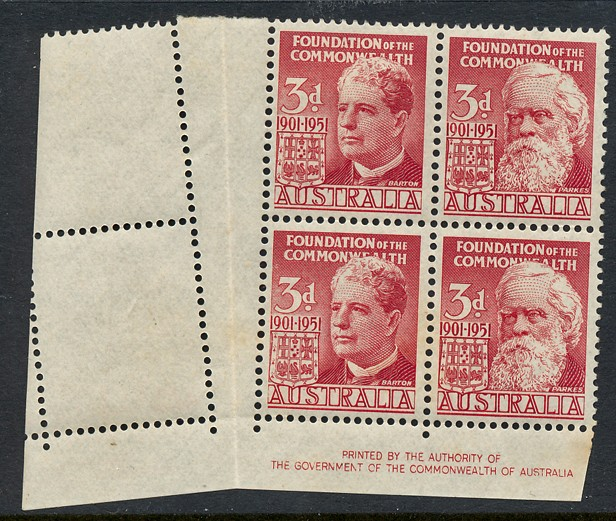
\includegraphics[width=0.7\textheight]{./graphics/australia/SG241var}

{\small \getstampfield{Australia}{SG241var}{description}}


\test{Australia}{SG245-SG245}
\test{Australia}{SG246-SG246}
\test{Australia}{SG247-SG247}
\test{Australia}{SG251-SG252}
%% Aborigines
\test{Australia}{SG253-SG253ba}
%% Scout
\test{Australia}{SG254-SG254}

\test{Australia}{SG255-SG259}

\test{Australia}{SG261-SG263a}
\test{Australia}{SG261-SG263a}
\test{Australia}{SG264-SG266}
\test{Australia}{SG267-SG267}

\test{Australia}{SG270-SG270}
\test{Australia}{SG271-SG271}

\long\def\printLongDescription#1#2{%
  \flushleft%
  \getstampfield{#1}{#2}{longdescription}%
\endflushleft%
}


\printLongDescription{Australia}{SG271}
%Royal Visit
\test{Australia}{SG272-SG274}
\test{Australia}{SG275-SG275}
\test{Australia}{SG276-SG276}
\test{Australia}{SG277-SG277}
\test{Australia}{SG278-SG278}
\test{Australia}{SG279-SG279}

\test{Australia}{SG281-SG281}
\test{Australia}{SG283-SG283}
\test{Australia}{SG284-SG285}
\test{Australia}{SG286-SG286}
\test{Australia}{SG287-SG287}
\test{Australia}{SG288-SG288}
\test{Australia}{SG289-SG289}
\test{Australia}{SG296-SG296}
\test{Australia}{SG297-SG297}
\test{Australia}{SG298-SG299}

%% 300 NUMBERS
\test{Australia}{SG301-SG301}
\test{Australia}{SG302-SG303}

\test{Australia}{SG304-SG304}
\test{Australia}{SG305-SG305}
\test{Australia}{SG306-SG307}
\test{Australia}{SG308-SG308}

\test{Australia}{SG316-SG316}
\test{Australia}{SG322-SG326}
\test{Australia}{SG327-SG327}
\test{Australia}{SG331-SG331}

\test{Australia}{SG332-SG332}
\test{Australia}{SG333-SG333}

%%1960
\test{Australia}{SG334-SG334}


\getsetdetail{Australia}{SG415-SG416}

\getsetdetail{Australia}{SG363-SG369}
\test{Australia}{SG363-SG369}




\test{Australia}{SG370-SG371}

\test{Australia}{SG372-SG372}

\test{Australia}{SG405-SG405}


\test{Australia}{SG415-SG416}
\test{Australia}{SG420-SG425}
\test{Australia}{SG426-SG426}
\test{Australia}{SG427-SG427}
\test{Australia}{SG428-SG429}
\test{Australia}{SG430-SG430}

\test{Australia}{SG431-SG431}

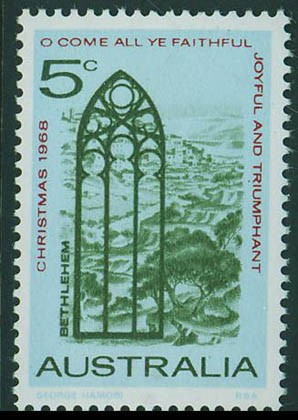
\includegraphics[scale=1.7]{./graphics/australia/SG431a}

\test{Australia}{SG432-SG435}
\test{Australia}{SG436-SG436}
\test{Australia}{SG437-SG437}
\test{Australia}{SG438-SG438}
\test{Australia}{SG439-SG439}
\test{Australia}{SG440-SG443}
\test{Australia}{SG444-SG445}
\test{Australia}{SG446-SG449}

\test{Australia}{SG450-SG452}
\test{Australia}{SG453-SG453}
\test{Australia}{SG454-SG455}
\test{Australia}{SG456-SG457}
\test{Australia}{SG458-SG458}

\test{Australia}{SG459-SG464}

\test{Australia}{SG467-SG468d}
\test{Australia}{SG469-SG472}
\test{Australia}{SG475-SG475}
\test{Australia}{SG476-SG476}
\test{Australia}{SG477-SG478}
\test{Australia}{SG479-SG482}
\test{Australia}{SG483-SG485}
\test{Australia}{SG486-SG486}
\test{Australia}{SG487-SG487}
\test{Australia}{SG488-SG488}
\test{Australia}{SG489-SG489}
\test{Australia}{SG490-SG493}

\getsetdetail{Australia}{SG490-SG493}

\test{Australia}{SG494-SG495}
\test{Australia}{SG496-SG497}

\test{Australia}{SG498-SG504}
\test{Australia}{SG505-SG508}
\test{Australia}{SG509-SG509}
\test{Australia}{SG510-SG513}
\test{Australia}{SG514-SG516}
\test{Australia}{SG523-SG529}

\test{Australia}{SG530-SG531}
\test{Australia}{SG532-SG535}
\test{Australia}{SG536-SG536}
\test{Australia}{SG537-SG540}
\test{Australia}{SG549-SG552a}
\test{Australia}{SG553-SG553}
\test{Australia}{SG554-SG555}
\test{Australia}{SG556-SG559}
\test{Australia}{SG560-SG560}


Total Stamps in database \thestampscounter, \stamps@thecounter

Total sets in database \sets@thecounter

\makeatletter


\newif\if@debug
\@debugtrue

\if@debug TEST \begin{minipage}{1cm} \else \fi
Testing some test
\if@debug TEST \end{minipage} \else \fi

\csname Australia@sets@by@year\endcsname

%% Check if an element is in the list
\def\alist{mary,george,maty, }
\def\lst@IfSubstring#1#2{%
    \def\lst@temp##1#1##2##3\relax{%
        \ifx \@empty##2\expandafter\@secondoftwo
                 \else \expandafter\@firstoftwo \fi}%
    \expandafter\lst@temp#2#1\@empty\relax}

\lst@IfSubstring{mary}{\alist}{yes}{no}


% \begin{macro}{\lst@NormedDef}
% works like |\def| (without any parameters!) but normalizes the replacement
% text by making all characters lower case and stripping off spaces.
%    \begin{macrocode}
\def\NormedDef#1#2{\lowercase{\edef#1{\zap@space#2 \@empty}}}
%    \end{macrocode}
% \end{macro}

\NormedDef\Funny{SG12 - SG13}

\Funny 


%\printindex

a bc b\\n a

\input{stamp-fields}



\newpage

%	Calculate the width of an image by placing it in
%	a box and get its dimensions.
%
\global\newsavebox\imagetestbox
%
%  The image is called with the
%  #1 path
%  It defines three sizes
%  raw@image@widthpt
%  raw@image@width@nopoint
%  all calculations use points and then they are stripped
\def\getimagedimensions#1{%
  \sbox\imagetestbox{\includegraphics{#1}}
  \def\naturaltextwidth{\the\textwidth}
  \def\naturalimagewidth##1{\the\wd##1}
  \def\naturalimageheight##1{\the\ht##1}
  \edef\z{\naturalimagewidth{\imagetestbox}}, 
  \def\y{\naturalimageheight{\imagetestbox}} 
  \def\x{\naturaltextwidth}
  \def\raw@image@width@nopoint{\expandafter\strip@pt\wd\imagetestbox}
  \def\raw@image@height@nopoint{\expandafter\strip@pt\ht\imagetestbox}
  \def\raw@image@width@pt{\the\wd\imagetestbox}
  \def\raw@image@height@pt{\the\ht\imagetestbox}
  \def\aspect@ratio{%
    \FPdiv{\aspectratio@}{\raw@image@width@nopoint}{\raw@image@height@nopoint}
    \aspectratio@
  }
}

\def\GetImageDimensions#1#2{%
  \edef\PathString{./graphics/\csname#1#2@image\endcsname}
  \getimagedimensions\PathString
}
%
% Unfortunately when developing these examples I collected images
% from various places on the web. Not all images have been scanned
% to the same resolution and not all images have been scanned to
% their true size.
%
% Getting the real actual length of an image is difficult, especially
% since the size for most stamps is not know. There are a number of
% approaches that can be used.
%
% If the perforation gauge is known, the size of the stamp can be determined
% by counting the perforations. The perforation scale is based on 
% how many perforations fit in two centimeters.
%  macro get@size@from@perforations
%   
%   #1 13 x 13 perf gauge
%   #3 number of perforations for width + 1
%   For example at 17 perforations for a 13.5x13.5 perforation gauge
%   we get
%	#4 natural image width in pt
%   2.518518518518518518518518
%   the decimals repeat and don't ask me why!
%
\def\get@size@from@perforations#1#2#3#4{%
  \FPdiv\@stamp@width{#3}{#1}%
% 	multiply by 2cm to get the width of the stamp
  \FPmul\@stamp@width{\@stamp@width}{2}
%	round to two decimal places
  \FPround\@stamp@width{\@stamp@width}{2}
%	output the result in centimeters
\@stamp@width cm, 
%  change to points
\FPmul\stamp@width@pt{\@stamp@width}{28.4527559}%
\FPround\stamp@width@pt{\stamp@width@pt}{2}%
\stamp@width@pt pt%
}%
%%	once we know the actual width of the image
%%    we can determine the scalex that the image has been scanned
%%	this is important for calculations later on
%%
%\newlength\tempdimen
%\setlength{\tempdimen}{\@stamp@width cm}\relax}



\def\addnoperforationsx#1#2#3{%
 \expandafter\def\csname#1#2@noperforationsx\endcsname{#3}
}
% getter for obtaining the number of perforations
% if it does not exist assume 18
% this might not be a very good idea
% a better guess is needed
\def\getnoperforationsx#1#2{%
\ifcsname#1#2@noperforationsx\endcsname%
  \@nameuse{#1#2@noperforationsx}%
\else%
17%
\fi
}




\addnoperforationsx{Australia}{SG75}{15}


\GetImageDimensions{Australia}{SG75}

\includegraphics{\PathString}




Number perforations \getnoperforationsx{Australia}{SG75}

natural image width= \z

natural image height=\y

estimated image width= \get@size@from@perforations{13}{13}{\getnoperforationsx{Australia}{SG75}}{\z}

eatimated image height

No point raw width \raw@image@width@nopoint

With point raw width \raw@image@width@pt

No point raw height \raw@image@height@nopoint

With point raw height \raw@image@height@pt

Aspect ratio \aspect@ratio
% get the scale of the stamp image as compared
% to two values
% #1 target value (real size)
% #2 current image size
% round to five decimals places to avoid round off errors 
% 
\def\get@scale#1#2{%
 \FPdiv\stamp@scale{#1}{#2}
 \FPround\stamp@scale{\stamp@scale}{5}
\stamp@scale}
%
%
%

%The scale \get@scale{65.73}{\z}

\z

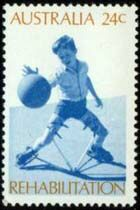
\includegraphics[scale=1.44915]{./graphics/australia/SG516}

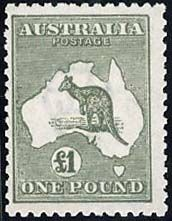
\includegraphics[scale=0.39659]{./graphics/australia/SG75}
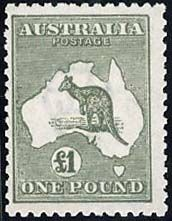
\includegraphics[scale=0.39659]{./graphics/australia/SG75}
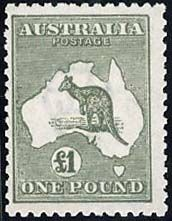
\includegraphics[scale=0.39659]{./graphics/australia/SG75}
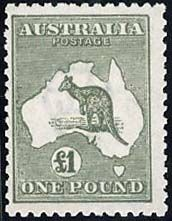
\includegraphics[scale=0.39659]{./graphics/australia/SG75}
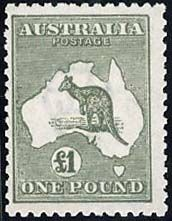
\includegraphics[scale=0.39659]{./graphics/australia/SG75}


\chapter{New Zealand Postal History}

\subsection{Forerunners to the Monthly Packet Service}

Before the normal mails were arranged postmasters availed of ships entering the islands ports to send mail, sometimes via difficult and unpredictable routes.
%% sale details
%  #1 Auctioneer
%  #2 No of sale
%  #3 date of Sale
\long\def\addsale#1#2#3{%
  \expandafter\def\csname#1#2\endcsname{#3}
}

\addsale{Prestige}{165}{Prestige Philately, General Auction 165, 27 May, 2011.}

\long\def\getsale#1#2{%
  %\@nameuse{#1#2}
}




\def\postmark#1{\texttt{#1}}

%% Index commands
\def\NZindex#1{\protect\index{New Zealand!#1}#1}%
\gdef\ship#1{\protect\index{Ships!#1}\textit{#1\xspace}}
\def\people#1{\protect\index{Personalities!#1}#1\xspace}

% Typesetting commands for postal history items.
% this is the general command, it is also possible to customize 
% the styling.
\newcommand\printph[4][0.9]{%

\xdef\imagepath{\getstampfield{#2}{#3}{image}}%
%\marginnote{This is a marginnote}[-60pt]
\hskip210pt\hbox{\footnotesize #2-#3}\vskip1pt
\begin{fullwidth}
\includegraphics[width=#1\textwidth]{./graphics/\imagepath}
%\vskip-130pt\hskip10.2cm\begin{minipage}[t]{3cm}
%This is a lot of margin notes that are fixed to the side
%rather than float around.
%\end{minipage}
\end{fullwidth}
%\vskip55pt
\parindent=1em\small\getstampfield{#2}{#3}{description}
\getsale{Prestige}{165}\par
{\parindent=0pt\flushleft\small\getstampfield{#3}{#3}{ex}\endflushleft}\par


%
}

% Typesetting commands for postal history items.
% this is the general command, it is also possible to customize 
% the styling.
\newcommand\printside[4][0.9]{%

\xdef\imagepath{\getstampfield{#2}{#3}{image}}%
%\marginnote{This is a marginnote}[-60pt]
\hskip210pt\hbox{\footnotesize #2-#3}
\sidenote{\parindent=1em\small\getstampfield{#2}{#3}{description}}
\includegraphics[width=#1\textwidth]{./graphics/\imagepath}
%\vskip-130pt\hskip10.2cm\begin{minipage}[t]{3cm}
%This is a lot of margin notes that are fixed to the side
%rather than float around.
%\end{minipage}
%\vskip55pt
\vspace{0.7cm}
}



\chapter{Late Fees}

\additem{AU}{PH1265}%
{OVERSEAS: (Oct) cover with imprint of Slade Allan \& Co (indent merchants) to New York with KGV 1d green & 1½d red pair tied by superb 'AUCKLAND/LOOSE LETTER' cds (Hosking \#1547; rated C). [From 1922, the late fee was standardised at 1d]}%descrition
{1874}%4
{AU/252933}%5
{}%ex
{}
{}%
{}%


\printph[1.2]{AU}{PH1265}


\chapter{New Zealand Postal History}
\additem{NZ}{PH001}%
{1840 large-part entire headed ``Bay of Islands 21st Feby 1840" to ``George Clendon/Deal/Kent'' with two strikes of the stepped \postmark{EASTBOURNE/SHIP LETTER} h/s \& London b/s of \postmark{18JY18/1840} in red, rated "8" in black for an incoming shipletter, internal splitting and reinforcing. Carried per barque \ship{Westminster} which departed the Bay of Islands 17/3/1840, making a remarkably swift passage of less than 4 months, in an era when voyages of 12 months were commonplace. 

Very few letters from the interim or transitional period between the formal annexation of New Zealand by New South Wales in February 1840 and the opening of the first post office, at \NZindex{Kororarika}, in March 1840 have been recorded. 

The sender was \people{James Clendon}, one of the most prominent early settlers. He settled in the Kororarika (Russell) district in 1832 and in 1838 was appointed United States Consul in New Zealand. 

In 1840 he signed the Treaty of Waitangi as witness to the signatures of several Maori chiefs, and was appointed to New Zealand's first Legislative Council. His property at Okiato was acquired by the new government, but the purchase was only partly-completed and Clendon was compensated with 10,000 acres south of Auckland!! 

This letter was written only two weeks after the original signing on 6th February of the Treaty of Waitangi. In it, Clendon states
\quote
...Our adopted land is now a British Colony. Captain Hobson Lieutenant Governor and Staff arrived on the 29th Jany...It has of course raised the value of land and I hope to turn some of mine to good account. I am probably the largest landholder...Almost every fortnight brings an arrival from Sydney with from 50 to 70 Passengers so that our Bay is getting very thickly populated...I consider my land in the Bay of Islands worth at least \pounds10,000 and a tract between this and the Thames...I would not take less than \pounds20,000...
\endquote
}%
{1874}%4
{NZ/255553}%5
{Ex Barry Scott.}%ex
{}
{}%
{}%


\additem{NZ}{PH002}%
{1847 outer to London with oval \postmark{PAID SHIP LETTER/[crown]/AP*17/1847/SYDNEY} d/s in red on the face, rated "3" in red for an outgoing (from Sydney) shipletter \& "1/-" in black for an inwards (to GB) packet letter, London arrival b/s of 28SP28/1847 in red, docketed as being sent by "W Lawry/Auckland", minor blemishes. Carried per Toulmin packet \textit{Ann Miln} from Sydney 5/5/1847; arrived Plymouth 28/9/1847. 
Illustrated at page 42 of the Handbook Vol VII. 
[The Toulmin Brothers packet service from Sydney operated 42 homeward sailings between 2/1/1846 \& 7/6/1849. New Zealand mails forwarded via Sydney could be carried on a Toulmin sailing. Examples are quite scarce]}%description
{1874}%4
{NZ/255554}%5
{Ex John Bishop Scott.}%ex
{}
{}%
{}%


\additem{NZ}{PH003}%
{1850 (Nov 28) missionary's double-rate entire to London via "Adelaide" but crossed-through and re-endorsed "via Sydney" with light but largely clear strike of the \postmark{/PAID/AT/AUCKLAND NEW ZEALAND} crowned-circle handstamp SG CC1 (Cat \pounds300 on cover) and superb \postmark{AUCKLAND/ A /=NEW-ZEALAND=} b/s, rated "8" in red and "1/-" in black for an inwards packetletter, London arrival b/s of 3MY3/1850 in red, docketed as from "J~Hobbs/Auckland". 

Carried from Sydney by private ship, the Toulmin Brothers service having ended in June 1849, and the ARMSN sailings commencing only in September 1852.
\index{Toulmin Brother Service}
}%description
{1850}%4
{NZ/255555}%5
{}%ex
{}
{}%
{}%

\additem{NZ}{PH004}%
{1852 (Aug 18) entire headed "at Mr Jackson's/River Heathcote/Canterbury/New Zealand" to London "via Wellington \& Sydney" with light but largely obvious strike of the '[crown]/PAID/AT/PORT VICTORIA/NEW ZEALAND' crowned- circle handstamp SG CC6 (Cat £1200 on cover) in red \& similarly light strike of the \postmark{PORT- VICTORIA/ NEW-ZEALAND} b/s, rated "2" in red \& "1/-" in black for an inwards packetletter, faint London arrival b/s in red. Carried per Australian Royal Mail Steam Navigation Co packet \ship{Australian} out of Sydney 20/9/1852; arrived Plymouth 11/1/1853. This was the first of only three contract - and three non-contract - ARMSN sailings over a period of two years. Covers from New Zealand carried per ARMSN - the first steam packet service from Australia - are very scarce. The outwards shipletter rate was halved from 4d to 2d in April 1851. The letter, signed "Wendell [?] 

Draper" states "...the Australian Diggings have drawn from here a large part of the population...Many people who have made small fortunes on the gold field have come here to invest so that eventually the diggings may repay us for all the evil they have hitherto done us in various ways..."}%descrition
{1850}%4
{NZ/255556}%5
{}%ex
{}
{}%
{}%

\additem{NZ}{PH005}%
{1856 (Jan 4) cover to Leicester "via Sydney/Wm Denny" with a largely fine strike of the '[crown]/ PAID/AT/AUCKLAND NEW ZEALAND' crowned-circle handstamp SG CC1 (Cat £300 on cover) and very fine 'AUCKLAND/ A /=NEW-ZEALAND=' b/s (day slug twice), very fine '2' h/s in red applied at Auckland \& '6' h/s applied at Liverpool, superb 'AUSTRALIAN/LIVERPOOL/AP26/1850/=PACKET=' transit \& 'LEICESTER' arrival b/s in blue, minor defects. [Between August 1854 \& March 1857, the Auckland Provincial Government contracted with the owners of the steamship \ship{William Denny} for a monthly service between Auckland and Sydney to connect with the English mails. Between June 1855 and mid-1856 the Black Ball Line and White Star Line alternated twice-monthly clipper sailings between Liverpool \& Sydney. However, the return sailings were uncontracted. Despite being treated as private voyages, the Liverpool packet cds was often applied on arrival]}%descrition
{1850}%4
{NZ/255557}%5
{}%ex
{}
{}%
{}%

\additem{NZ}{PH006}%
{1856 (Feb 14) outer to London "pr Southern Cross via Talcahuano/and Panama" with London Printing 2d dull blue on Blued Paper SG 2 (margins just clear to large) tied by indistinct cancel of Wellington (b/s), London arrival b/s of 1856/17MY17 in red, rated "2/-" for a double-weight inwards packetletter. 

Ex Michael Burberry (1986), Gerald Ellott \& John Woolfe (Lot 283; acquired for £4465). A remarkable and highly important cover. 

[This was the original of the letter, the duplicate of which is the next lot!]ÞÞNumber 39 in Robin Gwynn's 2005 census of 67 covers and dated pieces from the first year of use of New Zealand stamps. This cover was carried on the only Chalons Period mail-carrying voyage via South America. 

It is illustrated in the Handbook Vol VII at page 62. Only one other such cover is recorded. ÞÞIt is possible that this cover, instead of travelling north to Panama along the west coast of South America, was actually carried overland to Buenos Aires. Howat at page 131 of "South American Packets 1808-1880" states that the \ship{Avon} departed Buenos Aires 3/4/1856 \& Rio de Janeiro 15/4/1856, arriving at Southampton 16/5/1856, the day before the London arrival cds. While this is not conclusive evidence, it is highly relevant that Kenton \& Parsons "Early Routings of the Royal Mail Steam Packet Company 1842-1879" list no arriving steamer from Panama that fits comfortably with the 17/5/1856 receival on this cover. As they say in the classics: "The thick plottens!"ÞÞHistorical note: on 27/2/2010, the Chilean port of Talcahauno was largely destroyed by a massive earthquake and tsunami.}%descrition
{1850}%4
{NZ/255558}%5
{}%ex
{}
{}%
{}%

\additem{NZ}{PH007}%
{1856 (Mar 7) envelope to London "p Seringapatam/direct" (also endorsed \textit{D orig pr Southern Cross via Panama} with London Printing 2d dull blue on Blued Paper SG 2 (insignificant corner crease, otherwise a superb stamp with good to large margins, lifted \& hinged back into place) tied by indistinct cancel of 'WELLINGTON' (b/s), rated "6" in black payable on arrival, London transit \& very fine strike of scarce 'BRISTOL/JU17/1856/ K /=IN=' (Robertson Revisited \#S10; ERD). 

A famous cover: Number 46 in Robin Gwynn's 2005 census. It is illustrated by Odenweller at page 27. Holcombe Certificate (1988). This and the previous lot - posted three weeks earlier - represent a remarkable re-uniting of original \& duplicate mailings.

This was a very common commercial practice in an age when shipwrecks were all too frequent. However, it is most unusual for both such items to be found together. Indeed, with the previous item having been discovered only in the 1980s, our vendor is confident that he is the first person to own both of them. While it may seem odd that the original should have been sent via an exotic and unproven route, it must be remembered that during the Crimean War mails from Australia, and even moreso from New Zealand, were seriously affected by a lack of available ships. The sender doubtless chose to avail himself of the "first ship" opportunity, regardless of the fact that it was sailng eastwards, across the Pacific.}%descrition
{1850}%4
{NZ/255559}%5
{Ex Maurice Burrus (Lot 33), Bob Odenweller (private transaction), "Antipodes" (Lot 3151) \& Hackmey II (Lot 2050)}%ex
{}
{}%
{}%


\additem{NZ}{PH008}%
{1856 (April 30) cover to Hampshire with London Printing 2d dull blue on Blued Paper SG 2 (margins just touched - at upper-right - to large) tied by indistinct cancel of 'AUCKLAND' (b/s), rated "8" in black, London transit b/s \& fine 'KINGSCLERE/AU14/1856' arrival cds in blue on the face. Number 54 (?) in Robin Gwynn's 2005 census. Ex WT Wilson (?) \& John Woolfe (Lot 196: acquired for £420). [In the Woolfe catalogue, it was stated that the cover was carried for part of the journey per the \ship{Royal Charter}, an auxiliary steam-screw vessel of the \index{Eagle Line}Eagle Line]}%descrition
{1856}%4
{NZ/255560}%5
{}%ex
{}
{}%
{}%

\additem{NZ}{PH009}%
{1856 (June 8) mourning cover to Westmoreland - unusually with no shipping endorsement - with London Printing 2d dull blue on Blued Paper SG 2 (three good margins but a little cut-into at left) tied by light '17' cancel of Christchurch (no b/s "tie"), fine 'PORT VICTORIA' b/s, rated "8" in black, London \& fair 'PENRITH' (in blue) transit backstamps. Attractive. Port Victoria (originally named Port Cooper) PO 8/8/1849; renamed Lyttelton 2/3/1858. Number 58 in Robin Gwynn's 2005 census. Ex Goodfellow \& "Yeroc" (Royce Bowen). 

[Lyttelton remains the port for Christchurch but on 22/2/2011 suffered severe earthquake damage]}%descrition
{1856}%4
{NZ/255561}%5
{"Yeroc" (Royce Bowen}%ex
{}
{}%
{}%

\additem{NZ}{PH010}%
{1856 (Dec 4) entire headed "Christchurch/Canterbury" \& signed "Fanny FitzGerald", to London with Richardson Printing on Blue Paper 2d blue SG 5 (a beautiful stamp with almost full margins, just touched at lower-right) just tied by crisp '16' cancel of 'PORT VICTORIA' (fine b/s), rated "6" in black, London arrival b/s of 9MY9/1857 in red, minor internal repairs. 

Ex Hugh Gordon Kaye (Lot 194). An important cover, being carried on the first homeward voyage by the monthly packet mail, per the E\&ARM Co steamer \index{Oneida} that departed Sydney 23/1/1857 carrying a small quantity of New Zealand mail dated the previous month. The five months transit time was due to the \textit{Oneida} breaking down 400 miles off the Western Australian coast and returning to Sydney!! The \ship{Simla} had already sailed so the mail was put aboard the \ship{European} which departed Sydney 11/3/1857!; mails arrived 8/5/1857.

The sender was \people{Frances Erskine FitzGerald} who arrived at Port Victoria on 16/12/1850 on the \ship{Charlotte Jane}. An educated woman, she spoke several languages and was considered a competent painter \& musician. She was a member of the Wellington Ladies' Christian Association and various charities. The wife of James Edward FitzGerald, the founding editor of the "Lyttelton Times" \& first Superintendent of the Province of Canterbury, she bore 13 children. However, from her handwriting, one would swear she was a man! She states "We only received the Mariner's Mail yesterday. She was 140 days out \& was obliged to touch at Hobart Town for water...How very tiresome for the Museum to have come into such a state...[her husband had been assistant secretary at the British Museum]..."}%descrition
{1850}%4
{NZ/255562}%5
{}%ex
{}
{}%
{}%

\additem{NZ}{PH011}%
{1857 (Jan 22) mourning outer to Scotland with Richardson Printing on Blue Paper 2d blue SG 5 (margins just touching - at upper-left \& lower-right - to large) tied by very fine '1' cancel of 'AUCKLAND' (b/s), rated "6" in black, London transit \& superb 'ABERDEEN/AP10/1857' arrival b/s in green. Carried per "Simla", departed Sydney 11/2/1857; mail arrived Southampton 9/4/1857. }%descrition
{1857}%4
{NZ/255563}%5
{}%ex
{}
{}%
{}%

\additem{NZ}{PH012}%
{1858 (Jan 25) cover to Ireland with Blue Paper 2d blue SG 5 vertical strip of 3 (margins at places), unusual manuscript cancellation (unrecorded by Wooders) with large-part '[BL]UFF HARBOR/JA25/1858/NEW-ZEALAND' b/s, Dublin arrival b/s of AP7/1858. A rare cover. Ex "Emerald" (David Feldman): Lot 40911 (acquired for SFr1298 (2003). RPSofL Certificate (1978) states "despite the lack of tying is genuine". Bluff Harbor (American spelling) is 27km S of Invercargill, close to the southern-most point of the South Island. The PO opened as Bluff 1/3/1856; renamed Bluff Harbor 28/1/1857; closed 20/11/1858. Carried per \ship{Simla}, departed Sydney 11/2/1858; mail arrived Southampton 6/4/1858. 

This is a very early manuscript cancelled cover: John Woolfe's earliest such cover was from 1862.}%descrition
{1857}%4
{NZ/255564}%5
{}%ex
{}
{}%
{}%

\additem{NZ}{PH013}%
{1858 (Mar 19) cover to London endorsed "Ahuriri 16 3 58" at lower-left with White Paper 2d blue SG 10 horizontal strip of 3 from the upper-right of the sheet (margins just clear to enormous), light '11' cancels \& largely very fine 'AHURIRI/NEW ZEALAND' b/s, the strip just tied by London arrival cds of JY19/58 in red, addressee's docketing on the face clear of the stamps. Ex Benjamin Goodfellow (22/5/1950: Lot 44). PO 27/2/1852; renamed Napier 2/3/1858 but the Ahuriri cds continued in use for some time. Carried per "European", departed Sydney 11/5/1858; mail arrived Southampton 18/7/1858. }%descrition
{1857}%4
{NZ/255565}%5
{}%ex
{}
{}%
{}%


\additem{NZ}{PH014}%
{1858 (April 15) part-entire to London with White Paper 2d deep ultramarine SG 8a horizontal strip of 3 (good to large margins, the first unit damaged at the base, Cat £2700++ x2+ on cover) just tied by '18' cancels of Dunedin, London arrival cds of AU14/58 in red on the face, some staining from the writing ink. BPA Certificate (1999). Carried per "Australasian", departed Sydney 11/6/1858; mail arrived Southampton 14/8/1858. [From 27/3/1857, it was compulsory to prepay the postage. The new rate was 6d per ½oz, and there was no longer an inwards fee payable by the recipient]

The BPA Certificate states the stamps are SG 10. However, we agree with our vendor's assessment of the shade as being "deep ultramarine" SG 8a, which also accords with the statement in the Kaye sale (1991). We would allow an extension to obtain a new certificate. }%descrition
{1857}%4
{NZ/255566}%5
{Ex Williams \& Hugh Gordon Kaye (Lot 278).}%ex
{}
{}%
{}%

\additem{NZ}{PH015}%
{1858 (May 19) double-rate cover to London with late usage of London Printing 1/- yellow-green on blued paper SG 3 (margins just touching to large except at right where cut-into, Cat \pounds{5500} x2+ on cover), light '18' cancel \& largely fine 'OTAGO/NEW ZEALAND' b/s used at Dunedin, London arrival cds of AU16/58 in red. Ex Hugh Gordon Kaye (Lot 170). Robert Odenweller Certificate (2006). PO 17/6/1848. Carried per \ship{Australasian}, departed Sydney 11/6/1858; mail arrived Southampton 14/8/1858.}%
{1857}%4
{NZ/255567}%5
{}%ex
{}
{}%
{}%
\additem{NZ}{PH016}%
{1858 (Aug 24) cover to Wiltshire with White Paper 2d blue SG 10 single \& pair (all with full margins, a couple of tiny defects), neat '1' cancels \& largely very fine Auckland cds on the face, 'CALNE/NO13/58' arrival b/s. Carried per \ship{European}, departed Sydney 11/9/1858, the third sailing under the Royal Mail; mail arrived Southampton 11/11/1858}%descrition
{1857}%4
{NZ/255568}%5
{}%ex
{}
{}%
{}%

\additem{NZ}{PH017}%
{1859 (Jan 29) cover to Wiltshire with White Paper 2d pale blue SG 9 horizontal strip of 3 (margins just shaved - at base - to large), Auckland b/s \& 'CALNE/AP11/59' arrival b/s. Ex Marcel Stanley (Lot 510). Carried per \ship{Salsette}, the first pre-contract P\&O voyage, departed Sydney 12/2/1859 via Melbourne, Adelaide, Albany, Mauritius, Aden \& Suez, mail arrived Southampton 9/4/1859.}%descrition
{1857}%4
{NZ/255569}%5
{}%ex
{}
{}%
{}%

\additem{NZ}{PH018}%
{1859 (Aug 9) cover to Scotland with White Paper 2d pale blue SG 9 horizontal strip of 3 (shaved at top \& a little cut-into at right), poor '18' cancels, very fine 'OTAGO' b/s used at Dunedin \& ' U M/EDINBURGH/NO11/59' arrival b/s. Carried per "Bombay", departed Sydney 14/9/1859, mail arrived Southampton 10/11/1859.}%descrition
{1857}%4
{NZ/255570}%5
{}%ex
{}
{}%
{}%

\additem{NZ}{PH019}%
{1859 (Oct 1) cover to Scotland with White Paper 6d pale brown SG 14 (margins good to large with a fragment of the adjoining unit below, small corner fault at upper-right, Cat £300 x2+ on cover)) tied by neat '15' cancel of 'NELSON' (b/s), poor Dundee arrival b/s of DE15/1859, a few ironed-out creases that just impact the stamp at lower-left. Ex Hugh Gordon Kaye (Lot 288). Carried per "Emeu", departed Sydney 14/10/1859, mail arrived Southampton 14/12/1859.}%descrition
{1857}%4
{NZ/255571}%5
{}%ex
{}
{}%
{}%

\additem{NZ}{PH020}%
{1862 (Sep 12) distressed cover with light Wellington b/s, the stamp washed-off (at upper-left), very fine strike of the boxed \postmark{Saved from the wreck of/the Colombo} h/s on the face, London arrival cds of DE31/58 in red on the face, despite the faults an attractive wreck cover. Carried per \ship{Bombay}, departed Sydney 22/10/1862, for Galle, then per \ship{Colombo} which was wrecked off Minicoy Island in the Laccadives on 19/11/1862. This item was put aboard \ship{Nemesis} or \textit{Ottawa} direct to Suez, then per \ship{Massilia} from Alexandria 16/12/1862, arrived Southampton 30/12/1862. From 14/3/1860, the P\&O route was varied to Sydney-Melbourne-Albany-Galle. [This was the first incident involving Australasian mail to which a wreck cachet was applied. See also Lots 34 \& 35]}%descrition
{1857}%4
{NZ/255572}%5
{Ex Gerald Ellott.}%ex
{}
{}%
{}%

\additem{NZ}{PH021}%
{1865 (Apr 29) cover with printed address to London with very fine Imperf 6d red-brown (margins good to large lightly cancelled with fine Auckland duplex, London arrival b/s of JY22/65, minor blemishes. Carried per \ship{Madras}, departed Sydney 22/5/1865; mail arrived Southampton 22/7/1865. ["Antipodes" very similar cover with a larger imperf 6d (Lot 3402) sold for SFr1650 in 1988!]}%descrition
{1865}%4
{NZ/255714}%5
{Ex Gerald Ellott.}%ex
{}
{}%
{}%

\additem{NZ}{PH022}%
{1865 (July 31) cover to Ireland endorsed "Registered 402" in red with Perf 12½ 6d brown \& Imperf 1/- yellow-green (margins close to large except where just touched at the top) tied by light numeral cancels of 'WANGANUI' (b/s), 21mm Wellington transit b/s of AU5/1865 \& superb 'GALWAY/OC23/65' arrival b/s, ironed-out horizontal crease, repaired faults on the reverse \& to the left of the stamps. Ex "Emerald" (David Feldman): Lot 40917 (acquired for SFr2360 (2003). Carried per \ship{Jedda}, departed Sydney 22/8/1865, mail arrived Southampton 22/10/1865. [From 24/6/1857, the registration fee was 1/- in addition to the postage payable]}%descrition
{1865}%4
{NZ/255573}%5
{Ex Emerald.}%ex
{}
{}%
{}%

\additem{NZ}{PH023}%
{Description: 1866 (Aug 17) mourning cover to Hampshire with Perf 13 (?) 6d brown (corner fault) tied by indistinct cancel of Christchurch (b/s) \& 'SOUTHAMPTON/OC20/1866/PACKET LETTER' cds, 'BASINGSTOKE' arrival cds on the face. Ex Gerald Ellott. Carried per \ship{Bombay}, departed Melbourne 28/8/1866, mail arrived Southampton 20/10/1866. [Between June 1866 \& December 1868, most mail from NZ went by the trans-Pacific route via Panama. In this period, covers via Suez are relatively scarce. According to "Robertson Revisited", the Packet Letter cds indicates that the cover was received as a loose letter]}%descrition
{1865}%4
{NZ/255575}%5
{}%ex
{}
{}%
{}%

\additem{NZ}{PH024}%
{1867 (Oct 19) mourning cover to Scotland with Perf 12½ Plate II 2d deep blue \& 4d yellow just tied by '18' cancels (superb strike on the 4d) of 'PORT CHALMERS/OTAGO NZ' (superb b/s), light strike of British ' C /RPO/FD' railway TPO h/s (Harold Wilson \#644) in red \& 'EELON/DE20/67' arrival cds on the face. Most attractive. Carried per \ship{Avoca}, departed Melbourne 28/10/1867, mail arrived Southampton 19/12/1867. [Official Post Office figures for 1867 show that in most months less than 30\% of mail from NZ went via Suez. The TPO h/s was issued to the Inland Branch of the London GPO, for use on letters addressed to destinations north of Perth: see Harold Wilson at page 169]}%descrition
{1865}%4
{NZ/255576}%5
{}%ex
{}
{}%
{}%

\additem{NZ}{PH025}%
{1868 (Nov 19) cover to Scotland endorsed "Registered/1054" in red with Perf 12½ 6d red-brown \& 1/- yellow-green tied by fine '20' cancels of 'GREYMOUTH' (b/s; no year slug), Christchurch (DE3/68) \& Glasgow (JA29/69) transit b/s \& light 'GOVAN' arrival b/s, repaired opening tear at upper-left \& part of the flap missing. Carried per \ship{Geelong}, departed Melbourne 9/12/1868, mail arrived Southampton 29/1/1869.}%descrition
{1865}%4
{NZ/255574}%5
{}%ex
{}
{}%
{}%

\additem{NZ}{PH026}%
{1869 (Feb 20) cover to Yorkshire with Perf 12½ 3d deep mauve SG 118 tied by 'C'-in-Bars cancel and Christchurch cds alongside, endorsed "Detained for postage" in red, a second example of the 3d affixed \& similarly cancelled with a second Christchurch cds of MR13/69!, largely very fine strike of the scarce British 'SW/YORK/MY23/69' railway TPO b/s (Harold Wilson \#629a) used on the seasonal Scarborough \& Whitby Sorting Carriage: see Wilson at page 163. Another very attractive cover. Ex "Antipodes" (Lot 3583). Holcombe Opinion (1988) states the stamps are SG 117 but see the next lot. Carried per "Avoca", departed Melbourne 30/3/1869, mail arrived Southampton 22/5/1869. [The Panama New Zealand \& Australian Royal Mail Co failed in late-1868. Until the via San Francisco route was established in March 1870, via Suez was again the primary route for mails from New Zealand]}%descrition
{1865}%4
{NZ/255577}%5
{}%ex
{}
{}%
{}%

\additem{NZ}{PH027}%
{1869 (Apr 19) cover to Ireland with Perf 12½ 3d lilac SG 117 x2 tied by first type 'WELLINGTON - 070 ' duplex, the flap removed \& black marks on the reverse that don't detract from the fine appearance. Presumably carried per "Malta", departed Sydney 22/4/1869, mail arrived Southampton 18/6/1869. [No photo]}%descrition
{1865}%4
{NZ/25558}%5
{}%ex
{}
{}%
{}%

\additem{NZ}{PH028}%
{1872 (Sep 4) triple-rate cover to London endorsed "via Suez" with Perf 12½ 6d pale blue SG 136 single \& pair tied by ' D /NZ/DUNEDIN - 0 ' duplex, London arrival cds of 4/11/1872 in red on the face. Ex "Antipodes" (Lot 3688). Carried per \ship{Tanjore}, departed Melbourne 11/9/1872, mail arrived Southampton 4/11/1872. Holcombe Opinion (1988) erroneously states the stamps are a strip of 3. [The via San Francisco route commenced out of Sydney 26/3/1870. Apart from a short period in 1873 when the trans-Pacific route was in a state of chaos, the via Suez route was again relegated to a secondary route for mails from New Zealand, and then principally for mail originating from the South Island]}%descrition
{1865}%4
{NZ/255579}%5
{}%ex
{}
{}%
{}%

\additem{NZ}{PH029}%
{1873 (Feb 11) cover to Scotland endorsed "via Suez" with Perf 12½ 2d vermilion x3, poor cancels of 'BALCLUTHA/OTAGO NZ' (largely fine b/s), Dunedin transit \& 'DUNSE/AP23/73' arrival b/s, flap fault \& small repaired opening faults at the top well clear of the stamps. Carried per \ship{Mooltan}, departed Melbourne 28/2/1873, mail arrived Southampton 21/4/1873. Balclutha PO 14/11/1865.}%descrition
{1865}%4
{NZ/255580}%5
{}%ex
{}
{}%
{}%

\additem{NZ}{PH030}%
{1873 (May 27) to Worcestershire endorsed "Via Suez" with extremely rare franking of Perf 12½ 2d orange SG 133 \& 6d pale blue SG 136, '5' cancels of 'TIMARU' (fine b/s), Christchurch transit b/s (affected by flap fault) \& superb 'MALVERN/AU13/73' arrival b/s, minor wrinkling. Carried per \ship{Bangalore}, departed 18/6/1873, mail arrived Southampton 12/8/1873. [Tabeart at page 246 notes that the Galle steamer, in this case "Peshawar", passed through the Suez Canal \& continued to Southampton. The mails, however, had been off-loaded at Suez. The all-sea portion was then re-loaded onto the same ship at Alexandria!]

This is an intriguing cover. Gerald Ellott (2009) at pp217-8 cites research by Mark Benvie as proving the existence of a previously unrecorded 8d rate that came about as the result of an erroneous notice in "The Timaru Herald" of 22/5/1873. The error was corrected in the same newspaper only two days later, making this perhaps the shortest-lived "rate" in all of New Zealand postal history! Copies of the newspaper notices of 2/5/1873 \& 27/5/1873 are included. This is believed to be the only recorded cover at this phantom "rate". [A former owner's notations on the reverse state "From Otaio Station/Auckland Militia/Going to Ch Ch/Perhaps up the Mackenzie/Rosario Tipkins"]}%descrition
{1865}%4
{NZ/255582}%5
{}%ex
{}
{}%
{}%

\additem{NZ}{PH030a}%
{Lot No. 2671
1873 (June): Cover from Westland to Locarno, Switzerland via Suez, franked by two horizontal pairs of 1871 2 d. orange, perf. 12 1/2, tied by bold strikes of rare "W" handstamp of Westland. The stamps have been lifted for checking and carefully replaced, with slight tear in perfs. of the left hand pair. London transit cds (Sept 9) in red on front of cover alongside "PD" in same ink, with manuscript "2 d." at upper left being the credit to Britain and further mss. '20' (centimes) being the credit to France. Reverse with Hokitika cds (June 30), Christchurch transit (July 2) and Locarno arrival (Nov 11) datestamp. Some ageing to envelope and small piece removed from reverse, however a rare 'Goldrush' cover to Switzerland with no similar item recorded. Note: In 1873 the usual via San Francisco route was interrupted and the rate to Switzerland via Suez was officially 9 pence, as introduced in November 1871. The British share on this cover is noted clearly as 2 pence, so it has to be assumed that the reduction in rate to 8 pence (officially pronounced on Jan 1, 1874) was already in force. Provenance: Collection H. Dumas. Collection Silvain Wyler. 
Corinphila Auction Catalogue December 2010 }%descrition
{1865}%4
{NZ/2671}%5
{}%ex
{}
{}%
{}%



\additem{NZ}{PH031}%
{ 1873 (Oct 23) flapless double-rate cover to London with Perf 12½ 1/- yellow-green (cut from the sheet at top to preserve the design) tied by light 'NZ/HOKITIKA - C/21' duplex, part-Christchurch transit b/s \& London arrival cds of 30DE73 in red on the face. Carried per \ship{Baroda}, departed Melbourne 7/11/1873, mail arrived Southampton 30/12/1873.}%descrition
{1865}%4
{NZ/255583}%5
{}%ex
{}
{}%
{}%

\additem{NZ}{PH032}%
{1874 (Jan 9) double-rate cover to Hertfordshire with outstanding two-issue franking of Perf 12½ 6d blue \& First Sidefaces Perf 12½ 6d blue SG 156 tied by bold ' E /NZ/CHRISTCHURCH - C ' duplex, fine 'WALTHAM CROSS/MR24/74' b/s, minor vertical bend that is barely noticeable, neat docketting on the face. Carried per \ship{Pera} departed Melbourne 29/1/1874, mail arrived 2Southampton 3/3/1874. 

This is an item of great significance, being the earliest recorded cover bearing any First Sideface stamp: the issue date was 2nd January.}%descrition
{1865}%4
{NZ/255581}%5
{}%ex
{}
{}%
{}%

\additem{NZ}{PH033}%
{1861 (July 6) large-part outer (one back panel removed) to Staffordshire "per Prince Alfred" with very fine White Paper Imperf 6d pale brown SG 14 pair (margins just touched - at the base of the second unit - to large) tied by '16' cancel of 'LYTTELTON' (very fine b/s), light 'HIGHAM FERRERS/SP16/61' arrival b/s, small fault at lower-left. Ex Marcel Stanley (Lot 520). Carried per \ship{Northam}, departed Sydney 27/7/1861: mail arrived Marseilles 13/9/1861 \& Southampton mail arrived 19/9/1861. [Prior to September 1863, the rate was the standard 6d per ½oz plus 3d per ¼oz for the cross-France portion, so this item weighed less than ½oz. From 14/3/1860, the P\&O route was varied to Sydney-Melbourne-Albany-Galle]}%descrition
{1865}%4
{NZ/255584}%5
{}%ex
{}
{}%
{}%

\additem{NZ}{PH034}%
{1862 (Aug 26) distressed Christchurch Club cover to Cornwall endorsed "Via/Marseilles" with the stamps washed-off but with an offset impression of a 1d orange on the reverse!, superb 'LYTTLETON' cds unusually on the face, superb strike of the boxed 'Saved from the wreck of/the Colombo.' handstamp on the flap but unusually with no London arrival datestamp. An attractive example. Ex Gerald Ellott. [This was the first incident involving Australasian mail to which a wreck cachet was applied. Carried per \ship{Bombay}, departed Sydney 22/10/1862, for Galle, then per \ship{Colombo} which was wrecked off Minicoy Island in the Laccadives on 19/11/1862]}%descrition
{1865}%4
{NZ/255593}%5
{}%ex
{}
{}%
{}%

\additem{NZ}{PH035}%
{1862 (Sep 6) distressed cover to Surrey with two stamps washed-off but with an unusually large Rouletted 1d vermilion SG 47 (?) still in place, Auckland b/s, London arrival cds of JA16/63 in red on the face \& superb large-part strike of the boxed 'Saved from the wreck of/the Colombo.' handstamp on the flap. A highly desirable partial-franking! Ex Gerald Ellott. [Probably carried to London per \ship{Valetta}, as the London cds most closely conforms to that arrival by reference to Brian Peace's table at page 52. See also Lot 20]}%descrition
{1865}%4
{NZ/255594}%5
{}%ex
{}
{}%
{}%

\additem{NZ}{PH036}%
{1862 (Nov 14) cover to London with attractive 3-colour franking of Large Star Imperf 1d vermilion (3 margins), 2d deep blue (3 large margins but cut-into at the base) \& 6d black-brown x2 (both with full margins, the stamp at upper-right an unusually large example but with a minor corner fault at lower-right) tied by fine '16' cancels of 'LYTTELTON' ('PAID' excised), arrival b/s of JA15/63 in red, minor flap faults. Ex John Woolfe (Lot 255: acquired for £977). Carried per \ship{Madras}, departed Sydney 22/11/1862: mail arrived Marseilles 13/1/1863 \& Southampton mail arrived 17/1/1863. 

[In the Woolfe catalogue, it was stated that postage was 3d overpaid for a 1oz letter. That is incorrect: it was 3d overpaid for a ½oz letter for which the rate was 6d up to ½oz + 3d per ¼oz x2 = 1/-]}%descrition
{1865}%4
{NZ/255586}%5
{}%ex
{}
{}%
{}%

\additem{NZ}{PH037}%
{1863 (July 11) cover to Scotland with attractive franking of Perf 13 at Dunedin 1d orange-vermilion \& 2d pale blue single \& strip of 3, '016' cancels \& fine double-circle 'GOLD FIELD/A/OTAGO NZ' backstamp used at Waitahuna, 'NZ/DUNEDIN/OTAGO/JY14/63' transit \& '1 Y/EDINBURGH/SP14/63' arrival b/s, some very minor soiling. Waitahuna PO 15/10/1861; renamed Waitahuna Gully 1/12/1876. Carried per \ship{Bombay}, departed Sydney 22/7/1863: mail arrived Marseilles 12/9/1863 \& Southampton mail arrived 17/9/1863. [This item weighed less than ¼oz so obviously didn't contain any gold!] 

The Handbook Vol VII at page 166 illustrates three 'GOLD FIELD/OTAGO NZ' cds with codes 'A' 'B' or 'C'. There was also a 'D'. They were used at Waitahuna, Weatherstone, Waipori \& Manuherikia respectively.}%descrition
{1865}%4
{NZ/255585}%5
{}%ex
{}
{}%
{}%

\additem{NZ}{PH038}%
{1863 (Aug 13) cover to Scotland with attractive 3-colour franking of Perf 13 1d vermilion, 2d pale blue \& 6d black-brown tied by '016' cancels, largely very fine double-circle 'GOLD FIELD/A/OTAGO NZ' backstamp used at Waitahuna, 'NZ/DUNEDIN/OTAGO/AU15/63' transit b/s unusually in red, superb 'DEFICIENT POSTAGE ("3")/FINE ("6")' h/s in red \& mss "9d", British 'MORE/TO/PAY' h/s \& '4 Y/EDINBURGH/OC15/63' arrival b/s, minor soiling. Carried per \ship{Madras}, departed Sydney 22/8/1863: mail arrived Marseilles 13/10/1863 \& Southampton mail arrived 20/10/1863. 

[This item weighed between ¼oz \& ½oz so was 3d underpaid, the fine being an additional 6d or double the deficiency]}%descrition
{1865}%4
{NZ/255587}%5
{}%ex
{}
{}%
{}%

\additem{NZ}{PH039}%
{1864 (Feb 13) double-rate cover to "Flintshire/North Wales" with Imperf 2d blue Plate I Worn Plate (margins good to large with a fragment of the adjoining unit below) \& 6d red-brown x3 (all with faults) tied by 'CHRISTCHURCH/NEW ZEALAND - CHCH' duplex, 'HOLYWELL/AP13/64' arrival cds on the face, opened-out. Ex Gerald Ellott. Carried per \ship{Madras}, departed Melbourne 25/2/1864: the mail arrived Marseilles 11/4/1864 and the Southampton mail arrived 16/4/1864. 

[From 12/9/1863, the rate via Marseilles was varied to 6d + 4d per half- ounce, in effect an all-up rate of 10d per ½oz: see Ellott at page 95]}%descrition
{1865}%4
{NZ/255588}%5
{}%ex
{}
{}%
{}%

\additem{NZ}{PH040}%
{865 (Feb 25) cover to Middlesex with Perf 13 2d Plate I Worn Plate vertical pair (toned perfs) \& 6d red-brown tied by 'TAURANGA/NEW ZEALAND' cds (another strike on the reverse), Auckland transit cds unusually on the face, on arrival readdressed to London with Plate '60' 1d (creased before use) affixed \& tied by 'UXBRIDGE/MY16/55 - 830' duplex, London arrival b/s, minor repaired flap fault. Second Maori War cover. Carried per \ship{Northam}, departed Sydney 22/3/1865: mail arrived Marseilles 12/5/1865 \& Southampton mail arrived 19/5/1865. 

The sender was Private Aubrey Vernon of the 3rd Waikato Regiment, and a clerk with the Imperial Commissariat Corps. Tauranga was one of the last areas of fighting during the Waikato War \& remained as the local military headquarters for some time because of continuing skirmishes in the Ureweras. Vernon was a witness in a case against another militiaman accused of theft]}%descrition
{1865}%4
{NZ/255589}%5
{}%ex
{}
{}%
{}%

\additem{NZ}{PH041}%
{1868 (Mar 24) cover with Otago Daily Times imprint on the flap, to London with Perf 12½ 1d vermilion x2, 2d blue Plate I Worn Plate (creased before being affixed) \& 6d red-brown tied by ' K /NZ/DUNEDIN - O ' duplex, 'PAID/MY 18 68/NW/LONDON' arrival cds in red on the face, a few faults \& repairs. Ex Gerald Ellott. Carried per "Geelong", departed Melbourne 31/3/1868: mail arrived Marseilles 16/5/1868 (Tabeart at page 233) \& Southampton mail arrived 23/5/1868. 

The sender was Julius Vogel, who was replaced as editor of the \textit{Otago Daily Times} only a month after this letter was written. A supporter of provincial development, he urged the South Island to secede from the North Island, but later shifted direction to champion provincial rights. As a member of parliament he rose to be Colonial Treasurer, \& Postmaster-General, in which role he was an advocate of trans-Pacific mail routes. From April 1873 to July 1875, he was New Zealand's Premier, probably the first of Jewish descent. See also Lot 66.}%descrition
{1865}%4
{NZ/255591}%5
{}%ex
{}
{}%
{}%

\additem{NZ}{PH042}%
{1870 (Jan 12) cover to Ireland with Perf 12½ 2d blue Plate II pair and 6d red-brown tied by indistinct cancels of 'NZ/SHORTLAND' (fine b/s; unrecorded by Wooders), Auckland transit \& 'PORTADOWN/MR22/70' arrival b/s.\& Auckland, repaired flap-tears. Ex Hugh Gordon Kaye (Lot 624). Carried per \ship{Geelong}, departed Sydney 29/1/1870: mail arrived Marseilles 19/3/1870 \& Southampton mail arrived 27/3/1870. Shortland PO 1/9/1867; replaced by Thames 24/3/1870.}%descrition
{1865}%4
{NZ/255592}%5
{}%ex
{}
{}%
{}%

\additem{NZ}{PH043}%
{1865 (Sep 1) cover to the Midlands with Perf 12½ 2d Plate I Worn Impression horizontal pair \& 6d red-brown, indistinct cancels of 'NAPIER' (cds at left), Auckland transit cds unusually on the face, on arrival readdressed to Wales with Plate '86' (?) 1d affixed \& tied by 'BIRMINGHAM/NO12/65 - 73' duplex, 'CONWY' arrival b/s. Carried per \ship{Northam}, departed Sydney 22/9/1865: the mail arrived Marseilles 9/11/1865 and the Southampton mail arrived 15/11/1865. \footnote{In October 1870, the Franco-Prussian War caused the termination of the via Marseilles route}}%descrition
{1865}%4
{NZ/255590}%5
{}%ex
{}
{}%
{}%

\additem{NZ}{PH044}%
{1870 (Aug 31) cover to Lancashire endorsed "via Suez and/Marseilles" with Perf 12½ 4d yellow \& 6d red-brown tied by ' F /NZ/DUNEDIN - O ' duplex, fine strike of the boxed 'INSUFFICIENTLY PAID/FOR BRINDISI ROUTE/ DEFICIENT POSTAGE - d3' h/s, on arrival at Bolton Le Moors redirected to Blackpool (b/s of 31OC/70, small repair at base, renovated opening fault at left still more attractive than John Woolfe's October cover that sold for \pounds{3800}. 

Ex Ken McNaught \& Gerald Ellott. Illustrated by Ellott at pp7-90 \& 10-29, also at page 118 (2009), \& in the Handbook Vol VII at page 59. Carried per \ship{Avoca}, departed Melbourne 11/9/1870, from Alexandria per \ship{Cairo} of the Italian Adriatic \& Oriental Line; mail arrived Brindisi 26/10/1870; mail arrived Southampton 5/5/1870.

This and John Woolfe's cover are the only examples recorded from New Zealand bearing the boxed handstamp.}%descrition
{1865}%4
{NZ/255595}%5
{}%ex
{}
{}%
{}%

\additem{NZ}{PH045}%
{1870 (Nov 18) cover from the same correspondence endorsed "Via Marseilles" to Lancashire with Perf 12½ 4d yellow \& 6d brown tied by Dunedin duplex, superb 'BOLTON/23JA71' arrival b/s, small repair at base \& repaired flap fault. Carried per \ship{Avoca}, departed Melbourne 6/12/1870, from Alexandria per \ship{Bangalore}; mail arrived Brindisi 18/1/1871; mail arrived Southampton 29/11/1871.

From December 1870, P\&O ships carried the via Brindisi mail from Alexandria, resulting in the rate being reduced from 1/1d, to 10d, a reversion to the via Marseilles rate. This is stated to be the only NZ-GB "via Marseilles" cover redirected via Brindisi in the 10d rate period.}%descrition
{1865}%4
{NZ/255596}%5
{}%ex
{}
{}%
{}%

\additem{NZ}{PH046}%
{1871 (June 1) cover to London "Via Brindisi" with Perf 12½ 3d lilac \& 6d red-brown paying the short-lived 9d rate tied by Christchurch duplex, Bank of New Zealand sealing label on the flap, arrival cds of 8AU71 in red on the face, minor blemishes. Carried per "Geelong", departed Melbourne 18/6/1871; mail arrived Brindisi 5/8/1871; mail arrived Southampton 29/11/1871.

Ellott at page 118 surmises that the rate was reduced to 9d in March 1871. Research by Mark Benvie has established the reduction occurred on or about 7/2/1871. Only four 9d rate covers from New Zealand during this first 9d rate period have been recorded.}%descrition
{1865}%4
{NZ/255597}%5
{}%ex
{}
{}%
{}%

\additem{NZ}{PH047}%
{1871 (June 12) cover to London "pr First Overland Mail/Via Suez \& Brindisi" with Perf 12½ 3d lilac \& 6d red-brown tied by 'NZ/INVERCARGILL/ S ' duplex, London arrival cds of SP30/71 in red on the face, central fold, part-flap missing \& some soiling. Ex Gerald Ellott - illustrated by him at page 119 (2009) - \& John Woolfe (Lot 357). Carried per \ship{Avoca}, departed Melbourne 13/8/1871: mail arrived Brindisi 26/9/1871; Southampton mail arrived 7/10/1871. [There is no indication as to why this cover missed the July sailing from Sydney]}%descrition
{1865}%4
{NZ/255598}%5
{}%ex
{}
{}%
{}%

\additem{NZ}{PH048}%
{1872 (Feb 23) cover to Yorkshire with Perf 12½ 2d pale blue Plate I Worn Plate x2 \& 6d red-brown with 'MOTUEKA' cds alongside (PO 25/1/1855), 'NELSON/FE23/1872' transit b/s \& the stamps cancelled there with poor '15' h/s, 'DUNEDIN/AP3/1872' transit b/s that suggests the cover was misplaced at Nelson for 7 weeks!, fine 'DARLINGTON' transit \& 'CROFT/JU11/72' arrival b/s. Ex Gerald Ellott - illustrated by him at page 120 - \& John Woolfe (Lot 358). Carried per "Bangalore", departed Melbourne 25/4/1872: mail arrived Brindisi 7/6/1872; Southampton mail arrived 19/6/1872.

Due to increased charges to transit Belgium, the via Brindisi rate was increased to 10d on 6/9/1871. However, on 20/2/1872, a GPO notice advised that in future mail via Brindisi would be carried through the newly opened Mont Cenis Tunnel \& across France to Calais: see Ellott at page 120.}%descrition
{1865}%4
{NZ/255599}%5
{}%ex
{}
{}%
{}%

\additem{NZ}{PH049}%
{1872 (July 26) cover to Brixton with embossed crest of HMS "Rosario" in blue on the flap, New Colours Perf 12½ 2d vermilion pair \& 6d pale blue tied by deformed Wellington duplex, poor London arrival b/s, ironed-out horizontal filing crease across the base of the stamps. Ex RC Agabeg Part I (Lot 1214) \& Gerald Ellott. Illustrated in the Handbook Vol VII at page 60. Carried per \ship{Baroda}, departed Sydney 11/8/1872: mail arrived Brindisi 26/9/1872; Southampton mail arrived 9/10/1872.

Between 1867 \& 1875, the "Rosario" was attached to the Australian Staion, involved in suppression of the South Pacific slave trade. In 1870 a team from the ship played the first international rugby match in New Zealand, against a Wellington team. In 1872 she visited Wellington, Dunedin \& Auckland.}%descrition
{1865}%4
{NZ/255600}%5
{}%ex
{}
{}%
{}%

\additem{NZ}{PH050}%
{1872 (Aug 5) underpaid double-rate cover to Lancashire endorsed simply "Via Suez" with Perf 12½ 2d orange- vermilion, 3d lilac \& 1/- yellow-green (defective) tied by Dunedin duplex, 'BOLTON/SE30/72' \& docketed on the face "Recd at Southport/Oct 1/1872". Ex John Woolfe (Lot 359; acquired for £632). Carried per "Baroda", departed Melbourne 15/8/1872: mail arrived Brindisi 26/9/1873; Southampton mail arrived 9/10/1873. [The rate was 10d per ½oz so double-rate was 1/8d. The deficiency was not detected, which may have been a postal clerk's error as there was a 1/5d rate to parts of Europe at this date. The arrival date proves carriage via Brindisi]}%descrition
{1865}%4
{NZ/255650}%5
{}%ex
{}
{}%
{}%

\additem{NZ}{PH051}%
{1872 (Dec 19) underpaid double-rate cover to "Bishop Abraham/Lichfield" (Staffordshire) with 6d pale blue \& 1/- yellow-green tied by deformed 'WELLINGTON/NZ - 070' duplex, very fine 'LICHFIELD/FE26/73' arrival b/s, docketing on the face, flap removed \& neatly repaired at the top. Ex Gerald Ellott. Carried per "Bangalore", departed Sydney 31/12/1872; mail arrived Brindisi 13/2/1873, mail arrived Southampton 25/2/1873. The rate was 10d x2 = 1/8d. Although there are no tax markings, the arrival date strongly indicates that it was sent by sea to Southampton. The rate was reduced to 9d per ½oz on 2/1/1873, only 2 weeks after this letter was sent. 

[Charles John Abraham arrived in New Zealand in 1850 as assistant to Bishop Selwyn at Auckland. In 1858, he was appointed the first Anglican Bishop of Wellington. In 1870, he resigned his see \& returned to England to become coadjutor to Bishop Selwyn at Lichfield]}%descrition
{1865}%4
{NZ/255715}%5
{}%ex
{}
{}%
{}%

\additem{NZ}{PH052}%
{1873 (Mar 21) flapless cover to London with 3d lilac \& 6d pale blue tied by very fine ' G /NZ/DUNEDIN - O ' duplex, London arrival cds of 12MY73 in red on the face, minor blemishes. Ex Gerald Ellott. Carried per \ship{Bangalore}, departed Melbourne 27/3/1873: mail arrived Brindisi 9/5/1873; Southampton mail arrived 21/5/1873. [From 2/1/1873, the via Brindisi rate was again reduced to 9d per ½oz]}%descrition
{1865}%4
{NZ/255651}%5
{}%ex
{}
{}%
{}%

\additem{NZ}{PH053}%
{1873 (June 4) double-rate mourning cover to Brixton with embossed crest of HMS "Rosario" in black on the flap, Perf 12½ 6d pale blue (defective) \& 1/- yellow-green tied by deformed Wellington duplex, no arrival b/s but docketed as received 5/8/1873. Ex Gerald Ellott. Carried per \ship{Bangalore}, departed Sydney 15/6/1873: mail arrived Brindisi 31/7/1873; mail arrived Southampton 12/8/1873.}%descrition
{1865}%4
{NZ/255601}%5
{}%ex
{}
{}%
{}%

\additem{NZ}{PH054}%
{1873 (June 9) double-rate cover to Dorset with New Colours 1d brown (Worn Impressions) pair \& 6d blue strip of 3, good strikes of the very worn '18' cancel of 'LYTTELTON' (b/s), Dunedin transit \& superb 'SHERBOURNE/AU4/73' arrival b/s, minor soiling \& small repair at upper-left. Ex Gerald Ellott \& John Woolfe (Lot 361). Carried per "Bangalore", departed Melbourne 18/6/1873: mail arrived Brindisi 31/7/1873; mail arrived Southampton 12/8/1873. [The rate reduction to 9d appears not to have been well advertised; this \& the next lot were both paid at the previous 10d per ½oz rate]}%descrition
{1865}%4
{NZ/255603}%5
{}%ex
{}
{}%
{}%

\additem{NZ}{PH055}%
{1873 (July 2) double-rate cover to Norwich with New Colours Perf 12½ 2d vermilion (creased) \& 6d pale blue strip of 3 tied by ' B /NZ/NELSON - N/1' duplex (the datehead sideways), 'NORWICH/SP1/73' arrival b/s, horizontal fold below the stamps. Ex Gerald Ellott \& John Woolfe (Lot 362: acquired for £805). Carried per \ship{China}, departed Sydney 13/7/1873: mail arrived Brindisi 29/8/1873; mail arrived Southampton 8/9/1873.}%descrition
{1865}%4
{NZ/255604}%5
{}%ex
{}
{}%
{}%

\additem{NZ}{PH056}%
{1873 (July 4) mourning cover to Brixton with embossed crest of HMS "Rosario" in black on the flap, Perf 12½ 3d lilac \& 6d pale blue (rounded corner) tied by deformed Wellington duplex, London arrival b/s of SP1/72. Ex Gerald Ellott. Carried per \ship{China}, departed Sydney 13/7/1873: mail arrived Brindisi 29/8/1873; mail arrived Southampton 8/9/1873. [This \& the two previous lots were sent by Commander Henry Joseph Challis, the captain of the "Rosario"]}%descrition
{1865}%4
{NZ/255602}%5
{}%ex
{}
{}%
{}%

\additem{NZ}{PH057}%
{1866 (Mar 13) cover to Lancashire "Per Ship Chile" with scarce franking of Perf 12½ 2d deep blue Plate II \& a very fine 4d rose tied by 'NZ/DUNEDIN/ C - OTAGO' duplex, rare usage of 'PAID/A/JU25/66/LONDON SHIP LETTER' transit (Robertson Revisited \#S53: stated to be the only example recorded on a cover from New Zealand) in red on the face \& 'BOLTON/JU29/66' arrival b/s, roughly opened, ironed-out \& repaired (a little truncated). 

The intention was, presumably, to get the letter to GB quicker. However, the \ship{Ellora} departed Sydney 22/3/1866, the mail arriving at Marseilles 11/5/1866 \& even the all-sea mail arriving 18/5/1866, a full five weeks before the arrival of this cover! For the period 1859-1875, only one other ship letter cover from New Zealand has been recorded. With Mark Benvie's article from the "Mail Coach" (June 2005).}%descrition
{1865}%4
{NZ/255605}%5
{}%ex
{}
{}%
{}%







%% VIA PANAMA

\chapter{The Panama Route}
\additem{NZ}{PH058}%
{STEAM TO/PANAMA, AMERICA, WEST INDIES/and SOUTHAMPTON' original advertisement (107x180mm) from Stevens \& Bartholomew's "New Zealand Directory" (1866-67) promoting the "splendid new fast steamships" Mataura, Kaikoura, Ruahine \& Rakaia. }%descrition
{1865}%4
{NZ/255613}%5
{}%ex
{}
{}%
{}%


\additem{NZ}{PH059}%
{1866 (Nov 12) cover to the Midlands with Perf 12½ 2d deep blue Plate II single \& pair, manuscript cancels "Turanga" (Wooders rated 9) overstruck with poor Auckland cancels - and tied by London cds of 1FE67 - \& mss "Turanga/12 11 66" on the reverse, Auckland transit b/s of NO24/66 \& 'BIRMINGHAM/ 5G /FE1/67' arrival b/s. Turanga (GS) renamed from Poverty Bay 1/7/1869; renamed Gisborne 15/8/1870. Carried per \ship{Rakaia}, departed Wellington 8/12/1866; mail arrived at Southampton per "Seine" 31/1/1867. [This is quite an early manuscript cancel: John Woolfe's earliest was 1862, from Wairoa. Tabeart at page 273 reports that on arrival the \ship{Seine} had one case of yellow fever aboard \& was quarantined after the mail was taken ashore] }%descrition
{1865}%4
{NZ/255606}%5
{}%ex
{}
{}%
{}

\additem{NZ}{PH060}%
{1867 (Jan) long double-rate cover to London with Perf 12½ 6d brown L-strip of 4 tied by light but legible strike of the very rare 22½mm 'NZ/MARINE/PO' cds, London arrival cds of 1MR67 in red on the face, vertical fold at left. Ex John Woolfe (Lot 446; acquired for £1495). Carried per \ship{Kaikoura}, departed Wellington 6/2/1867; mail arrived at Southampton per "La Plata" 2/4/1867. The rate was 6d x2 + 1/- late fee: see Ellott (2009) at pages 135-137. Believed to be the only example of this cds on cover - see Ken McNaught's article in "NZ Stamp Collector" (Dec 1989) - and the only late fee via Panama cover recorded. [On the face of it, this is a quadruple-rate cover. However, the postage was 6d per ½oz up to 1oz, then 2/- for each additional ounce]}%descrition
{1865}%4
{NZ/255608}%5
{}%ex
{}
{}%
{}

\additem{NZ}{PH061}%
{1867 (Feb 4) cover to Cambridgeshire with rare franking of Perf 12½ 1d pale orange-vermilion strip of 6 tied by 'C'-in-bars cancels of Christchurch (cds below), light London transit of 3AP67 in red on the face and very fine 'PETERBOROUGH/AP3/67' arrival b/s. Very attractive. Ex Gerald Ellott \& John Woolfe (Lot 287; acquired for \pounds{1035}). Carried per \ship{Kaikoura}, departed Wellington 6/2/1867; mail arrived at Southampton per "La Plata" 2/4/1867  A\$1200}%descrition
{1867}%4
{NZ/255607}%5
{}%ex
{}
{}%
{}


\additem{NZ}{PH062}%
{1867 (May 6) flapless mourning cover to London - unusually with a pre-printed address - with Perf 12½ 6d red-brown tied by poor cancel of 'PICTON' (very fine b/s), superb London arrival cds of 27JU67 in red on the face. Carried per \ship{Mataura}, departed Wellington 8/5/1867, arrived Panama 4/6/1867; mails arrived in the UK 26/6/1867. [No illustration] }%descrition
{1865}%4
{NZ/255652}%5
{}%ex
{}
{}%
{}

\additem{NZ}{PH063}%
{1867 (June) cover to Norfolk with Perf 12½ 6d red-brown tied by bold 'Z'-in-bars cancel \& very fine 21mm 'NZ/MARINE/PO/JU8/67' cds alongside, very fine 'SOUTHAMPTON/=PACKET-LETTER=' cds on the face \& 'LYNN/ JY29/67' arrival b/s. A very striking cover. Ex John Woolfe (Lot 447; acquired for \pounds{1380}). Carried per \ship{Kaikoura}, departed Wellington 8/6/1867; mail arrived at Southampton per "Douro" 27/7/1867. [Stated to be one of only four recorded northbound covers posted aboard ship] }%descrition
{1867}%4
{NZ/255609}%5
{}%ex
{}
{}%
{}

\additem{NZ}{PH064}%
{1867 (June 4) cover to Shropshire with Perf 12½ 6d red-brown pair tied by very fine '9' cancels \& superb strike of the unusual 'N.PLYMOUTH/N.ZEALAND' cds alongside, London transit cds of 28JY67 in red on the face \& fine 'WELLINGTON/SALOP' arrival b/s. Most attractive. Ex Gerald Ellott. Carried per \ship{Kaikoura}, departed Wellington 8/6/1867, arrived Panama 6/7/1867; mail arrived in the UK 27/7/1867. }%descrition
{1867}%4
{NZ/255653}%5
{}%ex
{}
{}%
{}


\additem{NZ}{PH065}%
{1867 (July 27) complete "The Illustrated New Zealander" (8pp) to Gainford (Durham) with Perf 12½ 1d orange-vermilion tied by poor '05' cancel of Waikouaiti (PO 2/2/1857), some soiling \& a few faults as should be expected still a fine exhibit, folded for display. Ex Gerald Ellott \& John Woolfe (Lot 291) \& Joseph Hackmey (I) (Lot 1440, acquired for \$US2860). RPSofL Certificate (2006) states the stamp is 1d carmine-vermilion SG 110. Illustrated by Ellott at page 17-78. Carried per \ship{Rakaia}, departed Wellington 8/8/1867; mail arrived at Southampton per \ship{Douro} 27/9/1867. [From 1/6/1867, the rate for newspapers to GB was 1d via either Panama or Southampton, or 2d via Marseilles. Stated to be one of only two newspapers recorded to GB pre-1875] }%descrition
{1867}%4
{NZ/255610}%5
{}%ex
{}
{}%
{}

\additem{NZ}{PH066}%
{1867 (Aug 8) official cover with embossed Coat of Arms in pink on the flap (which has been renovated) with scarce franking of Perf 12½ 3d deep mauve SG 118 pair tied by Wellington duplex, London arrival cds of SP27/67 in red on the face. Carried per \ship{Rakaia}, departed Wellington 8/8/1867; mail arrived at Southampton per \ship{Douro} 27/9/1867: this was the last via Panama mail landed at Southampton, later voyages terminating at Plymouth. [The sender was Julius Vogel: see also Lot 41]}%descrition
{1867}%4
{NZ/255611}%5
{}%ex
{}
{}%
{}

\additem{NZ}{PH067}%
{1867 (Nov 8) entire endorsed "Per Ruahine/Via Panama" to London with 6d red-brown (apparently on toned paper, corner fault) tied by Wellington duplex, superb London arrival cds of 30DE67 in red on the face. Ex Gerald Ellott. Carried per \ship{Ruahine}, departed Wellington 8/11/1867, arrived Panama 4/12/1867; mails arrived in the UK 28/12/1867. [By this stage, it was most unusual for the sender to endorse the name of a particular ship. The writer comments on the "imperfections of our duplicates of our letters and attribute the same to the quality of the Ink used..."!] }%descrition
{1867}%4
{NZ/255654}%5
{}%ex
{}
{}%
{}

\additem{NZ}{PH068}%
{1868 (Mar 7) cover to Lincolnshire with Perf 12½ 3d lilac x2 tied by Wellington duplex, London cds of 28AP68 in red on the face \& very fine 'GAINSBOROUGH/AP29/68' arrival b/s. Ex Gerald Ellott. Carried per \ship{Ruahine}, departed Wellington 8/3/1868; mail arrived at Plymouth per \ship{Atrato} 28/4/1868.}%descrition
{1867}%4
{NZ/255612}%5
{}%ex
{}
{}%
{}

\additem{NZ}{PH069}%
{1868 (July 4) double-rate cover to Gloucestershire with scarce franking of 3d deep mauve SG 118 pair \& 6d red-brown tied by 'C'-in-bars cancels of Christchurch (b/s), unusually with no London transit cds, 'STROUD/AU25/68/GLOS' transit \& 'PAINSWICK' arrival b/s, repaired tear at upper-left \& ink doodlings on the reverse. Carried per "Ruahine", departed Wellington 8/7/1868, arrived Panama 5/8/1868; mail arrived at Plymouth 24/8/1868. [The P\&NZRMSC failed to attract enough passengers \& cargo to be financially viable. The last northbound sailing departed Wellington 8/12/1868] }%descrition
{1867}%4
{NZ/255655}%5
{}%ex
{}
{}%
{}

\additem{NZ}{PH070}%
{NEW ZEALAND
via Honolulu and San Francisco
1870 cover to Lincolnshire with Perf 12½ 6d red-brown tied by manuscript cancellation of four parallel lines \& endorsed "Marine PO/June 70" alongside, 'SPILSBY/JY29/70' arrival b/s, small piece of the flap missing. A marvellous cover. Ex TV (Tom) Roberts \& John Woolfe (Lot 450; acquired for \pounds{2300}). Carried per \ship{Wonga Wonga}, departed Auckland 6/6/1870; arrived San Francisco 4/7/1870; arrived London 25/7/1870. [The passenger manifest included a Mr WH Alington, almost certainly the sender of this item]	
A\$2400 }%descrition
{1867}%4
{NZ/255614}%5
{}%ex
{}
{}%
{}


\additem{NZ}{PH071}%
{71
NEW ZEALAND
via Honolulu and San Francisco
1870 (Dec 1) double-rate cover to London with Perf 12½ 6d brown x2 tied by poor cancellations of 'HAVELOCK/ MARLBOROUGH' (fine b/s), faint Picton transit b/s \& London arrival cds of JA31/70 in red on the face tying the stamps, minor peripheral faults. Carried per \ship{Wonga Wonga}, departed Auckland 7/12/1870; arrived San Francisco 7/1/1871; mail arrived London 31/1/1871. [Startup notes that Havelock was a "goldfield servicing centre"] The Hall's Line contract finished in March 1871 but the firm made one non-contract voyage in April. The contract was then assumed by The California New Zealand \& Australian Mail Line.
A\$240 }%descrition
{1867}%4
{NZ/255615}%5
{}%ex
{}
{}%
{}


\additem{NZ}{PH072}%
{1871 (Dec 30) cover to London with New Colours 6d pale blue tied by fine Auckland duplex, on arrival redirected to Wales with GB 1d Plate 136 tied by 'LONDON-SW - SW/35' duplex, 'SWANSEA/MR12/72' arrival b/s. Very attractive. Carried per \ship{Wonga Wonga}, departed Auckland 7/12/1870; arrived San Francisco 7/1/1871; mail arrived London 31/1/1871. }%descrition
{1867}%4
{NZ/255616}%5
{}%ex
{}
{}%
{}

\additem{NZ}{PH073}%
{1872 (June 12) cover to Yorkshire with Perf 12½ 3d lilac x2 tied by ' L /NZ/THAMES - A/3 ' duplex, superb 'AUCKLAND/NEW-ZEALAND' b/s, on arrival in England missent to Hull with superb arrival cds \& endorsed "Not Known at Hedon Hull", very fine 'HOWDEN/AU10/72' arrival b/s. Carried per \ship{Nebraska}, departed Auckland 13/6/1872; arrived San Francisco 16/7/1872; mail arrived London 7/8/1872. \index{Missent letters!missent to Hull} }%descrition
{1867}%4
{NZ/255617}%5
{}%ex
{}
{}%
{}

\additem{NZ}{PH074}%
{74
NEW ZEALAND
via Honolulu and San Francisco
1873 (Feb 13) cover to Scotland with New Colours 1d brown (Worn Plates) single \& strip of 3 + 2d orange-vermilion tied by Dunedin duplex, no transit or arrival markings, part-flap missing. Carried per "Nebraska", departed Auckland 21/2/1873; arrived San Francisco 30/3/1873; mail arrived London 23/4/1873.	
A\$450 }%descrition
{1873}%4
{NZ/255618}%5
{}%ex
{}
{}%
{}

\additem{NZ}{PH075}%
{75
NEW ZEALAND
via Honolulu and San Francisco
1873 (Mar 12) cover to London with New Colours 6d pale blue tied by Dunedin duplex, London arrival cds of 13MY73 in red on the face, minor flap fault. Ex Gerald Ellott. Carried per "Dakota", departed Auckland 20/3/1873; arrived San Francisco 21/4/1873; mail arrived London 13/5/1873. [This was the second-last voyage under the CNZAML contract as the company declined to continue after April 1873. Between May 1873 \& January 1874, all mail for the United Kingdom was again sent via Suez]	
A\$300 }%descrition
{1873}%4
{NZ/255619}%5
{}%ex
{}
{}%
{}


\additem{NZ}{PH076}%
{76
NEW ZEALAND
via Honolulu and San Francisco
1874 (Mar 15) cover to London endorsed "via Frisco" with New Colours 6d pale blue tied by Auckland duplex, London arrival cds of MY4/74 in red on the face, a few insignificant tonespots. Ex Gerald Ellott. Carried per \ship{Mongol}, departed Auckland 16/3/1874; arrived San Francisco 13/4/1874; mail arrived Queenstown 2/5/1874. [The Australasian \& American Mail Steamship Co commenced a service via Fiji \& Honolulu in December 1873. Subsidies were granted by New Zealand \& New South Wales but the USA refused to support the Line. The trans-Atlantic mails were carried by Cunard ships that terminated at Queenstown]	
A\$300
}%descrition
{1874}%4
{NZ/255620}%5
{}%ex
{}
{}%
{}


\additem{NZ}{PH077}%
{7
NEW ZEALAND
via Honolulu and San Francisco
1874 (June 4) cover to Ireland with New Colours 2d orange strip of 3 tied by 'GISBORNE' cds, 'NAPIER' transit b/s \& superb 'MONKSTOWN/JY28/74' arrival b/s, ironed-out creases, repaired tear on the face at right \& part-flap missing. Carried per "City of Adelaide", departed Auckland 8/6/1874; arrived San Francisco 8/7/1874; mail arrived Queenstown 27/7/1874. [The Gisborne cds is very scarce in the pre-1880 period]	
A\$240
}%descrition
{1874}%4
{NZ/255621}%5
{}%ex
{}
{}%
{}


\additem{NZ}{PH078}%
{78
NEW ZEALAND
via Honolulu and San Francisco
1874 missionary's entire headed "Rarotonga/17 June 1874" \& signed "James Chalmers" with New Colours 6d pale blue tied by Auckland duplex of JY8/74, London arrival cds of 31AU74 in red on the face, repaired fault at the top. 

Ex Robin Gwynn, Paul Jensen (Lot 2109) \& John Woolfe (Lot 330; acquired for £977, one of the bargains of the sale). Carried from Rarotonga per "Papua" that arrived at Auckland 5/7/1874; then per "City of Adelaide", departed Auckland 9/7/1874; arrived San Francisco 8/8/1874; arrived Queenstown 30/8/1874. ÞÞMail from the Cook Islands in this period is very scarce. This is the cover referred to in the Handbook Vol V at page 277. 

Only two other covers - also from Chalmers - from the Cook Islands are recorded with a Chalon franking: Floyd Fitzpatrick's entire from one week earlier with 3d x2 sold for £2415 (1989!) \& Paul Jensen's 1870 entire sold for \pounds{1840} (2002). 

[Chalmers writes "...Mr Harrison...has been on Rarotonga for five weeks...he has made progress in the language...The natives understand him when he preaches..." Chalmers spent 11 years on Rarotonga. However, he is far better known for his pioneering work in British New Guinea, including important exploration into the inland regions \& up the Fly River. In 1901, he was killed by natives near Daru]	
A\$1800
}%descrition
{1874}%4
{NZ/255622}%5
{}%ex
{}
{}%
{}

\additem{NZ}{PH079}%
{BELGIUM - via Suez \& Marseilles: 1862 (May 28) complete "The New-Zealander" newspaper from Auckland unpaid to Belgium with no New Zealand postal markings, French 'POSS ANG V SUEZ/14/AOUT/62/VIA MARSEILLE' marine sorter cds in red \& '8' (decimes) handstamp, superb Belgian 'FRANCE PAR AMBT MIDI 2' TPO cds \& fine 'VERVIERS' arrival cds, some soiling \& a few faults as should be expected, folded for display. Carried per \ship{Northam}, departed Sydney 22/6/1862; mail arrived Marseilles 14/8/1862. Illustrated by Ellott (2009) at page 164. [Contents include a notice re a \pounds{2000} reward to be offered to anyone "who shall discover an available Gold-field in the Province of Auckland..."] 

Stated to be the only pre-1875 newspaper recorded to any destination other than Great Britain. This unique item highlights one of the important and unusual rate anomalies of the period. Locally published newspapers posted within 7 days of publication within New Zealand were free of postage. An Auckland GPO notice of 5/4/1862 stated that "...for the present the French \& the British sea rate on all newspapers...shall be collected in France...and the Colonial rate shall be collected in New Zealand..." As the Colonial rate was "free", no postage was required to be paid by the sender.
}%descrition
{1874}%4
{NZ/255623}%5
{}%ex
{}
{}%
{}


\additem{NZ}{PH080}%
{FRANCE - via Suez \& Southampton: 1857 (Jan 19?) stampless cover rated "2" in red as an outgoing shipletter with good strike of the '[crown]/PAID/AT/NELSON NEW ZEALAND' h/s SG CC2 (Cat pounds{1100} on cover) \& light 'NELSON' b/s, superb 'AUSTRALIA/LIVERPOOL/13MY56/=PACKET=' transit b/s, London cds and boxed 'COLONIES/ART 18' Anglo-French Postal Convention h/s both in red, French 'ANGL/AMB CALAIS D' TPO cds \& '60' (decimes) h/s, poor arrival b/s, a bit soiled \& small repaired tear at the top. Stated to be the only Article 18 cover recorded from New Zealand.}%descrition
{1874}%4
{NZ/255626}%5
{}%ex
{}
{}%
{}

\additem{NZ}{PH080a}%
{Back of cover.}%descrition
{1874}%4
{NZ/255626-2}%5
{}%ex
{}
{}%
{}

\pagebreak
\additem{NZ}{PH081}%
{BELGIUM via Panama: 1867 (Oct 25) cover sent with Perf 12½ 3d lilac \& 6d red-brown tied by ' J /NZ/AUCKLAND - 1 ' duplex (datehead rotated to left), fine 'PD'-in-circle (= paid to destination) h/s in red applied at London (cds of 30DE67 in red on the face) \& endorsed "3" for the portion of the postage to be credited to the UK, 'ANGLETERRE 1/PAR OUEST' transit \& 'VERVIERS' arrival b/s, a bit soiled \& the flap rejoined. Ex John Woolfe (Lot 301) \& Joseph Hackmey I (Lot 1435, acquired for \$US2820). RPSofL Certificate (2006). Believed to be the only pre-1875 cover recorded to Belgium. Carried per "Ruahine", departed Wellington 8/11/1867, arrived Panama 4/12/1867; mail arrived London 28/12/1867. [Between 6/6/1867 \& 8/12/1868, the rate to Belgium via either Suez or Panama was 9d per ½oz]}%descrition
{1874}%4
{NZ/255624}%5
{}%ex
{}
{}%
{}

\additem{NZ}{PH081a}%
{Back of cover.}%descrition
{1867}%4
{NZ/255624-2}%5
{}%ex
{}
{}%
{}

\additem{NZ}{PH082}%
{FRANCE 1859 (Mar 9) stampless entire headed "Lyttelton" \& endorsed "Per Overland Mail via Southampton" with good strike of the '[crown]/PAID/AT/PORT VICTORIA NEW ZEALAND' h/s SG CC6 (Cat £1200 on cover) and 'PORT-VICTORIA' cds at lower-left, London cds of JU11/59 \& 'PD'-in-circle h/s both in red, poor French 'ANGL/AMB CALAIS D' TPO cds \& two poor b/s. Ex Gerald Ellott. Carried per ship{Malta}, departed Sydney 14//4/1859; mail arrived Southampton 10/6/1859. [Illustrated in the Handbook Volume VII at page 74]}%descrition
{1867}%4
{NZ/255627}%5
{}%ex
{}
{}%
{}

\additem{NZ}{PH083}%
{FRANCE via Suez \& Marseilles: 1857 (Nov 18) cover with rare franking of London Printing 1/- yellow-green SG 3 (a huge stamp, sadly with a chunk missing at lower-right, Cat £5500 x2+ on cover) \& Blue Paper 2d blue SG 5 (margins clear to large ecxcept at upper-left where just shaved), poor cancels of 'NELSON' (b/s), 'AUSTRALIE V SUEZ/7/MARS/58/AMB E' mail sorter cds in red on the face, '5' (decimes) h/s \& two poor b/s. Carried per "Colombian", departed Sydney 13/1/1858; mail arrived Malta 4/3/1858 \& Marseilles 7/3/1858. [The rate was 6d to the UK + 8d for forwarding to France. However, the absence of any British markings \& the French mailboat cds show that it was sent directly to France] 

From a traditional stamp perspective, this is a very important cover. It is stated to be the earliest recorded non-bisected usage of the 1/- SG 3 on cover, the third earliest cover with SG 3 (the two earlier both bearing bisects), the only recorded usage of SG 3 with another denomination, and the only SG 3 cover to a destination other than Great Britain.

The cover is addressed to "Francois MW Redwood". Francis William Redwood emigrated from the UK with his family, arriving at Nelson in 1842. The local Catholic priest encouraged him into the priesthood \& he pursued his studies in France \& Ireland. At this date he was training at St Mary's College at St Chamond, to where the cover is addressed. In January 1874 Redwood was appointed Bishop of Wellington. At 35, he was the youngest Catholic bishop in the world; on his death at 95, he was the oldest! 

The sender was almost certainly Father Antoine Garin\index{Garin Antoine, Father}, Redwood's boyhood mentor in Nelson. AUD\$ 1,500.00R}%4
{NZ/255628}%5
{}%ex
{}
{}%
{}




\additem{NZ}{SG1}%
{1d. dull carmine on white paper, a magnificent horizontal pair with large part original gum, clear to very large margins and showing trace of adjoining stamp at right, rich vivid color and of superb appearance. One of the greatest rarities of New Zealand philately which is considered to be unique. Holcombe Certificate (1988). SC. 1; S.G. 1, \pounds{140,000}+. provenance: Maurice Burrus, July 1963 General Robert J. Gill "Samos", June 1991}%descrition
{1865}%4
{NZ/SG1}%5
{Spink Shreves Galleries Sale - 110
The Joseph Hackmey Collection of New Zealand 1855-1872 Part I - February 19, 2009}%ex
{}
{}%
{}%
\sidenote{The majority of stamps and postal covers featured in the Hackmey collections come to the market with outstanding provenance. Many have once resided in world renowned collections formed by such philatelic giants as Ferrary, de Worms, Caspary, Dale-Lichtenstein, Pack, Stanley, Agabeg, Pearson and John Woolfe.} \printph{NZ}{SG1}

\additem{NZ}{SG2}%
{1d. dull carmine on white paper, a magnificent horizontal pair with large part original gum, clear to very large margins and showing trace of adjoining stamp at right, rich vivid color and of superb appearance. One of the greatest rarities of New Zealand philately which is considered to be unique. Holcombe Certificate (1988). SC. 1; S.G. 1, \pounds{140,000}+. provenance: Maurice Burrus, July 1963 General Robert J. Gill "Samos", June 1991}%descrition
{1865}%4
{NZ/SG2}%5
{Spink Shreves Galleries Sale - 110
The Joseph Hackmey Collection of New Zealand 1855-1872 Part I - February 19, 2009}%ex
{}
{}%
{}%


\additem{NZ}{PH084}%
{FRANCE 1861 (Nov 21) stampless cover to Var with light but clear strike of the '[crown]/PAID/AT/NELSON NEW ZEALAND' h/s SG CC2 (Cat pounds{1100} on cover) \& light 'NELSON' b/s, part 'AUSTRALIE/...' mailboat sorter cds in red on the face \& two poor French b/s on e of 13/FEVR/62, a little grubby. Rated "1/-" twice in red suggesting this may have been a double-rate item but rated only "15" (decimes) on arrival. Carried per \ship{Salsette}, departed Sydney 22/12/1861; mail arrived Marseilles 12/2/1862. [As the previous lot, addressed to Francis William Redwood]}%descrition
{1867}%4
{NZ/255624}%5
{}%ex
{}
{}%
{}


\additem{NZ}{PH085}%
{ FRANCE 1862 (Sep 16) cover with Imperf 6d black-brown pair (margins just touching to large, except where cut-into at the base of the second unit) tied by neat '14' cancels of 'PICTON' (b/s), fine unframed postmark{P.D.} h/s applied at Wellington (?), French 'POSS ANG V SUEZ/13/JANV/63/MARSEILLES' mailboat sorter in red on the face, redirected on arrival \& with four French b/s. Carried per ship{Madras}, departed Sydney 22/11/1862; mail arrived Malta 10/1/1863 \& Marseilles 13/1/1863. [From 5/4/1862, mail to France could be partly-paid, or fuly paid, to destination. Duplicate sets of instructional h/s including 'P.P.' \& 'P.D.' were sent to Auckland and Wellington: see Ellott (2009) at page 53. The rate was the standard 6d + 4d per ¼oz so the cover was overpaid 2d for a ¼oz letter]}%descrition
{1867}%4
{NZ/255629}%5
{}%ex
{}
{}%
{}


\additem{NZ}{PH086}%
{FRANCE 1867 (Aug 2) cover to Melun with 4d yellow pair tied to the flap by Dunedin duplex, fine unframed 'P.D.' h/s applied at WellIngton (?), French 'POSS ANG V SUEZ/12/OCT/67/P AN A MARS' mailboat sorter light strike in red on the face, redirected on arrival to Paris \& with several French b/s including 'PARIS/POST RESTANTE'. A very pretty cover. Ex "Antipodes" (1988, Lot 3600). Peter Holcombe Certificate (1988). Carried per \ship{Bombay}, departed Sydney 24/8/1867; mail arrived Marseilles 12/10/1867. [The rate was reduced to 8d on 1/6/1867]}%descrition
{1867}%4
{NZ/255630}%5
{}%ex
{}
{}%
{}

\additem{NZ}{PH086a}%
{Back of cover.}%descrition
{1867}%4
{NZ/255630-2}%5
{}%ex
{}
{}%
{}

\additem{NZ}{PH087}%
{FRANCE 1872 (Nov 29) flapless cover to the Cote d'or endorsed "San Francisco" \& paid at the appropriate rate with 3d lilac \& 6d blue, '01' cancels of 'OAMARU/...TO NZ' (b/s), overpaid 1d as it was actually sent via Suez as demonstrated by the French 'POSS ANG V SUEZ/10/FEVR/72/ALEXANDRIE' mailboat sorter light strike in red on the face, several poor French b/s, minor soiling. Ex Gerald Ellott. Illustrated by Ellott at p20-76. Carried per \ship{Bangalore}, departed Sydney 31/12/1872; arrived Alexandria 10/2/1872, from where carried by French vessel. Oamaru PO 1/8/1858. [From September 1870, the only NZ mail routinely carried via Suez was mail for France]}%descrition
{1872}%4
{NZ/255631}%5
{}%ex
{}
{}%
{}

\additem{NZ}{PH088}%
{FRANCE via Panama: 1867 (Oct 5) cover to Paris with 6d red-brown only tied by 'A/NZ/HOKITIKA/OC5/67 - C/21' duplex but held for additional postage with 'HOKITIKA/OC7/67/NEW ZEALAND' b/s, 1d vermilion \& 3d lilac added \& tied by a superb strike of the duplex of OC19/67, London transit cds of 30DE67 \& 'PD'-in-circle h/s both in red on the face, French 'ANGL/AMB CALAIS A' cds on the face \& Paris arrival b/s. A beautiful cover. Ex Christie's Robson Lowe (11/10/1989), John Woolfe (Lot 306) \& Joseph Hackmey I (Lot 1437; acquired for \$2820). RPSofL Certificate (2006). Carried per \ship{Ruahine} via Panama, departed Wellington 8/11/1867; arrived Panama 4/12/1867; mail arrived London 28/12/1867. [Hokitika renamed from Okitiki 27/4/1865]}%descrition
{1872}%4
{NZ/255632}%5
{}%ex
{}
{}%
{}


\additem{NZ}{PH089}%
{FRANCE 1868 (June 30) cover with 2d deep blue Plate II x2 \& 6d red-brown, neat '4' cancels of 'AKAROA' (b/s), 'LYTTELTON' transit b/s, London transit cds of 25AU68 \& 'PD'-in-oval h/s both in red on the face, French 'ANGL/AMB CALAIS A' cds on the face \& 'PARIS A BREST' TPO b/s, repaired flap fault \& minor soiling. Ex John Woolfe (Lot 307; acquired for £322). Carried per "Ruahine", departed Wellington 8/7/1868; arrived Panama 5/8/1868; mail arrived Plymouth 24/8/1868. 

Akaroa was the site of a French settlement. In 1838, Captain Jean Francois L'Anglois purported to purchase much of the Banks Peninsula, north of Christchurch, from local Maori. On 18/8/1840, 63 French immigrants arrived at what they called Port Louis-Philippe. Despite the fact that the British had by then taken sovereignty over the whole of New Zealand pursuant to the Treaty of Waitangi, and had hoisted the Union Jack at Akaroa, the settlers remained. They included Pierre Gendrot - almost certainly the sender of this item - his wife Hippolyte, and their son Clemence. Akaroa PO opened 1/11/1842.}%descrition
{1868}%4
{NZ/255633}%5
{}%ex
{}
{}%
{}


\additem{NZ}{PH090}%
{ FRANCE via Honolulu \& San Francisco: 1870 (Mar 16) cover to Barneville-sur-Mer (b/s) with 6d red-brown x2 tied by poor cancels of Napier (poor cds alongside), Auckland transit b/s, London transit cds of 24MY70 \& 'PD'-in-oval both in red \& French 'ANGL/AMB CALAIS A' cds all on the face, 'PARIS A CHERBOURG' TPO b/s, rated "4d" in red being the credit to the UK, a little stained. Ex John Woolfe (Lot 334; acquired for \pounds{287}). Carried per \ship{Wonga Wonga}, departed Auckland 2/4/1870, arrived San Francisco 5/5/1870; mail arrived Queenstown 23/5/1870. [No illustration]}%descrition
{1870}%4
{NZ/255636}%5
{}%ex
{}
{}%
{}


\additem{NZ}{PH091}%
{FRANCE 1871 (Sep 14) cover from the same correspondence as the previous lot with 1d vermilion, 2d pale blue Plate I \& 6d red-brown with manuscript cancels "DB/14 9 71" or Duvauchelle's Bay (rated 10 by Wooders) \& overstruck with bold '18' cancels of Rangiora, superb 'LYTTELTON' \& 'CHRISTCHURCH' transit b/s, London transit cds of 27NO71 \& 'PD'-in-circle both in red \& French 'ANGL/AMB CALAIS A' cds all on the face \& part-'PARIS A BREST' TPO b/s, repaired flap faults. Ex John Woolfe (Lot 408; acquired for \pounds{747}). Carried per \ship{Nebraska}, departed Auckland 7/10/1871, arrived San Francisco 5/11/1871; mail arrived Plymouth 26/11/1871.

Duvauchelle's Bay was another tiny French settlement near Akaroa. The PO opened 1/1/1861; renamed Duvauchelle 1/12/1879. Rangiora PO, between Akaroa \& Christchurch, opened 1/5/1858.}%descrition
{1870}%4
{NZ/255634}%5
{}%ex
{}
{}%
{}

\additem{NZ}{PH092}%
{FRANCE 1871 (Nov) cover to the famous English philosopher John Stuart Mill with Perf 12½ 1/- yellow-green tied by bars cancel attributed to Westport, 'NELSON' transit b/s of NO23/1871, London transit cds of 1FE72 \& 'PD'-in-oval both in red \& French 'ANGL/AMB CALAIS A' cds all on the face, 'AVIGNON' arrival cds on the face from where redirected back to England, rated "6" for the credit to the UK \& "2" for the redirection fee, repaired fault at the top. Ex John Woolfe (Lot 335; acquired for £322). Carried per "Nebraska", departed Auckland 1/12/1871, arrived San Francisco 4/1/1872; mail arrived Southampton 1/2/1872.

John Stuart Mill is regarded as one of the most influential thinkers of the 19th Century. Mill was a supporter of equality for women, birth control, compulsory education and Irish land reform. Mill moved to Avignon in 1858 but divided his time between England \& France. He died at Avignon on 7/5/1873.}%descrition
{1871}%4
{NZ/255635}%5
{}%ex
{}
{}%
{}

\additem{NZ}{PH093}%
{FRANCE 1874 (May 8) flapless cover to Tours endorsed \textit{via Frisco}\footnote{improper way to abbreviate San Francisco and a sure way to let someone know you aren't from there or spent any real time there.} with First Sidefaces 1/- green Perf 10x12½ SG 164 (Cat £120 x2+) tied by Napier 'H/1' duplex, London transit cds of 4JY74 \& large 'PD'-in-oval both in red \& French 'ANGL/AMB CALAIS A' cds all on the face, redirected to Wiesbaden in Prussia with Ceres 40c orange tied by poor cancel, 'GARE DE TOURS' cds alongside, superb German 'AUSG/No 2' b/s, minor peripheral blemishes. Ex Gerald Ellott. Illustrated by Ellott at pages 9-100 \& 20-78 where the French stamp is shown affixed partly across the 1/-, but that does not appear to be its original position (?). Carried per \ship{Cyphrenes}, departed Auckland 13/5/1874, arrived San Francisco 13/6/1874; mail arrived Queenstown 3/7/1874.}%descrition
{1871}%4
{NZ/255637}%5
{}%ex
{}
{}%
{}


\additem{NZ}{PH094}%
{GERMAN STATES - via Suez \& Southampton: 1858 (Mar 8) outer from a German missionary with the Norddeutschen Missions Gesellschaft zu Bremen to the mission's headquarters in Bremen, rated "2" in red for an outgoing shipletter, light strike of the badly worn boxed 'PAID AT/NEW PLYMOUTH' unusually struck in black (the latest of only 3 examples recorded in black) over the endorsement at the top \& similarly worn oval New Plymouth b/s, very fine Auckland transit cds on the face, London transit b/s of 19AU19/1858 \& rated "1/-" for an inwards packetletter, German rate notation in red, minor blemishes on the reverse \& ironed-out vertical fold. 

Ex Gerald Ellott \& John Woolfe (Lot 107; acquired for £402). Carried per European \& Australian Royal Mail Co ship \ship{Australasian}, departed Sydney 11/6/1858; mail arrived Southampton 14/8/1858. [The reason for the delay is not obvious. However, Tabeart at page 190 states that the "European" departed Sydney 11/5/1858 with mail of 23/4/1858 from New Plymouth, but also with mail of 20-24/3/1858 from Bluff Harbour \& Dunedin. Examples such as this make it clear that carriage of mail from New Zealand to Sydney was quite haphazard]

Several German Lutheran missionaries arrived in New Zealand in the late-1840s \& early-1850s. The best known was Carl Sylvius V\"olkner who, from 1852, worked for the Church Mission Society. In August 1861 he took charge of the mission station at Opotiki where he was highly regarded. However, in March 1865 he was murdered by Hauhau militants.}%descrition
{1871}%4
{NZ/255638}%5
{}%ex
{}
{}%
{}


\additem{NZ}{PH095}%
{GERMAN STATES via Suez \& Marseilles: 1864 (Oct 18) cover to Hamburg with Perf 13 at Dunedin 1/- yellow-green SG 80 (Cat \pounds{375} x2+ on cover) tied by superb 'NZ/DUNEDIN/ C - OTAGO'\index{Otago} duplex, very fine 'P.D.' h/s in red applied at Wellington or Auckland, faint French mailboat sorter cds on the face, Paris transit \& Hamburg arrival b/s of 14/12, ironed-out vertical fold, repaired flap \& a little truncated at left. Carried per \ship{Bombay}, departed Sydney 22/10/1864; mail arrived at Marseilles 11/12/1864 \& at Southampton 21/12/1864.}%descrition
{1871}%4
{NZ/255641}%5
{}%ex
{}
{}%
{}

\additem{NZ}{PH096}%
{GERMAN STATES 1869 (March) cover to Frankfurt with Perf 12½ 6d red-brown tied by very fine 'INVERCARGILL/SOUTHLAND NZ - 21 ' duplex, held for additional postage \& a second 6d (trimmed perfs at the base) affixed \& tied by a circle-of-bars cancel with a second datestamp alongside, 'P.D.' h/s unusually in black applied at Wellington or Auckland, faint French mailboat sorter cds on the face, poor French transit \& fine 'FRANKFURT/16/5' arrival b/s, small part of the flap missing otherwise a superb cover. Ex Gerald Ellott \& John Woolfe (Lot 273; acquired for £517). Carried per \ship{Avoca}, departed Sydney 27/3/1869; mail arrived at Marseilles 14/5/1869 \& at Southampton 22/5/1869.}%descrition
{1869}%4
{NZ/255642}%5
{}%ex
{}
{}%
{}

\additem{NZ}{PH097}%
{GERMAN STATES via Suez \& Brindisi: 1873 (Feb 6) cover endorsed "Canterbury Museum/6 2 73" at lower-left to Frankfurt, originally franked with New Colours 2d vermilion \& 6d blue tied by Christchurch duplex of FE10 (?) and held for additional postage, the 4d yellow at left - affixed over a pencilled endorsement - being tied by a different 'C'-in-bars obliterator, London transit cds of 14AP73 \& 'PD'-in-circle h/s both in red on the face, endorsed "3" for the postage to be credited to the UK, very fine 'FRANKFURT a M No 6' arrival b/s, minor flap repair. A very pretty cover. Ex "Antipodes", John Woolfe (Lot 364) \& Joseph Hackmey I (Lot 1450; acquired for \$US2820). Peter Holcombe Opinion (1988; states the 2d \& 4d have been lifted \& replaced) \& RPSofL Certificate (2006). Illustrated by Gerald Ellott (2009) at page 121. Carried per \ship{Ellora}, departed 23/2/1872; mail arrived Brindisi per \ship{Simla} 10/4/1873, mail arrived Southampton 21/4/1873.

Chalon covers to Germany other than via Suez \& Southampton or Marseilles are rare.}%descrition
{1869}%4
{NZ/255640}%5
{}%ex
{}
{}%
{}

\additem{NZ}{PH098}%
{GERMAN STATES via Panama: 1868 (May 2) flapless cover to Frankfurt with Perf 12½ 1/- yellow-green tied by fine 'INVERCARGILL/SOUTHLAND NZ - 21 ' duplex (datehead rotated to left), London transit cds of 29JU68 \& superb 'PD'-in-circle h/s both in red \& 'AUS ENGLAND PER AACHEN/FRANCO' cds in blue all on the face, endorsed "6" for the postage to be credited to the UK. Ex John Woolfe (Lot 310) \& Joseph Hackmey I (Lot 1438; acquired for \$US1997). RPSofL Certificate (2006). Carried per \ship{Mataura}, departed Wellington 8/5/1868; arrived Panama 3/6/1868, mail arrived Plymouth 27/6/1868. To this date, this was the fastest transit time via Panama. 

Chalon covers to Germany other than via Southampton or Marseilles are rare. 

[We are of the opinion that the endorsement "6d" at upper-left is non-contemporary, probably a very early dealer's price. The notation could be easily removed] }%descrition
{1868}%4
{NZ/255639}%5
{}%ex
{}
{}%
{}

\additem{NZ}{PH099}%
{SWITZERLAND - via Suez \& Marseilles: 1864 (Mar 11) cover to Geneva with Imperf 2d pale blue Plate I Worn Plate pair (3 large margins but damaged at the top) \& 6d red-brown (almost full margins) with light cancels presumably of Christchurch (?) overstruck with bold '17' cancels \& with equally prominent Christchurch cds on the face 'NZ/DUNEDIN/OTAGO/MR-16/64' b/s unusually in red \& 'P.D.' h/s applied at Wellington or Auckland.

French 'POSS ANG V SUEZ/MARSEILLE II' mailboat sorter cds on the face, Geneva transit of 12/MAI/64 \& partial 'CHENE' arrival b/s, flap faults/repairs. Ex Gerald Ellott, John Woolfe (Lot 275) \& Joseph Hackmey I (Lot 1201; acquired for £1469). RPSofL Certificate (2006). Carried per "Northam", departed Melbourne 26/3/1864; mail arrived Marseilles 11/5/1864. 

[Note that the cover was first sent 200 miles S to Dunedin, to catch an earlier ship for Melbourne]}%descrition
{1868}%4
{NZ/255643}%5
{}%ex
{}
{}%
{}


\additem{NZ}{PH0100}%
{SWITZERLAND via Panama: 1867 (Mar 27) cover - front only - to Locarno with Perf 12½ 2d blue Plate II pair \& 1/- yellow-green pair, faded "Waimea 27 3 67" manuscript cancels (unrecorded by Wooders) \& endorsed "Registered/41" at left, the stamps creased from having been folded over the top of the cover (now opened-out \& with the corners of the piece repaired), 'REGISTERED/27MY67/LONDON' transit \& 'PD'-in-circle h/s both in red, very fine 'ANGL/AMB CALAIS A' TPO cds \& French 'CHARGE' h/s. Rather attractive. Carried per "Rakaia", departed Wellington 8/4/1867; arrived Panama 4/5/1867; mails arrived UK 26/5/1867. Waimea PO from Forkstown 1/7/1865; renamed Goldsborough 22/11/1884. [The rate was 11d for ¼oz letter + 1/5d registration: see Ellott (2009) at page 203]}%descrition
{1868}%4
{NZ/255644}%5
{}%ex
{}
{}%
{}


\additem{NZ}{PH0101}%
{SWITZERLAND 1868 (Jan) large-part cover - opened-out to display the stamps, that were folded over the edges - to Locarno with Perf 12½ 1d vermilion x5 \& 1/- yellow-green pair cancelled with squiggly lines attributed to Waimea (unrecorded by Wooders), Hokitika transit b/s of JA22/68, fine strike of the scarce 'REGISTERED/PD/30MR68/LONDON' "overlapped duplex" transit d/s in red, 'ANGL/AMB CALAIS A' TPO cds \& French 'CHARGE' h/s, Swiss postage due h/s plus b/s of Basel, Lucerne \& Locarno \& undated-oval '[cross]/GIUMAGLIO' arrival h/s. 

A famous item, that oozes character. Ex John Woolfe (Lot 314; acquired for £483). Carried per \ship{Kaikoura}, departed Wellington 7/2/1868; arrived Panama 5/3/1868; mails arrived Plymouth 28/3/1868. [While this might appear to be overpaid 1d for a ¼oz letter, the Swiss h/s shows the weight as 8gr (= just over ¼oz) so the correct rate was 1/4d + 1/10d registration = 1/- plus an extra 5d per ¼oz x2 - see Ellott Vol 3 at page 20-47: note 'f' - which means that 3d \& 6d stamps are missing (apparently from the upper-right)]}%descrition
{1868}%4
{NZ/255645}%5
{}%ex
{}
{}%
{}

\additem{NZ}{PH0102}%
{SWITZERLAND via Honolulu \& San Francisco: 1870 (Aug 30) double-rate cover to Geneva with Perf 12½ 4d yellow \& 1/- yellow-green tied by '5' cancels of 'CAMPBELLTOWN/SOUTHLAND NZ' (b/s), Wellington transit b/s, London transit cds of 25OC70 \& 'PD'-in-oval h/s both in red on the face, Geneva transit \& fine 'COLOGNY' arrival b/s, rated "10" and '20" in red on the face, minor soiling. Ex Gerald Ellott, John Woolfe (Lot 347) \& Joseph Hackmey II (Lot 2437; acquired for \$US1292). RPSofL Certificate (2006). Carried per "City of Melbourne", departed Auckland 7/9/1870; arrived San Francisco 7/10/1870; mail arrived London 25/10/1870. [The rate was 1/4d for ¼oz to ½oz, via Suez or via San Francisco (expressed as "via Panama"): see Ellott (2009) at page 208]}%descrition
{1868}%4
{NZ/255646}%5
{}%ex
{}
{}%
{}

\additem{NZ}{PH0103}%
{SWITZERLAND 1872 (Sep 2) flapless cover to Locarno with New Colours Perf 12½ 6d pale blue pair tied by 'A/NZ/HOKITIKA - C/21' duplex (underinked, so overstruck with bold '21' cancels), Christchurch transit b/s, London transit cds of 27NO72 \& 'PD'-in-circle h/s both in red on the face, rated "3" \& "20" both scored-out, very fine 'LOCARNO' arrival b/s. Most attractive. Ex John Woolfe (Lot 349; acquired for £2415). Ex Adam Hunter \& Gerald Ellott. BPA Certificate (2007). Carried per "Nebraska", departed Auckland 4/10/1872; arrived San Francisco 4/11/1872; mail arrived London 27/11/1872. [In 1871, the rate was reduced to 9d per ½oz - see Ellott (2009) at page 212 - so the cover was 3d overpaid]}%descrition
{1868}%4
{NZ/255647}%5
{}%ex
{}
{}%
{}

\additem{NZ}{PH0104}%
{SWITZERLAND 1873 (Mar 6) large-part cover-front (\& small part of the reverse) to Locarno with rare franking of 3d lilac strip of 4 plus New Colours 1d brown (Worn Impression) \& 6d pale blue tied by 'N/4'-in-bars cancels of 'WESTPORT' (fine b/s), 'REGISTERED/13MY73/LONDON' transit d/s \& 'PD'-in-oval h/s both in red on the face, various rate markings. Ex Maurice Burrus (1963), Gerald Ellott, John Woolfe (Lot 351) \& Joseph Hackmey I (Lot 1448; acquired for \$US1116). RPSofL Certificate (2006). Carried per "Dakota", departed Auckland 20/3/1873; arrived San Francisco 21/4/1873; mail arrived London 13/5/1873. [In 1871, the registration fee was reduced to 10d - see Ellott (2009) at page 212. The rate was therefore 9d + 10d registration = 1/7d]}%descrition
{1868}%4
{NZ/255648}%5
{}%ex
{}
{}%
{}

\additem{NZ}{PH0105}%
{SWITZERLAND via Trieste: 1873 (July 14) cover to Locarno with New Colours 6d pale blue vertical pair tied by poor cancels of Dunedin (b/s), backstamps comprising Austrian Post Offices 'ALEXANDRIEN/25/9/73' \& oval 'TRIEST' plus Swiss 'BELLENZ' \& 'LOCARNO' and undated oval '[cross]/MERGOSCIA/[fronds]' arrival, overall soiling \& repaired flap-fault. Ex Maurice Burrus (1963) \& Gerald Ellott. RPSofL Certificate (2006). Carried per "Baroda", departed Sydney 10/8/1873; arrived Alexandria 24/9/1873, thence by Austrian ship. [In 1871, the rate via Trieste was set at 1/- - see Ellott (2009) at page 212 - but this paid for transit to Alexandria only] 

A highly significant postal history item, being the only Chalon Period cover recorded sent via Trieste, to any destination.\label{trieste}}%descrition
{1868}%4
{NZ/255648}%5
{}%ex
{}
{}%
{}


\additem{NZ}{PH0106}%
{NEW SOUTH WALES: 1864 (Oct 13) cover to "Mrs Laver/12 Regiment/Victoria Barracks/Sydney" with Imperf 6d red-brown SG 43 (margins just clear to large) tied by light strike of the undated 'QUEENS REDOUBT' handstamp \& 'NEW ZEALAND' cds used at the Redoubt, partial Auckland cds alongside, repaired opening faults on the reverse \& small opening fault at the top. 

From the period of the Second Maori War. Ex "du Bois" (Hiroyuke Inoue: Lot 2172). Robert Odenweller Certificate (2006).

The sender was Quartermaster Robert Laver of the 12th (East Suffolk) Regiment of Foot that served in New Zealand from 3/10/1863 until 17/5/1867. With Gerald Ellott's remarkable "Maori Wars" collection now reposing in the Museum of New Zealand Te Papa, collectors have few opportunities to obtain military covers from this important campaign.}%descrition
{1868}%4
{NZ/255656}%5
{}%ex
{}
{}%
{}

\additem{NZ}{PH0107}%
{NEW SOUTH WALES: 1871 (May 13) triple rate part-cover to Sydney with 3d lilac \& 1/- yellow-green tied by a largely superb strike of the ' E /NZ/THAMES - A/3' duplex, mss "Registered" in red (faded) at the top, Sydney arrival b/s of MY24/1871. 

In January 1870, the rate to Australia was reduced to 3d per ½oz \& the registration fee from 1/- to 6d}%descrition
{1868}%4
{NZ/255657}%5
{}%ex
{}
{}%
{}


\additem{NZ}{PH0108}%
{QUEENSLAND: 1866 (Jan 14) cover to "Post Office/Rockhampton" with 2d deep blue Plate II single \& pair, poor '5' cancels of 'TIMARU/CANTERBURY NZ' (fine b/s), very fine Dunedin transit b/s unusually in red, on arrival redirected to Brisbane \& then to Ipswich rated "2" \& then "4d" (why) for the forwarding fees, Queensland b/s of Brisbane (twice), Rockhampton (twice) \& Ipswich arrival, repaired flap faults. Ex Marcel Stanley \& Gerald Ellott.}%descrition
{1868}%4
{NZ/255658}%5
{}%ex
{}
{}%
{}

\additem{NZ}{PH0109}%
{QUEENSLAND: 1866 (Jan 14) cover to the same addressee at "Brisbane/Post Office" with 6d red-brown tied by poor '5' cancel \& superb 'TIMARU/CANTERBURY NZ' b/s, Dunedin transit (now in black), 'SHIP-LETTER/JY31/66/QUEENSLAND' (month slug inverted) b/s, redirected to Sydney \& rated "d6" for the forwarding fee, Sydney arrival backstamp, flap faults}%descrition
{1868}%4
{NZ/255659}%5
{}%ex
{}
{}%
{}

\additem{NZ}{PH0110}%
{SOUTH AUSTRALIA: 1856 (Apr 15) cover with London Printing 2d dull blue SG 2 (margins just clear to large with part of the adjoining unit at right) tied by '1' cancel of Auckland (cds b/s) \& Adelaide GPO cds of MY12/1856, very fine 'NORTH ADELAIDE/SOUTHAUSTRALIA' arrival b/s in red, rated "2" in black payable by the addressee, minor blemishes.}%descrition
{1868}%4
{NZ/255660}%5
{}%ex
{}
{}%
{}

\additem{NZ}{PH0111}%
{SOUTH AUSTRALIA: 1872 (Dec 27) cover to the same addressee as the 1856 cover with New Colours 1d brown Worn Impressions single \& pair, '4' cancels of 'MONGONUI/NEW-ZEALAND' (b/s), Auckland transit \& 'GPO ADELAIDE/JA25/72/SA' arrival cds on the face, repaired flap faults and minor stains. Mongonui PO opened 20/4/1852; renamed Mangonui 1/12/1896}%descrition
{1868}%4
{NZ/255661}%5
{}%ex
{}
{}%
{}

\additem{NZ}{PH0112}%
{1860 (Sep 8) cover to Launceston "per Margaret Thompson/via Melbourne" with White Paper Imperf 6d pale brown (large margins except at right where a little cut-into, Cat £300 x2+ on cover) tied by light '7' cancel of Wellington (b/s), very fine Melbourne transit (year inserted by hand) \& diamond 'SHIP LETTER INWARDS FREE/5OC5/1860' arrival b/s in red, opened-out \& a little truncated. [Endorsed within "Goldfields at the Bluff/on the Mataura river"]}%descrition
{1868}%4
{NZ/255662}%5
{}%ex
{}
{}%
{}

\additem{NZ}{PH0113}%
{TASMANIA: 1866 (May 1) small cover to "Government House/Tasmania" with 2d pale blue Plate II tied by fine strike of the scarce 'H8' cds of Wellington \& 2d blue Plate II x2 with '14' cancels affixed over "detained for 4d postage" endorsement, rounded-boxed 'SHIP-LETTER-INWARDS-FREE/21MY21/1866' arrival d/s of Hobart in red on the face, repaired flap faults.}%descrition
{1868}%4
{NZ/255663}%5
{}%ex
{}
{}%
{}

\additem{NZ}{PH0114}%
{VICTORIA: 1856 (Aug 27) large-part outer to Melbourne "via Sydney" with Blue Paper 2d blue SG 5 (large margins except at right where cut-into, Cat £300 x2+ on cover) tied by poor cancel of Wellington (light b/s), very fine oval 'SHIP.LETTER/FREE/SE-27/1856/GPO.VICTORIA' arrival b/s in red.}%descrition
{1868}%4
{NZ/255664}%5
{}%ex
{}
{}%
{}

\additem{NZ}{PH0115}%
{ VICTORIA: 1861 (May 11) cover with White Paper 6d pale brown SG 14 (margins just clear to large, Cat £300 x2+ on cover) tied by neat '15' cancel of 'NELSON' (b/s), 'MELBOURNE/MY24/61' transit \& large oval 'BACCHUS MARSH/ VICTORIA' (crown worn away) arrival b/s, minor blemishes.}%descrition
{1868}%4
{NZ/255665}%5
{}%ex
{}
{}%
{}

\additem{NZ}{PH0116}%
{VICTORIA: 1873 (Sep 25) cover with oval embossing 'JOSEPH CHURCHES/MERCHANT/HOKITIKA NZ' on the flap, to Melbourne per \ship{SS Omeo} with New Colours 1d brown Worn Impression \& 2d orange-vermilion tied by 'C/NZ/ HOKITIKA - C/21' duplex, superb Melbourne arrival b/s, light crease through the stamps hardly detracts from the very fine appearance..}%descrition
{1868}%4
{NZ/255666}%5
{}%ex
{}
{}%
{}

\additem{NZ}{PH0117}%
{VICTORIA: 1873 (Nov 29) cover with printed address of Germain Nicholson at Melbourne \& very fine chamfered 'Forwarded by/OLYPHANT \& Co/HONG KONG/8 DEC 1873' h/s on the reverse, apparently carried by hand to New Zealand where New Colours 1d brown \& 2d vermilion (both very worn impressions) affixed at Dunedin \& tied by duplex of JA12/74, endorsed "per Gothenburg", superb Melbourne arrival b/s of JA28/74, docketed at left as having originated at "Foochow 29th Nov 1873". Superb! Ex Gerald Ellott \& John Woolfe (Lot 192; acquired for £920). Illustrated by Ellott at p5-64. [A remarkable origin/destination item. On 1/1/1874, the rate was reduced to 2d] 

Germain Nicholson was a prominent Melbourne merchant. He arrived from England in 1842 and by the 1850s was one of the leading importers in the Colony. In the 1970s, the appearance on the market of his business correspondence created a sensation in the philatelic market.}%descrition
{1868}%4
{NZ/255667}%5
{}%ex
{}
{}%
{}

\additem{NZ}{PH0118}%
{WESTERN AUSTRALIA: 1874 (Feb 4) cover to "Freemantle" [sic] with New Colours 1d brown Worn Impression \& 2d vermiion tied by '11' cancels of Napier (b/s), endorsed "Immediate" but with superb 'TOO LATE' h/s below, Wellington transit b/s \& docketed on the reverse "22nd April 1874", repaired flap and at left but of very fine appearance. Ex Gerald Ellott \& John Woolfe (Lot 193; acquired for £3105).

Believed to be the only Chalon cover recorded to Western Australia. The addressee was Lionel Helyar Gould who arrived at Fremantle in 1871. His host was Rev George James Bostock, the Anglican chaplain at Fremantle whose papers are in Perth's Battye Library.}%descrition
{1868}%4
{NZ/255668}%5
{}%ex
{}
{}%
{}

\additem{NZ}{PH0119}%
{CANADA EAST - via Suez \& Southampton: 1863 (Feb) cover to "Coteau du Lac" with rare \& desirable franking of Pelure Paper 2d pale ultramarine SG 83 (margins close to good, Cat £800 x2+ on cover) \& 6d black-brown SG 85 horizontal pair (margins good to large except at the base of the first unit where a little cut-into), unusual '4'-in-oblong-of-bars cancels of Greytown (no cds), Wellington transit b/s of FE10/1863, no London transit cds but rated "7" in red for the credit to the UK, 'MONTREAL/MY4/63/CE' transit \& rated "1" in red for the credit to Canada, light 'COTEAU LANDING/MY5/1863/=LC=' arrival b/s, minor flap fault. Ex Maurice Burrus (Lot 201), Gerald Ellott \& John Woolfe (Lot 226; acquired for \pounds{2530}). Illustrated by Ellott at p6-51 \& 19-31. 

Carried per \ship{Madras}, departed Sydney 21/2/1863; mail arrived Southampton 17/4/1863. Greytown PO 17/2/1858; renamed Greytown North 1/7/1888. 

[The cover was overpaid 1d, the rate being 1/1d per ½oz. Canada East, populated largely by French-speakers, existed as a political entity until 30/6/1867, from when it became the Province of Qu\'ebec] 

As is the case with mail from the Australian Colonies, covers to the mainland areas are much scarcer than those to the Maritime Provinces.}%descrition
{1868}%4
{NZ/255670}%5
{}%ex
{}
{}%
{}
%
\additem{NZ}{PH0120}%
{CANADA WEST - via Panama \& St Thomas (Danish West Indies): 1866 (May 24) cover with attractive three-colour franking of Perf 12½ 1d vermilion (defective), 2d pale blue Plate I (Worn Impressions) x2 \& 6d red-brown, unusual '4'-in-oblong-of-bars cancels of Greytown (unusual 'W5' b/s), very fine Wellington transit b/s, 'MONTREAL/CE' transit \& light 'ORILLIA/AU15/1866/CW' arrival b/s, repaired opening faults. Ex John Woolfe (Lot 302; Est £800, apparently acquired after the auction). Carried on the first homeward bound trans-Pacific contract voyage per "Kaikoura", departed Wellington 24/6/1866, arrived Panama 20/7/1866; mail arrived St Thomas 29/7/1866.

The trans-Pacific route was advertised by GPO notice of 28/5/1866. The rate was 1/- per ½oz. This cover was paid at the prevailing 11d rate via Suez but cannot have been carried by that route as the mail per \ship{Ellora} from Sydney on 24/6/1866 arrived at Southampton only on 25/8/1866, by which date this cover had been delivered (and the previous departure from Sydney was on the day this item was posted). [Canada West, formerly Upper Canada, existed as a political entity between 10/2/1841 \& 30/6/1867, from when it became the Province of Ontario]}%descrition
{1868}%4
{NZ/255671}%5
{}%ex
{}
{}%
{}

\additem{NZ}{PH0121}%
{CANADA WEST 1868 (Aug 10) cover with Perf 12½ 6d red-brown (trimmed at right on opening) tied by poor cancel of 'OAMARU/OTAGO NZ' (b/s), 'NY STEAMSHIP/ 10 ' postage due h/s \& capsule 'U.S. 10cts' h/s, 'MOHAWK/ OC23/68/CW' arrival b/s, repaired tear at lower-right. Ex Gerald Ellott. Carried per "Mataura", departed Wellington 9/9/1868, arrived Panama 8/10/1868; mail arrived St Thomas 15/10/1868. [On 1/6/1867, the rate was halved to 6d per ½oz] 

The 'U.S. 10cts' h/s was applied at the Buffalo (NY) exchange office. This \& the next lot are the only two New Zealand covers recorded with this h/s. [Mohawk PO 6/4/1836; renamed Mount Pleasant in 1922]}%descrition
{1868}%4
{NZ/255672}%5
{}%ex
{}
{}%
{}

\additem{NZ}{PH0122}%
{CANADA WEST a far superior cover from the same correspondence with 'OAMARU/JY20/1868/OTAGO NZ' b/s, Dunedin transit b/s, fine 'NY STEAMSHIP/ 10 ' postage due h/s \& capsule 'U.S. 10cts' h/s (rare on mail from New Zealand) applied at the Buffalo NY exchange office, Canadian 'PARIS-STATION/CW' transit \& 'MOHAWK/SP16/68/CW' arrival b/s, minor blemishes. Carried per "Rakaia", departed Wellington 8/8/1868, arrived Panama 4/9/1868. Ex Gerald Ellott \& John Woolfe (Lot 304; acquired for £598). Illustrated by Gerald Ellott (2009) at page 107.}%descrition
{1868}%4
{NZ/255673}%5
{}%ex
{}
{}%
{}

\additem{NZ}{PH0123}%
{CANADA WEST via Honolulu \& San Francisco: 1872 (Jan) cover to "Adare Post office McGillivary" with Perf 12½ 2d vermilion \& 3d lilac x2 (one affected by opening tear), manuscript "A" cancels of Ahaura (Wooders rated 9) overstruck with poor cancels of 'GREYMOUTH/JA-24/1872' (very fine b/s), Nelson transit b/s of FE17, 'SAN FRANCISCO/MAR/27/PAID ALL' cds in red on the face \& very fine 'ADARE/AP4/72/ONT' arrival b/s, ironed-out creasing \& a couple of repaired tears. Ex John Woolfe (Lot 405; acquired for £322). Carried per "Nevada", departed Wellington 16/3/1872, arrived San Francisco 26/3/1872. Ahaura PO -/9/1867: goldmining area in the Grey Valley, 29km NE of Greymouth.}%descrition
{1868}%4
{NZ/255674}%5
{}%ex
{}
{}%
{}
\additem{NZ}{PH0124}%
{NEW BRUNSWICK - via Suez \& London: 1869 (May 12) cover to "Westfield Kings County" with Perf 12½ 6d brown x2 tied by ' D /NZ/NAPIER - H/1' duplex, London transit cds of 13AU69, mss "6" for the credit to the UK \& '3d' h/s for the credit to New Brunswick all in red on the face, 'SAINT JOHN/=NB=' transit \& fine 'MOUTH OF NEREPIS/AU24/69/=NB=' arrival b/s, a couple of very minor defects, signed by Peter Holcombe. Ex "Antipodes" (Lot 3610) \& "du Bois" - Hiroyuki Inoue (Lot 2364; acquired for \$US1495). Carried per "Avoca", departed Sydney 17/6/1869; mail arrived London 12/8/1869. [Mouth of Nerepis was renamed Westfield Station 1/11/1876 \& Westfield 1/9/1895]}%descrition
{1868}%4
{NZ/255675}%5
{}%ex
{}
{}%
{}

\additem{NZ}{PH0125}%
{NEW BRUNSWICK via Honolulu \& San Francisco: 1870 (Oct 27) cover to the same addressee with Perf 12½ 6d brown x2 tied by ' E /NZ/ NAPIER - H/1' duplex, superb segmented '5' h/s on the face, b/s of Auckland, Montreal, 'ST JOHNS NEW BRUNSWICK' \& light 'MOUTH OF NEREPIS/DE22/1870/=NB=' arrival, repaired opening faults on the reverse. Ex Gerald Ellott \& John Woolfe (Lot 340; acquired for £598). Carried per "City of Melbourne", departed Auckland 7/11/1870; mail arrived San Francisco 10/12/1870. [Although the via San Francisco route commenced in April 1870, the new rate of 8d per ½oz was not gazetted until August 1870. This cover was mistakenly paid at the 1/- per ½oz rate via Suez]}%descrition
{1868}%4
{NZ/255676}%5
{}%ex
{}
{}%
{}

\additem{NZ}{PH0126}%
{NEWFOUNDLAND - via Panama: 1868 (Nov 13) Watts mourning cover to Harbour Grace with Perf 12½ 6d red-brown vertical pair tied by 'INVERCARGILL/SOUTHLAND NZ - 21 ' duplex, 19½mm 'ST-THOMAS/DE13/68' (British Post Office in the Danish West Indies) transit b/s, '13' (cents) h/s \& 'HARBOUR-GRACE/JA23/1869' arrival cds on the face, flap removed \& minor blemishes. John Woolfe's rather similar 1867 \& 1868 covers - Lots 311 \& 312 - sold for £1495 \& £1380 respectively. Carried per "Rakaia", departed Wellington 8/11/1868; arrived Panama 5/12/1868. [The rate was 1/- per ½oz]

Gerald Ellott (2009) at page 107 states that from 8/4/1868, mail to Canada no longer went via St Thomas, instead going from Aspinwall (the alternate name for Colon, Panama) direct to New York in the US mails. This cover challenges that statement.}%descrition
{1868}%4
{NZ/255680}%5
{}%ex
{}
{}%
{}

\additem{NZ}{PH0127}%
{ NEWFOUNDLAND via Honolulu \& San Francisco: 1872 (Mar 11) Watts cover to Harbour Grace with New Colours 2d vermilion x4 tied by ' B /NZ/INVERCARGILL - S ' duplex, 'WINDSOR/ONT' \& oval 'H /NS' of Halifax transit b/s, '13' (cents) \& '5' (pence) h/s also straight-line 'MORE-TO-PAY' h/s, light 'HARBOUR-GRACE/MY24/1872' arrival cds on the face, docketing at lower-left, flap removed \& minor blemishes. Ex Gerald Ellott. Carried per "Nebraska", departed Auckland 24/3/1872; arrived San Francisco 24/4/1872. [The rate was 8d per ½oz]}%descrition
{1868}%4
{NZ/255681}%5
{}%ex
{}
{}%
{}
\additem{NZ}{PH0128}%
{ NOVA SCOTIA - via Panama: 1868 (Dec 3) cover to Pictou with Perf 12½ 6d brown pair (a few toned perfs) tied by light '05' cancel of 'WAIKOUAITI/OTAGO NZ' (b/s) \& 'NY STEAMSHIP/ 10 ' h/s for the credit due to the USA, Dunedin \& very fine oval ' H /JA25/1869/NS' of Halifax transit b/s \& poor Pictou arrival b/s. Ex John Woolfe (Lot 313; Est £500, apparently acquired after the auction). Carried per "Rakaia", departed Wellington 8/12/1868; mail arrived Panama 5/1/1869. Waikouaiti PO 2/2/1857.}%descrition
{1868}%4
{NZ/255677}%5
{}%ex
{}
{}%
{}

\additem{NZ}{PH0129}%
{NOVA SCOTIA via Suez \& Southampton: 1870 (Jan 24) cover with Perf 12½ 1/- yellow-green (defective) tied by ' D /NZ/ DUNEDIN - O ' duplex, rated "6" in blue for the credit due to the UK \& "1½" in red for the credit due to Nova Scotia oval ' H /AP21/1870/NS' of Halifax transit b/s \& poor Wallace arrival b/s, minor blemishes. Ex Gerald Ellott. Carried per "Geelong", departed Sydney 29/1/1870; mail arrived Southampton 27/3/1870. [The via Panama route was suspended in February 1869. Until the via San Francisco route commenced in March 1870, all mail for North America went via Suez]}%descrition
{1868}%4
{NZ/255678}%5
{}%ex
{}
{}%
{}

\additem{NZ}{PH0130}%
{ NOVA SCOTIA via Honolulu \& San Francisco: 1871 (Aug 31) cover to "Cornwallis/Novi Cotia" [sic] with Perf 12½ 2d blue Plate II \& 6d red-brown (grossly mis-perforated) tied by '15' cancels of Turakina (scarce 'W15' cds at left), Wellington transit b/s, light '5' h/s for the credit to New Brunswick\index{New Brunswick}, 'MONTREAL'\index{Montreal} \& 'PORT WILLIAMS/NS' transits \& faint 'CORNWALLIS STATION/OC24/71/NS' arrival b/s, a little truncated \& small repaired fault at upper-left. Ex Gerald Ellott \& John Woolfe (Lot 341; acquired for £747). BPA Certificate (2007) wrongly states that the cancellation is '15' of Nelson. Illustrated by Ellott at p9-63 \& 19-41. Carried per \ship{Nevada} 7/9/1871; mail arrived San Francisco 7/10/1871. Turakina PO -/1/1854. [The rate was 8d per ½oz]}%descrition
{1868}%4
{NZ/255679}%5
{}%ex
{}
{}%
{}

\additem{NZ}{PH0131}%
{PRINCE EDWARD ISLAND - via Suez \& Southampton: 1862 (March 31) cover with White Paper Imperf 6d pale brown SG 14 x2 (the first with margins close to large, the other with margins close to large except where just shaved at upper-left, Cat £600 x2+ on cover), '1' cancels of Auckland (b/s), two strikes of London transit cds of JU16/62 in red - one tying the first stamp - \& rated "5" in red for the credit to the UK, 'PRINCE EDWARD ISLAND/JUL/11/1862' arrival b/s \& rated "1" in red for the credit to PEI, minor soiling. Carried per \ship{Bombay}, departed Sydney 22/4/1862; mail arrived Southampton 15/6/1862. [The rate was 1/- per ½oz]\index{Mail to!Prince Edward island}}%descrition
{1868}%4
{NZ/255669}%5
{}%ex
{}
{}%
{}

\additem{NZ}{PH0132}%
{CALIFORNIA - via Honolulu \& San Francisco: 1872 (Mar 21) linen-lined triple-rate cover to "Woolen Mills/San Francisco" with 6d pale blue \& 1/- bright yellow-green tied by Auckland duplex, 'SAN FRANCISCO/APR/24/PAID ALL' cds in red. . Carried per \ship{Nebraska}, departed Auckland 24/3/1872, arrived San Francisco 24/4/1872. [Normally, the mails were trans-shipped at Honolulu. However, because of a breakdown to the \ship{Mohongo}, the \ship{Nebraska} completed the voyage]\index{Destination mail!USA!San Franscisco}}%descrition
{1868}%4
{NZ/255699}%5
{}%ex
{}
{}%
{}

\additem{NZ}{PH0133}%
{DELAWARE - via Suez \& Southampton: 1867 (Sep 20) cover from Driver Maclean \& Co woolbrokers (imprint on the flap) to New Castle endorsed "Per \ship{Otago}" with Perf 12½ 2d blue Plate II single \& strip of 3 (two creased) \& 3d deep mauve SG 118 vertical pair (perf faults) tied by ' G /NZ/DUNEDIN - O ' duplex, London transit of 23NO67 in red on the face, rated "8" for the credit to the UK minor flap fault. A handsome cover. Ex John Woolfe (Lot 243) \& Joseph Hackmey I (Lot 1415; acquired for \$US1997). Carried per \ship{Geelong}, departed Melbourne 28/9/1867; mail arrived Southampton 22/11/1867. [New Castle was originally a Dutch \& then a Swedish (!) settlement before passing to the British. It is where William Penn first landed in America. The sender was Henry Driver, who was a prominent Otago merchant, member of the Provincial Council \& later of Parliament]\index{Destination mail!USA!Delaware}}%descrition
{1868}%4
{NZ/255685}%5
{}%ex
{}
{}%
{}


\additem{NZ}{PH0134}%
{ILLINOIS - via Suez \& Southampton: 1873 (Dec) cover to Peoria with rare franking of 3d mauve block of 4 (faults), manuscript "C" cancels of Cobden (Wooders rated 10), tied by poor cancels of 'GREYMOUTH' (very fine b/s) \& Hokitika cds, London transit cds of 25FE74 \& UK-USA '2/CENTS' accountancy h/s both in red on the face, poor Chicago cds in red, opened-out for display. Ex Gerald Ellott. Illustrated by Ellott at p6-124 \& 20-129. Carried per \ship{Nubia}, departed Sydney 30/12/1873; mail arrived Southampton 24/2/1874. 

Cobden - described by Startup as a "goldmining servicing centre" - PO 7/11/1865; closed 30/4/1890. [On 22/9/1871, the rate was reduced to 8d per ½oz, so this cover was 4d overpaid]}%descrition
{1868}%4
{NZ/255691}%5
{}%ex
{}
{}%
{}

\additem{NZ}{PH0135}%
{ INDIANA - via Honolulu \& San Francisco: 1871 (Sep 1) cover with 6d red-brown tied by Dunedin duplex, 'SAN FRANCISCO/OCT/8/PAID ALL' cds b/s in red, soiled \& a few faults. Carried per "Nevada", departed Auckland 8/9/1871; mail arrived San Francisco 7/10/1871.}%descrition
{1868}%4
{NZ/255700}%5
{}%ex
{}
{}%
{}

\additem{NZ}{PH0136}%
{MASSACHUSETTS - via Suez \& Southampton: 1863 (May 12) cover to Blackstone with Imperf 2d pale blue (margins just clear to huge with a chunk of the adjoining unit below) \& 1/- yellow-green (margins just clear to large except where just shaved at base) tied by circle-of-bars cancels of 'INVERCARGILL/NEW ZEALAND' (b/s), London transit of JY21/1863 in red on the face, rated "8" for the credit to the UK \& UK-USA '16/CENTS' accountancy h/s in red, ' 5 /AUG/2/N YORK AM PKT' postage due cds, repaired fault on the reverse \& minor blemishes. Ex Gerald Ellott \& John Woolfe (Lot 241; acquired for £1380). Illustrated by Ellott at p6-52 \& 20-107. Carried per "Madras", departed Sydney 22/5/1863; mail arrived Southampton 21/7/1863. 

The sender was William H Brayton, an American who, in March 1863, established a branch of Cobb \& Co's Telegraph Line of Coaches at Invercargill: see also Lots 137 to 139.}%descrition
{1868}%4
{NZ/255684}%5
{}%ex
{}
{}%
{}

\additem{NZ}{PH0137}%
{MASSACHUSETTS via Panama: 1866 (June 19) cover with embossed 'VIA/MARSEILLES' "ribbon" amended to "Panama", to Worcester with 6d red-brown pair (grossly misplaced vertical perforations) tied by Dunedin duplex, fine 'NY STEAMSHIP/JUL/31/ 10 ' cds \& mss "10 Due" in red. Ex Gerald Ellott \& John Woolfe (Lot 315; acquired for £575). Carried per "Kaikoura", departed Wellington 24/6/1866; arrived Panama 20/7/1866. [This was the first homeward voyage of the Panama, New Zealand \& Australian Royal Mail Company. The sender was William H Brayton: see also Lots 136 138 \& 139]}%descrition
{1868}%4
{NZ/255692}%5
{}%ex
{}
{}%
{}

\additem{NZ}{PH0138}%
{MASSACHUSETTS 1866 (July 20) cover from the same correspondence with embossed 'VIA/MARSEILLES' "ribbon" excised, with 2d blue Plate I \& 1/- yellow-green - overpaid 2d - tied by Dunedin duplex, unusually with British Post Office 'PANAMA/AU22/1866' cds on the face, fine 'NY STEAMSHIP/AUG/31/ 10 ' cds \& mss "10 Due" in red, minor flap fault. Ex Gerald Ellott. Carried per \ship{Ruahine}, departed Wellington 24/7/1866; arrived Panama 21/8/1866. [The sender was William H Brayton: see also Lots 136 137 \& 139]}%descrition
{1868}%4
{NZ/255693}%5
{}%ex
{}
{}%
{}

\additem{NZ}{PH0139}%
{MASSACHUSETTS 1867 (Feb 1) cover from the same correspondence with 6d red-brown strip of 3 (the last unit damaged at upper-right; overpaid 6d) tied by fine 'INVERCARGILL/SOUTHLAND NZ - 20' duplex, 'NY STEAMSHIP/MAR/24/ 10 ' cds \& mss "10 Due" in red. Ex John Woolfe (Lot 317; acquired for £287). Carried per "Kaikoura", departed Wellington 6/2/1867; arrived Panama 6/3/1867. [The sender was William H Brayton: see also Lots 136 to 138]}%descrition
{1868}%4
{NZ/255694}%5
{}%ex
{}
{}%
{}


\additem{NZ}{PH0140}%
{MASSACHUSETTS 1868 (Mar 20) cover to South Dartmouth with 6d blue vertical strip of 3 tied by '2' cancels of 'RUSSELL' (b/s), unusual 'AUCKLAND/68 C/MR24/NEW-ZEALAND' transit b/s, 'NY STEAMSHIP/JUN/13/ 10 ' cds, minor closed tear \& some soiling. Carried per \ship{Mataura}, departed Wellington 8/5/1868; arrived Panama 3/6/1868. [On 1/6/1867, the rate was halved to 6d per ½oz. There is no apparent reason why this item missed the 8/4/1868 sailing]}%descrition
{1868}%4
{NZ/255696}%5
{}%ex
{}
{}%
{}

\additem{NZ}{PH0141}%
{MASSACHUSETTS via Honolulu \& San Francisco: 1875 (July 9) cover to "Charlton/Worcester County" with First Sidefaces 2d rose vertical strip of 3 tied by Auckland duplex, straight-line 'PAID ALL' h/s in red applied at Auckland, 'SAN FRANCISCO/AUG/3/PAID ALL' cds in red, minor blemishes. Carried per "Mikado", departed Auckland 9/7/1875, arrived San Francisco 2/8/1875. [From -/1/1874, the route was operated by the Australasian \& American Mail Steamship Co. Under the 1870 Postal Convention between New Zealand \& the USA, all mail was required to be marked 'Paid All'. However, New Zealand complied with this requirement only from mid-1872]}%descrition
{1868}%4
{NZ/255701}%5
{}%ex
{}
{}%
{}

\additem{NZ}{PH0142}%
{MICHIGAN - via Suez \& Southampton: 1864 (May) cover to Marshall with Perf 12½ 2d pale blue Plate I \& 6d red-brown pair, '052' cancels of Lake Waipori \& Dunedin transit b/s of MY-12/64 b/s in red, poor London transit \& UK-USA '16/CENTS' accountancy h/s both in red on the face, rated "8" for the credit to the UK, fine 'DETROIT AM PKT/AUG/6/ 5 ' cds, repaired flap fault \& minor blemishes. Ex John Woolfe (Lot 383; acquired for £402). Carried per \ship{Madras}, departed Melbourne 26/5/1864; mail arrived Southampton 18/7/1864. Lake Waipori PO 1/1/1864; renamed Berwick 8/4/1878. [Marshall is home to the one of the nation's largest National Historic Landmark Districts, comprising more than 850 listed buildings]}%descrition
{1868}%4
{NZ/255686}%5
{}%ex
{}
{}%
{}

\additem{NZ}{PH0143}%
{NEW YORK - via Suez \& Southampton: 1862 (Mar 4) stampless double-rate cover with poor strike of the rare '[crown]/PAID/AT/RUSSELL NEW ZEALAND' h/s (SG CC7; Cat £7000 on cover) \& light but obvious strike of 'RUSSELL/=NEW-ZEALAND=' b/s, rated "2/-" to the UK \& "2/8" UK to the USA, Auckland \& London in red (MY19/62) transits on the face, UK-USA '32/CENTS' accountancy h/s for a double-rate letter, NEW YORK AM PKT/JUN/5' cds \& '10'-in-circle - double rate - postage due h/s, even discolouration on the reverse \& minor blemishes on the face. Ex Robin Gwynn. RPSofL Certificate (2007). Carried per "Northam", departed Sydney 22/3/1862; mail arrived Southampton 18/5/1862. 

Stated to be the only recorded example of the '32/CENTS' handstamp on mail from New Zealand.}%descrition
{1868}%4
{NZ/255682}%5
{}%ex
{}
{}%
{}

\additem{NZ}{PH0144}%
{ NEW YORK 1863 (Mar 25) yellow cover with a fair strike of the very rare 'MONGONUI' crowned-oval on the reverse, Imperf 2d pale blue (margins close to good) \& 1/- green (margins close to good except where just touched at upper-left) with poor '1' cancels of Auckland (transit of AP8/1863), London transit of JU17/1863 in red on the face, rated "8" for the credit to the UK \& UK-USA '16/CENTS' accountancy h/s in red, ' 5 /JUN/30/N YORK AM PKT' postage due cds, minor peripheral defects. Ex John Woolfe (Lot 240; acquired for £805). Carried per "Behar", departed Sydney 22/4/1863; mail arrived Southampton 17/6/1863. [Mongonui PO 20/4/1852]}%descrition
{1868}%4
{NZ/255683}%5
{}%ex
{}
{}%
{}

\additem{NZ}{PH0145}%
{NEW YORK 1869 (June 3) cover to Port Byron with Perf 12½ 1/- yellow-green tied by very fine '2' cancel of 'RUSSELL' (fair b/s) \& London transit cds of 13AU69 in red, unusual 'AUCKLAND/69 D/JU 4/NEW-ZEALAND' transit b/s (superb), superb UK-USA '2/CENTS' accountancy h/s in red, rated "6" for the credit to the UK, fair 'NEW YORK PAID ALL' cds also in red. Ex "Antipodes" (Lot 3031) \& John Woolfe (Lot 245; acquired for £667). Peter Holcombe Opinion (1988). Carried per "Avoca", departed Sydney 17/6/1869; mail arrived Southampton 12/8/1869. [On 1/7/1868, the rate was reduced to 1/- per ½oz. Unusually, this rate was first announced in the Post Office Guide instead of the Government Gazette. From 1/1/1869, the amount credited to the USA was reduced to 2c. Port Byron, named after the poet Lord George Gordon Byron, is a village on the Erie Canal]}%descrition
{1868}%4
{NZ/255689}%5
{}%ex
{}
{}%
{}

\additem{NZ}{PH0146}%
{NEW YORK 1869 (Aug 7) cover to "East Greenwich/Washington County" with Perf 12½ 6d brown pair tied by fine ' F / NZ/HOKITIKA - C/21' duplex, London transit cds of 8OC69 \& UK-USA '2/CENTS' accountancy h/s both in red on the face, rated "6" for the credit to the UK, poor 'NEW YORK PAID ALL' cds also in red, flap fault. Carried per \ship{Geelong}, departed Sydney 12/8/1869; mail arrived Southampton 7/10/1869.}%descrition
{1868}%4
{NZ/255690}%5
{}%ex
{}
{}%
{}

\additem{NZ}{PH0147}%
{NEW YORK via Suez \& Marseilles: 1865 (Jan 18) cover to Rochester with Perf 12½ 6d red-brown single \& pair tied by superb 'INVERCARGILL/SOUTHLAND NZ - 21' duplex, London transit of MR15/65 \& UK-USA '16/CENTS' accountancy h/s both in red on the face, rated "8" for the credit to the UK, ' 5 /MAR/(?)/N YORK AM PKT' cds \& mss "Due 5c" in blue, a few faults but of fine appearance. Ex John Woolfe (Lot 383; acquired for £402). Carried per \ship{Bombay}, departed Melbourne 26/1/1865; mail arrived Marseilles 13/3/1863; mail arrived Southampton 22/3/1865. [A rate of 1/6d per ½oz was effective from 12/9/1863]}%descrition
{1868}%4
{NZ/255687}%5
{}%ex
{}
{}%
{}

\additem{NZ}{PH0148}%
{NEW YORK 1869 (Apr 9) cover to the same addressee in Rochester with Perf 12½ 3d mauve pair \& 6d red-brown pair, poor cancels of 'GREYMOUTH' (fine b/s), fair 'HOKITIKA' transit b/s, London transit of 12JU69 \& UK-USA '2/CENTS' accountancy h/s both in red on the face, rated "6" for the credit to the UK, 'NEW YORK PAID ALL' cds also in red, minor defects. Ex Gerald Ellott. Carried per \ship{Malta}, departed Sydney 22/4/1869; mail arrived Marseilles 11/6/1869; mail arrived Southampton 18/6/1869. [On 1/7/1868, the rate was reduced to 1/4d per ½oz, so this item was 2d overpaid]}%descrition
{1868}%4
{NZ/255688}%5
{}%ex
{}
{}%
{}

\additem{NZ}{PH0149}%
{NEW YORK via Panama: 1867 (June 1) cover to Rochester with 1/- yellow-green tied by superb '20' cancel of 'GREYMOUTH' (fine b/s), Christchurch transit b/s, 'NY STEAMSHIP/JUL/22/ 10 ' cds, minor blemishes. Ex Gerald Ellott \& John Woolfe (Lot 318; acquired for £241). Carried per \ship{Kaikoura}, departed Wellington 8/6/1867; arrived Panama 6/7/1867.}%descrition
{1868}%4
{NZ/255695}%5
{}%ex
{}
{}%
{}






\additem{NZ}{PH0150}%
{OHIO - via Honolulu \& San Francisco: 1870 (July) cover to "Mount Union/Stark County" with 6d chocolate (a rich deep shade) tied by very fine 'O57' cancel of Kakanui (no b/s), Dunedin (July 31) \& unusual 'AUCKLAND/AU 6/70 H/NEW-ZEALAND' transit b/s, large 'SAN FRANCISCO/SEP/6/ 10 ' cds, some soiling. Carried per \ship{Wonga Wonga}, departed Auckland 7/8/1870; mail arrived San Francisco 6/9/1870. Kakanui PO opened 4/1/1866; renamed Maheno 10/11/1871.}%descrition
{1868}%4
{NZ/255697}%5
{}%ex
{}
{}%
{}

\additem{NZ}{PH0151}%
{WISCONSIN - via Honolulu \& San Francisco: 1870 (Sep 3) cover to "Elk Creek Post Office/Trempealeau County" with 6d chocolate tied by superb 'WELLINGTON - 070' duplex, Auckland transit b/s, 'SAN FRANCISCO/OCT/8' cds \& superb '10' postage due h/s, flap fault. Peter Holcombe Opinion (1997). Carried per \ship{City of Melbourne}, departed Auckland 7/9/1870; mail arrived San Francisco 7/10/1870.}%descrition
{1868}%4
{NZ/255698}%5
{}%ex
{}
{}%
{}

\additem{NZ}{PH0152}%
{ANTIGUA - via Panama \& Danish West Indies: 1867 (Aug 1) double-rate cover from 'WAIUKU' (superb b/s) with Perf 12½ 6d red-brown pair (the first unit defective, the second with small separation fault) cancelled with '1' of Auckland (b/s), partial St Thomas (DWI) transit \& fair ' A /ANTIGUA/SP17/67' arrival b/s, rated "5" in blue amended to "4" in black payable by the addressee, minor blemishes. Ex John Woolfe (Lot 300) \& Joseph Hackmey I (Lot 1434; acquired for \$US3250). RPSofL Certificate (2006). Illustrated by Gerald Ellott (2009) at page 107. Carried per "Rakaia", departed Wellington 1/8/1867, arrived Panama 3/9/1867; mail arrived St Thomas 13/9/1867. 

This is a highly significant cover, being one of only two Chalon Period covers to the West Indies, and the only one to Antigua. In the John Woolfe catalogue, it was stated to be "the only recorded cover to Central America, South America or the Caribbean via Panama". The 1862 cover to Jamaica went via Suez. However, the 1866 cover to Brazil - see the next lot - travelled via Panama \& London! [The rate was 6d per ½oz, paid to Panama only, the recipient being liable for inwards charges. The addressee was the wife of a prominent Antigua merchant]}%descrition
{1868}%4
{NZ/255702}%5
{}%ex
{}
{}%
{}

\additem{NZ}{PH0153}%
{BRAZIL - via Panama \& London!: 1866 (Aug 16) outer endorsed "Panama" \& "Via Kingston Jamaica" but that crossed-through, with Perf 12½ 6d red-brown vertical pair tied by '6' cancels of 'RIVERTON' (unframed b/s), 'INVERCARGILL/SOUTHLAND' transit b/s, London transit cds of 29OC66 in red on the face \& rated "1/-" in red for the credit due to the UK from Brazil (!), light 'RIO DE JANEIRO/2/1866/12' arrival b/s in blue, overall discolouration but still presentable. Carried per "Rakaia", departed Wellington 9/9/1866, arrived Panama 6/10/1866; mail arrived Southampton 29/10/1866; carried to Brazil per Royal Mail Steam Packet Co vessel \ship{Douro}, arrived 2/12/1866. Riverton PO 3/12/1859. [By the dates on the cover, this item could have connected with the \ship{Bombay} at Melbourne (departed 28/8/1866). However, the London transit cds is 9 days after the arrival of the Southampton mail \& 17 days after arrival of the Marseilles mail, a highly unlikely occurrence. Had the via Suez route been used, the entire superscription would have been crossed-through]

Another highly significant cover, being the only Chalon Period cover to any destination in South America: see also Lot 6, carried via Chile to England.}%descrition
{1868}%4
{NZ/255703}%5
{}%ex
{}
{}%
{}

\additem{NZ}{PH0154}%
{CAPE OF GOOD HOPE - via Mauritius: 1859 (July 27) stampless cover to "Royal Observatory/Capetown" with large-part strike of the '[crown]/PAID/AT/AUCKLAND NEW ZEALAND' crowned-circle SG CC1 (Cat £300 on cover) \& Auckland b/s, rated "6" in red \& "8d" in black for an inwards shipletter, oval 'PORT ELIZABETH/OC1/1859' \& 'CAPE TOWN/OC6/1859' b/s both in red, repaired flap faults clear of the backstamps. Probably carried per \ship{Salsette}, departed Sydney 15/8/1859, arrived Port Louis (Mauritius) 9/9/1859, from where trans-shipped to the Cape. [Only four Chalon Period covers to the Cape of Good Hope have been recorded. The addressee was Mary, wife of Sir Thomas Maclear\index{People!Thomas Maclear,Sir}, a surgeon who, in 1834, was appointed Her Majesty's Astronomer at the Cape of Good Hope. He was a close friend of Dr David Livingstone]}%descrition
{1868}%4
{NZ/255704}%5
{}%ex
{}
{}%
{}

\additem{NZ}{PH0155}%
{CAPE OF GOOD HOPE via San Francisco \& London: 1870 (Sep 1) cover to "Revd Dr James Stewart/Lovedale Institution" with Perf 12½ 6d brown single \& pair tied by Dunedin duplex, London transit cds of 25OC70 in red \& rated "1/-" in blue for the credit due to the UK, 'CAPE-TOWN/NO30/70/CAPE-COLONY' arrival cds. Excellent quality. Ex Gerald Ellott \& John Woolfe (Lot 345; acquired for \pounds{1380}). Illustrated by Ellott at p19-47. Carried per \ship{City of Melbourne}, departed Auckland 7/9/1870; mail arrived San Francisco 7/10/1870, mail arrived London 25/10/1870; thence per Union Steam Ship Co steamer \ship{Briton}. [Only three stamped Chalon Period covers to the Cape of Good Hope have been recorded. No rate to South Africa via San Francisco was promulgated until 22/11/1871, so the cover was paid at the 1/6d per ½oz rate via Panama] 

Reverend James Stewart was the newly appointed head of the Lovedale Mission in the Eastern Cape Province. During the 1860s he had, at times in company with David Livingstone, explored the Zambezi region. The mission school provided education to all races and both genders. In time, it included technical, teacher training \& theological colleges.\index{Destination mail! Cape of Good Hope}}%descrition
{1870}%4
{NZ/255705}%5
{}%ex
{}
{}%
{}

\additem{NZ}{PH0156}%
{CEYLON - via Australia: 1872 (May 3) double-rate cover to "Lower Kuriagaller [sic]/Kandy" with 2d orange strip of 3 \& 3d lilac x2 (a few short perfs \& the second unit stained) tied by 'WELLINGTON/NZ - 070' duplex, apparently missent to Nelson with largely superb 'NELSON/MY13/1872/=NEW ZEALAND=' b/s, 'GALLE/AU12/72/PAID' \& 'KANDY/AU13/72/PAID' b/s both in red, minor peripheral defects. Ex Joseph Hackmey I (Lot 1453; acquired for \$US2417). RPSofL Certificate (2002) states "all stamps lifted, creases ironed, \& re-affixed". [It seems likely that a consequence of the letter being sent in error to Nelson was that it reached Sydney too late for the \ship{Nubia} - departed Sydney 16/61872 - \& was held for the \ship{Bangalore}, departed Sydney 14/7/1872, arrived Galle 9/8/1872. From 28/11/1871, the rate to Ceylon was 6d per ½oz]}%descrition
{1868}%4
{NZ/255706}%5
{}%ex
{}
{}%
{}

\additem{NZ}{PH0157}%
{INDIA - via Australia \& Galle: 1865 (Nov 11) flapless cover to "Dr Deeble/56th Regiment/Deesa/via Bombay" with 6d red-brown tied by poor cancel of 'NELSON' (very fine b/s), various Bombay postmarks including rounded-boxed 'BOMBAY/Bearing 2 Annas' h/s (crossed-through), smaller 'BOMBAY/Bg 4 as' h/s \& seriffed 'TOO LATE' h/s on the reverse, endorsed "Gone to/England" \& "Ship/Tyburnia". Ex Gerald Ellott \& John Woolfe (Lot 368; acquired for £310). Illustrated by Ellott at p19-49 \& in the Handbook Vol VII at page 73. Carried per \ship{Bombay}, departed Sydney 22/11/1865, arrived Galle 15/12/1865. 

Doubling of the rate to India from 6d to 1/- was intended by London to come into effect in New Zealand from 1/9/1865. However, the new rate was gazetted in New Zealand only on 29/11/1865, 18 days after this item was posted.}%descrition
{1868}%4
{NZ/255707}%5
{}%ex
{}
{}%
{}

\additem{NZ}{PH0158}%
{INDIA 1867 (Sep 12) cover to "Dr McKellar/10th Bengal Lancers/Saugor" with 6d red-brown x2 (one damaged) tied by Auckland duplex, Dunedin transit b/s, various overlapping Indian b/s including hexagonal 'JUBBULPORE', boxed 'No 2/RAIL OFFICE/G S T' \& similar No 3 TPO h/s, on arrival redirected to Allahabad (poor b/s) \& endorsed "Pd 1a" for the forwarding fee, minor blemishes. Ex Gerald Ellott \& John Woolfe (Lot 369; acquired for £241). Carried per "Geelong", departed Melbourne 28/9/1867, arrived Galle 22/10/1867.}%descrition
{1868}%4
{NZ/255708}%5
{}%ex
{}
{}%
{}

\additem{NZ}{PH0159}%
{INDIA 1869 (Aug 8) small mourning cover to "Brigadier General Buchanan/Commanding the Troops/Fort William/ Calcutta" with 1/- yellow-green tied by indistinct oblong-of-bars of 'GREYTOWN' (fine b/s), very fine Wellington transit b/s \& superb 'STEAMER LETTER/GPO/CALCUTTA/SE15/69' arrival b/s in red, a couple of minor blemishes. Ex John Woolfe (Lot 370; acquired for £241). Peter Holcombe Opinion (1988). Carried per \ship{Geelong}, departed Sydney 12/8/1869, arrived Galle 5/9/1869.}%descrition
{1868}%4
{NZ/255709}%5
{}%ex
{}
{}%
{}

\additem{NZ}{PH0160}%
{INDIA 1872 (Dec 17) cover to "Col S Crofton CE/Lahore/Punjaub" - in modern-day Pakistan - with 1/- yellow-green tied by very fine ' B /NZ/NELSON - N/1' duplex, superb 'IM/BOMBAY/29JA/73' b/s in red, upright-oval 'F/C P/No 2' TPO b/s \& oval 'LAHORE GPO/1FEB73/3D/DELIVERY' arrival b/s in red \& notation in Urdu (?), repaired flap fault \& a couple of minor blemishes. Ex Gerald Ellott, John Woolfe (Lot 371) \& Joseph Hackmey I (Lot 1454; acquired for \$US575). RPSofL Certificate (2006). Illustrated by Ellott at page 19-52 \& in the Handbook Vol VII at page 73, and by Odenweller at page 153. Carried per \ship{Bangalore}, departed Sydney 31/12/1872, arrived Galle 22/1/1873.}%descrition
{1868}%4
{NZ/255710}%5
{}%ex
{}
{}%
{}

\additem{NZ}{PH0161}%
{MAURITIUS - via Galle \& Aden: 1875 (Mar 13) Turnbull \& Co entire with First Sidefaces 1/- green (a couple of perf faults) tied by 'NZ/WELLINGTON - W' duplex, Dunedin \& very fine 'ADEN STEAMER POINT/AP28' transit \& 'MAURITIUS/MY9/75' arrival b/s. Carried per \ship{Ceylon}, departed Melbourne 25/3/1875, arrived Galle 15/4/1875, trans-shipped to Aden \& Mauritius.}%descrition
{1868}%4
{NZ/255711}%5
{}%ex
{}
{}%
{}

\additem{NZ}{PH0162}%
{MAURITIUS a rather similar entire with First Sidefaces 6d blue pair tied by 'D/ NZ /WELLINGTON/AP9/75 - W' duplex ('NZ' inverted; reads 'ZN'!), Dunedin \& 'ADEN STEAMER POINT' transit (indecipherable date) \& 'MAURITIUS/JU6/75' arrival b/s, rather dessicated \& with internal splitting/reinforcing. Carried per \ship{China}, departed Melbourne 20/4/1875, arrived Galle 11/5/1875, trans-shipped to Aden \& Mauritius.}%descrition
{1868}%4
{NZ/255712}%5
{}%ex
{}
{}%
{}

\additem{NZ}{PH0163}%
{NEW CALEDONIA: 1862 (Nov 10) cover to Port de France with Imperf 6d black-brown (margins close to large except at top where just shaved) tied by poor '18' \& superb 'NZ/DUNEDIN/OTAGO' b/s, flap fault, ironed-out creasing \& overall aging. Carried per the French naval vessel \ship{Bonite}, departed Auckland 12/1/1863 (as per notice in the "Southern Cross", of which a copy is included). Ex Gerald Ellott, John Woolfe (Lot 372) \& Joseph Hackmey I (Lot 1200; acquired for \$US2820). RPSofL Certificate (2006). Illustrated by Ellott at p20-72 and in the Handbook Vol VII at page 71. 

This is the only recorded Chalon Period cover to New Caledonia. In the 6 months to May 1863, no ships are recorded as having departed Dunedin for New Caledonia. Despite there being no transit b/s, it is therefore almost certain that this item was carried to Auckland \& from there per the French vessel. Port de France was the original name of Nouméa, the change occurring in 1866.}%descrition
{1868}%4
{NZ/255713}%5
{}%ex
{}
{}%
{}





%\printph[0.5]{NZ}{SG2}

\section{"Forerunners" to the Monthly Packet Service}

\printph{NZ}{PH001}

\begin{landscape}
\begin{figure}
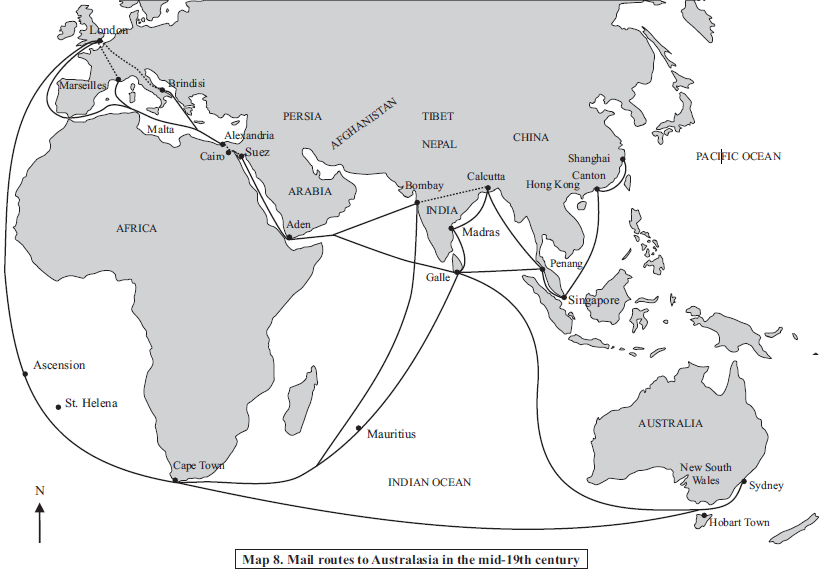
\includegraphics[height=0.95\textheight]{./graphics/NZ/australasian-routes}
\end{figure}
\end{landscape}

\printph{NZ}{PH002}

\printph{NZ}{PH003}

\printph{NZ}{PH004}

\printph{NZ}{PH005}

\printph{NZ}{PH006}

\printph{NZ}{PH007}

\printph{NZ}{PH008}

\printph{NZ}{PH009}

\chapter{Via Suez and Southampton}
\printph{NZ}{PH010}

\printph{NZ}{PH011}

\printph{NZ}{PH012}

\printph{NZ}{PH013}

\printph{NZ}{PH014}

\printph{NZ}{PH015}

\printph{NZ}{PH016}

\printph{NZ}{PH017}

\printph{NZ}{PH018}

\printph{NZ}{PH019}

\section{The Wwreck of the Colombo}
\flushleft
A number of covers have been recovered from the wreck of the Colombo, which was sailing off Minicoy islands in 1862.

The ship sunk in heavy storms outside Minicoy islands in the Indian Ocean. A gravure in the Illustrated London News shows the drama some months after it occurred.

\begin{landscape}
\begin{figure}[p]
\centering
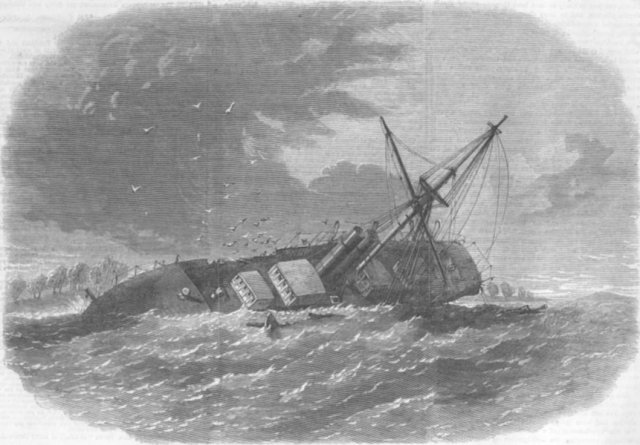
\includegraphics[height=0.9\textheight]{./graphics/NZ/colombo}
\caption{The mail-steamer Colombo wrecked on the North end of Minicoy Island, one of the Laccadives, in the Indian Ocean}
\end{figure}
\end{landscape}


\endflushleft


\printph{NZ}{PH020}


\printph{NZ}{PH021}


\printph{NZ}{PH022}

\printph{NZ}{PH023}

\printph{NZ}{PH024}

\printph{NZ}{PH025}

\printph{NZ}{PH026}

\printph{NZ}{PH027}

\printph{NZ}{PH028}

\printph{NZ}{PH029}


\section{An 8d rate}

\printph{NZ}{PH030}

\printph{NZ}{PH030a}

\printph{NZ}{PH031}

\section{"Express" Route via Marseilles}

\printph{NZ}{PH032}

\printph{NZ}{PH033}

\printph{NZ}{PH034}

\printph{NZ}{PH035}

\printph{NZ}{PH036}

\printph{NZ}{PH037}

\printph{NZ}{PH038}

\printph{NZ}{PH039}

\printph{NZ}{PH040}

\printph{NZ}{PH041}

\printph{NZ}{PH042}

\printph{NZ}{PH043}


\section{Via Brindisi}
\printph{NZ}{PH044}

\printph{NZ}{PH045}

\printph{NZ}{PH046}

\printph{NZ}{PH047}

\printph{NZ}{PH048}

\printph{NZ}{PH049}

\printph{NZ}{PH050}

\printph{NZ}{PH051}

\printph{NZ}{PH052}

\printph{NZ}{PH053}

\printph{NZ}{PH054}

\printph{NZ}{PH055}

\printph{NZ}{PH056}

\section{Non-Contract Ship Letter}
\printph{NZ}{PH057}



\section{The Panama Route}

\printph{NZ}{PH058}

\printph{NZ}{PH059}

\printph{NZ}{PH060}

\printph{NZ}{PH061}

\printph{NZ}{PH062}

\printph{NZ}{PH063}

\printph{NZ}{PH064}

\printph{NZ}{PH065}

\printph{NZ}{PH066}

\printph{NZ}{PH067}

\printph{NZ}{PH068}

\printph{NZ}{PH069}

\chapter{Via Honolulu and San Francisco}
\normalsize

Daily Southern Cross, 4 June\marginnote{Saturday's paper.} 1870. Volume XXVI, Issue 3989, Page 4.
ARRIVAL OF THE WONGA WONGA. The C, N.Z. and A. mail s.s. Wonga Wonga,under the command of T. S. Beale,Esq. , arrived in harbour at an early hour yesterday morning from Sydney, en route for Honolulu. She has about ,60 passengers. Captain Beale reports o£ the passage, as follows : — Left Sydney on Saturday the 28th instant at sp. m. ; rounded the North Cape on the 2nd instant at 1 p.m., and arrived alongside the Queen-street Wharf at 8 o'clock yesterday morning; experienced moderate easterly winds throughout the passage. Passed the s.s. Auckland (also bound here) at 8 p.m. on the 28th. We are indebted to Mr. Robinson, purser, for our files of Australian papers. The s.s. Wonga will take her departure again for Honolulu on Monday next, at 2 p.m.


\printph{NZ}{PH070}

\printph{NZ}{PH071}

\printph{NZ}{PH072}


\printph{NZ}{PH073}

\printph{NZ}{PH074}

\printph{NZ}{PH075}

\printph{NZ}{PH076}

\printph{NZ}{PH077}

\printph{NZ}{PH078}


\chapter{Destination Mail}
\section{European Destinations}

\printph{NZ}{PH079}

\printph{NZ}{PH080}

\printph{NZ}{PH080a}


%includes back-cover
\printph{NZ}{PH081}

\printph{NZ}{PH081a}

\printph{NZ}{PH082}



\printph{NZ}{PH083}




\printph{NZ}{PH084}

\printph{NZ}{PH085}

\printph{NZ}{PH086}

\printph{NZ}{PH086a}

\printph{NZ}{PH087}

\printph{NZ}{PH088}


\printph{NZ}{PH089}

\printph{NZ}{PH090}

\printph{NZ}{PH091}

\printph{NZ}{PH092}

\printph{NZ}{PH093}

\printph{NZ}{PH094}

\printph{NZ}{PH095}

\printph{NZ}{PH096}

\printph{NZ}{PH097}

\printph{NZ}{PH098}

\printph{NZ}{PH098}

\printph{NZ}{PH099}

\printph{NZ}{PH0100}

\printph{NZ}{PH0101}

\printph{NZ}{PH0102}

\printph{NZ}{PH0103}

\printph{NZ}{PH0104}

\printph{NZ}{PH0105}



\printph{NZ}{PH0105}
\chapter{Mail to Australian Colonies}
\section{New South Wales}
\printph{NZ}{PH0106}


\printph{NZ}{PH0107}

\printph{NZ}{PH0108}

\printph{NZ}{PH0109}

\printph{NZ}{PH0110}

\printph{NZ}{PH0111}

\printph{NZ}{PH0112}

\printph{NZ}{PH0113}

\section{Mail to the Australian Colonies, Victoria}

\printph{NZ}{PH0114}

\printph{NZ}{PH0115}

\printph{NZ}{PH0116}

\printph{NZ}{PH0117}

\printph{NZ}{PH0118}

\chapter{Mail to Canada}
\section{Mail to Canada (East)}

\printph{NZ}{PH0118}

\printph{NZ}{PH0119}

\section{Mail to Canada (West)}

\printph{NZ}{PH0120}

\printph{NZ}{PH0121}

\printph{NZ}{PH0122}

\printph{NZ}{PH0123}

\printph{NZ}{PH0124}

\printph{NZ}{PH0125}

\printph{NZ}{PH0126}

\printph{NZ}{PH0127}


\section{Mail to Nova Scotia}


\printph{NZ}{PH0128}

\printph{NZ}{PH0129}

\printph{NZ}{PH0130}

\section{Mail to Canada, Prince Edward Island}

\printph{NZ}{PH0131}


\chapter{Mail to the United States}
\printph{NZ}{PH0132}

\printph{NZ}{PH0133}

\printph{NZ}{PH0134}

\printph{NZ}{PH0135}

\printph{NZ}{PH0136}


\printph{NZ}{PH0137}

\printph{NZ}{PH0138}

\printph{NZ}{PH0139}

\printph{NZ}{PH0140}

\printph{NZ}{PH0141}

\printph{NZ}{PH0142}

\printph{NZ}{PH0143}

\printph{NZ}{PH0144}

\printph{NZ}{PH0145}

\printph{NZ}{PH0146}

\printph{NZ}{PH0147}

\printph{NZ}{PH0148}

\printph{NZ}{PH0149}



\printph{NZ}{PH0150}

\printph{NZ}{PH0151}


\chapter{Mail to the Rest of the World}
\section{Destination Mail, Antiqua}
\printph{NZ}{PH0152}

\section{Destination Mail, Brazil}
\printph{NZ}{PH0153}

\newpage
\section{Cape of Good Hope}
\printph{NZ}{PH0154}

\printph{NZ}{PH0155}


\section{Destination Mail, Ceylon}
\printph{NZ}{PH0156}

\section{Destination Mail, India}
\printph{NZ}{PH0157}

\printph{NZ}{PH0158}

\printph{NZ}{PH0159}

\printph{NZ}{PH0160}

\newpage
\section{Destination Mail, Mauritius}
\printph{NZ}{PH0161}

\printph{NZ}{PH0162}

\section{Destination Mail, New Caledonia}
\printph{NZ}{PH0163}
%\newcounter{counter}
%\setcounter{counter}{84}
%\loop
%\ifnum\value{counter}<92
% \stepcounter{counter}
% \printph{NZ}{PH0\value{counter}}
%\repeat






\appendix

\chapter{Mark Benvie Collection}
\normalsize

New Zealand Mail to Overseas Destinations

The International Large Gold Medal (London 2010)
exhibit formed by Mark Benvie of Auckland

In these days of global tourism and jet airliners, New Zealand is a distant but still accessible destination: in the middle of the 19th century, it was the remotest British Colony on the planet.Posting a letter from New Zealand was much easier said than done.  In the earliest days, mail was placed aboard whatever ship was next leaving harbour.  Letters from “home” arrived infrequently, bringing news that was often a year old when it was received.
The tiny white (almost entirely British) population became accustomed to being an afterthought in the minds of politicians and bureaucrats in London.  There was steady improvement in the postal services between England and the more populous Australian Colonies but New Zealanders could avail themselves of the newer and faster ships only by sending mail to Sydney or Melbourne for on-forwarding to the “Old Country”.

Regular contracted monthly packet services between England and Australia were established only in 1856.  (Even then they were not without their dramas, notably breakdowns and shipwrecks.)  It was only from January 1876 that New Zealand’s overseas mail services could be considered both reliable and enduring.

During the intervening period of just two decades, about a dozen different companies strove valiantly to make a success of providing mail services between Australasia and the rest of the world.  Most of them succumbed to the financial pressures of too little freight and too few paying passengers.  Mail subsidies helped but neither their availability nor their continuance could be relied upon.

The Peninsula \& Orient Line (P\&O) was the most successful of the contractors, but all their voyages from Australia to Europe went via Suez.  Faster connections via North America commenced only in 1866 with a via Panama service.  However, three years and three contractors later, this unprofitable route was abandoned.  For the next six months, New Zealanders were again forced to send their mail via Suez.  A new trans-Pacific service via Honolulu and San Francisco then by rail across America commenced in March 1870 but was interrupted several times over the next five years until more reliable ``permanent'' arrangements were finally made.

Almost by coincidence, the years 1856-75, during which so many developments and dramas occurred on the shipping side of things, roughly mirrored the period during which New Zealand’s classic ``Fullface Queens'' or Chalons were on issue.

First released in 1855, this iconic series appeared on various papers; without or with various watermarks; imperforate, perforated or rouletted.  Stanley Gibbons have assigned 139 whole numbers to the Chalon issue\index{Chalon issue}.

Many prominent philatelists have avidly collected New Zealand’s Chalons.  Famous collections of these enchanting stamps were formed by such luminaries as Alfred Caspary, Maurice Burrus and Alfred Lichtenstein.  In more recent times, the Sir Gawaine Baillie and Joseph Hackmey collections have been added to this pantheon.

However, all of these notable collectors were essentially stamp enthusiasts.  Most of them added covers to their holdings but the emphasis was on usage of the stamps rather than the postal history content.

Mark Benvie, a dedicated postal historian, follows in the footsteps of the eminent New Zealander Gerald Ellott MNZM RDP, whom he acknowledges as both mentor and friend.  It was Ellott who, in the 1980s, produced a monumental three-volumes work on the subject of New Zealand’s postal rates and regulations.  It is Mark Benvie who has built on Ellott’s endeavours, filling in gaps in the recorded knowledge, resolving ambiguities and making a number of important discoveries.

As a postal historian, Mark’s interests have been principally in the routes, rates and markings of the mid-1800s.  The stamps of the period are to him incidental, but included here are many fine and attractive frankings and a number of adhesives rarely seen on cover.

Recognising the importance of provenance, most of Mark’s covers have been sourced from the collections formed by Maurice Burrus, Hugh Gordon Kaye, Marcel Stanley, Royce Bowen (“Yeroc”), John Bishop, Gerald Ellott, Joseph Hackmey, the anonymous “Antipodes”, and the wonderfully eccentric John Woolfe.

The collection encompasses all the overseas routes of the period including an 1856 cover sent via Chile, a swag of scarce via Brindisi items, a scruffy but marvellous cover to Brazil via Panama and London, and the only pre-1875 cover recorded from New Zealand to travel via Trieste See\ref{trieste}.

Unusual rates are revealed, including the first short-lived 9d period to the UK and, most notably, a cover from Timaru posted in the 4-days period when the local newspaper erroneously advised readers of an 8d rate to England.

Mark Benvie was also particularly keen to obtain items to destinations other than Great Britain.  Official Post Office figures reveal that as much as 98\% of all overseas mail from New Zealand was sent to the Australian Colonies (a small proportion) or Britain.  That nearly half the items in this collection are to “other” places speaks of a remarkable achievement.

Included here are covers to Belgium (one recorded), Brazil (the only Chalon cover to anywhere in Latin America), Antigua (one recorded), Ceylon, and the unique cover to New Caledonia carried by a French naval vessel.

Mark Benvie’s efforts to tell the complex story of the evolution of New Zealand’s overseas mails were recognised with a National Gold Medal in New Zealand (2005).  To his delight and surprise, the distinguished jury at London 2010, the world’s most prestigious exhibition, conferred on this collection an International Large Gold Medal.

Since it became known that we would be offering this collection, many clients have expressed surprise that it was coming onto the market.  However, having achieved a Large Gold Medal with a display of only five frames  -  a rare accomplishment indeed  -  Mark considered that, from an exhibiting perspective, he could not take the exhibit further in a way that he would find satisfying.  The rules require that for his next outing he would be required to submit eight frames of material.  To do so would entail a far greater reliance on mail to the UK and would almost inevitably result in significant “padding”.  He simply decided that he didn't want to go down that path.

We at Prestige Philately are proud to present this ``pure'' postal history collection.  We hope that you gain as much enjoyment from studying the catalogue as we have gained from preparing it.


\chapter{SHIPPING DISASTERS}

(From the Times, March l 22.) The opening quarter of the year 1870 will, we fear, be memorable hereafter for a terrible succession of disasters at sea. Of the fate of the City of Boston steamship we would speak with as much uncertainty as we can venture to entertain, for ahe may perhaps still be found afloat ; but the hope is forlorn, and if the apprehensions of the public on both sides of the Atlantic should be, unhappily, realized, the catastrophe will be dreadful indeed. The disappearance of such a vessel, without a single trace of ship, crew, or passengers remaining, would not, it is true, be without precedent, but the precedents are so rare as almost to tell against the supposition. It is nearly thirty years since the President was lost, and since that time only two Atlantic packets have shared a similar fate. 

In 1854 the City of Glasgow, and in 18S6 the Pacific, left port and were never heard of again ; but these, we believe, are the only examples of such losses in the history of Atlantic navigation. In other cases the wreck has been partial, or some have been saved to tell the tale of disaster, and, indeed, the track across the ocean is now so well defined and so incea santly traversed that, except through some overwhelming and instantaneous catastrophe, no vessel could altogether disappear. What may have happened, in the event of the worst, to the City of Boston it would be vain to conjecture. A collision with an iceberg, an overpowering tempest, or a fire on board might be imagined to account for the result ; but the appalling fact would be tjhat a fine, well-found,' and well-msnned steamship had gone to the bottom with every soul on board. Of the wrecks of the Oneida and the Normandy we have more to gay. Of the destructive collision between the Oneida and the Bombay we have received only sufficient information to leave us more perplexed' than before. It seems to be now established that the Bombay did indeed run into the Oneida and cut her down immediately, without slacking her course or stopping to render any assistance to the sinking Teasel. It is alleged, however, on the side of the British vesse), and not disputed so far as we can see by the Americans, that the
collision itself was the fault of the Oneida's pilot. 

The charge against the English commander, is that whereas by timely aid he might probably have saved a hundred lives, he left all these victims to perish without the i slightest heed. His defence is that he neither trie W nor suspected any thing of their, danger. The shock of the collision was so little felt by the Bombay that her captain did not imagine any harm could have been done, and therefore he continued his course. The American version of the occurrence contained statements almost incompatible with such a story. Not only did the Oneida hail the Bombay for assistance, but she blew her whistle as a signal of distress and fired five guns. It is even explained to us how these guns happened to be ready loaded. The Oneida had only left Yokohama two hours before the disaster occurred, and she had expected on going out of port to have to return the salute of a Russian gunboat in the harbour ; but this salute, as it happened, was not given, and so the guns remained loaded. In proof, too, that they were actually fired, it is said the reports vrere heard at Yokohama ; and yet, in contravention of all these assertions, we find, even in the American accounts of the affair, very strange and forcible testimony. When the Bombay arrived at Yokohama, an hour or two afterwards, the proceedings of her Commander, and not only of her Commander, but of her crew and passengers, were entirely consistent with the story afterwards told. Captain Eyre made no report of any collision or accident, nor did he communicate with any of the authorities on the BUbject. Not a word, in short, was known of the affair until fifteen of the survivors landed from the lifeboat the next day, and when they appeared it was as much to the astonishment of the Bombay's crew as to the inhabitants of the place. " 

The passengers," says a New York paper — " the passengers of the Bombay, were quite surprised when they heard the calamity that had befallen the vessel they had struck, but declare they neither heard any request from the Oneida to stay by them or minute guns fired ;" and the report goes on to state that a Naval Court was immediately demanded by the captain of the Bombay, as if in full confidence of his innocence. Of the proceedings and finding of that Court we have already heard something, though not much to our satisfaction. Captain Byre seems to have, been acquitted of blame aa regarded the collision, but his certificate was suspended for six months in consequence of his omission to render assistance to the Oneida's crew. 

By what conclusions the sentence could have been thus measured we are at a loss to understand, but, we presume, the last can hardly have been heard of the affair, and we suspend our judgment. In America the indignation is naturally great, nor can we affect to be surprised at the announcement, made on Saturday by our own correspondent, that " The circumstance that it is an American war- vessel which has been run down, and that the vessel running it down is a British merchant steamer, is an additional cause of bad feeling." That cause of anger, however, will cease, we should hope, on reflection. Even if the nationality of either vessel could alter the complexion of the occurrence, it must be perfectly manifest to the Americans that such nationality could not in the present case have been known or suspected. It is the very essence of Captain Eyre's defence — a defence apparently supported by the unanimous testimony of his passengers — that he hardly knew that he had struck a ship at all, still less that she was an American ship or an American man-of-war. The night was pitch dark, the ships could see nothing of each other but their lights, and though it is lamentable that the British Commander should cot have stopped to see what had been done, or what it behoved him to dp, it is hard to believe that he could have known the truth. The more recent disaster in the Channel is another terrible example of a collision at sea. 

The Normandy was one of the London and South-Western Company's fleet of steamers plying between Southampton and the Channel Islands. 

She was a fine vessel, of nearly 500 tons burden, very fast, and only six years old; and, like the Oueida, she had only* just left port when the disaster occurred. In this case also the night was dark, with a thick fog, and though we do not know at what speed the Normandy was going, we are expressly told that the Mary, a screw steamer of nearly double her tonnage, was going "dead slow, with little or no headway." Nevertheless, when these vessels came into collision the Normandy shared the fate of the Oneida, and was instantly cut down. The Mary, however, did not escape like the \ship{Bombay}. She suffered so terribly from the shock that her safe arrival in port appears miraculous, and yet she seems to have done what she could" for the assistance of the sinking ship. Her boat did not succeed in saving any lives, but she remained on the spot to pick up the boats of the Normandy, and to give what succour could be given. In other respects the similarity between the two stories is remarkable. The collision, the crash, and in ten minutes mere : the final, catastrophe, are described in almost the same words. The loss of life was deplorable ; in fact, the full tale of deaths, if the City of Boston: is to be classed with the Normandy and Oneida, would be almost unexampled. Stormy, too, as the season has been, it was not to the tempest that these wrecks have been due. Possibly the City of Boston perished from stress of weather, but the Oneida and the Normandy went down in smooth with water, without a minute's warning of their peril.

%http://paperspast.natlib.govt.nz/cgi-bin/paperspast?a=d&d=TS18700528.2.12&cl=search&srpos=18&e=--1840---1872--25--1----1Oneida--&st=1


\chapter{Egypt}


\additem{EG}{PH571}%
{Lot No. 571
1733 (May 25): Entire letter from Cairo to Nicholas Caragiani in Venice. A fine and early entire. 80/85}%descrition
{1868}%4
{EG/571}%5
{}%ex
{}
{}%
{}

\additem{EG}{PH572}%
{Lot No. 572
1754 (June 17): Entire letter from Alexandria to Marseille endorsed at lower left "voie de Damiata pour Capt.ne Amiel". Fine and early entire with evidence of disinfection by vinegar splashing on reverse. 100/100}%descrition
{1868}%4
{EG/572}%5
{}%ex
{}
{}%
{}

\additem{EG}{PH573}%
{Lot No. 573
1825 (Feb 20): Entire letter written in French and endorsed at base of letter "au Camp de Kanka" (Tanta), sent to Cairo and endorsed on front panel "Très Pressé". A most unusual usage. 120/260
\index{Camp de Kanka}\index{Tanta}
}%descrition
{1868}%4
{EG/573}%5
{}%ex
{}
{}%
{}

\additem{EG}{PH574}%
{Lot No. 574
Private Couriers 1827 (Aug 28): Entire letter from Damiata to Alexandria with Talismanic Triangle at top and manuscript "Corriere forcato (Forced Courier) che parte alla sera dell'entro sala" at lower left corner. Despite the fact that all letters would have been carried by hand at this date, this letter proves that Couriers operated rather than just house-servants being entrusted with the business or family Mails to carry between towns. A most unusual entire. 200/300 \index{Damiata}}%descrition
{1827}%4
{EG/574}%5
{}%ex
{}
{}%
{}


\additem{EG}{PH575}%
{Lot No. 575
1831 (Feb 15): Entire letter to the Sardinian Consul in Alexandria with manuscript cancellation "Fayoum" at upper left of face panel, the entire toasted for disinfection against Cholera. Rare.240/300
\index{Fayoum}
}%descrition
{1831}%date
{EG/575}%5
{}%ex
{}
{}%
{}

\additem{EG}{PH576}%
{Lot No. 576
1831 (March 18): Entire letter from Alexandrie (Italy) to Alexandria (Egypt), addressed to Sardinian Consul and toasted for disinfection, with fine strikes on front and back of "Lazaretto San / Rococo Di Livorno" in black. Few worm holes on reverse but scarce. \COR2010 100/100}%descrition
{1868}%4
{EG/576}%5
{}%ex
{}
{}%
{}

\additem{EG}{PH577}%
{Lot No. 577
1835 (Aug 18): Entire letter written to the Tuscan Consul in Cairo and endorsed at lower left "Per Espresso" in manuscript. An unusual local usage.}%descrition
{1868}%4
{EG/577}%5
{}%ex
{}
{}%
{}

\additem{EG}{PH578}%
{Lot No. 578
1835: Entire letters (2) from Atfe to Alexandria with Talismanic Triangle at top and manuscript "Retorno del Corriere partito alle 9 AM." . Also a second entire from Atfe to Cairo that shows evidence of being toasted for disinfection. An unusual pair. 240/550}%descrition
{1835}%4
{EG/578}%5
{}%ex
{}
{}%
{}

\additem{EG}{PH579}%
{Lot No. 579
1843 (July 5): Entire letter written in Italian from Tanta to Atfe without postal markings. An unusual cover. 80/120}%descrition
{1868}%4
{EG/579}%5
{}%ex
{}
{}%
{}

\additem{EG}{PH580}%
{Lot No. 580
1846 (Jan 22): Entire letter from Cairo to Khartoum / Sudan addressed in both Arabic and Italian (Carthum), endorsed at base "per mezzo dell' C. R. Nerouni". Extremely rare and very early for in-coming mail to the Sudan.340/1200 }%descrition
{1868}%4
{EG/580}%5
{}%ex
{}
{}%
{}

\additem{EG}{PH581}%
{ Lot No. 581
1851: Entire letter to Cairo, also addressed at top in Arabic, with long letter from Assiout, front panel showing private negative seal handstamp. Scarce and attractive entire. 100/300}%descrition
{1868}%4
{EG/581}%5
{}%ex
{}
{}%
{}

\additem{EG}{PH582}%
{Lot No. 582
1856 (Feb 5): Entire letter from Alexandria to the Sardinian Consul in Cairo, endorsed at upper right "pressé" and struck with extremely fine oval "P.P." in black. Entire with minor imperfections of no real importance compared to the great scarcity of this handstamp. See Smith page 18, fig. 6. Signed Todd. 500/500 }%descrition
{1868}%4
{EG/582}%5
{}%ex
{}
{}%
{}

%\additem{EG}{PH583}%
%{ }%descrition
%{1868}%4
%{EG/583}%5
%{}%ex
%{}
%{}%
%{}


\additem{EG}{PH584}%
{Lot No. 584
1801 (March 5): Entire letter from Siouth datelined 14 Ventose, Year 9; mailed to Cairo and struck with fine strike of "SIOUTH" handstamp in red (23.5x4mm). A rare usage with very few examples recorded. Signed Todd A.I.E.P. and Pothion. Ex collection Antonini. 750 }%descrition
{1868}%4
{EG/584}%5
{}%ex
{}
{}%
{}

\additem{EG}{PH585}%
{Lot No. 585
Napoleonic Occupation 1800: Entire letter addressed to the Commander of the Army of the Orient in Cairo being a translation of a letter from Mourad Bey to General Donzelot from Ghirgeh, mailed to Cairo with manuscript "Siouth" cancellation at upper left. Signed by Donzelot at end of fascinating letter that mentions Jaffa. Rare.300/700 
\index{Napoleonic Occupation! Army of the Orient}
\index{Mourad Bey}
\index{General Donzelot}
}%descrition
{1800}%4
{EG/585}%5
{}%ex
{}
{}%
{}




\additem{EG}{PH586}%
{1831 The Posta Europea system was established in 1824 by an expatriate from Livorno, Michele Pietro Meratti. He owned a small publishing house in Alexandria and had the idea of offering the town residents and merchants a local post service. This idea rapidly expanded into the Posta Europea and a postal service for nearly all lower Egypt. For further reference please see Peter Smith "Egypt-Stamps \& Postal History, a Philatelic Treatise" published by James Bendon in 1999. The following lots are from the collection formed by the late lamented Ambassador Luca Daniele Biolato. 1831 (July 11): Entire letter from the Tuscan Consul in Cairo (cachet on reverse) to the Tuscan Consul in Alexandria, endorsed at top "Con Corriere Europeo" in manuscript. This entire is the earliest recorded item sent by the Meratti Posta Europea, mentioned by Smith on page 15 and illustrated (as are many of the following lots) by Biolato. A wonderful and unique entire for the specialist. SFr750.00/2800.00}%descrition
{1831}%4
{EG/586}%5
{}%ex
{}
{}%
{}



\additem{EG}{PH587}%
{1831 (Sept 28): Entire letter from Alexandria to Livorno, disinfected on arrival in Tuscany with framed "Lazzaretto San / Rocco Di Livorno" cachet in black on reverse, struck with the probably unique impression "POSTA DELLA (?EUROPEA) / M.P.M." (Michele Pietro Meratti). An extraordinary cover that permits unequivocable assignment of this mark to the nascent Merattian Postal Service. Illustrated in Biolato handbook and mentioned by Smith, page 15.2000/5500
\index{Merattian Postal Service}
\index{Meratti, Michele Pietro}
}%descrition
{1831}%4
{EG/587}%5
{}%ex
{}
{}%
{}

\def\CHF#1/#2 {Estimate CHF~#1, Hammer CHF~#2.}

\additem{EG}{PH588}%
{Lot No. 588
1837 (July 26): Entire letter, folded for better display, locally sent within Alexandria and struck with oval italic intaglio seal "... Postale Europea ... Alessandria D'Egitto" in black. An extraordinary and rare cover, mentioned in Smith on page 15.
\COR2010  \CHF750/1300 }%descrition
{1831}%4
{EG/588}%5
{}%ex
{}
{}%
{}

\additem{EG}{PH589}%
{Lot No. 589
1840 (Nov 2): Entire letter from Livorno to Cairo, without postal or rate markings, probably carried from Alexandria by the Meratti Posta Europea with address panel stating "per grazio diretto al Cairo, nello posta del Musco". The Posta Europea P.O. was in the Cairo district of Musky. The Posta Europea service did not introduce either cancellations or rate annotations until the mid 1840's, the receipt of payments made being under subscription from the users of the service. \CHF150/170 }%descrition
{1831}%4
{EG/589}%5
{}%ex
{}
{}%
{}

\additem{EG}{PH590}%
{Lot No. 590
1843: "Direzione Della Posta Europea in Alessandria" Postal Notice issued by Tito Chini (Meratti's cousin who took over the Posta Europea on Meratti's death in 1843) announcing the new postal course between Alexandria and Cairo which were made faster (36 hours), with the postal rates noted at base. A rare and appealing document. \CHF120/600 }%descrition
{1831}%4
{EG/590}%5
{}%ex
{}
{}%
{}

\additem{EG}{PH591}%
{Lot No. 591
1857 (June 1): Printed Invoice from Posta Europea for Postal Services including letters from Atfe and Rosetta and costs for Telegrams. A fine and unusual document. \COR2010  \CHF100/650 }%descrition
{1831}%4
{EG/591}%5
{}%ex
{}
{}%
{}

\additem{EG}{PH592}%
{Lot No. 592
1846 (July 18): Entire letter to Cairo struck on despatch with fine "Smyrne / Turquie" datestamp of French P.O. and framed "P.P.", thence mailed via Malta with circular "Purifié Au Lazaret" in black and slitted for disinfection. Oval framed Type I cachet "POSTA EUROPEA / IN ALESSANDRIA D'EGITTO" in black alongside (Smith = 20 points). Reverse with some flap faults and full French P.O. in Alexandria cds (July 31). A scarce entire. \CHF120/190 }%descrition
{1831}%4
{EG/592}%5
{}%ex
{}
{}%
{}

\additem{EG}{PH593}%
{
Lot No. 593
1846: Entire letter from Cairo to Alexandria without notation of rate, superbly struck with Type I oval "AGENZIA DELLA POSTA EUROPEA / IN CAIRO" in blue. Rare Smith = 9 points. \CHF150/unsold }%descrition
{1831}%4
{EG/593}%5
{}%ex
{}
{}%
{}


\additem{EG}{PH594}%
{
Lot No. 594
1845 (Feb 17): Entire letter to Sardinian Consul in Cairo written from Smyrna (Consular cachet on reverse) struck in transit with under-inked Type I "POSTA EUROPEA / ALESSANDRIA D'EGITTO" in black, unusually with rate (3 piastres) applied in manuscript inside the cancellation. Scarce entire. \CHF180/420 }%descrition
{1831}%4
{EG/594}%5
{}%ex
{}
{}%
{}



\additem{EG}{PH595}%
{1845 (March 8): Entire letter to Sardinian Consul in Cairo written from "Larnica, Cipro" (Cyprus), struck in transit with over-inked Type I "POSTA EUROPEA / ALESSANDRIA D'EGITTO" in black, unusually with rate (1½ piastres) applied in manuscript inside the cancellation. Extremely rare entire 
\COR2010 
\CHF750/950 
\index{Larnaca}
}%descrition
{1831}%4
{EG/595}%5
{}%ex
{}
{}%
{}



\additem{EG}{PH596}%
{
Lot No. 596
1845/48: Entire letters (2) to Cairo, earlier one from Genoa and 1848 entire from Livorno, each struck with despatch handstamps in red or black and entering the Posta Europea system via the French P.O. in Alexandria; earlier cover struck with oval framed Type I cachet "POSTA EUROPEA / IN ALESSANDRIA D'EGITTO" in black or blue alongside (Smith = 20 points) for journey to Cairo. A scarce matched pair. \index{Posta Europea!Type I}
\COR2010 \CHF220/220 
}%descrition
{1831}%4
{EG/596}%5
{}%ex
{}
{}%
{}

\additem{EG}{PH597}%
{Lot No. 597
1846: Entire letters (3) all to Cairo showing very fine strikes of Type I oval handstamp "POSTA EUROPEA / ALESSANDRIA D'EGITTO" in black (Smith = 20 points), one with Consular cachet on reverse; dated between March and September 1846. A very scarce group. 
\COR2010 
\CHF240/2200 \index{Posta Europea!Type I}}%descrition
{1831}%4
{EG/597}%5
{}%ex
{}
{}%
{}

\additem{EG}{PH598}%
{Lot No. 598
1848 (May 17): Entire letter from Malta to Cairo, endorsed "Via Alexandria" prepaid 5 d. in red manuscript, struck with "Malta" cds on reverse in black and oval "P-D.". On arrival transferred from French P.O. in Alexandria to the Posta Europea system with oval framed Type I cachet "POSTA EUROPEA / IN ALESSANDRIA D'EGITTO" in blue alongside (Smith = 20 points) for journey to Cairo. A scarce entire that displays well. \CHF150/750 }%descrition
{1848}%4
{EG/598}%5
{}%ex
{}
{}%
{}

\additem{EG}{PH599}%
{Lot No. 599
1849 (July 18): Cover to Malta prepaid '5' pence in red manuscript, struck with superb strike of British P.O. "ALEXANDRIA" datestamp in red with fine "Purifié Au Lazaret / Malte" disinfection cachet in black. Very scarce with all markings on the obverse of the cover. \CHF150/- }%descrition
{1831}%4
{EG/597}%5
{}%ex
{}
{}%
{}


\additem{EG}{PH600}%
{Lot No. 600
1851 (Oct 13): Entire letter prepaid from Genoa to Sardinian Consul in Cairo, despatch cds in red; mailed via French P.O. in Alexandria (Oct 31) cds on reverse. Thence transferred with magnificent strike of Type II oval handstamp "DIREZIONE DELLA POSTA EUROPEA / ALESSANDRIA D'EGITTO" in black. \CHF150/600 }%descrition
{1831}%4
{EG/600}%5
{}%ex
{}
{}%
{}

\additem{EG}{PH601}%
{Lot No. 601
1856 (July 19): Entire letter prepaid from St. Michel to Cairo, despatch cds in black at upper left and reverse with Turin and Genoa transit cds's; mailed via French P.O. in Alexandria (July 31). Thence transferred with fine strike of Type II oval handstamp "DIREZIONE DELLA POSTA EUROPEA / ALESSANDRIA D'EGITTO" in black 

\CHF100/170 \index{Posta Europea!Type II}}%descrition
{1856}%4
{EG/601}%5
{}%ex
{}
{}%
{}

\additem{EG}{PH602}%
{ Lot No. 602
1851 (Jan 2): Entire letter written and dated in Arabic with outstanding strike of Type II oval handstamp "AGENZIA DELLA POSTA EUROPEA / CAIRO" in black. Exceptional quality 
\CHF200/200 
\index{Posta Europea!Type II}}%descrition
{1831}%4
{EG/602}%5
{}%ex
{}
{}%
{}


\additem{EG}{PH603}%
{Lot No. 603
1851 (Feb 4): Combination entire letter to France, struck with superb oval framed Type II handstamp "AGENZIA DELLA POSTA EUROPEA / CAIRO" in black (early usage), thence via French P.O. in Alexandria (Feb 7) and struck with red framed "Paquebots / De La / Méditerranee" (large cartridge). Marseille cds (Feb 16) on reverse of a fine entire. 
\index{Paquebots/De La/Mediterrannee}
\COR2010 
\CHF120/180 }%descrition
{1831}%4
{EG/603}%5
{}%ex
{}
{}%
{}


\additem{EG}{PH604}%
{Lot No. 604
1852 (May 17): Envelope to Eton College, England mailed from Cairo with superb strike of oval Type II "AGENZIA DELLA POSTA EUROPEA / CAIRO" in black on reverse, prepaid via British P.O. (May 21) with smudged strike of rare Crown "PAID AT ALEXANDRIA" in red. Reverse with Malta "Purifié Au Lazaret" disinfection cachet in black. London/Paid red transit on front and Windsor arrival cds (May 31) on reverse of a rare (probably unique) cover. Provenance: Collection Kurt Wolfsbauer. 400/900 }%descrition
{1831}%4
{EG/604}%5
{}%ex
{}
{}%
{}

\additem{EG}{PH605}%
{Lot No. 605
1857 (Feb 3): Entire letter to Sardinian Consul in Alexandria from the Consul in Cairo (cachet on reverse), without manuscript rate, showing fine strike of Type II oval handstamp "AGENZIA DELLA POSTA EUROPEA / CAIRO" \index{Posta Europea!Type II!Cairo}in black, unusually struck on the reverse. 120/unsold }%descrition
{1831}%4
{EG/605}%5
{}%ex
{}
{}%
{}

\additem{EG}{PH606}%
{
Lot No. 606
1857 (Jan 23): Combination cover to France at six times rate, struck with very fine oval framed Type II handstamp "AGENZIA DELLA POSTA EUROPEA / CAIRO" in black, thence via French P.O. in Alexandria (Jan 24) and struck with red framed "Paquebots / De La / Méditerranee" (small cartridge). Marseille and Montpellier cds's (Feb 3) on reverse. 120/130 }%descrition
{1831}%4
{EG/606}%5
{}%ex
{}
{}%
{}

\additem{EG}{PH607}%
{Lot No. 607
1857 (Feb 17): Combination cover to Nice / Sardinia with oval Type II handstamp "AGENZIA DELLA POSTA EUROPEA / CAIRO" in black, franked by France 1853 40 c. orange and 80 c. carmine (2 examples, one just touched at top otherwise all adhesives with four margins) with Alexandrie French P.O. cds adjacent (Feb 21).  Three line "Piroscafi-Postali-Francesi" in red at top and reverse with Genova and Nizza arrival cds. A delightful and rare double rate cover. 750/3000 }%descrition
{1831}%4
{EG/607}%5
{}%ex
{}
{}%
{}

\additem{EG}{PH608}%
{Lot No. 608
1859 (June 4): Entire letter from Suez to Sardinian Consul in Alexandria, mailed via Forwarding Agent with fine oval "T. BALUCCI / CAIRO" cachet in blue; placed into Posta Europea system and struck with fair Type II "Agenzia Della Posta Europea / Alessandria D'Egitto" handstamp (June 6) in black. A most unusual usage. 150 }%descrition
{1831}%4
{EG/608}%5
{}%ex
{}
{}%
{}


\additem{EG}{PH609}%
{Lot No. 609
1860 (March 24): Entire letter to Sardinian Consul in Alexandria from the Consul in Cairo (cachet on reverse), rated 1 1/2 piastres in red manuscript, showing fine strike of Type II oval handstamp "AGENZIA DELLA POSTA EUROPEA / CAIRO" in blue. Small closed tear at top but a fine and scarce entire. 140 }%descrition
{1831}%4
{EG/609}%5
{}%ex
{}
{}%
{}

\additem{EG}{PH610}%
{Lot No. 610
1859 (May 28): Entire letter from Benha to Cairo unusually rated '60' in blue crayon (=1½ piastres) struck with fair only Type III handstamp "POSTA EUROPEA / BENHA" in blue-green. The earliest recorded date of use from Benha. Rare thus Smith = 25 points. 150/260  }%descrition
{1831}%4
{EG/610}%5
{}%ex
{}
{}%
{}


\additem{EG}{PH611}%
{Lot No. 611
1860 (June 8): Entire letter to Alexandria rated 3 piastres in red crayon manuscript, with fine oval Type III handstamp "POSTA EUROPEA / DAMIATA" struck in blue-green, also a cut-out of same handstamp with manuscript date "2.11.57". \CHF100/- 
\index{Posta Europea!Damiata} }%descrition
{1831}%4
{EG/611}%5
{}%ex
{}
{}%
{}

\additem{EG}{PH612}%
{1858/62: Entire letters (2) each showing oval Type III handstamp "POSTA EUROPEA / KAFR ZAJAT", earlier cover with strike in black and the 1862 entire struck in blue, file folds but a good pair. 100 
\index{Posta Europea!Kafr Zajat}
 }%descrition
{1831}%4
{EG/612}%5
{}%ex
{}
{}%
{}

\additem{EG}{PH613}%
{1856 (Nov 29): Entire letter, some file folds, mailed to Sardinian Consul in Cairo, rated 3 piastres in red crayon manuscript, struck with Type III "POSTA EUROPEA / MANSURA" oval in green and dated in manuscript (and on letter inside). The earliest recorded date of use of this handstamp from Mansura and, indeed, the earliest of any Type III handstamp. Rare thus. Signed Todd. 150/280  
\index{Posta Europea!Mansura}
}%descrition
{1831}%4
{EG/613}%5
{}%ex
{}
{}%
{}

\additem{EG}{PH614}%
{Lot No. 614
1857 (July 22): Entire letter from Nahman Brothers in Alexandria, mailed to Marseille and sent via Forwarding Agent with blue cachet "VARDOCCA \& NIPOTH / TRIESTE" in blue, Trieste cds in black and arrival (Aug 2) on reverse.120/150  }%descrition
{1831}%4
{EG/614}%5
{}%ex
{}
{}%
{}

\additem{EG}{PH615}%
{Lot No. 615
1860: Cover to Mansura rated 1 piastre in blue crayon, struck with fine oval Type III handstamp "POSTA EUROPEA / MEHALLA" in bright blue, dated in handstamp "31.3.60". Unusual usage outside of Cairo or Alexandria. 80/130  }%descrition
{1831}%4
{EG/615}%5
{}%ex
{}
{}%
{}


\additem{EG}{PH616}%
{Lot No. 616
1859 (June 26): Combination entire letter from Mehalla to Paris with rare usage of Type III oval "POSTA EUROPEA / MEHALLA" despatch in blue-green and manuscript rate of 1 piastre in red crayon, thence via French P.O. in Alexandria (June 28) and franked by1853 10 c. bistre and discoloured 40 c. orange tied by 3704 petit chiffres. Reverse with Paris cds (July 7) of receipt. A few small imperfections but an extremely rare item of Egyptian Postal History, it is believed that only two combinations with a Type III Posta Europea cancellation exist. 
\CHF2200/-  
\index{Posta Europea!Mehalla}
\index{Posta Europea!Type III}
}%descrition
{1859}%4
{EG/616}%5
{}%ex
{}
{}%
{}

\additem{EG}{PH617}%
{Lot No. 617
1862 (Dec 17): Entire letter to Alexandria rated 1½ piastres in blue crayon, struck with fine oval Type III handstamp "POSTA EUROPEA / MEHALLA" in blue-green. 80  }%descrition
{1831}%4
{EG/617}%5
{}%ex
{}
{}%
{}


\additem{EG}{PH618}%
{
Lot No. 618
1858 (May 30): Entire letter to Alexandria rated $1\frac{1}{2}$ piastres in red manuscript, struck with oval Type III handstamp "POSTA EUROPEA / SAMANUD" in black. Rare thus-this handstamp almost universally found struck in blue green. 
\COR2010  \CHF120/-   
\index{Posta Europea!Samanud}
}%descrition
{1858}%4
{EG/618}%5
{}%ex
{}
{}%
{}

\additem{EG}{PH619}%
{
\textbf{Fig.\thinspace 619}\sidenote{\textbf{1862 POSTA EUROPEA SUEZ}}
1862 (Sept 8): Entire letter to the Italian Consul in Cairo rated 2 piastres in blue crayon manuscript, struck with an outstanding impression of oval Type III handstamp "POSTA EUROPEA / SUEZ" in blue-green and dated within handstamp in ink. An extremely rare marking in the finest quality. Signed Todd Smith = 24 points. 
\COR2010 
\CHF1200/-  
\index{Posta Europea! Suez}
}%descrition
{1862}%4
{EG/619}%5
{}%ex
{}
{}%
{}

\additem{EG}{PH620}%
{Lot No. 620
1862 (Oct 17): Entire letter from Suez to the Sardinian Consul in Cairo without rating but endorsed in blue manuscript crayon "Postage to be Collected" in Italian at top. A most unusual entire letter as Postage from Suez by the Posta Europea system was mandatory (see Smith page 21). Rare. 240  }%descrition
{1862}%4
{EG/620}%5
{}%ex
{}
{}%
{}

\additem{EG}{PH621}%
{Lot No. 621
1856 (June 11 \& July 24): Entire letters (2) from Tanta to Alexandria without Posta Europea handstamp but certainly carried by the Company, each rated "1½" piastres in red crayon. Tanta was supplied with the Type III handstamp, the earliest date of use seen being January 1, 1857. A rare pair of pre-cursors.
\index{Posta Europea!Earliest Recorded!Tanta}
\index{Tanta}
\COR2010
\CHF150/150  }%descrition
{1831}%4
{EG/621}%5
{}%ex
{}
{}%
{}

\additem{EG}{PH622}%
{Lot No. 622
1858 (Sept 17): Entire letter to the Sardinian Consul in Cairo without rating but endorsed in manuscript crayon "Franca" in red, and struck with superb oval Type III handstamp "POSTA EUROPEA / ZAGASIK" in green. Exceptional and most unusual entire.200/200 
\index{Posta Europea!Zagasik}
\index{Zagasik}
}%descrition
{1831}%4
{EG/622}%5
{}%ex
{}
{}%
{}

\additem{EG}{PH623}%
{Lot No. 623
1862 (July 8): Entire letter to the Italian Consul in Cairo struck with fine strike of unlisted straight line "FRANCA" in blue and oval Type III handstamp "POSTA EUROPEA / ZAGASIK" in same colour. Rare and superb entire. Signed Todd. 600/600 }%descrition
{1831}%4
{EG/623}%5
{}%ex
{}
{}%
{}

\additem{EG}{PH624}%
{Lot No. 624
1862 (Sept 1): Entire letter to Alexandria rated 1 1/2 piastre in red manuscript, struck with fine Type III handstamp "POSTA EUROPEA / ZIFTA" in green. 80
\index{Posta Europea!Zifta}
 }%descrition
{1831}%4
{EG/624}%5
{}%ex
{}
{}%
{}

\additem{EG}{PH625}%
{Lot No. 625
1862 (Sept 14): Entire letter to Alexandria rated 1½ piastres in red manuscript, struck with fine oval Type III handstamp "POSTA EUROPEA / ZIFTA" in green. Fresh and fine entire. 80 
\index{Posta Europea!Zifta}
}%descrition
{1831}%4
{EG/625}%5
{}%ex
{}
{}%
{}

\additem{EG}{PH626}%
{Lot No. 626
1861 (Dec 24): Entire letter to Cairo rated 1 piastre in red manuscript, struck with outstanding strike of circular Type IV datestamp "POSTA EUROPEA / ALESSANDRIA" in blue. Smith states "Types IV and VI are commonly poorly struck..". Exceptional example of this cancellation. 100/150
\index{Posta Europea!Type IV!ALESSANDRIA}
}%descrition
{1831}%4
{EG/626}%5
{}%ex
{}
{}%
{}

\additem{EG}{PH627}%
{
Lot No. 627
1861/62: Entire letters (3) to Cairo all rated 1 piastre in red or blue manuscript, all struck with fair to fine strikes of circular Type IV datestamp "POSTA EUROPEA / ALESSANDRIA" in black (early usage on Jan 25, 1861), in bright blue (Dec 31, 1861) and in blue-green (June 18, 1862). A fine and scarce trio. 150 }%descrition
{1831}%4
{EG/627}%5
{}%ex
{}
{}%
{}

\additem{EG}{PH628}%
{Lot No. 628
1861 (June 24): Combination cover to Florence with reverse showing fine strike of circular Type IV datestamp "POSTA EUROPEA / CAIRO" in black, transferred to French P.O. in Alexandria and franked by 1853 80 c. carmine tied by 3704 petit chiffres and manuscript ink line denoting full pre-payment. Reverse with Livorno transit and Firenze arrival cds. 240/300
\index{Posta Europea!Type IV!Cairo}
}%descrition
{1831}%4
{EG/628}%5
{}%ex
{}
{}%
{}

\additem{EG}{PH629}%
{Lot No. 629
1862 (Sept 1): Combination entire letter to Constantinople with Type IV datestamp "POSTA EUROPEA / CAIRO" despatch in black (as usual, relatively faintly struck), transferred to Austrian P.O. and cancelled with "Alexandrien" cds in blue-green. Blue manuscript '30' (soldi) on reverse alongside "Lloyd Agenzie-Costantinopoli" arrival cds (Sept 8). A rare usage.300/480 }%descrition
{1831}%4
{EG/629}%5
{}%ex
{}
{}%
{}

\additem{EG}{PH630}%
{Lot No. 630
1863 (Feb 7): Combination cover to Florence with Type IV datestamp "POSTA EUROPEA / CAIRO" despatch in black (as usual, relatively faintly struck), transferred to French P.O. in Alexandria (same day cds), franked by 1853 80 c. carmine, margin shaved at top but not affecting appearance, tied by smudged 3794 petit chiffres. Framed "Piroscafi-Postali-Francesi" and 'PD' in black alongside. A scarce cover.  240/320 }%descrition
{1831}%4
{EG/630}%5
{}%ex
{}
{}%
{}

\additem{EG}{PH631}%
{Lot No. 631
1863 (June 14): Entire letter rated 1 piastre in blue crayon manuscript, struck with fine circular Type IV datestamp "POSTA EUROPEA / CAIRO" in black. The latest recorded date of use by six days (see Smith page 19). Scarce thus. }%descrition
{1831}%4
{EG/631}%5
{}%ex
{}
{}%
{}

\additem{EG}{PH632}%
{Lot No. 632
1862 (March 1): Entire letter to Cairo with sender's cachet of "Krebser \& Co./Benna-Abussir" in green, rated at Posta Europea tariff of 1½ piastres in blue manuscript; endorsed "Da Samanud". It is interesting to note that Benha was supplied with the Posta Europea Type III cachet (known usage May-Sept 1859) and the Type V cachet (known usage Oct 1863 to March 1865). This entire falls in-between these dates. Slight staining but a rare entire. }%descrition
{1831}%4
{EG/632}%5
{}%ex
{}
{}%
{}

\additem{EG}{PH633}%
{Lot No. 633
1862 (March 21): Entire letter to Cairo with sender's cachet of "Krebser \& Co./Benna-Abussir" in green, rated at Posta Europea tariff of 1½ piastres in red manuscript; endorsed at top "presentemonte in Alessandria" in blue. It is interesting to note that Benha was supplied with the Posta Europea Type III cachet (known usage May-Sept 1859) and the Type V cachet (known usage Oct 1863 to March 1865). This entire falls in-between these dates. Slight stain at top but a rare entire. 165/300 }%descrition
{1831}%4
{EG/633}%5
{}%ex
{}
{}%
{}

\additem{EG}{PH634}%
{Lot No. 634
1864 (Aug 14): Cover to Cairo rated 1 piastre in blue crayon, struck with outstanding impression of the Type V handstamp "POSTA EUROPEA / BENHA" in blue-green. An exquisite cover of great rarity Smith = 24 points. Provenance: Collection Kurt Wolfsbauer. 500/1200 \index{Posta Europea!Benha}}%descrition
{1831}%4
{EG/634}%5
{}%ex
{}
{}%
{}

\additem{EG}{PH635}%
{Lot No. 635
1863 (Dec 17): Entire letter to Alexandria rated 1 piastre in red manuscript crayon, struck with fine oval Type V datestamp "POSTA EUROPEA / DAMANHOUR" in blue-green. A superb entire, the earliest recorded date of use of this rare marking (Smith = 24 points). Signed Todd. Provenance: Collection Kurt Wolfsbauer. 500/2000  
\index{Posta Europea!Damanhour}
}%descrition
{1831}%4
{EG/635}%5
{}%ex
{}
{}%
{}

\additem{EG}{PH636}%
{Lot No. 636
1864 (Sept 10): Entire letter rated 1 piastre in red crayon manuscript, struck with fine oval Type V datestamp "POSTA EUROPEA / KAFER-ZAYAT" in black. Extraordinarily struck on reverse with "ALESSANDRIA D'EGITTO-POSTE ITALIANE" datestamp of the same day. A rare combination cover and the first this describer has recorded. 300
\index{Posta Europea!Kafer-Zayat}
}%descrition
{1831}%4
{EG/636}%5
{}%ex
{}
{}%
{}

\additem{EG}{PH637}%
{Lot No. 637
1864 (April 17): Entire letter, sent registered, with 3 piastre rate shown in blue manuscript, struck with rare single framed "PER CONSEGNA" handstamp denoting registration (the wording of the handstamp type copied from the Tuscany Post Office) and by oval Type V datestamp "POSTA EUROPEA / KAFR-ZAYAT" in blue-green. Faint Alexandria Type VI arrival in black. Smith: "All registered letters are rare ...". 400/unsold
\index{Posta Europea!Kafr-Zayat}
}%descrition
{1831}%4
{EG/637}%5
{}%ex
{}
{}%
{}

\additem{EG}{PH638}%
{Lot No. 638
1863/64: Covers (3) to Alexandria or Cairo, each rated 2 piastres in red or blue manuscript, each showing fine strikes of oval Type V datestamp "POSTA EUROPEA / MANSURA", in blue (Oct 15, 1863), in green (Oct 31, 1863) and in deep blue-black (July 11, 1864); this last cover being of great scarcity struck in this colour. 150 
\index{Posta Europea!Mansura}
}%descrition
{1831}%4
{EG/638}%5
{}%ex
{}
{}%
{}

\additem{EG}{PH639}%
{Lot No. 639
1865 (April 7): "Ricevuta D'Impostazione" form for letter from Mansura to Alexandria with superb strike of oval Type V handstamp "POSTA EUROPEA / MANSURA" in blue. Exceptional and very scarce. Provenance: Collection Kurt Wolfsbauer. 300/460 
\index{Posta Europea!Mansura}
}%descrition
{1831}%4
{EG/639}%5
{}%ex
{}
{}%
{}

\additem{EG}{PH640}%
{Lot No. 640
1864 (Aug 2): Entire letter to Alexandria rated 1 1/2 piastres in blue manuscript, struck with fine oval Type V datestamp "POSTA EUROPEA / MICHALLA" in black. Reverse with Alxandria Type VI arrival in blue. File fold but scarce. 80/80 
\index{Posta Europea!Michalla}
}%descrition
{1831}%4
{EG/640}%5
{}%ex
{}
{}%
{}

\additem{EG}{PH641}%
{Lot No. 641
1863/64: Covers (2) to Alexandria each showing oval Type V datestamps "POSTA EUROPEA / ZAGASIK", the earlier cover with fine strike in blue, the October 1864 showing same datestamp well struck in black. A fine pair. 100 
\index{Posta Europea!Zagasik}
}%descrition
{1831}%4
{EG/641}%5
{}%ex
{}
{}%
{}

\additem{EG}{PH642}%
{Lot No. 642
1864 (Feb 18): Entire letter to Alexandria with manuscript rate 3 piastres in red crayon, struck with very fine Type V "POSTA EUROPEA / ZIFTA" in blue. Faint Type VI arrival cds in black on reverse of an attractive entire. 80 
\index{Posta Europea!Zifta}
}%descrition
{1831}%4
{EG/642}%5
{}%ex
{}
{}%
{}

\additem{EG}{PH643}%
{Lot No. 643
1863 (Sept 4): Combination cover to Cairo, Egypt franked by Sardinia 1855/61 imperforate 40 c. red in a horizontal pair, fine margins all round, one stamp with wax stain; tied by "Genova Uffizio Del Porto" cds's. Carried by French Steamer with large cartridge "Piroscafi-Postali-Italiani" in blue. "Alessandria D'Egitto" cds on reverse and transferred to Posta Europea with Type VI datestamp "POSTA EUROPEA / ALESSANDRIA" in blue and Type VI arrival of Cairo in blue. Central file fold away from adhesives but a dramatic and rare cover. Signed Sorani. 2500/2500 
\index{Posta Europea!Type VI!ALESSANDRIA}
}%descrition
{1831}%4
{EG/643}%5
{}%ex
{}
{}%
{}


\additem{EG}{PH644}%
{Lot No. 644
1864 (Dec 31): Registered cover to Mansura with superb strike of oval "PER CONSEGNA / POSTA EUROPEA ALESSANDRIA" with registration number 6261, rated at 4 piastres in blue manuscript and struck at upper right with Type VI "Posta Europea / Alessandria" datestamp. Reverse with Type V datestamp of Mansura in blue of the same day. A fine and very rare cover. Signed Todd. Provenance: Collection Kurt Wolfsbauer.  500/1000

\index{Posta Europea!Type VI!Alessandria}
\index{Posta Europea!Type V!Mansura}
}%descrition
{1831}%4
{EG/644}%5
{}%ex
{}
{}%
{}



\additem{EG}{PH645}%
{Lot No. 645
1863 (Dec 29): Official entire letter to Cairo with "Reggio / Calabria" despatch cds, mailed via Messina on French Packet with framed "Piroscafi-Postali-Francesi" in black, transferred from Italian P.O. with "Alessandria D'Egitto" cds with circular Type VI datestamp "POSTA EUROPEA / ALESSANDRIA" (Jan 4, 1864) in black on reverse. Entire opens well for Exhibit display, scarce. 120/200}%descrition
{1831}%4
{EG/645}%5
{}%ex
{}
{}%
{}







\additem{EG}{PH646}%
{Lot No. 646
1864 (Aug 11): Combination entire letter, heavy closed central file fold, mailed from Livorno to Cairo, Egypt with De La Rue 1863 15 c. blue (4 examples) and 60 c. mauve all tied by Livorno cds's, mailed via Italian Steamer with framed small cartridge "Piroscafi-Postali-Italiani" in black. On arrival struck on reverse with "Alessandria D'Egitto" cds (aug 17) and transferred with Type VI datestamp "POSTA EUROPEA / ALESSANDRIA" to Cairo with faint Type VI arrival. Despite faults, a remarkable and extremely rare entire. Cert. Raybaudi (1980). 750/unsold
 }%descrition
{1831}%4
{EG/646}%5
{}%ex
{}
{}%
{}

\additem{EG}{PH647}%
{Lot No. 647
1864 (March 8): Combination cover to Genoa with Type VI datestamp "POSTA EUROPEA / CAIRO" despatch in blue, mailed via Italian P.O. with "Alessandria D'Egitto" cds and franked by 1863 40 c. rose (2 examples, one defective) tied by framed  "Piroscafi-Postali-Francesi" in black. Despite the imperfection, a rare combination usage.  200/440
 }%descrition
{1831}%4
{EG/647}%5
{}%ex
{}
{}%
{}

\additem{EG}{PH648}%
{Lot No. 648
1865 (Jan 13): Combination cover from Cairo re-directed on arrival in Florence to Lisbon / Portugal; envelope struck with Type VI datestamp "POSTA EUROPEA / CAIRO" in black, thence via Italian P.O. in Alexandria where 1863 60 c. mauve was applied and tied by "Alessandria D'Egitto" cds and by framed "Piroscafi-Postali-Italiani" small cartridge handstamp. On arrival in Florence the cover was redirected to Lisbon with 20 c. blue (Type III) tied by manuscript pen cross. Lisbon arrival cds and various transits on reverse of a startling and scarce cover. Cert. La Storia Postale D'Italia (1991). 750/750
 }%descrition
{1831}%4
{EG/648}%5
{}%ex
{}
{}%
{}


\additem{EG}{PH649}%
{Lot No. 649
1860c.: Undated cover to Alexandria addressed to Madam Amabile Carnazzi, sent registered and struck with unlisted type of framed "PER CONSEGNA" handstamp in black. Rare. Provenance: Collection Kurt Wolfsbauer. 500/800
 }%descrition
{1831}%4
{EG/649}%5
{}%ex
{}
{}%
{}


%\additem{EG}{PH650}%
%{
% }%descrition
%{1831}%4
%{EG/650}%5
%{}%ex
%{}
%{}%
%{}



\additem{EG}{PH651}%
{
Lot No. 651
1864: Essays for the Posta Europea Adhesive Stamps The magnificent album page with the four cut square examples for four values as proposed to the Government by \people{Giacomo Muzzi}; lithographed in black on coloured paper inscribed "POSTA EUROPEA / MANSURA": 10 para in yellow, 20 para in blue, 30 para in green and 1 piastre value in white; together with rectangular framed Essays in black on white paper (Piastre Tarifa) "Piast.e Tar.a 1.", "Piast.e Tara.a 1,20", Piast.e Tar.a 2." and "Piast.e Tar.a 3." It is interesting to note that all the values correspond to the rates of the Posta Europea and those of the later Government Post. These Essays were originally found, as offered, glued to the album page and consequently suffer from small faults of negligible importance due to their rarity: of the coloured Essays only two sets of the four values were recorded prior to this (one ex Dr. W. Byam, one ex King Farouk) and of the value only Essays only one other set has been recorded, again ex King Farouk. See Smith pages 22-23. Nile Post E1-E4 and unlisted. Cert. Todd AIEP (2003).5000/8000 }%descrition
{1831}%4
{EG/651}%5
{}%ex
{}
{}%
{}


\additem{EG}{PH652}%
{Lot No. 652
Interpostal Seals 1864/65: Introduced originally by the Posta Europea, these seals are still controversial with this describer believing them to be reseal labels applied to damaged letters and also applied to the top of a bundle of correspondence or parcel, which was tied with string and then the Interpostal applied as a seal. Seven different examples of the scarce first issue with fine to fair mint examples from Benha, Birket-El-Sab, Damiata, Samanud, Tauta, Zagasik and Zifta. 300
 }%descrition
{1831}%4
{EG/652}%5
{}%ex
{}
{}%
{}

\additem{EG}{PH654}%
{Lot No. 654
1865 (July 2): Cover to Mansura rated '2' piastres in manuscript, struck with fine "Poste Vice-Reali Egiziane / Cairo" datestamp in blue, reverse with Mansura arrival (3/7), also in blue. Crossed by file fold but fresh and fine, a scarce cover. 120
 }%descrition
{1831}%4
{EG/654}%5
{}%ex
{}
{}%
{}


\additem{EG}{PH655}%
{Lot No. 655
1865 (Dec 19): "Bolletta Di Deposito" receipt form in Italian for a registered letter, signed by Postal Official 'Lucas' with very fine strike of "Poste Vice-Reali Egiziane / Cairo" cds in black. Creased as usual but very fine and scarce piece. Provenance: Collection Kurt Wolfsbauer.
\index{Deposit notice}
 }%descrition
{1831}%4
{EG/655}%5
{}%ex
{}
{}%
{}

%% FELDMANS 2011 May
%% Syros Greek Post Office
\additem{EG}{PH20058}%
{1870 (Jan 25) Cover from Syros, Greece, to Port Said via the Greek PO at Alexandria, with 40L Large Hermes Head tied by "67" dotted lozenge paying the rate to Alexandria, with both Greek and Egyptian PO transits, and taxed 2pi to Port Said, with arrival bs, minor foxing
\euro 700 
\index{Syros}
 }%descrition
{1870}%4
{EG/20058}%5
{}%ex
{}
{}%
{}


\additem{EG}{PH656}%
{Lot No. 656
1865: Essays by Prevost, 10 pa. in turquoise blue on thick card and 10 pa. Essay in deep blue-green on thick card overprinted 20 paras in black. A fine and scarce pair Nile Post E6f + E7 = \$ 275.  \COR2010  120/240
\index{Prevost Essays}
}%descrition
{1831}%4
{EG/656}%5
{}%ex
{}
{}%
{}


\additem{EG}{PH657}%
{Lot No. 657
1865: Essay by Prevost, square 10 pa. vignette in gold on thick card paper, overprinted 20 paras in black. Rare Nile Post E7 = \$ 135. 
\COR2010  150/160 
\index{Prevost Essay}
}%descrition
{1865}%4
{EG/657}%5
{}%ex
{}
{}%
{}


\additem{EG}{PH658}%
{Lot No. 658
1865: Prevost Essays for the first issue, square 10 para Essays in black (3) with circular framed overprint for 1 piastre at left, on green paper, rose-pink paper and on white. Green example with slight bend, otherwise a fine and very scarce group Nile Post E9a+E9b+E9c = \$ 300 160/280}%descrition
{1831}%4
{EG/658}%5
{}%ex
{}
{}%
{}

\additem{EG}{PH659}%
{Lot No. 659
1865: Prevost Essay for first issue, grey envelope with square 10 pa. vignette in green at left with circular 1 piatre overprint below in same colour. Some minor faults but an attractive and rare envelope Nile Post E9g = \$ 150. 100/140
}%descrition
{1831}%4
{EG/659}%5
{}%ex
{}
{}%
{}

\additem{EG}{PH660}%
{Lot No. 660
1866: Essays by Reister of Paris, the complete set of four Essays without value tablet and with full ornamentation above, in blue, brown, green and red. Superb and very scarce set, undoubtedly made for the proposed second issue with the rectangular design measuring the same size as the issued 1867 adhesives Nile Post E21 = \$500. 280/300

\index{Riester Essays}
}%descrition
{1831}%4
{EG/659}%5
{}%ex
{}
{}%
{}

\additem{EG}{PH661}%
{Lot No. 661
1869: Essay by Prevost "00" para value in black on thin yellow paper with "Epreuve" below and 20 paras overprint in circle at right Nile Post E38 = \$ 75. 60/100
}%descrition
{1831}%4
{EG/661}%5
{}%ex
{}
{}%
{}

\additem{EG}{PH662}%
{Lot No. 662
1867: National Bank Note Company of New York, 20 pa. blue Essay on thick card, slightly cut-down at sides, fresh and fine Essay. Cert. Holcombe (1983) Nile Post = \$ 200. 100/320
\index{National Bank Note Company}
}%descrition
{1831}%4
{EG/662}%5
{}%ex
{}
{}%
{}

\additem{EG}{PH663}%
{Lot No. 663
1867: National Bank Note Company of New York, white envelope with 1 pi. deep green Essay at upper right corner, some minor bends bu a fine and scarce Essay Nile Post E34a = \$ 275. 140/260
}%descrition
{1831}%4
{EG/663}%5
{}%ex
{}
{}%
{}

\additem{EG}{PH664}%
{Lot No. 664
1870: Essay by Reister of Paris, lithographed 20 Para Essay on white wove paper, showing the two types printed in pale khaki-brown in a block of four, overprinted in black; large margins all round. Exceptional and very scarce Nile Post E48 = \$ 350. 200/380
\index{Resiter of Paris}
}%descrition
{1831}%4
{EG/664}%5
{}%ex
{}
{}%
{}

\additem{EG}{PH665}%
{Lot No. 665
1870: Essay by Reister of Paris, lithographed 20 Para Essay on white wove paper, showing the two types printed in pale green in a block of four, overprinted in black. Exceptional and very scarce Nile Post E48 = \$ 350. 180/400
}%descrition
{1831}%4
{EG/665}%5
{}%ex
{}
{}%
{}

\additem{EG}{PH666}%
{Lot No. 666
1869: Prevost Postal Stationery Essay "Epreuve / 00 Para" in brown on green laid paper envelope. A fresh and fine example. Scarce. Opinion Holcombe (1983) Zeheri 29/IB/Nile Post E36b. 

\CHF150/160 
}%descrition
{1831}%4
{EG/666}%5
{}%ex
{}
{}%
{}

\additem{EG}{PH667}%
{Lot No. 667
1865/66: Pellas Proofs for the first issue, imperforate on unwatermarked white wove paper, a fresh and fine complete set of seven. 100/200
\index{Pellas Proofs}
}%descrition
{1831}%4
{EG/667}%5
{}%ex
{}
{}%
{}

\additem{EG}{PH668}%
{Lot No. 668
20 pa. blue, wmk. upright, Type II, a fine unused example perf 12 1/2 x 13 x imperf. x 13. A scarce stamp Gi = £ 100+. 60/unsold
}%descrition
{1831}%4
{EG/668}%5
{}%ex
{}
{}%
{}

\additem{EG}{PH669}%
{Lot No. 669
1866 (Jan 10): 20 para blue, a superb horizontal pair used on 1866 entire letter within Alexandria, neatly tied by 'retta' 81 dot cancellation well struck in black. "Poste Vice-Reali Egiziane-Alessandria" cds below dated January 10th, 1866 in black. Slightest of file folds at right in no way affecting the delightful appearance, with gold dusted address. A rare cover demonstrating a very fine early usage on the tenth day of issue. Signed Todd A.I.E.P. Provenance: Corinphila sale 118, October 1999, lot 7878. 1000/3400
\index{retta}
}%descrition
{1831}%4
{EG/669}%5
{}%ex
{}
{}%
{}

\additem{EG}{PH670}%
{Lot No. 670
1 pi. claret, a vertical mint strip of three (Types II-I-I), perf 12 1/2 x imperforate between horizontally, top stamp showing plate flaw with "comma for stop between PE" at lower right corner, a fresh and very fine multiple with large part original gum. Rare. Certificate RPS (1971) Gi = £ 400+ 340/400
}%descrition
{1831}%4
{EG/670}%5
{}%ex
{}
{}%
{}


\additem{EG}{PH671}%
{Lot No. 671
1 pi. claret, perf. 13 all round (Type II), fine mint example, couple of blunted perfs. but with fine, large part original gum. A very scarce stamp Gi = £ 300. 140/340
}%descrition
{1831}%4
{EG/671}%5
{}%ex
{}
{}%
{}

\additem{EG}{PH672}%
{Lot No. 672
1 pi. claret, fine example used on 1866 cover to Alexandria cancelled by "Poste Vice-Reali Egiziane / Cairo" cds (March 12) in black. Arrival cds on reverse of attractive cover. Signed Darteyre and Todd.100/100
}%descrition
{1831}%4
{EG/672}%5
{}%ex
{}
{}%
{}

\additem{EG}{PH673}%
{Lot No. 673
1 pi. claret, fine example, perf. 13 on one side, used on 1867 cover to Cairo cancelled by "Poste Vice-Reali Egiziane / Alessandria" cds (Feb 9) in black., arrival cds on reverse. Signed Todd.
}%descrition
{1831}%4
{EG/673}%5
{}%ex
{}
{}%
{}

\additem{EG}{PH674}%
{Lot No. 674
2 pi. bright yellow, Proof block of six without watermark, perf. 12 1/2 x 13, of fine frontal appearance but with some toning on reverse. A scarce multiple. 150/150
}%descrition
{1831}%4
{EG/674}%5
{}%ex
{}
{}%
{}


\additem{EG}{PH675}%
{Lot No. 675
2 pi. yellow, perf. 12 1/2 x 15, a very fine unused example showing the "thin" overprint (see Smith page 144). Very scarce and under-catalogued stamp Gi = £ 130. 80/80
}%descrition
{1831}%4
{EG/675}%5
{}%ex
{}
{}%
{}


\additem{EG}{PH676}%
{Lot No. 676
5 pi. rose, wmk. inverted, Type I, an imperforate example, slight thin and part original browned gum Nile Post D6z = \$ 400. 150
}%descrition
{1831}%4
{EG/676}%5
{}%ex
{}
{}%
{}


\additem{EG}{PH677}%
{Lot No. 677
5 pi. rose, wmk. upright, Type II, perf. 13 x 12 1/2 x 13 x 12 1/2, fine colour, fresh and fine unused. A delightfully centred example of this scarce stamp Nile Post D6n = \$ 450/Gi = £ 275. 160/180
}%descrition
{1831}%4
{EG/677}%5
{}%ex
{}
{}%
{}

\additem{EG}{PH678}%
{Lot No. 678
5 pi deep rose, imperforate Proof example showing Error of Surcharge "10 pi. for 5 pi." at base of overprint, large margins all round, no watermark, unused. A scarce Proof. 200/220
}%descrition
{1831}%4
{EG/678}%5
{}%ex
{}
{}%
{}

\additem{EG}{PH679}%
{Lot No. 679
10 pi. slate, unwatermarked Proof block of six, marginal (Types II-II/II-II/I-I), perf. 13 all round. Unused block with some overall toning but scarce. 100/150
}%descrition
{1831}%4
{EG/679}%5
{}%ex
{}
{}%
{}

\additem{EG}{PH681}%
{Lot No. 681
1869: Essays by Renard of Paris,\index{Essays!Renard of Paris} four examples in different colours: gold, carmine, green and orange-yellow; all overprinted in black (similar to first issue) with 20 paras in black. Narrow margins as usual and one or two imperfections but rare Nile Post E44 = \$ 1'600. 500/1000
\index{Renard of Paris}
}%descrition
{1831}%4
{EG/681}%5
{}%ex
{}
{}%
{}

\additem{EG}{PH682}%
{Lot No. 682
1871 (Dec 25): Small piece of "La Trombetta"\index{Newspapers!La Trombetta} Newspaper (No. 661) bearing diagonally bisected 1867 10 pa. lilac tied by "V. R. Poste Egiziane / Alessandria" cds (signed Todd), together with the complete original Newspaper (No. 661) with vandalized bisect Gi = £ 750. 340/1200
\index{Newspapers!La Trombetta}
}%descrition
{1831}%4
{EG/682}%5
{}%ex
{}
{}%
{}

\additem{EG}{PH683}%
{Lot No. 683
1868 (Dec 19): Entire letter from Cairo to Florence with delightful three colour franking paying the 3 1/2 piastre rate, with 1867 20 pa. green, 1 pi. red and 2 pi. deep blue tied by "PVRE-Cairo" datestamps in black. Italic "Franca" alongside and reverse with Alexandria, Trieste, Venice (Xmas Day) and Florence datestamps. Minor ageing on perforations but a remarkably rare and attractive cover. 1000/3200
}%descrition
{1868}%4
{EG/683}%5
{}%ex
{}
{}%
{}

\additem{EG}{PH685}%
{Lot No. 685
Combination cover (1868) to Livorno franked by Egypt 1867 1 pi. red tied by 'PVRE-Cairo' cds in black, transferred to Italian P.O. and franked by 1863 60 c. bright mauve (Sassone T21) tied by '234' lozenge of dots. Thence via Italian Steamer via Brindisi and struck with small cartridge "Piroscafi-Postali-Italiani" in black. Livorno arrival cds on reverse (March 7). Horizontal file fold away from adhesives, a fine and scarce cover. Cert. Sorani (1992). 1000/unsold
}%descrition
{1868}%4
{EG/685}%5
{}%ex
{}
{}%
{}

\additem{EG}{PH686}%
{Lot No. 686
2 pi. bright blue, imperforate block of four on watermarked paper (upright), Types I-II/III-IV, fresh and fine unused. Only one sheet found, a rare and attractive block Nile Post D12h = \$ 1'000. 500
}%descrition
{1868}%4
{EG/686}%5
{}%ex
{}
{}%
{}


\additem{EG}{PH688}%
{Lot No. 688
1871: Essays by Penasson of Alexandria, 1 pi. values (2) printed in orange, one perforated 12 1/2, the other imperforate. A fine and scarce pair.
\index{Penasson of Alexandria}
\index{Esays!Pennasson}
}%descrition
{1868}%4
{EG/688}%5
{}%ex
{}
{}%
{}


\additem{EG}{PH689}%
{Lot No. 689
1871: Essays by Penasson of Alexandria, the fine group of imperforate Essays without inscription or values, with Pyramid \& Sphinx design, imperforate on wove paper in grey-green, violet, green, red, grey-lilac and orange 6); also a perforated example in blue Nile Post E51 = \$ 450+.

\COR2010 
\CHF200/320 

}%descrition
{1868}%4
{EG/689}%5
{}%ex
{}
{}%
{}


\additem{EG}{PH690}%
{Lot No. 690
Lithographed 20 pa. blue, perf. 12 1/2, well centred unused example of good colour. Signed Todd and Brun Gi = \pounds{120}.
60/90 
}%descrition
{1868}%4
{EG/690}%5
{}%ex
{}
{}%
{}


\additem{EG}{PH691}%
{Lot No. 691
5 para brown (2 + a vertical pair) and 1 piastre red used on attractive 1876 envelope to Dresden, tied with black arabic "POSTE EGIZIANE ASSUAN" (Feb 9) cds, thence via Siut and Alexandria (Feb 16). Dresden arrival cds on reverse of an outstanding cover. 2500/2500
}%descrition
{1868}%4
{EG/691}%5
{}%ex
{}
{}%
{}

\additem{EG}{PH692}%
{Lot No. 692
Typographed 20 pa. blue, perf. 12 1/2 x 13 1/2, a superb and fresh mint block of twelve, fine large part og. A delightful and rare multiple Gi = £ 780+. 500/1400
}%descrition
{1868}%4
{EG/692}%5
{}%ex
{}
{}%
{}


\additem{EG}{PH693}%
{Lot No. 693
1874 (Oct 24): Cover from Cairo to Vienna franked by 1872 typographed 20 pa. blue and 2 pi. yellow, perf 13 1/4, tied by neat Cairo cds in black. Repeated strike below and framed "PD" adjacent. Backstamped at Alexandria, Brindisi and Vienna (Nov 1). A delightful and scarce cover. Signed Todd. 300/380
}%descrition
{1868}%4
{EG/693}%5
{}%ex
{}
{}%
{}


\additem{EG}{PH694}%
{Lot No. 694
2 pi. yellow, good used example cancelled with clear strike of "GEDDA" datestamp in black (March 1873). 80/100
\index{Gedda}
}%descrition
{1868}%4
{EG/694}%5
{}%ex
{}
{}%
{}

\additem{EG}{PH695}%
{Lot No. 695
1874 (Oct 18): Dramatic four colour franking cover from Cairo "Via Brindisi" to Menziken/Switzerland bearing 1872 5 pa. brown, 10 pa. mauve, 20 pa. deep blue and 2 pi. yellow all tied by "Poste Egiziane / cairo" cds's in black. Framed "P.D." on front and reverse with Egyptian P.O. Alexandria transit, Brindisi transit (Oct 22) and Menziken arrival cds (Oct 24). A famous and wonderful cover. Signed Todd A.I.E.P. Provenance: Collection "Cihangir", Corinphila, lot 2525, May 2000. Provenance: Collection Silvain Wyler. 5000/5000
\index{Cihangir}
\index{Frankings!Four colour}
}%descrition
{1868}%4
{EG/695}%5
{}%ex
{}
{}%
{}


%\additem{EG}{PH696}%
%{
%}%descrition
%{1868}%4
%{EG/696}%5
%{}%ex
%{}
%{}%
%{}

\additem{EG}{PH697}%
{Lot No. 697
1873 (Jan 1): Postal Notice headed "Administrazione Delle Poste Khedevie Egiziane / Avviso" printed in Italian and Arabic stating that, from January 1st 1873, due to a new Postal Convention being signed with Italy, that "francobolli egiziani" would alone be necessary. A fine album page size document, attractive and very unusual. 240/700

\index{Postal Notice}
}%descrition
{1868}%4
{EG/697}%5
{}%ex
{}
{}%
{}

\additem{EG}{PH698}%
{Lot No. 698
Bulaq 5 pa. brown, the superb mint foliate marginal block of four showing two vertical tête-bêche pairs, positions 5-6/15-16, fresh and fine, large part og. Certificate Egypt Study Circle (1980) Gi = £ 70+. 80/120
}%descrition
{1868}%4
{EG/698}%5
{}%ex
{}
{}%
{}

\additem{EG}{PH699}%
{Lot No. 699
Bulaq 10 pa. grey lilac, a fine mint vertical tête-bêche pair, foliate marginal, fresh and fine, minor thin on one stamp, large part og. An extremely attractive pair Gi = £ 140. 100/160
}%descrition
{1868}%4
{EG/699}%5
{}%ex
{}
{}%
{}

\additem{EG}{PH700}%
{Lot No. 700
Bulaq 10 pa. grey lilac, a superb mint block of nine, showing central stamp tête-bêche. Superb large part original gum, a fine and rare block Gi = unpriced. 300/480
}%descrition
{1868}%4
{EG/700}%5
{}%ex
{}
{}%
{}

\additem{EG}{PH701}%
{Lot No. 701
Bulaq 1 pi. red, perf. 12 1/2, delightful mint block of six with full foliate margin, showing three vertical tête-bêche pairs (positions 5-7/15-17). Rich colour and superb og., a lovely block Gi = £ 270+. 300/360
}%descrition
{1868}%4
{EG/701}%5
{}%ex
{}
{}%
{}

\additem{EG}{PH702}%
{Lot No. 702
Bulaq 1 pi. red, crossed by file fold, used on 1877 cover to Cairo cancelled by two very fine strikes of  "Poste Egiziane / Suez" datestamps (May 10) with "V.R." removed. Rare. 100/100
}%descrition
{1868}%4
{EG/702}%5
{}%ex
{}
{}%
{}

\additem{EG}{PH703}%
{Lot No. 703
Bulaq 2 1/2 pi. violet, the mint block of four showing tête-bêche pair, fresh and fine, large part og Gi = £ 350+. 180/320
}%descrition
{1868}%4
{EG/703}%5
{}%ex
{}
{}%
{}

\additem{EG}{PH704}%
{Lot No. 704
Bulaq 1 pi. red, perf. 12 1/2, in a very fine mint foliate corner marginal vertical tête-bêche pair, 1 pi. red single frankings on covers (6) from Alexandria, Cairo and Suez. 120/260
}%descrition
{1868}%4
{EG/704}%5
{}%ex
{}
{}%
{}

\additem{EG}{PH705}%
{1879c.: Proof of the "Star \& Crescent" watermarked paper, with nine positions of the watermark and showing marginal rule at upper right. An unusual piece. 120/160
}%descrition
{1868}%4
{EG/705}%5
{}%ex
{}
{}%
{}




\additem{EG}{PH706}%
{Lot No. 706
1879/88: De La Rue Die Proofs (2) imperforate on very thick card for 1879 1 pi. value in black and 1888  5m. in black. Scarce and fine. 120/120
}%descrition
{1868}%4
{EG/706}%5
{}%ex
{}
{}%
{}




\additem{EG}{PH707}%
{Lot No. 707
1879/81: Imperforate Proofs (7) on watermarked gummed paper in issued colours for the complete 1879 issue: 5 pa. brown, 10 pa. reddish lilac, 10 pa. in claret (issued in 1881), 20 pa. pale blue, 1 pi. rose, 22 pi. orange and 5 pi. green; five with part of Plate number in margin at right. Rare and very attractive set Nile Post = \$ 1'200. Provenance: Collection Danson, lot 266 (1977). 
\index{Danson}
\COR2010 
\CHF500/2800 
}%descrition
{1868}%4
{EG/707}%5
{}%ex
{}
{}%
{}

\additem{EG}{PH708}%
{Lot No. 708
1879: De La Rue definitive set of six values, all in fresh mint marginal or corner blocks of four, most stamps unmounted og. A fine and scarce set Gi = £ 900+. 100/130
}%descrition
{1868}%4
{EG/708}%5
{}%ex
{}
{}%
{}

\additem{EG}{PH709}%
{Lot No. 709
1881: 10 pa. claret, the superb mint marginal block of four, wmk. inverted, fresh colour, unmounted og. Scarce Gi = £ 200. 100/130
}%descrition
{1868}%4
{EG/709}%5
{}%ex
{}
{}%
{}

\additem{EG}{PH710}%
{Lot No. 710
1891: De La Rue Die Proof for 3 m. value struck in black on glazed white card, handstamped "BEFORE HARDENING" in black and dated "1 MAY 1891" in blue at left. A fine and scarce Proof. Opinion Holcombe. 150/340
}%descrition
{1868}%4
{EG/710}%5
{}%ex
{}
{}%
{}

\additem{EG}{PH711}%
{
Lot No. 711
1895: Prepared for use by De La Rue in London but unissued, the Winter Fair set of three values: 3 m. orange-yellow, 5 m. rose carmine and 1 pi. blue, fresh and fine, large part og Nile Post C1/C3 = \$ 375. 200/260
}%descrition
{1868}%4
{EG/711}%5
{}%ex
{}
{}%
{}

\additem{EG}{PH712}%
{Lot No. 712
1906: Essays by Bradbury Wilkinson \& Co., the set of three proposals with 5 m. Sphinx \& Pyramid imperforate on white paper in black \& green; similar example in black \& ultramarine, and 10 m. black, red \& blue imperforate and applied on thick card - all are perforated "Specimen" at base. A remarkable and very rare group. Cert. Holcombe for 10 m. (1990) Nile Post E142+E143 = \$ 2'050 800/2200
}%descrition
{1868}%4
{EG/712}%5
{}%ex
{}
{}%
{}

\additem{EG}{PH713}%
{Lot No. 713
1906: De La Rue imperforate Proof of 4 m. value printed in purple on yellow imperforate paper, affixed to paper from the DLR Record book with manuscript "3 Aug 1906" alongside in pencil. Rare, in all probability a Proof for the Postal Stationery card and not the adhesive stamp. Rare. 340/1300
}%descrition
{1868}%4
{EG/713}%5
{}%ex
{}
{}%
{}

%\additem{EG}{PH714}%
%{
%Lot No. 714
%1914: Parcel Post Cards used to Switzerland (7) all with 1889/1902 10 pi. mauve used in combination with lower value adhesives, all cancelled by "Douane Alexandrie R.P." datestamps with framed "DRAWBACK" cachet at left and yellow Customs labels on each for export of Tobacco and Cigarettes, all have Trieste transit datestamps and green Swiss Customs cachets of receipt. A scarce group. 200/460
%}%descrition
%{1868}%4
%{EG/714}%5
%{}%ex
%{}
%{}%
%{}

\additem{EG}{PH715}%
{Lot No. 715
1914: Pictorial Issue, imperforate Proof pairs with watermark, the complete set of ten values (incl. additional pair of the 2 m. in differing shade), fresh and fine, unmounted og. Scarce Nile Post D53b/D62a. 200/280
}%descrition
{1868}%4
{EG/715}%5
{}%ex
{}
{}%
{}

\additem{EG}{PH716}%
{Lot No. 716
1921/22: Proof for the 15 m. value, a fine imperforate horizontal pair on thick un-watermarked paper, printed in black. Scarce Nile Post = \$ 350 140/220
}%descrition
{1868}%4
{EG/716}%5
{}%ex
{}
{}%
{}

\additem{EG}{PH717}%
{Lot No. 717
1922: Colour Trial for the Monarchy Overprint struck in red on 15 m. indigo, fresh and fine, unmounted og. Only 120 stamps were overprinted thus. Rare and appealing item Nile Post D85ct = \$ 250.
}%descrition 120/120
{1868}%4
{EG/717}%5
{}%ex
{}
{}%
{}

\additem{EG}{PH718}%
{Lot No. 718
1922 (Jan 24): Cover from Gibraltar endorsed at top "Consignee's Letter per S.S.Massilia" mailed with Gibraltar 2 d. grey and Egypt 1921 5 m. pink sharing "Port Said" cds (Feb 4). Reverse with two Gibraltar Company cachets and Cairo arrival. Scarce commercial usage. 100/110
}%descrition
{1868}%4
{EG/718}%5
{}%ex
{}
{}%
{}

\additem{EG}{PH719}%
{Lot No. 719
1933: Aviation Congress, the set of five in mint blocks of four, and a further two sets in mint lower right corner Control A33 pairs, fresh and fine, large part og Gi = £ 300. 140/160
}%descrition
{1868}%4
{EG/719}%5
{}%ex
{}
{}%
{}

\additem{EG}{PH720}%
{Lot No. 720
1927 (Nov 15): Cover to Cairo franked solely by the 1926 Express 20 m. deep green tied by Tanta cds in black, reverse with "Postmen / Cairo" cds of receipt. Framed bilingual "Express" cachet at left. Cover with tears but a rare commercial usage. 80/80
}%descrition
{1868}%4
{EG/720}%5
{}%ex
{}
{}%
{}


\additem{EG}{PH721}%
{Lot No. 721
1934 (Jan 2): Cover to Qena struck with superb impression of the newly introduced Nessim machine Cairo 5 m. Meter marking in red, with Qena arrival cds on reverse. Rare, the machine was withdrawn from use on May 25, 1934. 150/unsold
}%descrition
{1868}%4
{EG/721}%5
{}%ex
{}
{}%
{}

\additem{EG}{PH722}%
{Lot No. 722
1936 (Dec 22): First Day Cover of Anglo-Egyptian Treaty with set of three and additional 5 m., with "Parliament" cds and "British Embassy-Cairo" cachet in violet; signed by Egyptian Prime Minister "Nahas Pasha" and by British negotiator of the Treaty, "Sir Miles Lampson". Rare. 400/unsold
}%descrition
{1868}%4
{EG/722}%5
{}%ex
{}
{}%
{}


\additem{EG}{PH723}%
{Lot No. 723
1957 (Jan 14): Imperforate Proof block of four of the overprint only, bilingual in black, fresh and fine on white card paper. Rare: just 100 examples from two panes exist. Cert. Hass (1997) Nile Post = \$ 480. \CHF240/240 
}%descrition
{1868}%4
{EG/723}%5
{}%ex
{}
{}%
{}




%24-25 bulk lots

%26-30 bulk lots


\additem{EG}{PH730}%
{Lot No. 720
1927 (Nov 15): Cover to Cairo franked solely by the 1926 Express 20 m. deep green tied by Tanta cds in black, reverse with "Postmen / Cairo" cds of receipt. Framed bilingual "Express" cachet at left. Cover with tears but a rare commercial usage. 80/80
}%descrition
{1868}%4
{EG/730}%5
{}%ex
{}
{}%
{}


\additem{EG}{PH731}%
{Lot No. 720
1927 (Nov 15): Cover to Cairo franked solely by the 1926 Express 20 m. deep green tied by Tanta cds in black, reverse with "Postmen / Cairo" cds of receipt. Framed bilingual "Express" cachet at left. Cover with tears but a rare commercial usage. 80/80

\index{Express}
}%descrition
{1868}%4
{EG/731}%5
{}%ex
{}
{}%
{}

\additem{EG}{PH732}%
{Lot No. 720
1927 (Nov 15): Cover to Cairo franked solely by the 1926 Express 20 m. deep green tied by Tanta cds in black, reverse with "Postmen / Cairo" cds of receipt. Framed bilingual "Express" cachet at left. Cover with tears but a rare commercial usage. 80/80
}%descrition
{1868}%4
{EG/732}%5
{}%ex
{}
{}%
{}

\additem{EG}{PH733}%
{Lot No. 720
1927 (Nov 15): Cover to Cairo franked solely by the 1926 Express 20 m. deep green tied by Tanta cds in black, reverse with "Postmen / Cairo" cds of receipt. Framed bilingual "Express" cachet at left. Cover with tears but a rare commercial usage. 80/80
}%descrition
{1868}%4
{EG/733}%5
{}%ex
{}
{}%
{}


\additem{EG}{PH734}%
{Lot No. 720
1927 (Nov 15): Cover to Cairo franked solely by the 1926 Express 20 m. deep green tied by Tanta cds in black, reverse with "Postmen / Cairo" cds of receipt. Framed bilingual "Express" cachet at left. Cover with tears but a rare commercial usage. 80/80
}%descrition
{1868}%4
{EG/734}%5
{}%ex
{}
{}%
{}

\additem{EG}{PH735}%
{Lot No. 720
1927 (Nov 15): Cover to Cairo franked solely by the 1926 Express 20 m. deep green tied by Tanta cds in black, reverse with "Postmen / Cairo" cds of receipt. Framed bilingual "Express" cachet at left. Cover with tears but a rare commercial usage. 80/80
}%descrition
{1868}%4
{EG/735}%5
{}%ex
{}
{}%
{}

\additem{EG}{PH736}%
{Lot No. 736
Essay by Harrisons, 15 m. in red, a top marginal block of four printed on watermarked gummed paper, lotus column design in reduced format. A fresh and fine multiple Nile Post E203c = \$ 200. 120/300
}%descrition
{1868}%4
{EG/736}%5
{}%ex
{}
{}%
{}

\additem{EG}{PH737}%
{Lot No. 737
Essay by Harrisons, 15 m. in red brown, a top marginal block of four printed on watermarked gummed paper, lotus column design in reduced format. A fresh and fine multiple Nile Post E203c = \$ 200. 120/320
}%descrition
{1868}%4
{EG/737}%5
{}%ex
{}
{}%
{}


\additem{EG}{PH738}%
{
Lot No. 738
Essay by Harrisons, 15 m . red-brown in a card paper imperforate block of four with the two designs vertically se-tenant, fresh and very fine Nile Post E203e/204e = \$ 400 150/460
}%descrition
{1868}%4
{EG/738}%5
{}%ex
{}
{}%
{}

\additem{EG}{PH739}%
{Lot No. 739
Essay by Harrisons, 15 m. inoranage-yellow, a lower marginal horizontal pair printed on watermarked gummed paper, design in reduced format, also four further single examples of the lotus column design on gummed paper printed in brown (2, different shades), blue and in red Post E203d+204d = \$ 300. 140/300
}%descrition
{1868}%4
{EG/739}%5
{}%ex
{}
{}%
{}

\additem{EG}{PH740}%
{Lot No. 740
Essay by Harrisons of London, imperforate Essay for proposed 15 m. value, ungummed and unwatermarked, showing the two small format designs se-tenant vertically, lithographically printed in blue. Fresh and very fine Nile Post E204f = \$ 400. 200/480
}%descrition
{1868}%4
{EG/740}%5
{}%ex
{}
{}%
{}


\additem{EG}{PH741}%
{Lot No. 741
Essay by Harrisons, 15 m. red-brown on card paper imperforate block of four, marginal, reduced format with the single (lower part of sheet) design, fresh and very fine Nile Post E204a = \$ 200. 120/300
}%descrition 
{1868}%4
{EG/741}%5
{}%ex
{}
{}%
{}

\additem{EG}{PH742}%
{Lot No. 743
Essay by Harrisons, 15 m. in blue, a corner marginal block of four from upper right of sheet printed on un-watermarked wove paper (not card), large format. A most unusual block Nile Post E204a var = \$ 200. 120/380
}%descrition
{1868}%4
{EG/742}%5
{}%ex
{}
{}%
{}

\additem{EG}{PH743}%
{Lot No. 743
Essay by Harrisons, 15 m. in blue, a corner marginal block of four from upper right of sheet printed on un-watermarked wove paper (not card), large format. A most unusual block Nile Post E204a var = \$ 200. 120/280
}%descrition
{1868}%4
{EG/743}%5
{}%ex
{}
{}%
{}

\additem{EG}{PH744}%
{Lot No. 744
Essay by Harrisons, 5 m. in deep black \& white, imperforate and affixed to card paper, fine and scarce Nile Post E219 = \$ 100+. 100/190
}%descrition
{1868}%4
{EG/744}%5
{}%ex
{}
{}%
{}

\additem{EG}{PH745}%
{Lot No. 745
Essay by Harrisons, 5 m. red brown in a fine perforated 13 3/4 x 14, block of four on watermarked gummed paper Nile Post E227 = \$ 300. 120/300
}%descrition
{1868}%4
{EG/745}%5
{}%ex
{}
{}%
{}

\additem{EG}{PH746}%
{Lot No. 746
Essay by Harrisons, engraved Essay for 5 m. in-set on wove paper printed in bright blue framed in presentation card, with manuscript "Design A. Recess" at base. Very scarce Nile Post E223 = \$ 275. 150/460
}%descrition
{1868}%4
{EG/746}%5
{}%ex
{}
{}%
{}

\additem{EG}{PH747}%
{Lot No. 747
Essay by Harrisons, engraved Essay for 5 m. in-set on wove paper (76 x 92 mm.) printed in bright green. A fine and scarce Essay Nile Post E223 = \$ 275. 160/220
}%descrition
{1868}%4
{EG/747}%5
{}%ex
{}
{}%
{}

\additem{EG}{PH748}%
{Lot No. 748
Essay by Harrisons, engraved Essay for 5 m. in-set on wove paper printed in deep purple. A fine and scarce Essay Nile Post E223 = \$ 275. 140/220
}%descrition
{1868}%4
{EG/748}%5
{}%ex
{}
{}%
{}

\additem{EG}{PH749}%
{
Lot No. 749
Essay by Harrisons, engraved Essay for 5 m. in-set on wove paper printed in bright crimson. A fine and scarce Essay Nile Post E223 = \$ 275. 160/220
}%descrition
{1868}%4
{EG/749}%5
{}%ex
{}
{}%
{}

\additem{EG}{PH750}%
{Lot No. 750
Essay by Harrisons, engraved Essay for 5 m. in-set on wove paper printed in bright blue. A fine and scarce Essay, with manuscript "15 Mills B." at base Nile Post E223 = \$ 275. 160/240
}%descrition
{1868}%4
{EG/750}%5
{}%ex
{}
{}%
{}

\additem{EG}{PH751}%
{
}%descrition
{1868}%4
{EG/751}%5
{}%ex
{}
{}%
{}

\additem{EG}{PH752}%
{
}%descrition
{1868}%4
{EG/752}%5
{}%ex
{}
{}%
{}

\additem{EG}{PH753}%
{
}%descrition
{1868}%4
{EG/753}%5
{}%ex
{}
{}%
{}

\additem{EG}{PH754}%
{
}%descrition
{1868}%4
{EG/754}%5
{}%ex
{}
{}%
{}

\additem{EG}{PH755}%
{
}%descrition
{1868}%4
{EG/755}%5
{}%ex
{}
{}%
{}

\additem{EG}{PH756}%
{
}%descrition
{1868}%4
{EG/756}%5
{}%ex
{}
{}%
{}

\additem{EG}{PH757}%
{Lot No. 757
Essay by Harrisons, 10 m. bright rose in a fine perforated 13 3/4 x 14, block of four on watermarked gummed paper Nile Post E230 = \$ 300 120/260
}%descrition
{1868}%4
{EG/757}%5
{}%ex
{}
{}%
{}

\additem{EG}{PH758}%
{Lot No. 758
Essay by Harrisons, 15 m. bright blue in a fine perforated 13 3/4 x 14, block of four on watermarked gummed paper Nile Post E232 = \$ 300. 120/240
}%descrition
{1868}%4
{EG/758}%5
{}%ex
{}
{}%
{}

\additem{EG}{PH759}%
{Lot No. 759
Essay by Harrisons for proposed 15 m. value (large arabic figure 5) in a fine marginal block of four on watermarked gummed paper, printed in bright blue. A fine and attractive block Nile Post E233 = \$ 200. 80/110
}%descrition
{1868}%4
{EG/759}%5
{}%ex
{}
{}%
{}

\additem{EG}{PH760}%
{Lot No. 760
Essays by Harrisons, the superb pair of Proofs on cards "A" and "B" with 15 m . red brown imperforate in gloss finish (note the small arabic figure '5') with manuscript "This is the style of finish required"; and Proof "B" in a more matt finish with manuscript "This is not the style of finish required". File holes at upper left of the printer's cards but an extremely rare and fine pair Nile Post E234a = \$ 700. 750/950
}%descrition
{1868}%4
{EG/760}%5
{}%ex
{}
{}%
{}

\additem{EG}{PH761}%
{Lot No. 761
Essay by Harrisons, 50 m. value in sheetlet showing block of four imperforate on wove un-watermarked paper, printed in bright red. Fine and scarce Nile Post E236a = \$ 300. 180/220
}%descrition
{1868}%4
{EG/761}%5
{}%ex
{}
{}%
{}

\additem{EG}{PH762}%
{Lot No. 762
Essay by Harrisons, 50 m. value in sheetlet showing block of four imperforate on wove un-watermarked paper, printed in bright orange yellow. Fine and scarce Nile Post E236a = \$ 300. 180/380
}%descrition
{1868}%4
{EG/762}%5
{}%ex
{}
{}%
{}

\additem{EG}{PH763}%
{
Lot No. 763
Essay by Harrisons for 50 m. value in grey, perforated 14 on un-watermarked paper, a single example and a fine block of four, also an imperforate Essay in deep blue Nile Post E236 + E238 = \$ 450. 160/160
}%descrition
{1868}%4
{EG/763}%5
{}%ex
{}
{}%
{}

\additem{EG}{PH764}%
{Lot No. 764
Essay by Harrisons for proposed £ 1 value, fresh and fine example printed in black, marginal from upper left of the sheetlet of four. Scarce and most attractive Essay Nile Post E239 = \$ 500. 300/300

}%descrition
{1868}%4
{EG/764}%5
{}%ex
{}
{}%
{}

\additem{EG}{PH765}%
{Lot No. 765
1923/24: Harrisons Colour Trial Proofs for 1 m. value, a marginal pair in issued colour of orange on thick paper, and a single example printed in black on thin watermarked paper (issued colour of 2 m.), both with slight creasing, also a superb block of four on thick card paper printed in deep brown (issued colour of 3 m.). A scarce group Nile Post D91cta,b,c = \$ 360. 140/460  
}%descrition
{1868}%4
{EG/765}%5
{}%ex
{}
{}%
{}

\additem{EG}{PH766}%
{Lot No. 766
1923/24: Harrisons Colour Trial Proofs for 2 m. value in pale black (as issued), on un-watermarked thick card paper, marginal from top of sheet; also a single example (faults) applied to card, printed in red brown Nile Post D92cta,b = \$ 250. 100/550 
}%descrition
{1868}%4
{EG/766}%5
{}%ex
{}
{}%
{}

\additem{EG}{PH767}%
{
Lot No. 767
1923/24: Harrisons Colour Trial Proofs for 3 m. value in red brown (as issued 5 m.) on thick un-watermarked paper in an imperforate horizontal pair, also a similar Trial in issued colour inset into display frame, printed in issued colour Nile Post D93ct = \$ 100+. 60/320
}%descrition
{1868}%4
{EG/767}%5
{}%ex
{}
{}%
{}

\additem{EG}{PH768}%
{Lot No. 768
1923/24: Harrisons Colour Trial Proofs for 5 m. value in issued colour (shades of red brown / chestnut), with imperforate blocks of four on thin watermarked gummed paper; a very similar pair and a single Colour Trial Proof in a very different shade on watermarked thin paper. A fine and scarce group Nile Post D95ctc = \$ 130+. 80/80 
}%descrition
{1868}%4
{EG/768}%5
{}%ex
{}
{}%
{}

\additem{EG}{PH769}%
{
Lot No. 769
1923/24: Harrisons Colour Trial Proofs for 15 m. value in apple green (un-issued colour), on watermarked paper (Harrison \& sons), an imperforate block of four from right of sheet. Some imperfections, large part original gum Nile Post D97ctc = \$ 260. 120/160
}%descrition
{1868}%4
{EG/769}%5
{}%ex
{}
{}%
{}


\additem{EG}{PH770}%
{ 1926: Cover with 1923 Fuad 5 m. chestnut tied by "Rural Service-Saft El Milok Shubra El Nona" datestamp in black, repeated strike at left and framed cachet below. Backstamped on reverse, a fine cover.80/unsold
}%descrition
{1868}%4
{EG/770}%5
{}%ex
{}
{}%
{}

\additem{EG}{PH771}%
{Lot No. 771
1923/24: Harrisons Colour Trial Proofs for 15 m. value, imperforate block of four on thick card paper printed in brown (colour utilised for 3 m.); also a block of four printed in grey-black (colour utilised for 2 m.) on watermarked paper. A fine pair of multiples Nile Post D97cta,d = \$ 440. 180/480
}%descrition
{1868}%4
{EG/771}%5
{}%ex
{}
{}%
{}

\additem{EG}{PH772}%
{Lot No. 772
1923/24: Harrisons Colour Trial Proof of the 20 m. value imperforate on thick un-watermarked paper, printed in red-brown (as utilised for the 5 m. value), a fresh and fine block of four Nile Post D98ct = \$ 240. 100/200
}%descrition
{1868}%4
{EG/772}%5
{}%ex
{}
{}%
{}

\additem{EG}{PH773}%
{Lot No. 772

1923/24: Harrisons Colour Trial Proof of the 50 m. value imperforate on thin un-watermarked paper, printed inissued colour of bluish green, a fresh and fine block of four Nile Post D99ct = \$ 260 100/180
}%descrition
{1868}%4
{EG/773}%5
{}%ex
{}
{}%
{}

\additem{EG}{PH774}%
{Lot No. 774
1923: Fuad 100 m. purple, a fresh and fine imperforate Proof on thick un-watermarked paper, another example with fault on card and 100 m. mauve Proof in colour of the issued 200 m. value, a fine and scarce group Nile Post D100cta, b = \$ 195. 120/120
}%descrition
{1868}%4
{EG/774}%5
{}%ex
{}
{}%
{}

\additem{EG}{PH775}%
{Lot No. 775
1923: Fuad 100 m. purple, a fresh and fine imperforate Proof pair on thick un-watermarked paper, fresh and fine Nile Post D100cta = \$ 130 80/80
}%descrition
{1868}%4
{EG/775}%5
{}%ex
{}
{}%
{}

\additem{EG}{PH776}%
{Lot No. 776
1923/24: Fuad 200 m. mauve, superb mint imperforate watermarked horizontal pair, fresh and fine, unmounted og Nile Post D101h = \$ 500/Gi = £ 250. 220/unsold
}%descrition
{1868}%4
{EG/776}%5
{}%ex
{}
{}%
{}
\additem{EG}{PH777}%
{Lot No. 777
1923/24: Harrisons Colour Trial Proof for the £ 1 value, imperforate on gummed watermarked paper, printed in bright red-violet \& blue, fine example with light hinge and crossed by crease at base. An attractive item Nile Post D102ctb = \$ 650. 280/480
}%descrition
{1868}%4
{EG/777}%5
{}%ex
{}
{}%
{}

\additem{EG}{PH778}%
{
Lot No. 778
1937: Colour Trials for the 5 m. value (3) in bright violet (colour of issued 10 m.); in brown purple (colour of issued 15 m.) and in blue (colour of issued 20 m.); all fresh and fine unmounted og with Koubbeh Palace handstamps on reverse Nile Post RPD 140ctb,d,e. = \$ 375.   160/180
}%descrition
{1868}%4
{EG/778}%5
{}%ex
{}
{}%
{}

\additem{EG}{PH779}%
{Lot No. 779
1868: 5 c. green, mint vertical pair, margins large to just clear at lower left, of good colour with small stain on upper stamp, fine large part og Gi = £ 170 80/80
}%descrition
{1868}%4
{EG/779}%5
{}%ex
{}
{}%
{}


\additem{EG}{PH780}%
{Lot No. 780
20 c. blue, the mint block of 30 from upper right corner of the sheet, positions 7-12/19-24/31-36/43-48/55-60; of fresh colour and large margins all round; some scuffing in margin, all but one stamp unmounted og. A superb and rare multiple. Signed Todd Gi = £ 2'250. 750/750
}%descrition
{1868}%4
{EG/780}%5
{}%ex
{}
{}%
{}

\additem{EG}{PH781}%
{Lot No. 781
20 c. blue, the mint block of 24 from lower left corner of the sheet, positions 73-78/85-90/97-102/109-114; of fresh colour and large margins all round; some scuffing in margin, barest trace of ageing on position 112, the stamps unmounted og. A superb and rare multiple. Signed Todd Gi = £ 1'800. 600/unsold
}%descrition
{1868}%4
{EG/781}%5
{}%ex
{}
{}%
{}

\additem{EG}{PH782}%
{Lot No. 782
Austrian Post Office in Alexandria 1867 (Nov 18): Cover from Cairo to Trieste franked for domestic rate with slightly toned 1867 1 pi. red tied by "Poste Vice Reali Egiziane-Cairo" cds's, thence via Austrian P.O. and franked additionally with Levant 1863-64 15 soldi brown, perf. 9 1/2, corner perforation defect, tied by "Alexandrien" datestamp ink black (18/11). Triest arrival on reverse. Despite small imperfections, a scarce cover.2500/unsold
}%descrition
{1868}%4
{EG/782}%5
{}%ex
{}
{}%
{}

\additem{EG}{PH783}%
{Lot No. 783
1884 (May 14): 3 s. green postal stationery envelope, sent registered to Elberfeld / Germany, up-rated on reverse with fine print 1882 2 soldi yellow and 1883 10 s. blue \& black all tied by "Alexandrien" thimble datestamps. A magnificent and very rare cover: the only example of the 2 soldi fine print used from Alexandria that this describer has recorded. Certificate Wallner (1966), Pfenninger (1972), Ferchenbauer (1990) and Matl. Ferchenbauer = unknown on cover. 7000/unsold
}%descrition
{1868}%4
{EG/783}%5
{}%ex
{}
{}%
{}

\additem{EG}{PH784}%
{
Lot No. 784
British Post Office in Suez 1865 (June 11): Entire letter to Bombay, India prepaid 1 s. in manuscript, struck with single ring "SUEZ" code A cds in blue-black. Bombay arrival and Steamer Bearing charge mark (for 8 annas) in black adjacent. 80/unsold

\index{British Post Office Suez, 1865}
}%descrition
{1868}%4
{EG/784}%5
{}%ex
{}
{}%
{}

\additem{EG}{PH785}%
{
Lot No. 785
1876 (March 30): Cover to Liverpool franked by slightly toned Great Britain 1875/76 2 1/2 d. mauve pl. 3, tied by bold "BO2" obliterator. Liverpool arrival cds (April 8) on reverse. 100/unsold

\index{B02!1876}
}%descrition
{1868}%4
{EG/785}%5
{}%ex
{}
{}%
{}

\additem{EG}{PH786}%
{Lot No. 786
1877 (Aug 18): Cover to Edinburgh franked by Great Britain 1876 2 1/2 d. mauve, pl. 7, tied by bold "BO2" obliterator of Suez, with datestamp alongside in black. Reverse with Edinburgh arrival cds (Aug 25). Minor imperfections. 

\COR2010 
\CHF80/80 
\index{BO2!1877}
}%descrition
{1868}%4
{EG/786}%5
{}%ex
{}
{}%
{}


\additem{EG}{PH20226}%
{1862 (Jul 26) Envelope from Alexandria to Bombay, with strip of six GB 1858-79 2d blue pl.9 tied by superb strikes of the "B01" numeral (Smith type OB-1), "BRIGGS \& CO / ALEXANDRIA" blue cachet below, British PO cds of Alexandria and Bombay on reverse, some trimmed perfs, otherwise a superb looking showpiece \euro 3000 Feldmans 18 March 2011.

Provenance: Sacher, Antonini, Oscar \& Nile
\index{Sacher}
\index{Antonini}
}%descrition
{1868}%4
{EG/20226}%5
{}%ex
{}
{}%
{}


\additem{EG}{PH787}%
{Lot No. 787
French Post Office in Alexandria 1859 (Aug 12): Cover to London franked by 1853 20 c. blue and 40 c. orange, each with four margins, tied by petit chiffres '3704' in black. Red London arrival cds on front (Aug 22) and reverse with Marseille and Paris transits. File fold well away from adhesives, a fine cover. Signed Calves Yvert 14+16. 400/unsold
}%descrition
{1868}%4
{EG/787}%5
{}%ex
{}
{}%
{}

\additem{EG}{PH788}%
{Lot No. 788
1860 (Jan 13): Cover to Neuthal / Switzerland franked by 1853 10 c. bistre, large margin at base but touched at top; and two 40 c. orange, one just touched at right, tied by '3704' petit chiffres. Alexandria despatch and Marseille transit (Nov 19) on front, reverse with Paris and Zurich (Jan 21) datestamps. A fresh and attractive cover Yvert 13+16. 150/150
}%descrition
{1868}%4
{EG/788}%5
{}%ex
{}
{}%
{}

\additem{EG}{PH789}%
{Lot No. 789
1860 (Feb 27): Cover to Neuthal / Switzerland franked by 1853 10 c. bistre and 80 c. carmine, just touched at right tied by '3704' petit chiffres. Alexandrie despatch cds below and reverse with Zurich cds of arrival (March 7) Yvert 13+17 150/150
}%descrition
{1868}%4
{EG/789}%5
{}%ex
{}
{}%
{}


\additem{EG}{PH790}%
{Lot No. 790
1860 (March 13): Cover to Jaffa / Palestine franked by 1853 10 c. bistre and 40 c. orange, just touched, tied by '3704' petit chiffres. Alexandrie cds at right and framed "P.P." in black. A rare cover to a most unusual destination of delightful appearance Yvert 13+16 400/400
}%descrition
{1868}%4
{EG/790}%5
{}%ex
{}
{}%
{}


\additem{EG}{PH791}%
{Lot No. 791
1871 (Dec 4): Mourning envelope to Paris franked for domestic rate with 1867 1 pi. red tied by "Poste Vice Reali Egiziane-Atfe" cds in black, thence via French Post Office in Alexandria (Dec 5) with France 1863 80 c. carmine tied by "5080" gros chiffres with two strikes of framed "P.D." alongside. Egyptian P.O. Alexandria cds on reverse with Paris arrival cds in blue. The 80 c. adhesive with slight opening tear not greatly detracting from appearance of a rare cover.
500/500
}%descrition
{1868}%4
{EG/791}%5
{}%ex
{}
{}%
{}

\additem{EG}{PH792}%
{Lot No. 792
1872 (Nov 25): Entire letter to Marseille franked by 1871/75 Cérès 80 c. carmine rose, tied by bold '5080' gros chiffres. Framed "Paquebots de la Mediterranee" in red alongside and reverse with Marseille arrival.  180/unsold
}%descrition
{1868}%4
{EG/792}%5
{}%ex
{}
{}%
{}

\additem{EG}{PH793}%
{Lot No. 793
1899/1900: Basic mint set of 15 values (missing one 5 c., 10 c. and 50 c.), fresh and fine but for 2 c. and 10 c. which are creased or thinned; part og Yvert 1/5+7+9/13+15/18 = € 350+/Gi = £ 150. 150/unsold
}%descrition
{1868}%4
{EG/793}%5
{}%ex
{}
{}%
{}

\additem{EG}{PH794}%
{Lot No. 794
1921 (May 18): Cover locally mailed within Port Said franked by single 1921/23 5 m. on 5 c. green tied by "Port Said / Egypte" cds, underpaid and taxed with two 2 m. on 5 c. green tied by very scarce "Taxe à Percevoir / Pour Insuffisance / D'Affranchisement / Le Receiver Principal" in violet. Philatelic but scarce Yvert 51. 150 unsold
}%descrition
{1868}%4
{EG/794}%5
{}%ex
{}
{}%
{}

\additem{EG}{PH795}%
{
Lot No. 795
1921/23: Locally surcharged, the complete mint set of 15 values, mostly fresh and fine og., top value signed Brun. Rare Yvert 35/49 = € 800+/Gi 37-51 = £ 550. 340/unsold
}%descrition
{1868}%4
{EG/795}%5
{}%ex
{}
{}%
{}


\additem{EG}{PH796}%
{Lot No. 796
1921/23: Locally surcharged, 30 Mill. on 15 Mill. on 1 fr. lake \& yellow green, a fresh and fine mint example of this scarce stamp, large part og. Rare. Signed Brun Yvert 50 = € 1'150/Gi 52 = £ 700. 500/950
}%descrition
{1868}%4
{EG/780}%5
{}%ex
{}
{}%
{}




\additem{EG}{PH797}%
{Lot No. 797
1921/23: Paris Surcharge, the complete mint set of 12 values including the extremely rare 60 m. on 2 fr. violet \& yellow (signed Brun).  Generally fine and large part og. set. A rare offer Yvert 50A/60 = € 2'245/Gi 53-64 = £1'700+.
1000/unsold}%descrition
{1831}%4
{EG/797}%5
{}%ex
{}
{}%
{}


\additem{EG}{PH798}%
{Lot No. 798
French Post Office in Cairo 1870 (May 27): Cover to Marseille with France 1862 40 c. orange tied by slightly smudged "5119" gros chiffres, with superb strike of "Le Caire / Bau. Francais" datestamp below. Marseille arrival (June 3) in red alongside Yvert 31.}%descrition
{1831}%4
{EG/798}%5
{}%ex
{}
{}%
{}

\additem{EG}{PH799}%
{Lot No. 799
French Post Office in Port Said 1899: Essay for the overprint prepared by the Postmaster to celebrate the 30th Anniversary of the opening of the Suez Canal, the "PORT-SAID" overprint struck in red (and without dot over the "I" of "Port Said"), on France Peace \& Commerce 1 c., 2 c., 5 c. blue-green, 5 c. yellow green, 10 c. (Type I), 15 c., 20 c., 25 c. and 50 c., fresh mint examples with fine large part original gum. An extremely rare part set of nine, with only 150 stamps printed on most values, only 100 of the 10 c. and only 50 of the 50 c.  500/unsold }%descrition
{1831}%4
{EG/799}%5
{}%ex
{}
{}%
{}



\additem{EG}{PH800}%
{Lot No. 800
1899/1900: Peace \& Commerce issue, basic set of 15 values mint, excluding only the scarcer 5 c., 10 c. and 50 c. Types, fair to fine, large part og., also "Vingt-Cinq" on 10 c. black on lilac provisional issue mint, large part og. but perfs. blunted at base. A scarce and attractive group Yvert = € 400+/Gi = £ 275+.  200/300}%descrition
{1831}%4
{EG/800}%5
{}%ex
{}
{}%
{}

\additem{EG}{PH801}%
{Lot No. 801
1921/23: Local Surcharges, the complete set of 13 values mint, fresh and fine with nearly all values signed, large part og Yvert 36/48 = € 750/Gi 138-150 = £ 600. 300/unsold}%descrition
{1831}%4
{EG/801}%5
{}%ex
{}
{}%
{}

\additem{EG}{PH802}%
{Lot No. 802
1921/23: Surcharged in Paris, the complete mint set of 14 values, fine large part og Yvert 49/60 = € 185/Gi 151-165 = £ 130. 80/200}%descrition
{1831}%4
{EG/802}%5
{}%ex
{}
{}%
{}

\additem{EG}{PH803}%
{Lot No. 803
1921 (Nov): Locally surcharged, the part set of seven mint (missing 15 m. on 20 c. brown-lilac), with scarce three high values (all signed Miro) very fine og Yvert 61/64+66/68 = € 1'050/Gi 166/169+171/173 = £ 770. 400/unsold}%descrition
{1831}%4
{EG/803}%5
{}%ex
{}
{}%
{}

\additem{EG}{PH804}%
{Lot No. 804
1921: Postage Due part set of three values, fresh mint examples with large part original gum (signed Miro), and November 1921 set of four values mint, large part og Yvert 1/3+5/8 = € 360/ Gi D166/D168+D174/D177 = £ 350. 150/200}%descrition
{1831}%4
{EG/804}%5
{}%ex
{}
{}%
{}


%\additem{EG}{PH805}%
%{}%descrition
%{1831}%4
%{EG/805}%5
%{}%ex
%{}
%{}%
%{}





\additem{EG}{PH806}%
{Lot No. 806
Greek Post Office in Alexandria 1860: Entire letter to Athens, central crease, struck with "Alexandria / Turquia" datestamp in blue. Red 'Paid to Destination' marking at right and reverse with Piraeus and Athens cds's. 100/100}%descrition
{1831}%4
{EG/806}%5
{}%ex
{}
{}%
{}

\additem{EG}{PH807}%
{Lot No. 807
1863 (Jan 15): Superb three colour franking entire letter bearing Greece 1862 20 l. deep blue, 40 l. rosy mauve on blued and 80 l. carmine, all stamps with margins all round, tied by bold strikes of "97" dotted lozenge with corresponding "Alexandria-Turkey" datestamps alongside. Reverse with Syros and Athens arrival cds. A delightful and rare entire in excellent quality Michel 20-22. 750/3400}%descrition
{1831}%4
{EG/807}%5
{}%ex
{}
{}%
{}

\additem{EG}{PH808}%
{Lot No. 808
1864 (April 14): Entire letter to Syra franked by Large Hermes 80 lep. carmine, Athens printing, just shaved at right margin and clear on three sides, tied by "97" lozenge of dots with "Alexandria" cds at left. Syra arrival cds (Apr 19) on reverse Mi 22. 
\index{Greek Post Office! Syra}
180/180}%descrition
{1831}%4
{EG/808}%5
{}%ex
{}
{}%
{}

\additem{EG}{PH809}%
{Lot No. 809
Italian Post Office in Alexandria 1865 (April 14): Small envelope from Alexandria to Lugano / Switzerland franked by Italy 1863 40 c. carmine and 1865 20 c. on 10 c. blue tied solely by framed small cartrisge "PIROSCAFI / POSTALI / ITALIANI" in black with "Alessandria D'Egitto / Poste Italiane" cds at right. Underpaid and struck with "Francobollo / Insufficiente" and charged '30' rappen due on receipt. Reverse with Ancona cds, Milano-Como cds and Lugano arrival (April 20). A scarce and appealing cover. Cert. Colla (1999) Sassone L20+25. Provenance: Collection Silvain Wyler. 3000/unsold}%descrition
{1831}%4
{EG/809}%5
{}%ex
{}
{}%
{}

\additem{EG}{PH810}%
{
Lot No. 810
1872 (May 12): Single rate combination cover from Cairo to Aarau / Switzerland franked by Egypt 1872 1 pi. red (note flaw in upper left by value) tied by Cairo cds in black; thence via Italian P.O. with Italy 1863 40 c. carmine and defective1867 20 c. blue (Sassone 20+26) applied and tied for onward transmission via Brindisi by '234' lozenge and black "P.D." Reverse with Egyptian P.O. in Alexandria cds, Brindisi cds (May 17), Torino cds and Aarau arrival (May 19). Despite the fault an attractive cover. Provenance: Collection Silvain 850/850 Wyler.
\index{Silvain collection}
\index{Wyler collection}
}%descrition
{1831}%4
{EG/810}%5
{}%ex
{}
{}%
{}





%%% AIRMAILS EGYPT
\additem{EG}{PH811}%
{Lot No. 811
1870 (Dec 29): Entire letter with interesting content concerning the Siege of Paris, written on headed notepaper of "Corps du Génie Volontaire-4me. Compagnie" and endorsed "par Ballon Monté" at upper left, franked by single 1863-70 40 c. orange tied by Paris Star No. 2 with Rue St. Nazaire cds alongside with framed red "PD" adjacent. Carried on Ballon "L'Armée De La Loire"  (landed at Montbizot) and reverse of entire with Marseilles cds and French P.O. in Alexandria arrival cds (Jan 27, 1871). A magnificent entire in outstanding quality for a Ballon to this rare destination.
\index{Ballon Monte} 
\COR2010 
\CHF12000/12000 }%descrition
{1831}%4
{EG/811}%5
{}%ex
{}
{}%
{}


\additem{EG}{PH812}%
{Lot No. 812
1910 Heliopolis Air Meeting \& Aviation Rally Week: Souvenir perforated vignette printed for the Rally, "Grande Semaine D'Aviation D'Heliopolis" in red black and yellow, a mint example and a further example on reverse of postcard (showing biplane Farman over the Pyramids) cancelled by "HELIOPOLIS / AERODROME" special datestamp (Feb 13). Also a real photo card of Pilot Jacques Balsan in his biplane, the winner of the Rally for height and distance travelled. 150/750}%descrition
{1831}%4
{EG/812}%5
{}%ex
{}
{}%
{}

\additem{EG}{PH813}%
{Lot No. 813
1910: Heliopolis Air Meeting \& Aviation Rally Week, the Official brochure with lists of members of the organising Committee and sponsors and the programme of events, names of pilots and corresponding aircraft, and the signal colours worn. Aged at base and small imperfections to Booklet but scarce. 150/360}%descrition
{1831}%4
{EG/813}%5
{}%ex
{}
{}%
{}


\additem{EG}{PH814}%
{Lot No. 814
Heliopolis Air Meeting \& Aviation Rally Week 1910 (Feb 13): Postcard showing the biplane Wright over view of Mokattam and Pyrmaids, franked on viewside on last day of Rally with 1 m. brown pair tied by "HELIOPOLIS / AERODROME" special datestamp, used to Alexandria with arrival cds on reverse. Unusual thus. 100/380}%descrition
{1831}%4
{EG/814}%5
{}%ex
{}
{}%
{}


\additem{EG}{PH815}%
{Lot No. 815
1911 (Sept 9/16): Cards to Egypt (2, one printed in pale brown, one in deep brown) earlier example franked by GB 1911 1/2 d. green and 1 d. red tied by "First United Kingdom / Aerial Post / London" datestamp (Sept 9) used to Ismailia (18/9) fine but slight tear at left, second card with single 1 d. red tied by "First United Kingdom / Aerial Post / London" datestamp (Sept 16) used to Cairo with Cook's Post Office arrival (27/9) on reverse. Very scarce pairing used to Egypt. 240/500}%descrition
{1831}%4
{EG/815}%5
{}%ex
{}
{}%
{}

\additem{EG}{PH816}%
{Lot No. 816
1912 (June 14): Zeppelin LZ 10 Gelber-Hund Flight card with two 5 pf. green tied by Frankfurt special cds's, most unusually used to Egypt with Port Said cds (June 25) on reverse. Rare destination Sieger 10/Muller 33 = 300+ points. 150/480
}%descrition
{1831}%4
{EG/816}%5
{}%ex
{}
{}%
{}


\additem{EG}{PH817}%
{Lot No. 817
Marc Pourpe Flight 1914 (Feb 3): Cover carried on the Northbound Flight with Camel Postman 5 m. uncancelled and somewhat toned, circular "POSTE AERIENNE / L.N.A. / MARC POURPE / 1913-14 / CAIRE-KHARTOUM" cachet in violet and Egypt 1914 1 m. sepia and 4 m. vermilion tied by "Heliopolis" datestamps on arrival in black. Reverse with Sidi Gaber and Bulkeley cds's (Feb 4). Also a postcard of the machine used during the flight (Egypt's first external Airmail) showing Gustav Hamel in front of a Morance Saulnier monoplane with a Gnome 80 h.p. engine. Despite the imperfections, a very rare cover, the Northbound Flight being much the scarcer Muller \#5. 3000/5000}%descrition
{1831}%4
{EG/817}%5
{}%ex
{}
{}%
{}


\additem{EG}{PH818}%
{Lot No. 818
R A.F. Pioneer Survey Flight 1918 (Nov 30/Dec): Envelope countersigned at lower left corner by Major General Sir Geoffrey Salmond, addressed to England, struck on reverse with outstanding impression of circular "CARRIED BY FIRST AERIAL MAIL / CAIRO - DELHI / DECR. 1918" in violet. Cover is addressed to a Mrs Sancroft Baker and re-addressed on arrival with Shepperton cds (Jan 24, 1919) to Ashtead, Surrey with manuscript notation "received from Major General Sir Geoffrey Salmond, Jan 25 1919" at left. A marvellous and historic cover with just 43 letters carried Muller \#7 / Firebrace RAFF 2. A Handley Page converted 0/400 twin engined bomber flown by Capt. Ross Smith, accompanied by Major-General Salmond and Brigadier-General Borton flew to India from Cairo on November 30th for Surveying purposes. The route was via Damascus, Baghdad, Bushire, Bandar Abbas, Charbar, Karachi, Delhi (where they were delayed by a storm), Allahabad, Calcutta. The total flying time was 52 hours, 30 minutes. 2500/2500}%descrition
{1831}%4
{EG/818}%5
{}%ex
{}
{}%
{}


\additem{EG}{PH819}%
{Lot No. 819
R.A.F. Pioneer Flight 1919 (Feb 24): Cover and complete original contents written from Baghdad, from Colonel Rowan-Robinson to his daughter in Devon, England with letter stating: "this is going by aeroplane to wish you many happy returns on your birthday...your loving Daddy" and envelope carried by DH9a aircraft with "F.P.O. 55" \index{F.P.O.!F.P.O. 55}datestamp and framed "POSTAL SERVICE, MEF / AERIAL MAIL, BAGHDAD - CAIRO / BY 31ST WING. R.A.F., MESOPOTAMIA" in red. Reverse with APO-SZ11 cds (Mustapha Barrracks, Alexandria). The DH9a broke down three times on the trip. A wonderful example of this extremely rare Flight Muller \#3 / Firebrace RAFF 6. Provenance: Collection Michael Sacher, Corinphila sale 106, lot 8911, 1998. 2500/2500}%descrition
{1831}%4
{EG/819}%5
{}%ex
{}
{}%
{}


\additem{EG}{PH820}%
{Lot No. 820
1919 (March 18): OHMS envelope from Abassia with "No. 27 General Hospital E.E.F." oval cachet in blue addressed to "N. 2. Headquarters, London" struck with circular "AERIAL POST / E E F" cachet in black on reverse, and on front "FIELD  POST  OFFICE / SZ 15" datestamp in black. The earliest recorded date of use of this Emergency service cachet. A rare cover, approximately 16 covers recorded Firebrace \#BHC 5 and EAM 2. Provenance: Collection Michael Sacher, Corinphila sale 106, lot 8912, 1998. 1500/1500}%descrition
{1919}%4
{EG/820}%5
{}%ex
{}
{}%
{}

\additem{EG}{PH821}%
{Lot No. 821
1919 (March 21): OHMS envelope from "CENTRAL OFFICE - P. O. W. CAMPS - SIDI BISHR" with framed cachet in red, to the Commandant of the POW Camps in Dar-Es-Salaam, British East Africa. Cancelled with BAPO-SZ 28 datestamp of Sidi Bishr and sent to Alexandria (BAPO-Z) datestamp of same day. Cover flown to Port Said with fine strike of two line unframed "AERIAL POST / E E F" thence by sea to Dar-Es-Salaam. Cover re-used or returned to sender from Mombasa (Aug 22) with BAPO - SZ 28 cds on reverse (Oct 25, 1919. The cover would benefit by being opened for Exhibit display. An extraordinary cover, one of very few (6?) recorded mailed to an address outside Egypt Firebrace \#EAM 1.}%descrition
{1919}%4
{EG/821}%5
{}%ex
{}
{}%
{}

\additem{EG}{PH822}%
{Lot No. 822
R.A.F. Emergency Airmail Flights 1919 (March 22): OHMS envelope addressed to D. M. S.-GHQ. (Director of the Medical Service, General Headquarters) at Bir Salem, with "BAPO-Z" (British Army Post Office) datestamp in black and superb impression of two line unframed "AERIAL POST / E E F". Reverse with "FIELD POST OFFICE- GMI" arrival datestamp (March 24) Firebrace \#EAM 1. Note: The RAF operated Flights during March and April 1919 as Telegraph and Telephone lines had been cut and Railway lines torn up during a state of severe Civil unrest led by the Nationalist Party, the fellahin and students. 

From March 19, no civilians were allowed to travel by train without a permit. Leaflets were dropped by the RAF warning against the consequences of firing on British Troops on March 25, 1919.}%descrition
{1919}%4
{EG/822}%5
{}%ex
{}
{}%
{}

\additem{EG}{PH823}%
{Lot No. 823
1919 (March 23): OHMS envelope to Cairo struck on despatch with oval "SUDAN MILITARY HOSPITAL / KHARTOUM" in blue-black on front and reverse, front with Khartoum datestamp and triangular "Passed By Censor Sudan - 56". Struck with framed "AERIAL POST / E. E. F." in violet. Reverse with Cairo datestamp (Civilian Office) and F.P.O. - SZ 16 (Alexandria) datestamp (April 9). Perforated "Please Use Envelope Again" label on reverse, advice which was followed. A most unusual cover Firebrace \#EAM 3B. 600/600

\index{Military Hospital Sudan}
}%descrition
{1919}%4
{EG/823}%5
{}%ex
{}
{}%
{}

\additem{EG}{PH824}%
{Lot No. 824
1919 (April 10): OHMS envelope, opened sensibly for display, mailed from Cairo with framed "AERIAL POST / E. E. F." struck in violet below "ARMY POST OFFICE- SZ 10" datestamp, originally used to Lieutenant Byron at the Aliens Internment Camp, Sidi Bishr, Alexandria. Re-used with violet cachet of the Internment Camp in violet to Military Hospital at Ras-El-Tin with "Military P.O.-Alexandria" cds (Apr 17). Perforated "Please Use Envelope Again" label on reverse, advice which was followed. A superb and rare cover Firebrace \#EAM 3B. 750/750}%descrition
{1919}%4
{EG/824}%5
{}%ex
{}
{}%
{}


\additem{EG}{PH825}%
{1919 (April 10): OHMS envelope addressed to "D.M.S., 1st Echelon, EEF" struck with "APO - SZ 11" Code C datestamp (Alexandria) in black with oval "Reception Station - Mustapha" and manuscript dated on the same day; flown to Bir Salem with framed "AERIAL POST / E. E. F." in black. Arrival of "FPO-GMI" on reverse (April 12). Sensibly opened for Exhibit display, a fine and scarce cover Firebrace \#EAM 3A.}%descrition
{1919}%4
{EG/825}%5
{}%ex
{}
{}%
{}



\additem{EG}{PH826}%
{Lot No. 826
1919 (May 1): OHMS envelope flown from Alexandria to Tel El Kebir (Suez Canal District) struck with over-inked framed "AERIAL POST-E.E.F." in black with circular "British Army Post Office-Z" cds well struck alongside. Believed to be the latest recorded date of usage of the Aerial Post cachet. Envelope with minor file fold but extremely rare. 500/500}%descrition
{1919}%4
{EG/826}%5
{}%ex
{}
{}%
{}



\additem{EG}{PH827}%
{Lot No. 827
1922 (March 21): Cover from Faggala, Cairo to Basrah with 1921 5 m. pink and pair of 10 m. deep blue; underpaid by 15 mills for airmail rate and struck with rare early usage of instructional "POSTAGE INSUFFICIENT FOR AIRMAIL". Sent overland instead and reverse with Port Said transit and Basra arrival (April 19) cds. A scarce cover. 220/360}%descrition
{1919}%4
{EG/827}%5
{}%ex
{}
{}%
{}



\additem{EG}{PH840}%
{French Navy Survey Flight 1927 (Feb 13): Cover from Alexandria - Beirut section of this Flight, carried by French Pilot Guilbaud (who had flown from Paris in an attempt to reach Madagascar, his engine failed in Lokoja and took over two months to replace; thence from Lokoja, Nigeria he flew on Jan 20 via Uganda and Sudan to Luxor and thence to Alexandria), mailed at the French P.O in Alexandria to Paris with 1925 1 m. on  1 c. - 30 m. on 1 fr. (ten adhesives) totalling 82 mills all tied by Alexandrie / Egypte datestamps and struck with framed "VOYAGE AÉRIEN / FRANCE - MADAGASCAR" in violet and Beyrout arrival cds. Signed Frank Muller. 300/480}%descrition
{1927}%4
{EG/840}%5
{}%ex
{}
{}%
{}


\additem{EG}{PH841}%
{Lot No. 841
1927 (Feb 15): Registered cover endorsed "By First Experimental Flight Kisumu to Khartoum" by North Sea Aerial \& General Co., franked by 1922 Kenya \& Uganda 1 s. green, slightly off edge of cover, tied by oval Nairobi datestamp (correct rate: Postage 20 c., registration 30 c. + Airmail 50 c.) with red circular "Kenya - Sudan / Air Mail" datestamp below. Backstamped Cairo (Feb 21) and Battersea. A scarce registered usage Muller \#2. 120/120}%descrition
{1927}%4
{EG/841}%5
{}%ex
{}
{}%
{}

\additem{EG}{PH842}%
{Lot No. 842
1928 (June 30): Cover endorsed "Air Mail Basra-Cairo" addressed to Scotland, franked by Kuwait 1923 first issue 1½ a. chocolate and 3 a. ultramarine tied by "Kuwait" cds in black. Reverse with Basrah-Sorting transit cds. Also an Iraq franked cover at 4½ a. from Maquil via Basrah. The weekly service had started in April 1927. Fine pair and scarce commercial usages.\index{Airmail!Basra-cairo} 200/300}%descrition
{1928}%4
{EG/842}%5
{}%ex
{}
{}%
{}



\additem{EG}{PH843}%
{Lot No. 843
1928 (Nov 27): Card carried on J.E.Carberry Pioneer Flight from Amsterdam to Cairo, bearing imperforate label "Holland - Egypt - Kenya" in black on pink tied by framed "Schipol Aerodrome / (Amsterdam)" cachet in violet. On arrival franked by Egypt 1927 2 m black block of four, fault, cancelled at Cairo. Signed by J.E.Carberry at lower left. Scarce, just 40 items flown Muller \#62. 120/280}%descrition
{1928}%4
{EG/843}%5
{}%ex
{}
{}%
{}

\additem{EG}{PH844}%
{1928 (Dec 6): Cover carried on J.E.Carberry Pioneer Flight from Cairo to Nairobi, franked by Egypt 1927 5 m. red brown tied by "Shepheards Hotel / Cairo" cds, on arrival Kenya \& Uganda 1922 20 c. orange applied and tied by Nairobi cds (Dec 11). A scarce cover: numbered '40' at lower left which is the number of items of mail carried Muller \#24. 120/280}%descrition
{1928}%4
{EG/844}%5
{}%ex
{}
{}%
{}

\additem{EG}{PH845}%
{Lot No. 845
First Flight Vienna-Athens-Alexandria 1930 (April 18): Postcard franked by Austria Airmail 30 g. and 50 g. tied by Vienna datestamps with blue airmail label on reverse, struck on arrival with Cairo (April 16) arrival datestamp. The card was flown by Imperial Airways from Athens to Egypt. Rare, only 50 cards flown Muller \#163. 100/340}%descrition
{1928}%4
{EG/845}%5
{}%ex
{}
{}%
{}

\additem{EG}{PH846}%
{Lot No. 846
1936: Large envelope following the course through adhesives (18) of all countries mentioned, of the Pilot Francis Chichester in a DH80 Moth 2K-ABR (he was also the first man to solo circum-navigate the world by sail) from Sydney, Australia; via Denpassar, Netherlands East Indies; Singapore; Don Muang, Thailand; Thandek, Laos; Kowloon, Hong Kong; Shanghai, China; Peking, China; Simla, India; Bushire, Persia; Baghdad, Iraq; Cairo, Egypt with 1933 1 m. adhesive and London with 1936 ½ d. green and 1 d. red. Signed by Francis Chichester at side. Rare souvenir cover. 400/400}%descrition
{1928}%4
{EG/846}%5
{}%ex
{}
{}%
{}

\additem{EG}{PH847}%
{Lot No. 847
1927 (Jan 12): Cover sent on first return leg of Imperial Airways Egypt - Iraq - India Flight (Cairo - Basra - Karachi), franked by India 1 a. carmine and 4 a. olive green tied by framed "AIR MAIL SERVICE / BASRA - CAIRO / (KARACHI GPO)" cachet in red and by cds. Thence by sea to London. Scarce and attractive cover.120/190}%descrition
{1928}%4
{EG/847}%5
{}%ex
{}
{}%
{}

\additem{EG}{PH848}%
{Lot No. 848
First Flight Cyprus-Egypt 1930 (Sept 25): Cover by First Experimental Airmail Flight via Haifa to Alexandria, carried by an Imperial Airways Flying Boat (postcard of the 'Calcutta' with the lot) franked by Cyprus ½ pi. green and 2 pi. black \& orange yellow tied by "Limassol" cds in black. Backstamped Famagusta and "Recu Par Avion-Alexandrie" cds. Rare, only 20 letters carried. 220/320}%descrition
{1928}%4
{EG/848}%5
{}%ex
{}
{}%
{}


\additem{EG}{PH849}%
{Lot No. 849
1931 (March 5): Official First Edition of the Imperial Airways Airmail Schedule, complete example mailed on First Flight from Alexandria to Juba franked by 1929 20 m. deep olive green. "Give Your Letter Wings" imperforate label at left. Toned but believed to be a unique usage to Juba, addressed to the Pilot of the final leg of the Flight, A.R.Prendergast. 220/320}%descrition
{1928}%4
{EG/849}%5
{}%ex
{}
{}%
{}

\additem{EG}{PH850}%
{Lot No. 850
1931 (March 13): Cover carried on First Imperial Airways East Africa Flight franked by 1927/29 10 m. deep lake and Agricultire 1931 10 m. red tied by "Winter Palace / Luqsor" cds's. 60/240}%descrition
{1928}%4
{EG/850}%5
{}%ex
{}
{}%
{}


\additem{EG}{PH851}%
{Lot No. 851
1931 (March 19): Cover from Cairo carried by Imperial Airways franked by 1927 1 m. (2), 5 m. (2) and 15 m., addressed to Michelin \& Co, Clermont Ferrand, France sent in error to Germany and struck with two line Instructional "PAR AVION / JUSQU'EN ALLEMAGNE" in black. Berlin cds on reverse and arrival (27/3). Rare.120/150}%descrition
{1928}%4
{EG/851}%5
{}%ex
{}
{}%
{}


\additem{EG}{PH852}%
{
Lot No. 852
1931: Registered card sent on Athens-Cairo-Mwanza First Flight by Imperial Airways, bearing Austria 1925 Airmail 15 g. and 50 g. pair tied by Vienna cds (Feb 27), "Alexandrie-(R)-Par Avion" cds on front (March 5) and reverse with Khartoum, Kareima (9/3), Shellal Halfa (14/3) and Cairo return cds (16/3). A few minor blemishes but scarce. 120/200}%descrition
{1928}%4
{EG/852}%5
{}%ex
{}
{}%
{}

\additem{EG}{PH853}%
{Lot No. 853
1927 (Jan 12): Cover sent registered on first day of Imperial Airways Egypt - Iraq - India Flight (Cairo - Basra - Karachi), franked by Airmail 27 m. violet and Navigation Congress set of three values all tied by "Continental Savoy / Cairo / Cash" datestamps with registration cachet at lower left. Karachi (Jan 20) arrival on reverse 100/360}%descrition
{1928}%4
{EG/853}%5
{}%ex
{}
{}%
{}


\additem{EG}{PH854}%
{Lot No. 854
1929: Airmail 27 m. chestnut, Farouk Royal imperforate block of four from top right of sheet, underprinted "Cancelled", a fine and rare multiple, only 50 stamps printed Nile Post A2d = \$ 800.  500/800}%descrition
{1928}%4
{EG/854}%5
{}%ex
{}
{}%
{}


\additem{EG}{PH855}%
{Lot No. 855
1929: Airmail 27 m. chestnut, the Farouk mis-perforation block of four from upper right of sheet, superb and fresh mint, full unmounted og. Rare, only 50 stamps issued thus Nile Post A2e = \$ 500+. 300/480}%descrition
{1928}%4
{EG/855}%5
{}%ex
{}
{}%
{}


\additem{EG}{PH856}%
{Lot No. 856
First Flight Alexandria-Salonika 1930 (April 18): Cover by Imperial Airways franked by Airmail 1929 27 m. chestnut tied by Alexandria cds, struck with Salonique arrival cds (April 21) on reverse and "FIRST FLIGHT / ALEXANDRIA-SALONIKA" cachet in blue. Scarce, believed less than 50 letters carried Muller \#37. 120/200}%descrition
{1928}%4
{EG/856}%5
{}%ex
{}
{}%
{}

\additem{EG}{PH857}%
{First Flight Alexandria-Vienna 1930 (April 18): Cover by Imperial Airways franked by Airmail 1929 27 m. chestnut tied by Alexandria cds, underpaid by 1 mill. for this service, struck with Vienna arrival cds (April 21) and "FIRST FLIGHT / ALEXANDRIA-VIENNA" cachet in blue. Scarce, only 87 letters carried Muller \#37. 120/280}%descrition
{1928}%4
{EG/857}%5
{}%ex
{}
{}%
{}

\additem{EG}{PH858}%
{Lot No. 858
1930 (Aug 14): Airmail cover to Czechoslovakia franked by single 1929 Airmail 27 m. chestnut tied by Heliopolis cds, underpaid by 1 mill. and taxed on arrival with Postage Due 1 kr. blue tied by Prague cds in black. 60/130}%descrition
{1928}%4
{EG/858}%5
{}%ex
{}
{}%
{}

\additem{EG}{PH859}%
{Lot No. 859
Imperial Airways Proving Flight 1931 (Jan-Feb): Registered airmail cover carried on "Proving Flight" to Kisumu / Kenya (for the service introduced successfully in March) by Imperial Airways (Africa) Ltd., franked by 1927 Airmail 27 m. violet and 3 m. brown and 5 m. chestnut tied by "Aswan" cds.  Reverse backstamped Alexandria (Jan 2), Port Said (Jan 3), Mombasa (Jan 25), Kisumu (Jan 28), Mombasa (Jan 31), Dar Es Salaam (Feb 2). A rare cover with very few letters carried. 300}%descrition
{1928}%4
{EG/859}%5
{}%ex
{}
{}%
{}



\additem{EG}{PH860}%
{Lot No. 860
1931 (March 5): First Imperial Airways Flight, from Cairo to Khartoum and Cairo to Kisumu, each cover utilising a complete example of the 1931 Imperial Airways Passenger Freight and Airmail Services Price List booklet and addressed to the Pilot, A. R. Prendergast; each franked by imperforate "Give Your Letter Wings" label, the Khartoum cover franked by 1929 20 m., the Kisumu cover franked at 40 m. with four adhesives. A fine matched pair Müller 41 = 250 points 300/460 \COR2010 }%descrition
{1928}%4
{EG/860}%5
{}%ex
{}
{}%
{}

\additem{EG}{PH860}%
{Lot No. 860
1931 (March 5): First Imperial Airways Flight, from Cairo to Khartoum and Cairo to Kisumu, each cover utilising a complete example of the 1931 Imperial Airways Passenger Freight and Airmail Services Price List booklet and addressed to the Pilot, A. R. Prendergast; each franked by imperforate "Give Your Letter Wings" label, the Khartoum cover franked by 1929 20 m., the Kisumu cover franked at 40 m. with four adhesives. A fine matched pair Müller 41 = 250 points. 300/460 \COR2010 }%descrition
{1928}%4
{EG/860}%5
{}%ex
{}
{}%
{}

\additem{EG}{PH861}%
{Lot No. 861
1932: Covers (2) by Imperial Airways Croydon - Cairo - Cape Town service, both multi-franked (14 adhesives) at correct registered rate of 95 mills., from Cairo to Salisbury, Rhodesia and returned unclaimed; and from Cairo to Kimberley and returned unclaimed. An attractive pair Muller \#57.  100/200\COR2010 }%descrition
{1928}%4
{EG/861}%5
{}%ex
{}
{}%
{}


\additem{EG}{PH862}%
{Lot No. 862
1933: 1 m. black \& orange, fine marginal block of four from right of sheet with Farouk misplaced oblique perforations, fresh and fine unmounted og. Only 600 stamps printed thus (Nile Post A3e) and mint block of nine of 1 m. showing variety "dot on wing" and "second E of Aerienne deformed" (Nile Post A3b, A3c) and an example used with other stamps of the issue used to Greece.100/110 \COR2010 }%descrition
{1928}%4
{EG/862}%5
{}%ex
{}
{}%
{}

\additem{EG}{PH863}%
{Lot No. 863
1933: 5 m. black \& chocolate, a horizontal strip of five stamps across the sheet with central vignette gradually lowering until fifth stamp shows vignette 1 mm. below upper frame. Fresh and fine, full og., a most unusual piece.100/220 \COR2010 }%descrition
{1928}%4
{EG/863}%5
{}%ex
{}
{}%
{}


\additem{EG}{PH864}%
{Lot No. 864
1933: 5 m. black \& chocolate brown, the control A38 lower right corner block showing major displacement of the central vignette, upwards and to the right, fresh and fine, full unmounted og. Only one sheet printed with this error Nile Post A8b = \$ 340.240/600 \COR2010 }%descrition
{1928}%4
{EG/864}%5
{}%ex
{}
{}%
{}


\additem{EG}{PH865}%
{Lot No. 865
1933: 20 m. sepia \& blue-green, mint marginal vertical pair from right of sheet with "centre misplaced upwards" variety, fresh and fine, lower stamp unmounted og Nile Post A14a = \$ 150 80/180 \COR2010 }%descrition
{1928}%4
{EG/865}%5
{}%ex
{}
{}%
{}


\additem{EG}{PH866}%
{Lot No. 866
1933: 30 m. sepia \& blue, fine mint corner Control A38 block of four from lower right of sheet showing the central vignette misplaced upwards. Fresh and fine unmounted og. Only one sheet printed thus. Rare Nile Post A15a = \$ 260.  120/700\COR2010 }%descrition
{1928}%4
{EG/866}%5
{}%ex
{}
{}%
{}


\additem{EG}{PH867}%
{Lot No. 867\
1933: 50 m. sepia \& orange, Farouk misplaced oblique perforations block of four from left of sheet, fresh and fine, unmounted og. Just 100 printed thus Nile Post A17b = \$ 150. 80/180 \COR2010 }%descrition
{1928}%4
{EG/867}%5
{}%ex
{}
{}%
{}


\additem{EG}{PH868}%
{Lot No. 868
1933: 60 m. sepia \& grey, Farouk misplaced oblique perforations corner block of four from upper left of sheet, fresh and fine, unmounted og. Just 100 printed thus Nile Post A18b = \$ 150. \COR2010  80/180}%descrition
{1928}%4
{EG/868}%5
{}%ex
{}
{}%
{}


\additem{EG}{PH869}%
{Lot No. 869
1933: 100 m. violet \& blue-green, fine corner marginal block of four from upper left of sheet with Farouk misplaced oblique perforations, fresh and fine unmounted og. Only 100 stamps printed thus (Nile Post A22b = \$ 300), also a fine cover to Nürnberg franked by single 100 m. from Cairo. \COR2010 150/220}%descrition
{1928}%4
{EG/869}%5
{}%ex
{}
{}%
{}


\additem{EG}{PH870}%
{Lot No. 870
1933: 200 m. green \& dull red, Farouk misplaced oblique perforations block of four from right of sheet, fresh and fine, unmounted og. Just 200 printed thus Nile Post A23b = \$ 140. \COR2010 80/220}%descrition
{1928}%4
{EG/870}%5
{}%ex
{}
{}%
{}

\additem{EG}{PH871}%
{Lot No. 871
1933 (Dec 12): First Flight by Imperial Airways from Cairo to Bangkok / Thailand, cover sent registered and franked by 1933 4 m., 5 m. and 90 m. all tied by Port Said cds's. Fine circular  "First Flight by Imperial Airways / Egypt / Siam / Dec 12th 1933 / Cairo-Bangkok" in red at left and arrival cds on reverse Muller \#82. \COR2010 150/unsold}%descrition
{1928}%4
{EG/871}%5
{}%ex
{}
{}%
{}

\additem{EG}{PH872}%
{Lot No. 872
1933 (Dec 12): Covers (3), to Alor Star or Singapore, carried on First Flight Cairo - Singapore on Imperial Airways with 109 mill. registered franking from Port Said, with violet cachet of Flight, underpaid cover from Cairo to Singapore and taxed with Straits Dues 10 c. and 12 c. on arrival; and cover to Alor Star with 109 m. registered franking showing green First Flight cachet. A scarce trio, some tropicalisation faults. \COR2010 150/170}%descrition
{1928}%4
{EG/872}%5
{}%ex
{}
{}%
{}

\additem{EG}{PH873}%
{Lot No. 873
1935 (June 4): Registered covers (2) each franked at 50 mills. rate carried on first flight with "Imperial Aiways / Athens - Warsaw" Air Line / Egypt - Bulgaria - Roumania \& Poland" cachets in red, one with 1933 20 m. and 30 m. sent to Bucharest and the other with single 50 m. sent to Warsaw, each cancelled by "Simon Arzt" cds's. Some peripheral toning around perfs. but a scarce pairing, believed less than 10 covers flown to each destination. \COR2010 150/1300}%descrition
{1928}%4
{EG/873}%5
{}%ex
{}
{}%
{}

%\additem{EG}{PH874}%
%{ \COR2010 80/220}%descrition
%{1928}%4
%{EG/874}%5
%{}%ex
%{}
%{}%
%{}

\additem{EG}{PH875}%
{Lot No. 875
1935 (Aug 16): First Flight Cairo - Khartoum - Asmara (Eritrea) by Imperial Airways and Ala Littoria, cover franked by 1933 9 m. and 40 m. tied Elmala Kanazu cds, sent registered; with Asmara arrival cds (Aug 19) on reverse. Rare, only 39 covers carried. \COR2010 150/220}%descrition
{1928}%4
{EG/875}%5
{}%ex
{}
{}%
{}

\additem{EG}{PH876}%
{Lot No. 876
1936 (April 2): Second Flight Cairo- Khartoum - Asmara - Mogadishu (Italian Somalia) by Imperial Airways and Ala Littoria, cover franked by 1933 40 m. and 50 m. tied Imad El Din cds, sent registered; with Mogadishu arrival cds (April 24) on reverse. Rare, fewer than 20 covers carried. \COR2010 200/300}%descrition
{1928}%4
{EG/876}%5
{}%ex
{}
{}%
{}


\additem{EG}{PH877}%
{Lot No. 877
1936 (Aug 24): Misr Airlines first flight to Cyprus, cover sent registered and franked by 1933 9 m. and 20 m. tied by Port Said cds. Reverse with "Registered / Nicosia" (Aug 25) arrival and framed "Inconnu" in red, corresponding "Returned Letter Office-Nicosia" cds on alongside. Correctly rated at Printed Matter 4 m. + 5 m. Airmail surcharge + 20 m. registration. Minor toning but very scarce, only 20 covers flown. \COR2010 160/160}%descrition
{1928}%4
{EG/877}%5
{}%ex
{}
{}%
{}

\additem{EG}{PH878}%
{Lot No. 878
1937 (May 21): First Flight Ala Litoria from Cairo - Benghazi - Tripoli, franked by 1933 6 m., 9 m. (2, one on reverse) and 10 m. all tied by Cairo cds's; reverse with Tripoli arrival cds (22/5). Scarce, only 40 covers carried. \COR2010 150/280}%descrition
{1928}%4
{EG/878}%5
{}%ex
{}
{}%
{}

\additem{EG}{PH879}%
{Lot No. 879
Long Distance Record Non-Stop Flight 1938 (Nov 5): Cover flown by RAF Long Range Development Unit (three Vickers Welleseley monoplane bombers with 1010 hp. Bristol Pegasus XXII engines) from Ismailia on the Suez Canal to Darwin, Australia (7'162 miles), franked by 1933 3 m. adhesive tied by Moascar cds and Australia 2 d. red tied on arrival (Nov 7). Very rare cover, only 32 carried. \COR2010 240/400}%descrition
{1928}%4
{EG/879}%5
{}%ex
{}
{}%
{}


\additem{EG}{PH880}%
{Lot No. 880
1940 (June 4): Registered cover to New York franked by the high values from 1933 Airmail set with 60 m. - 200 m. all tied by Cairo cds's, sent via American Clipper via Lisbon. Unusual and attractive cover. \COR2010 80/240}%descrition
{1928}%4
{EG/880}%5
{}%ex
{}
{}%
{}


\additem{EG}{PH881}%
{Lot No. 881
1940 (Dec 22): Cover endorsed "Via Bangkok \& Pan American Airways" franked by 1937 Boy King 2 m., Airmail 1933 10 m. and rare usage of 200 m. on doubly Censored cover to USA. An attractive and unusual franking, also a matching inwards cover from USA at 70 c. rate endorsed "Via Pacific Ocean", dated December 1940. A fine pairing \COR2010 100/140}%descrition
{1928}%4
{EG/881}%5
{}%ex
{}
{}%
{}

\additem{EG}{PH882}%
{Lot No. 882
1941 (Aug 23): Registered Airmail cover endorsed "Via British Airways and Pan American Clipper via Hong Kong", franked by 1933 100 m. green \& violet, 200 m. green \& dull red (2) and Boy King 20 m. blue pair tied by Cairo cds's. Censored on despatch with Reseal, reverse with Honolulu / Hawaii transit (Oct 13) and New York arrival. A fine and scarce cover. \COR2010 100/140 }%descrition
{1928}%4
{EG/882}%5
{}%ex
{}
{}%
{}


\additem{EG}{PH883}%
{1942/44: Lot special Christmas air letter with R.A.F. censor mark 659 plus airgraph to England, unused Italian 30 c. stationery card and German Feldpost card used by members of the British Forces in Egypt as well as rare 25 mills air letters, one used on the first date of issue (20/12/44) to England, other unused with 'Specimen' overprint (only three recorded). \COR2010 500/unsold}%descrition
{1928}%4
{EG/883}%5
{}%ex
{}
{}%
{}

\additem{EG}{PH884}%
{Lot No. 884
1941/46: Airmail set of four values, all with Farouk misplaced oblique perforations, fresh and fine, unmounted og. Only 200 sets exist Nile Post A24c/A27c = \$ 180. \COR2010 80/120}%descrition
{1928}%4
{EG/884}%5
{}%ex
{}
{}%
{}

\additem{EG}{PH885}%
{1941/46: Airmail 25 m. slate purple and 50 m. green, each in superb Farouk Royal imperforate pairs with "Cancelled" on reverse, unused as issued. Scarce, only 200 of the 25 m. and 100 of the 50 m. value printed Nile Post A26b + A27b = \$ 220. \COR2010 80/120}%descrition
{1928}%4
{EG/885}%5
{}%ex
{}
{}%
{}

\additem{EG}{PH886}%
{Lot No. 886
1946: 30 m. green, mint marginal example with variety "Overprint Inverted", slightly aged unmounted og. Signed Hass and Sanabria Nile Post C103d = \$400 / Gi = \pounds{325}. \COR2010 150/190}%descrition
{1928}%4
{EG/886}%5
{}%ex
{}
{}%
{}

\additem{EG}{PH887}%
{Lot No. 887
1946: 30 m. green, superb mint corner marginal example with variety "Overprint Double", fine unmounted og. Only 50 genuine examples exist. Signed Hass and Sanabria Nile Post C103c = \$400/Gi = \pounds{325}. \COR2010 150/240}%descrition
{1928}%4
{EG/887}%5
{}%ex
{}
{}%
{}

\additem{EG}{PH888}%
{Lot No. 888
1947 (Feb 19): Imperforate set on watermarked paper, the matching marginal complete set of 9 values (2 m. - 10 m., 30 m., 100 m. and 200 m., the balance of the set not issued thus) fresh and fine, full unmounted original gum. Extremely rare and fine, with only 30 complete sets possible Nile Post A28c/A33c+A35c+A38c/39c = \$ 1'000+. \COR2010 440/2200}%descrition
{1928}%4
{EG/888}%5
{}%ex
{}
{}%
{}

%\additem{EG}{PH889}% Not image lot
%{ \COR2010 }%descrition
%{1928}%4
%{EG/889}%5
%{}%ex
%{}
%{}%
%{}

\additem{EG}{PH890}%
{Lot No. 890
1933 (Oct 1): Wreck Cover to UK carried by the "Courtier" Flying Boat of the Imperial Airways, hit by lightning in Phaleron Bay, Athens in which three people lost their lives; cover with partially soaked off franking of 1933 8 m. black \& violet tied by Cairo cds; struck with framed "DAMAGED BY / SEA WATER / IN AIRPLANE / ACCIDENT" in violet. \COR2010 120/140}%descrition
{1928}%4
{EG/890}%5
{}%ex
{}
{}%
{}

\additem{EG}{PH891}%
{Lot No. 891
1933 (Oct 1): Wreck Cover to UK carried by the "Courtier" Flying Boat of the Imperial Airways, hit by lightning in Phaleron Bay, Athens in which three people lost their lives; cover with intact franking of Box King 13 m. carmine pair and 1936 15 m. deep purple (2) tied by Alexandria cds's; struck with framed "DAMAGED BY SEA-WATER" in violet. \COR2010 120/unsold}%descrition
{1928}%4
{EG/891}%5
{}%ex
{}
{}%
{}

\additem{EG}{PH892}%
{1950 (31. Aug.): Commercially used window envelope from Mecca/Hedjaz franked with five adhesives and tied by bilingual cds "Taif 27.8.50", bearing Crash label "Bureau de postes Aeroport Farouk Le retard et de l'objet sont du a l'accident survenu a l'avion le 31-8-50". Vertical filing crease, franking not affecting. The TWA plane took of from Cairo for Rome and crashed 100 km from the airport. The wreck and the mail were recovered Nierinck 500831.
 \COR2010 150/340}%descrition
{1928}%4
{EG/892}%5
{}%ex
{}
{}%
{}


\additem{EG}{PH893}%
{Lot No. 893
1931 (April 6): Surcharged 50 m. on 27 m. chestnut, surcharge misplaced variety (un-recorded in Nile Post) with blue surcharge applied 3 mm. above the '27' figure of value and thus leaving the original value tablet clear. Most unusual block, fine and fresh, unmounted og Gi = £ 168+.\COR2010 150/750}%descrition
{1928}%4
{EG/893}%5
{}%ex
{}
{}%
{}



\additem{EG}{PH895}%
{\textbf{Figure 895} 1931 (April 10): Cover to UK correctly franked by 1921 50 m. purple (2, differring shades) tied by "CAIRE - GRAF ZEPPELIN" cds with additional strike alongside. Reverse with Friedrichshafen (13/4) cds. An unusual usage. 80/220}%descrition
{1831}%4
{EG/895}%5
{}%ex
{}
{}%
{}

\additem{EG}{PH896}%
{Lot No. 896
1931 (April 9): 3 m. orange on buff stationery card with 50 m. on 27 m. chestnut tied by scarce "ALEXANDRIE - GRAF ZEPPELIN" cds, mailed to Damas / Syria with red Pyramids cachet alongside. Scarce destination and particularly attractive usage Sieger 105Bx = \euro 135. 80/380}%descrition
{1831}%4
{EG/896}%5
{}%ex
{}
{}%
{}


\additem{EG}{PH897}%
{Lot No. 897
1931 (April 9): Card franked by 50 m. on 27 m. chestnut tied by scarce "PORT SAID - GRAF ZEPPELIN" cds, mailed to Larnaca, Cyprus via Friedrichshafen (13/4) and backstamped at Larnaca (23/4). Tiny inclusion in card away from adhesive, rare Sieger 105Cx = \euro 360.}%descrition
{1831}%4
{EG/897}%5
{}%ex
{}
{}%
{}

\additem{EG}{PH898}%
{Lot No. 898
1931 (April 9): Card franked by 50 m. on 27 m. chestnut tied by scarce "PORT SAID - GRAF ZEPPELIN" cds, mailed to the Egyptian Legation in Turkey with additional strike of cds at left and Friedrichshafen (13/4) cds alongside Ankara arrival. Edge wear to card at right but a very scarce destination.}%descrition
{1831}%4
{EG/898}%5
{}%ex
{}
{}%
{}

\additem{EG}{PH899}%
{Lot No. 899
1931 (April 10): Postcard to Haifa, Palestine franked by 50 m. on 27 m. chestnut, one perf. with minor tone spot, tied by extremely rare bilingual "SUEZ - GRAF ZEPPELIN" datestamp in black with Pyramid cachet at left in red. Correctly franked for postcard rate and of great rarity. Only 10 genuine items are recorded with the Suez cancellation Nile Post = \$ 7'500, Sieger 105/Dx = \euro 7'500. 5000/14000}%descrition
{1831}%4
{EG/899}%5
{}%ex
{}
{}%
{}

\additem{EG}{PH900}%
{Lot No. 900
1931 (April 10): Card without adhesive stamp due to the limited supply of Zeppelin stamps issued, struck with "Luftschiff / Graf Zeppelin" cds in black and manuscript "Affranchisement percu 1.- R.M." alongside, bilingual "CAIRE - GRAF ZEPPELIN" cds at left and red Pyramids cachet. Extremely scarce and fine Sieger 104/I = \euro 300. 240/Unsold}%descrition
{1831}%4
{EG/900}%5
{}%ex
{}
{}%
{}


\additem{EG}{PH901}%
{Lot No. 901
1931 (April 10): "An Bordpost" cover mailed to Timaru / New Zealand franked by Südamerika Fahrt 2 m. blue tied by "Luftschiff / Graf Zeppelin" cds in black, alongside bilingual "CAIRE - GRAF ZEPPELIN" cds at left and very faint red Pyramids cachet. Reverse with Timaru arrival cds (May 19). Rare destination. 240/320}%descrition
{1831}%4
{EG/901}%5
{}%ex
{}
{}%
{}

\additem{EG}{PH902}%
{Lot No. 902
1931 (April 13): Cover mailed from Ismailia, Egypt to Crewkerne, UK franked by marginal Germany Zeppelin 2 m. blue tied by "Luftschiff - Graf Zeppelin" cds in violet-black. Pyramids red cachet at lower left and reverse with sender's address and Friedrichshafen cds (13/4). An unusual posted on board cover. 120/340}%descrition
{1831}%4
{EG/902}%5
{}%ex
{}
{}%
{}

\additem{EG}{PH903}%
{Lot No. 903
1931 (April 10): Card to Tiberias correctly franked by 50 m. on 27 m. chestnut tied by "CAIRE - GRAF ZEPPELIN" cds with, alongside, red Pyramids cachet Sieger 105Ea = \euro 300. 100/160}%descrition
{1831}%4
{EG/903}%5
{}%ex
{}
{}%
{}

\additem{EG}{PH904}%
{Lot No. 904
1931 (April 10): Cover to Jaffa correctly franked by 100 m. on 27 m. chestnut tied by "CAIRE - GRAF ZEPPELIN" cds with additional strike alongside and red Pyramids cachet. Reverse with flap partially missing but with Jaffa cds (April 13) Sieger 105Ea = \euro 300. 150/280}%descrition
{1831}%4
{EG/904}%5
{}%ex
{}
{}%
{}

\additem{EG}{PH905}%
{Lot No. 905
1931 (April 9): Card to Jerusalem correctly franked by 50 m. on 27 m. chestnut tied by "PORT SAID - GRAF ZEPPELIN" cds with, alongside, red Pyramids cachet and Jerusalem cds Sieger 105Ec = \euro 1'000. 300/440}%descrition
{1831}%4
{EG/905}%5
{}%ex
{}
{}%
{}

\additem{EG}{PH906}%
{Lot No. 906
1931 (April 9): Cover to Tiberias franked by 50 m. on 27 m. and 100 m. on 27 m. chestnut, minor ageing spots on perfs., tied by two strikes of scarce "PORT SAID - GRAF ZEPPELIN" cds's with red Pyraminds cachet at lower left and reverse with Tiberias arrival cds (April 13) Sieger 105Ec = \euro 1'000. 240/420}%descrition
{1831}%4
{EG/906}%5
{}%ex
{}
{}%
{}

\additem{EG}{PH907}%
{Lot No. 907
Austria 1931 (April 7): Card franked with Airmails 20 g., 50 g. and 1 s. all tied by Vienna cds's, Friedrichshafen (9/4) cds of transit and  "CAIRE - GRAF ZEPPELIN" cds (April 11) with red Pyramids cachet alongside. Scarce and most attractive card. 140/170}%descrition
{1831}%4
{EG/907}%5
{}%ex
{}
{}%
{}

\additem{EG}{PH908}%
{Lot No. 908
Danzig 1931 (April 5): Card franked with Airmails 10 pf., 40 pf. and 1 g. all tied by Danig oval datestamps, Friedrichshafen (9/4) cds of transit and  "CAIRE - GRAF ZEPPELIN" cds (April 11) with red Pyramids cachet alongside. Correctly franked at 1 g. 50 pf. Scarce and attractive card. 220/280}%descrition
{1831}%4
{EG/908}%5
{}%ex
{}
{}%
{}

\additem{EG}{PH909}%
{Lot No. 909
Netherlands 1931 (April 4): Card franked with five different adhesives all tied by Amsterdam cds's, with Friedrichshafen (9/4) cds of transit and  "CAIRE - GRAF ZEPPELIN" cds (April 11). Red Pyramids cachet alongside. Some ageing but a scarce and attractive card. 150/190}%descrition
{1831}%4
{EG/908}%5
{}%ex
{}
{}%
{}

\additem{EG}{PH910}%
{Lot No. 910
Hungary 1931: Postcard (picture of LZ 127) used with 1930 2 p. red tied by Budapest cds (April 5), mailed to Germany with Friedrichshafen cds (9/4) and "Graf Zeppelin-Caire" cds (14/4) together with Pyramid Flight cachet in red. Card with minor corner bend but very scarce Sieger 104.a. 340/unsold}%descrition
{1831}%4
{EG/910}%5
{}%ex
{}
{}%
{}



\additem{EG}{PH911}%
{Lot No. 911
1931 (April 7): Card franked with Airmail 2 p. vermilion tied by Budapest cds, Friedrichshafen (9/4) cds of transit and  "CAIRE - GRAF ZEPPELIN" cds (April 11) with red Pyramids cachet alongside. Scarce and attractive usage.200/240}%descrition
{1831}%4
{EG/911}%5
{}%ex
{}
{}%
{}

\additem{EG}{PH912}%
{Lot No. 912
1931 (April 7): Card franked  with Airmail 40 p. blue and two 80 p. violet tied by Budapest cds, Friedrichshafen (9/4) cds of transit and  "CAIRE - GRAF ZEPPELIN" cds (April 11) with red Pyramids cachet alongside. Scarce and attractive usage.200/220}%descrition
{1831}%4
{EG/912}%5
{}%ex
{}
{}%
{}




\additem{EG}{PH913}%
{Lot No. 913
Liechtenstein 1931: Postcard (picture of LZ 127) used with Liechtenstein 1930 15 rp. brownish black, 25 rp. orange brown and 1 fr. lilac rose all tied by Triesenberg cds (April 7), mailed to Cairo with Friedrichshafen cds (9/4) and "Graf Zeppelin-Caire" cds (11/4) together with Pyramid Flight cachet in red. Scarce and very fine Sieger 104.a/Michel 108+110+113. 200/240}%descrition
{1831}%4
{EG/913}%5
{}%ex
{}
{}%
{}


\additem{EG}{PH914}%
{Lot No. 914
Luxembourg 1931 (April 3): Card franked with definitive 1½ fr. blue tied by Luxembourg cds, Germany 1 mark green tied by Friedrichshafen (9/4) cds of transit and  "CAIRE - GRAF ZEPPELIN" cds (April 11) with red Pyramids cachet alongside. Scarce and most attractive. 180/750}%descrition
{1831}%4
{EG/914}%5
{}%ex
{}
{}%
{}


\additem{EG}{PH915}%
{Lot No. 915
Saargebiet 1931 (April 4): Card franked  with 2 fr. brown red and 5 fr. sepai tied by Saarbrücken cds's, Friedrichshafen (9/4) cds of transit and  "CAIRE - GRAF ZEPPELIN" cds (April 11) at left with red Pyramids cachet alongside. Correctly franked at 7 fr. Scarce usage.}%descrition
{1831}%4
{EG/915}%5
{}%ex
{}
{}%
{}

\additem{EG}{PH916}%
{Lot No. 916
Switzerland 1931 (April 8): Card franked with Airmails 15 c., 50 c. and 75 c. all tied by Romanshorn cds's, Friedrichshafen (9/4) cds of transit and  "CAIRE - GRAF ZEPPELIN" cds (April 11) with red Pyramids cachet alongside. Correctly franked at 1 fr. 40 c. Scarce and attractive card. 150/190}%descrition
{1831}%4
{EG/915}%5
{}%ex
{}
{}%
{}


\additem{EG}{PH917}%
{Lot No. 917
Vatican 1931 (April 1): Card franked with 1928 80 c. carmine and Airmail 1 l. orange tied by Vatican cds's (paying rate to Rome and airmail rate to Germany), Germany 1 mark green tied by Friedrichshafen (9/4) cds of transit and "CAIRE - GRAF ZEPPELIN" cds (April 11) on reverse. Red Pyramids cachet on obverse and reverse with framed "Mit Luftpost befördert / Postamt München 2" in red. A remarkable and very rare usage with no more than 5 examples believed to exist! 2000/3400\index{Graf Zeppelin! Vatican to Cairo}}%descrition
{1831}%4
{EG/917}%5
{}%ex
{}
{}%
{}



\additem{EG}{PH918}%
{Lot No. 918
Zeppelin 5th South America Flight 1933 (Aug 11): Cover sent airmail to London with 1929 27 m. chestnut and 1931 10 m. sepai \& violet tied by Alexandria cds, franked by Great Britain 10 d. blue tied by London cds and thence via Friedrichshafen with illustrated handstamps of 5th South America Flights in red. Reverse with Pernambuco acceptance cds. Extremely rare and attractive cover.\index{Graf Zeppelin! Alexandia to London}}%descrition
{1831}%4
{EG/918}%5
{}%ex
{}
{}%
{}



\additem{EG}{PH919}%
{Lot No. 919
Zeppelin 3rd South America Flight 1933 (June 23): Cover sent airmail to London with 1931 7 m. blue \& black and 30 m. blue \& sepia tied by Alexandria cds, franked by Great Britain 5 d. chestnut (2) tied by London cds (June 26) and thence via Friedrichshafen with illustrated handstamps of 3rd South America Flight in red and in blue. Reverse with Rio de Janeiro acceptance cds. Extremely rare and attractive cover.\index{Graf Zeppelin! Alexandia to London}300/800}%descrition
{1831}%4
{EG/919}%5
{}%ex
{}
{}%
{}

\additem{EG}{PH920}%
{Lot No. 920
Zeppelin Century of Progress Flight 1933 (Oct 26): Illustrated cover from Akron franked at 55 c. rate with Zeppelin 50 c. green, mailed on Zeppelin from Chicago and tied by special machine cancel for the Flight. Special "Graf Zeppelin Flight To Century of Progress Exposition" cachet on reverse, and Seville (Spain) transit. A rare cover, the only such known mailed to Egypt.180/280\index{Graf Zeppelin! Chicago to Cairo}}%descrition
{1831}%4
{EG/920}%5
{}%ex
{}
{}%
{}



\def\FE{\textit{Feldman's Spring Auction} 2011. }
%% FELDMAN  AUCTIONS

%% AUSTRIAN LEVANT
\additem{EG}{PH20180}%
{1864 (Mar 18) Cover from Alexandria to Venice, with Austrian Levant Arms 10s and 15s perf. 14 tied by "ALEXANDRIEN" cds (Tranmer fig.5(11)), transit and arrival bs, very fine 

\FE
\euro 400
\index{Austrian Levant!Tranmer fig.5(11)}
\index{Austrian Levant!Alexandrien}
 }%descrition
{1870}%4
{EG/20180}%5
{}%ex
{}
{}%
{}


\additem{EG}{PH20181}%
{1864 (May 10) Large part wrapper from Alexandria to Salonica with Austrian Levant Arms 5s and 10s perf. 14 tied by "ALEXANDRIEN" cds (Tranmer fig.5(1)), Smyrna bs, some soiling

\FE
\index{Austrian Levant!Tranmer fig.5(1)}
\index{Austrian Levant!Alexandrien}
 }%descrition
{1870}%4
{EG/20181}%5
{}%ex
{}
{}%
{}

\additem{EG}{PH20182}%
{1864 (Aug 26) Cover sent registered from Alexandria to Trieste with Austrian Levant Arms 15s perf. 14 on front paying postage, reverse with Arms 10s perf. 9 1/2 paying reg'n fee (torn during opening and partially missing), both tied by "ALEXANDRIEN / RECOM" cds (Tranmer fig.8), Trieste bs, fine and scarce paying the 25 soldi registered rate, cert. E. Diena (1981), ex Wolfsbauer

\FE 
\index{Wolfsbauer}
\index{Austrian Levant!Tranmer fig.8}
\index{Austrian Levant!Alexandrien}
 }%descrition
{1870}%4
{EG/20182}%5
{}%ex
{}
{}%
{}

\additem{EG}{PH20183}%
{1866 (Mar 19) Entire from Cairo to Trieste with 1866 1pi tied by a black Cairo cds with further strike alongside, sent via the Alexandria Austrian PO with Austrian Levant 1864 5s and 10s tied by "ALEXANDRIEN" cds (Tranmer fig.5(1)), arrival bs, minor soiling, fine and rare combination franking, cert. E. Diena (1992), ex Byam, Col. Danson
\euro 4000

\index{Austrian Levant!Tranmer fig.5(1)}
\index{Austrian Levant!Alexandrien}
 }%descrition
{1870}%4
{EG/20183}%5
{}%ex
{}
{}%
{}

\additem{EG}{PH20184}%
{1866 (Apr 27) Cover from Alexandria to Liverpool, England, with eight Austrian Levant 5s Arms tied by "ALEXANDRIEN" cds (Tranmer fig.5(11)), with ms "14" and "P.D." boxed hs adjacent, Liverpool bs, a very fine and very attractive multiple franking paying the 40 soldi rate, showpiece, signed E. Diena, cert. Ferchenbauer (1992) \euro 7000.
Provenance: Wolfsbauer
\index{Austrian Levant!Tranmer fig.5(11)}
\index{Austrian Levant!Alexandrien}
 }%descrition
{1870}%4
{EG/20184}%5
{}%ex
{}
{}%
{}

\additem{EG}{PH20185}%
{1866 Cover from Alexandria to Trieste with Austrian Levant 1864 10s and 5s tied by "COL VAPORE / D'ALESSANDRIA" hs in black (Tchil. fig.82), arrival bs, very fine and scarce, ex Col. Danson \& Wolfsbauer

\index{Austrian Levant!Tchil fig.82}
\index{Austrian Levant!Alexandrien}
\index{Austrian Levant!Postmarks!COL VAPORE/D'Alessandria}
 }%descrition
{1870}%4
{EG/20185}%5
{}%ex
{}
{}%
{}

\additem{EG}{PH20186}%
{1866 (Jun 17) Cover from Cairo to Trieste with 1866 1pi tied by Cairo cds, sent via the Alexandria Austrian PO with "ALEXANDRIEN" cds (Tranmer fig.5(11)) and ms "15," arrival bs, very fine and very scarce, signed Sorani, cert. Puschmann (1993)

Provenance: Antonini \& Wolfsbauer

\index{Austrian Levant!Tranmer fig.5(11)}
\index{Austrian Levant!Alexandrien}
 }%descrition
{1870}%4
{EG/20186}%5
{}%ex
{}
{}%
{}

\additem{EG}{PH20187}%
{1866 Cover from Alexandria to Trieste with Austrian Levant 1864 15s tied by "COL VAPORE / D'ALESSANDRIA" hs in black (Tchil. fig.82), arrival bs, very fine and scarce, signed Bolaffi, ex Wolfsbauer
\euro 700.
\index{Austrian Levant!Tchil. fig.82}
\index{Austrian Levant!Alexandrien}
\index{Austrian Levant!Postmarks!COL VAPORE/D'Alessandria}
 }%descrition
{1870}%4
{EG/20187}%5
{}%ex
{}
{}%
{}

\additem{EG}{PH20188}%
{1866 (Aug 4) Cover from Cairo to Trieste, with 1866 1pi (trimmed perfs) tied by "POSTE VICE-REALI EGIZIANE / CAIRO" cds in red, sent via the Alexandria Austrian PO with Austrian Levant 15s tied by "ALEXANDRIA" s/l hs (Tranmer fig.1), filing fold through 15s, usual cover and perf. stains, an attractive and extremely rare combination as well as a late usage of the s/l hs. \euro 15000

Provenance: ex Byam, Rivolta and Oscar

Expertise: Certificate E. Diena (1992)
\index{Austrian Levant!Tranmer fig.1}
\index{Austrian Levant!Alexandrien}
\index{Austrian Levant!Postmarks!ALEXANDRIA}
 }%descrition
{1870}%4
{EG/20188}%5
{}%ex
{}
{}%
{}


\additem{EG}{PH20189}%
{1866 (Oct 14) Cover sent registered from Alexandria to Trieste with Austrian Levant Arms perf. 9 1/2 5s and 10s on front paying postage, reverse with 10s paying reg'n fee (neatly cut during opening), all tied by "ALEXANDRIEN / RECOM" cds (Tranmer fig.8), Trieste registered bs, very fine and scarce, signed Pfenninger, ex Wolfsbauer
\euro 300
\index{Austrian Levant!Tranmer. fig.8}
\index{Austrian Levant!Alexandrien}
\index{Austrian Levant!Postmarks!ALEXANDRIEN/RECOM}
 }%descrition
{1870}%4
{EG/20189}%5
{}%ex
{}
{}%
{}


\additem{EG}{PH20190}%
{1866 (Nov 27) Cover from Alexandria to Liverpool, England, with eight Austrian Levant 15s Arms tied by "ALEXANDRIEN" cds (Tranmer fig.5(1)), paying triple the 40s rate, with ms "42," London "PAID" cds and "P.D" hs adjacent, Liverpool bs, a very fine, very attractive multiple franking, cert. A Diena (1966)

Provenance: Wolfsbauer

\euro3000
\index{Austrian Levant!Tranmer. fig.5(1)}
\index{Austrian Levant!Alexandrien}
 }%descrition
{1870}%4
{EG/20190}%5
{}%ex
{}
{}%
{}

\additem{EG}{PH20191}%
{1866 (Dec 12) Cover from Alexandria to Liverpool, England, with sixteen Austrian Levant Arms 10s perf. 9 1/2, tied by "ALEXANDRIEN" cds (Tranmer fig.5(11)), paying quadruple the 40s rate, with ms "56," London "PAID" cds and "P.D." hs, Trieste and Liverpool bs, some cover faults, a very attractive and rare high franking, cert. E. Diena (1992)

Provenance: Rivolta \& Wolfsbauer

Estimate: \euro 4000 - \euro 7000
\index{Austrian Levant!Tranmer. fig.5(11)}
\index{Austrian Levant!Alexandrien}
 }%descrition
{1870}%4
{EG/20191}%5
{}%ex
{}
{}%
{}


\additem{EG}{PH20192}%
{1867 (Jan 2) Entire from Alexandria to Constantinople, with five Austrian Levant 3s Arms, tied by "ALEXANDRIEN" cds (Tranmer fig.5(11)), arrival bs, minor soiling else fine and attractive franking paying the 15 soldi rate, a stunning exhibition showpiece, cert. Ferchenbauer (2002). 
Provenance: Antonini \& Wolfsbauer,  
\FE Estimate:\euro 4000 - \euro 6000. 
\index{Austrian Levant!Tranmer. fig.5(11)}
\index{Austrian Levant!Alexandrien}
 }%descrition
{1870}%4
{EG/20192}%5
{}%ex
{}
{}%
{}


\additem{EG}{PH20193}%
{1867 (Feb 12) Cover from Alexandria to Liverpool, England, with Austrian Levant Arms perf. 9 1/2 5s (2) and 15s (10), tied by "ALEXANDRIEN" cds (Tranmer fig.5(11)), paying quadruple the 40s rate, with ms "56," London "PAID" cds and "P.D." hs, Liverpool bs, minor soiling, top three stamps affected by fold, a very attractive and rare high franking paying the 160 soldi rate

Provenance: Alexander, Houser \& Wolfsbauer

\euro 6000}
{1870}%4
{EG/20193}%5
{}%ex
{}
{}%
{}

\additem{EG}{PH20194}%
{1867 (Feb 22) Entire folded letter from Cairo to Vienna first franked by Egypt 1866 1pi lilac tied by blue Cairo cds, then franked by Austrian Levant 1864 15s added in Alexendria and tied by "ALEXANDRIEN 25/2" cds (Tchil. fig. 5), Trieste and Wien bs, a few faults, a rare franking 
\euro 3600}
{1870}%4
{EG/20194}%5
{}%ex
{}
{}%
{}

\additem{EG}{PH20195}%
{1867 (Jun 27) Entire from Cairo to Trieste with 1866 1pi tied by a blue Cairo cds with further strike alongside, sent via the Alexandria Austrian PO with Austrian Levant 1864 15s tied by "ALEXANDRIEN" cds (Tranmer fig.5(1)), arrival bs, minor soiling, fine and rare combination franking, 

Provenance: Col. Danson \& Wolfsbauer

Estimate: € 4'000 - € 7'000
}
{1870}%4
{EG/20195}%5
{}%ex
{}
{}%
{}

\additem{EG}{PH20196}%
{1867 (Aug 11) Envelope from Zagazig via Trieste to Lussingrande, with 1867 1pi Penasson tied by Zagasik cds, sent via the Alexandria Austrian PO with "ALEXANDRIEN" cds (Tranmer fig.5(11)) and endorsed "20," Trieste and arrival bs, wax seal removed, some soiling, very scarce, unusual not to have Austrian Levant franking, only 4 covers recorded
\euro 3000}
{1870}%4
{EG/20196}%5
{}%ex
{}
{}%
{}



\additem{EG}{PH20197}%
{
1868 (Feb 21) Envelope sent registered from Cairo to Berlin, with two 1867 Penasson 2pi blue tied by Cairo cds, sent via the Austrian PO with Austrian Levant 15s (on front) and 10s (on back), both tied by the scarce "ALEXANDRIEN / RECOM" cds (Tranmer fig.8), usual cover faults and stains, opened for display, a wonderful mixed franking, quite possibly a unique combination and a true exhibition showpiece. Rare registered cover.

Provenance: ex Jeidel and Oscar

Estimate: € 8'000 - € 12'000}
{1870}%4
{EG/20197}%5
{}%ex
{}
{}%
{}

\additem{EG}{PH20198}%
{
1868 (Feb 21) Envelope sent registered from Cairo to Berlin, with two 1867 Penasson 2pi blue tied by Cairo cds, sent via the Austrian PO with Austrian Levant 15s (on front) and 10s (on back), both tied by the scarce "ALEXANDRIEN / RECOM" cds (Tranmer fig.8), usual cover faults and stains, opened for display, a wonderful mixed franking, quite possibly a unique combination and a true exhibition showpiece. Rare registered cover.

Provenance: ex Jeidel and Oscar

Estimate: € 8'000 - € 12'000}
{1870}%4
{EG/20198}%5
{}%ex
{}
{}%
{}

\additem{EG}{PH20199}%
{1870 (May 7) Entire from Alexandria to Trieste with Austrian Levant 1867 15s tied by "ALEXANDRIEN" cds (Tranmer fig.5(1)), Trieste bs, very fine
\euro 200 }
{1870}%4
{EG/20199}%5
{}%ex
{}
{}%
{}


\additem{EG}{PH20200}%
{1870 (Sep 9) Envelope from Alexandria to England, with Austrian Levant 1867 10s pair and 3s tied by "ALEXANDRIEN" cds (Tranmer fig.5(11)), paying the single rate to England, endorse "Via Trieste \& Ostende" in order to avoid France and the Franco-Prussian war, Ledbury bs, minor soiling, fine
\euro 150}
{1870}%4
{EG/20200}%5
{}%ex
{}
{}%
{}


\additem{EG}{PH20201}%
{1870 (Oct 30) Folded letter to Liverpool endorsed "Per Austrian Steamer Via Trieste and Ostende" bearing 1867 50s, 15s and 2s pair, all tied by ALEXANDRIEN cds (Tchil. fig. 5), framed PD alongside and manuscript "24" (for UK), Liverpool bs. The single rate comprises 5s for Austria, 10s Seapost and 8s for UK. This route was taken to avoid contact with France during the Franco-Prussian War. An extremely rare usage of a 50 soldi in Alexandria; filing crease not affecting franking, and light general soiling, do not detract from this amazing franking.

A showpiece of Austrian and Egyptian philately! 

Expertise: Cert. Ferchenbauer ("...wirkungsvolles PRACHTSTUCK!...) \& Enzo Diena

Estimate: € 5'000 - € 6'000
}
{1870}%4
{EG/20201}%5
{}%ex
{}
{}%
{}

\additem{EG}{PH20202}%
{1870 (Nov 19) Entire from Alexandria to Liverpool, with Austrian Levant 1867 3s pair, 15s and 25s, tied by "ALEXANDRIEN" cds (Tranmer fig.5(11)), paying double the rate to England, endorsed "Per Austrian Steamer via Trieste \& Ostende" (route taken to avoid France and the Franco-Prussian war), Liverpool bs, a few insignificant faults with adhesives, still an attractive and rare three colour franking paying the 46 soldi rate, ex Wolfsbauer
}
{1870}%4
{EG/20202}%5
{}%ex
{}
{}%
{}

\additem{EG}{PH20203}%
{1871 (Mar 25) Cover from Alexandria to Trieste with Austrian Levant 1867 5s tied by "ALEXANDRIEN" cds (Tranmer fig. 5(11)), with "AFFRANCATURA / INSUFFICIENTE" hs (not mentioned by Tranmer and only one mentioned by Smith) and ms "15" adjacent, Trieste bs, non-contemporary markings on reverse, fine and rare, ex Wolfsbauer
}
{1870}%4
{EG/20203}%5
{}%ex
{}
{}%
{}

\additem{EG}{PH20204}%
{1872 (Mar 3) Cover from Alexandria to Steyr, Austria, with Austrian Levant 1867 2s pair tied by "ALEXANDRIEN" cds (Tranmer fig.5(11)), paying the scarce 4s printed matter rate, arrival bs, very fine
}
{1870}%4
{EG/20204}%5
{}%ex
{}
{}%
{}

\additem{EG}{PH20205}%
{1872 (Mar 24) Cover from Cairo to Venice, with Egyptian 1872 10pa, 1pi and 2pi tied by "V.R. POSTE EGIZIANE / CAIRO" cds, with fancy "Franca" hs (Smith type Fra-2.3) below, indicating that postage to the destination was fully paid by the stamps applied, toned, scarce 300}
{1870}%4
{EG/20205}%5
{}%ex
{}
{}%
{}

\additem{EG}{PH20206}%
{1872 (May 12) Cover from Alexandria to Trieste with two Austrian Levant 1867 15s tied by "ALEXANDRIEN" cds (Tranmer fig.5(11), showing inverted "2"), Trieste bs, fine, signed A. Diena 200}
{1870}%4
{EG/20206}%5
{}%ex
{}
{}%
{}

\additem{EG}{PH20207}%
{1873 (Jan 5) Entire from Alexandira to Trieste with three Austrian Levant 1867 5s tied by "ALEXANDRIEN" cds (Tranmer fig.5(11)), Trieste bs, very fine, ex Wolfsbauer 200}
{1870}%4
{EG/20207}%5
{}%ex
{}
{}%
{}

\additem{EG}{PH20208}%
{1873 (Jan 26) Entire from Alexandria to Trieste with three Austrian Levant 1867 5s (in pair and single) tied by "ALEXANDRIEN" cds (Tranmer fig.10), Trieste bs, very fine 200}
{1870}%4
{EG/20208}%5
{}%ex
{}
{}%
{}

\additem{EG}{PH20209}%
{1873 (Feb 2) Entire from Alexandria to Trieste with Austrian Levant 1867 15s tied by "ALEXANDRIEN" cds (Tranmer fig.10), Trieste bs, very fine 200}
{1870}%4
{EG/20209}%5
{}%ex
{}
{}%
{}

\additem{EG}{PH20210}%
{1873 (Mar 24) Entire from Alexandria to Trieste with AUSTRIAN 1867 15k brown tied by "ALEXANDRIEN" cds (Tranmer fig.5(11)), with ms "non valevali nell'Egitto" (not valid in Egypt) and taxed with ms "20" adjacent, very fine and rare usage of Austrian adhesives in Egypt, ex Wolfsbauer 1500}
{1870}%4
{EG/20210}%5
{}%ex
{}
{}%
{}

\additem{EG}{PH20211}%
{Envelope sent registered from Alexandria to Candia, Crete, with Austrian Levant 1874 10s pair tied by "ALEXANDRIEN / RECOM" cds (Tranmer fig.8), with "RECOM. / No." boxed cachet (fig.9) adjacent, missing portion of back flap, faint arrival bs, minor soiling, ex Wolfsbauer \euro 300
}
{1870}%4
{EG/20211}%5
{}%ex
{}
{}%
{}


\additem{EG}{PH20212}%
{1874 (Jan 4) Entire from Alexandria to Trieste with Austrian Levant 1867 5s and 10s tied by "ALEXANDRIEN" cds (Tranmer fig.11, "much scarcer" as it was withdrawn in Feb of that year), very fine and clean cover \euro 300
}
{1870}%4
{EG/20212}%5
{}%ex
{}
{}%
{}


\additem{EG}{PH20213}%
{1875 (Sep 17) 5s Postal stationery card from Alexandria to Beiruit, Syria, cancelled by "ALEXANDRIEN" cds (Tranmer fig.10), arrival bs, a little soiled \euro 80
}
{1870}%4
{EG/20213}%5
{}%ex
{}
{}%
{}



\additem{EG}{PH20214}%
{1882 (Sep 16) 5s Austrian Levant postal stationery envelope to Trieste, with further 5s franking on the reverse, both cancelled by "ALEXANDRIEN" cds (Tranmer fig.10), front with boxed "FRANCA" hs (not shown in Tranmer or Smith) indicating that postage to the destination was fully paid by the stamps applied, Trieste bs, disinfection slit, some soiling, ex Wolfsbauer
\euro 400
}
{1870}%4
{EG/20214}%5
{}%ex
{}
{}%
{}


\additem{EG}{PH20215}%
{1884 Envelope from Alexandria to New York, USA, with Austrian Levant 1874 10s tied by "ALEXANDRIEN" cds (Tranmer fig.10), Trieste and arrival bs, very fine and uncommon destination \euro 200
}
{1870}%4
{EG/20215}%5
{}%ex
{}
{}%
{}


\additem{EG}{PH20216}%
{1884 (Sep 23) Envelope from Alexandria to Munich, with Austrian Levant 1874 5s and 1883 2s and 3s tied by "ALEXANDRIEN" cds (Tranmer fig.10), Trieste and arrival bs, envelope is toned, ex Wolfsbauer \euro 1200
}
{1870}%4
{EG/20216}%5
{}%ex
{}
{}%
{}

\additem{EG}{PH20217}%
{1884 (Oct 29) Envelope from Alexandria to Schio, Italy, with Austrian Levant 1883 10s tied by "ALEXANDRIEN" cds (Trenmer fig.10), no arrival bs, minor soiling \euro120
}
{1870}%4
{EG/20217}%5
{}%ex
{}
{}%
{}

\additem{EG}{PH20218}%
{1885 (Nov 24) Envelope sent registered from Alexandria to Vienna with two 1883 20s grey \& black tied by "ALEXANDRIEN" cds (Tranmer fig.10), paying double the 10s rate plus 20s reg'n fee, with framed "RECCM." hs (fig.9), arrival bs, cover crease, a fine and scarce registered cover, ex Wolfsbauer 400
}
{1870}%4
{EG/20218}%5
{}%ex
{}
{}%
{}

%\additem{EG}{PH20219}%
%{
%}
%{1870}%4
%{EG/20219}%5
%{}%ex
%{}
%{}%
%{}

\additem{EG}{PH20220}%
{1846 (Jun 8) Entire from Alexandria to Liverpool, England, with red "PAID / AT / ALEXANDRIA" crowned circle and crisp black Alexandria double ring ds, ms "1 / 8," Malta transit, with arrival bs, disinfection slits, very fine, \sidenote{Only 20 covers recorded by Smith.}
ex Nile collection (SG \pounds{3'000}) \euro2000
\index{Crowned circle!PAID/AT/ALEXANDRIA}
}
{1870}%4
{EG/20220}%5
{}%ex
{}
{}%
{}

\additem{EG}{PH20221}%
{1846 (Nov 21) Folded letter to England with red crowned circle "PAID / AT / ALEXANDRIA," with Malta disinfection cachet and slits, fine, only 20 covers recorded by Smith\sidenote{Only 20 covers recorded by Smith.} (SG \pounds{3'000}) \euro1700
\index{Crowned circle!PAID/AT/ALEXANDRIA}
}
{1870}%4
{EG/20221}%5
{}%ex
{}
{}%
{}

\additem{EG}{PH20222}%
{1849 (Jun 18) ALEXANDRIA double arc cancel in brown-black with unrecorded large letters and figures, one of 2 covers from the same correspondence addressed to Madras from Scotland, the other dated JN5 1849, fine \euro 1000
\index{Postmarks!Double arc!Alexandria}
}
{1870}%4
{EG/20222}%5
{}%ex
{}
{}%
{}


\additem{EG}{PH20223}%
{1854 (Jun 23) Large envelope from the American Consulate in Egypt to George Sander, US Consul in London, bearing unusual boxed "CONSULATE GENERAL US OF AMERICA EGYPT," the rare "PAID / AT / ALEXANDRIA" red crowned circle and rated "6/-," sl. cover faults, attractive, unusual \& very scarce (SG £3'000)\euro 1500

Provenance: "Bonaparte" \& Wolfsbauer
\index{Postmarks!PAID AT ALEXANDRIA}
}
{1870}%4
{EG/20223}%5
{}%ex
{}
{}%
{}

\additem{EG}{PH20224}%
{1857 (Jul 22) Entire from Alexandria to London, with red "PAID / AT / ALEXANDRIA" hs and blue Alexandria double ring cds, ms "9" and London "PAID" tombstone ds, endorsed "via Marseilles" fine and scarce, only 20 covers recorded by Smith (SG £3'000) \euro 1200
}
{1854}%4
{EG/20224}%5
{}%ex
{}
{}%
{}

\additem{EG}{PH20225}%
{1860 (Nov 11) Envelope from Alexandria to England with 1854-61 1d red, 1858-79 2d blue pl.7 and 1855-57 6d lilac, tied by "B01" numerals, underpaid and hence with ms "3" denoting the deficiency and "6" denoting the fee (this was before the Insufficiently Prepaid hs were sent out), with red "MORE / TO / PAY" hs on arrival, Alexandria and Southampton bs, tear at top not affecting the stamp, still attractive and scarce \euro300
}
{1854}%4
{EG/20225}%5
{}%ex
{}
{}%
{}

\additem{EG}{PH20226}%
{1862 (Jul 26) Envelope from Alexandria to Bombay, with strip of six GB 1858-79 2d blue pl.9 tied by superb strikes of the "B01" numeral (Smith type OB-1), "BRIGGS \& CO / ALEXANDRIA" blue cachet below, British PO cds of Alexandria and Bombay on reverse, some trimmed perfs, otherwise a superb looking showpiece \euro3000

Provenance: Sacher, Antonini, Oscar \& Nile
}
{1854}%4
{EG/20226}%5
{}%ex
{}
{}%
{}

\additem{EG}{PH20228}%
{1864 (Apr 1) Cover from Alexandria to SHANGHAI, with pair of 1862-64 6d lilac pl.3 cancelled by "B01" numerals, reverse with Alexandria, Hong Kong and Shanghai cds, a rare destination, fine \euro500
}
{1854}%4
{EG/20228}%5
{}%ex
{}
{}%
{}

\additem{EG}{PH20229}%
{1866 (Aug 27) Envelope from El-Mahalla El-Kubra to England with 1866 1pi tied by "POSTE VICE-REALI EGIZIANE / MICHALLA" cds, later franked at the British PO in Alexandria with a GB 1865-67 6d pl.5 tied by "B01" numeral (Smith type OB-1) with cds adjacent, no arrival bs, fine and rare, a wonderful combination usage

Provenance: "Nile"

Expertise: signed Holcombe \euro3000
}
{1854}%4
{EG/20229}%5
{}%ex
{}
{}%
{}

\additem{EG}{PH20230}%
{1866 (Dec 30) Entire from Alexandria to London, with pair of 1867-80 3d rose pl.4 tied by Alexandria duplex (Smith type OB-2), endorsed via Marseille, overweight and hence with "1/-" ms, "INSUFFICIENTLY / PREPAID" (type T-2) and "MORE / TO / PAY" hs, London bs, fine and scarce \euro400
}
{1854}%4
{EG/20230}%5
{}%ex
{}
{}%
{}


\additem{EG}{PH20231}%
{1867 (Jan 30) Entire from Alexandria to Malta with four 1865-67 6d lilac pl.5 and 1858-79 1d red pl.96, tied by "B01" numerals (Smith type OB-1) with cds alongside, Malta bs, a fine and high franking \euro300
\index{Postmarks!BO1}
}
{1854}%4
{EG/20230}%5
{}%ex
{}
{}%
{}

\additem{EG}{PH20232}%
{1867 (Apr 3) Envelope sent registered from Alexandria to England, with 1865-67 4d pl.8, 6d pl.6 and 1867-80 1s pl.4 cancelled by "B01" numerals, with the rare "REGISTERED" s/l hs in red (Smith type R-1) and black cds applied in Alexandria (Smith knows of only one other), Manchester reg'd oval ds, forwarded to Amsterdam with bs, fine and attractive three colour franking paying triple rate \euro500
\index{Postmarks!B01}
\index{Registered}
}
{1854}%4
{EG/20230}%5
{}%ex
{}
{}%
{}


\additem{EG}{PH20233}%
{868 (Oct 10) Cover from Alexandria to Malta with four 1858-79 1d red pl.97 and 1865-67 6d lilac pl.6, tied by "B01" duplex (Smith type OB-2), Malta bs, some discolouration to envelope only, still attractive and scarce \euro200
\index{Postmarks!B01}
}
{1854}%4
{EG/20233}%5
{}%ex
{}
{}%
{}

\additem{EG}{PH20234}%
{1868 (Nov 20) Envelope from Zifta to England, with 1866 10pa brown tied by "POSTE VICE-REALI EGIZIANE / ZIFTA \& MITG" cds (Smith type I-2.5), sent via the British PO at Alexandria with GB 1865-67 6d pl.6 tied by "B01" numeral with cds below, paying the 6d rate via Marseille, addressee name removed and missing portions of the reverse, still attractive and scarce
\euro1200
}
{1854}%4
{EG/20234}%5
{}%ex
{}
{}%
{}

\additem{EG}{PH20235}%
{1869 (Jul 10) Entire from Alexandria to England, with the scarce "POSTED AFTER / DEPARTURE OF PACKET" hs, fanked with pair of 1867-80 6d mauve pl.8 tied by "B01" numerals, paying the 1s rate via Marseille, fine \euro300
\index{Instructional markings!POSTED AFTER /DEPARTURE OF PACKET}
}
{1854}%4
{EG/20235}%5
{}%ex
{}
{}%
{}

\additem{EG}{PH20236}%
{1869 (Dec 18) Entire from Alexandria to New York with pair of 1867-80 6d mauve pl.8, tied by "B01" numerals (Smith type OB-1), endorsed "via Marseille," 1d overpaid, with Alexandria and London cds below, "2 / CENTS" hs on arrival, fine \euro150
\index{Postmarks!B01 (OB-1)}
}
{1854}%4
{EG/20236}%5
{}%ex
{}
{}%
{}

\additem{EG}{PH20237}%
{1870 (Jan 1) Envelope from Alexandria to the USA with 1858-79 1d red pl.116 and 1867-80 10d red-brown tied by "B01" numerals, endorsed "via Southampton" paying the 11d rate, although it was changed that day to 8d, with American arrival and "2 / CENTS" hs, envelope opened out otherwise fine, ex Wolfsbauer \euro700
}
{1854}%4
{EG/20237}%5
{}%ex
{}
{}%
{}

\additem{EG}{PH20238}%
{1870 (Nov 12) Entire from Alexandria to the USA with pair of 1865-67 4d vermilion pl.11 tied by "B01" numerals, endorsed "via Southampton" paying the 8d rate, with Alexandria cds, American arrival and "2 / CENTS" hs, fine \euro150

\index{Postmarks!B01}
}
{1854}%4
{EG/20238}%5
{}%ex
{}
{}%
{}

\additem{EG}{PH20239}%
{1871 (May 6) Entire from Alexandria to USA, with two 1858-79 2d blue pl.13 and 1867-80 6d mauve pl.9 (creased), tied by "B01" numeral (Smith type OB-3) with cds alongside, endorsed "via Brindisi," London transit, fine and attractive \euro200
\index{Postmarks!B01 (OB-3)}
}
{1854}%4
{EG/20239}%5
{}%ex
{}
{}%
{}

\additem{EG}{PH20240}%
{1871 (Jan 7) Envelope from Alexandria to London with 1867-80 6d mauve pl.9 tied by "B01" numeral and hence with "INSUFFICIENTLY / PREPAID" (Smith type T-1) and "MORE / TO / PAY" (Type T-3) hs, London bs, fine and scarce \euro400
}
{1854}%4
{EG/20240}%5
{}%ex
{}
{}%
{}

\additem{EG}{PH20241}%
{1871 (Feb 23) Envelope from Magaga to York, England, bearing 1867-71 1pi (2) tied by "V.R. POSTE EGIZIANE / MAGAGA," further franked with GB 1858-79 1d red pl.131 (2) and 1867-80 6d pl.9 tied/cancelled by "B01" numerals (Smith type OB-1), stamps with usual perf. faults, small portion of flap missing, rare and attractive mixed franking, signed Sorani, cert. RPS (2001)

Provenance: Byam, Antonini, Nile

\euro4000
}
{1854}%4
{EG/20241}%5
{}%ex
{}
{}%
{}

\additem{EG}{PH20242}%
{1873 (Feb 10) Entire from Alexandria to USA, with pair of 1865-67 4d vermilion pl.12 (small perf. fault) tied by "B01" numerals (Smith type OB-3), with "INSUFFICIENTLY PAID" hs (should be 10d), endorsed "via Brindisi," London and New York transits, fine \euro200
}
{1854}%4
{EG/20242}%5
{}%ex
{}
{}%
{}

\additem{EG}{PH20243}%
{1874 (Apr 6) Cover from Alexandria to London, with 1872-73 6d grey pl.12, tied by "B01" numeral (Smith type OB-4), endorsed "via Brindisi" and hence with "INSUFFICIENTLY PAID" hs, which was scribbled out and (presumably) sent via Southampton at the 6d rate, Alexandria cds (with rotated 4 of 74) and London "PAID" cds below, very fine, attractive and unusual \euro200
}
{1854}%4
{EG/20243}%5
{}%ex
{}
{}%
{}

\additem{EG}{PH20244}%
{1874 (Jun 8) Envelope sent from the Agency and Consulate General of the United States in Egypt (printed at top) to the USA, with 1865-67 4d vermilion pl.13 and 1872-73 6d grey pl.12, tied by "B01" numeral (Smith type OB-4), endorsed "via Brindisi," with Alexandria, London and New York cds, a little soiled, otherwise fine and attractive \euro150
}
{1854}%4
{EG/20244}%5
{}%ex
{}
{}%
{}

\additem{EG}{PH20245}%
{1874 (Jul 15) Envelope sent registered from Alexandria to London with 1865-67 4d pl.13 and 1873-80 1s pl.9 tied by "B01" numerals (Smith type OB-3), paying double rate plus reg'n fee, with "REGISTERED / ALEXANDRIA" cds (type RD-1, the last known date recorded by Smith), London reg'd oval ds and Paddington bs, fine and very scarce \euro500
}
{1854}%4
{EG/20245}%5
{}%ex
{}
{}%
{}

\additem{EG}{PH20246}%
{1875 (Jan 10) Cover from Alexandria to London with four 1858-79 1d red pl.120 (strip of three and single) and 1873-80 1s green pl.10, tied by "B01" numerals (Smith type OB-4), paying double the 8d rate via Brindisi, with Alexandria and London cds below, fine and attractive \euro300
}
{1854}%4
{EG/20246}%5
{}%ex
{}
{}%
{}

\additem{EG}{PH20247}%
{875 (Jun 15) Front from Alexandria to London with pair of 1865-67 4d vermilion tied by "B01" numerals (Smith type OB-3) with scarce "POSTED AFTER CLOSING" hs (Smith type L-2) adjacent, Alexandria and London cds, fine \euro150
}
{1854}%4
{EG/20247}%5
{}%ex
{}
{}%
{}


\additem{EG}{PH20248}%
{1876 (Feb 3) Cover from Alexandria to Calcutta, India, with GB 1873-80 6d grey pl.14 tied by the "B01" numeral (Smith type OB-3) and Alexandria cds, reverse with Sea Post Office cds, \euro150
}
{1854}%4
{EG/20248}%5
{}%ex
{}
{}%
{}

\additem{EG}{PH20249}%
{1876 (Oct 28) Envelope from Malta to Captain Geo Hallett aboard S.S. "South Tyne" at Alexandria, arriving in Alexandria Nov 3rd, handstamped "UNCLAIMED" and returned to the PO March 1st, franked with 1873-80 2 1/2d rosy-mauve pl.5 tied by Malta duplex, fine \euro150
}
{1854}%4
{EG/20249}%5
{}%ex
{}
{}%
{}

\additem{EG}{PH20250}%
{1860 (Mar 9) Envelope from Cairo to England, with red "PAID / AT / CAIRO" crowned circle, ms "9" with blue Cairo cds below, fine and very scarce (SG £4'500) \euro2600
}
{1854}%4
{EG/20250}%5
{}%ex
{}
{}%
{}

\additem{EG}{PH20251}%
{1860 (Apr 25) Envelope from Cairo to the USA with red "PAID / AT / CAIRO" crowned circle, ms "1/5" with Cairo, London and Boston cds alongside, incl. original letter, fine and rare (SG £4'500) \euro1200
}
{1854}%4
{EG/20251}%5
{}%ex
{}
{}%
{}

\additem{EG}{PH20252}%
{1861 (Mar 26) Envelope from Cairo to London with 1854-61 1d red pl.60 and 1858-79 2d blue pl.8 vert. strip of four, tied by "B01" numerals, paying the 9d rate via Marseilles, Cairo and London cds, missing back flap, attractive \euro200
}
{1854}%4
{EG/20252}%5
{}%ex
{}
{}%
{}

\additem{EG}{PH20253}%
{1864 (Oct 1) Envelope sent registered from Cairo to Bolton, England, with 1862-64 6d lilac pl.4, tied by "B01" numeral, paying the 6d rate via Marseilles, with ms "Registered" "6d fee" denoting cash payment of the fee, "REGISTERED" hs applied at Alexandria along with the cds, London reg'd oval ds and Bolton bs, very fine and scarce \euro600
}
{1854}%4
{EG/20253}%5
{}%ex
{}
{}%
{}

\additem{EG}{PH20254}%
{1865 (Jul 3) Envelope from Cairo to Bolton, England, with 1865-67 6d lilac pl.5 tied by "B01" numeral, paying the 6d rate via Marseilles, with Cairo cds below, Bolton bs, fine \euro120
}
{1854}%4
{EG/20254}%5
{}%ex
{}
{}%
{}

\additem{EG}{PH20255}%
{1870 (Jan 24) Envelope from Cairo to the USA, with 1867-80 6d pl.8, 1s pl.4 pair, 1858-79 1d red pl.73 and pl.114 (3), paying double the 1s5d rate (although the rate had been reduced to 1s2d at the start of the month), with blue Cairo cds, London "PAID" cds and Philadelphia bs, fine and very attractive \euro600
}
{1854}%4
{EG/20255}%5
{}%ex
{}
{}%
{}

\additem{EG}{PH20256}%
{1870 (Oct 21) Entire from Cairo to Southampton, England, with pair of 1867-80 6d mauve pl.9, tied by "B01" numerals, paying the 1s rate via Brindisi, with blue Cairo cds below, Southampton bs, cover folds clear of stamps, fine \euro150
}
{1854}%4
{EG/20256}%5
{}%ex
{}
{}%
{}

\additem{EG}{PH20257}%
{1870 (Dec 2) Envelope from Cairo to the USA, with 1867-80 6d mauve pl.8 pair (perf. faults at top) and 1858-79 2d blue pl.13, tied by "B01" numerals, paying the 1s2d rate via Brindisi, with Cairo, London "PAID" and New York cds below, incl. original letter, small envelope stain
\euro200
}
{1854}%4
{EG/20257}%5
{}%ex
{}
{}%
{}

\additem{EG}{PH20258}%
{1872 (Feb 2) Envelope sent from Cairo to England, with pair of 1865-67 4d vermilion pl.12 cancelled by "B01" numerals, paying the 8d rate, with blue Cairo cds alongside, Roseneath and Greenock bs, fine  \euro150
}
{1854}%4
{EG/20258}%5
{}%ex
{}
{}%
{}

\additem{EG}{PH20259}%
{1873 (Feb 15) Envelope from Cairo to New York, with ten 1858-79 1d red pl.139 (two strips of three, pair and two singles), cancelled by "B01" numerals (Smith type OB-1), tied by London "PAID" cds, with Cairo and New York cds adjacent with "2 / CENTS" hs, a fine and attractive franking, cert. Karl Louis (2004) \euro700
}
{1854}%4
{EG/20259}%5
{}%ex
{}
{}%
{}


\chapter{Egypt}
\printph{EG}{PH571}

\printph{EG}{PH572}

\printph{EG}{PH573}

\printph{EG}{PH574}

\printph{EG}{PH575}

\printph{EG}{PH576}


\printph{EG}{PH577}

\printph{EG}{PH578}

\printph{EG}{PH579}

\printph{EG}{PH580}

\printph{EG}{PH581}

\printph{EG}{PH582}
%\printph{EG}{PH583}

\printph{EG}{PH584}

\printph{EG}{PH585}

\chapter{Austrian Levant}

\printph{EG}{PH20180}

\printph{EG}{PH20181}

\printph{EG}{PH20182}

\printph{EG}{PH20183}

\printph{EG}{PH20184}

\printph{EG}{PH20185}

\printph{EG}{PH20186}

\printph{EG}{PH20187}

\printph{EG}{PH20188}

\printph{EG}{PH20189}

\printph{EG}{PH20190}

\printph{EG}{PH20191}

\printph{EG}{PH20192}

\printph{EG}{PH20193}

\printph{EG}{PH20194}

\printph{EG}{PH20195}

\printph{EG}{PH20196}

\printph{EG}{PH20197}

\printph{EG}{PH20198}

\printph{EG}{PH20199}

\printph{EG}{PH20200}

\printph{EG}{PH20201}

\printph{EG}{PH20202}

\printph{EG}{PH20203}

\printph{EG}{PH20204}

\printph{EG}{PH20205}

\printph{EG}{PH20206}

\printph{EG}{PH20207}

\printph{EG}{PH20208}

\printph{EG}{PH20209}

\printph{EG}{PH20210}

\printph{EG}{PH20211}

\printph{EG}{PH20212}

\printph{EG}{PH20213}

\printph{EG}{PH20214}

\printph{EG}{PH20215}

\printph{EG}{PH20216}

\printph{EG}{PH20217}

\printph{EG}{PH20218}


%\printph{EG}{PH20219}


%% English Ship Mails

\chapter{English Ship Mails}

\printph{EG}{PH20220}

\printph{EG}{PH20221}

\printph{EG}{PH20222}

\printph{EG}{PH20223}

\printph{EG}{PH20224}

\printph{EG}{PH20225}

\printph{EG}{PH20226}

%\printph{EG}{PH20227}

\printph{EG}{PH20228}

\printph{EG}{PH20229}

\printph{EG}{PH20230}

\printph{EG}{PH20231}

\printph{EG}{PH20232}

\printph{EG}{PH20233}

\printph{EG}{PH20234}

\printph{EG}{PH20235}

\printph{EG}{PH20236}

\printph{EG}{PH20237}

\printph{EG}{PH20238}

\printph{EG}{PH20239}


\printph{EG}{PH20240}

\printph{EG}{PH20241}

\printph{EG}{PH20242}

\printph{EG}{PH20243}


\printph{EG}{PH20244}


\printph{EG}{PH20245}

\printph{EG}{PH20246}

\printph{EG}{PH20247}

\printph{EG}{PH20248}

\printph{EG}{PH20249}

\printph{EG}{PH20250}

\printph{EG}{PH20251}

\printph{EG}{PH20252}

\printph{EG}{PH20253}

\printph{EG}{PH20254}

\printph{EG}{PH20255}

\printph{EG}{PH20256}

\printph{EG}{PH20257}

\printph{EG}{PH20258}

\printph{EG}{PH20259}





%% POSTA EUROPEA
\chapter{Egypt, Posta Europea}

\printph{EG}{PH586}

\printph{EG}{PH587}

\printph{EG}{PH588}

\printph{EG}{PH589}

\printph[1.49]{EG}{PH590}

\printph[1.49]{EG}{PH591}

\printph{EG}{PH592}


\printph{EG}{PH593}

\printph{EG}{PH594}

\printph{EG}{PH595}

\printph{EG}{PH596}

\printph{EG}{PH597}

\printph{EG}{PH598}

\printph{EG}{PH599}

\printph{EG}{PH600}

\printph{EG}{PH601}

\printph{EG}{PH602}

\printph{EG}{PH603}

\printph{EG}{PH604}


\printph{EG}{PH605}

\printph{EG}{PH606}

\printph{EG}{PH607}

\printph{EG}{PH608}

\printph{EG}{PH609}

\printph{EG}{PH610}


\printph{EG}{PH611}


\printph{EG}{PH612}

\printph{EG}{PH613}

\printph{EG}{PH614}

\printph{EG}{PH615}

\printph{EG}{PH616}

\printph{EG}{PH617}

\printph{EG}{PH618}

\printph{EG}{PH619}

\printph{EG}{PH620}

\printph{EG}{PH621}

\printph{EG}{PH622}

\printph{EG}{PH623}

\printph{EG}{PH624}

\printph{EG}{PH625}

\printph{EG}{PH626}

%\printph{EG}{PH627}

\printph{EG}{PH628}

\printph{EG}{PH629}

\printph{EG}{PH630}

\printph{EG}{PH631}

\printph{EG}{PH632}

\printph{EG}{PH633}

\printph{EG}{PH634}

\printph{EG}{PH635}

\printph{EG}{PH636}

\printph{EG}{PH637}

\printph{EG}{PH638}

\printph{EG}{PH639}

\printph{EG}{PH640}

\printph{EG}{PH641}

\printph{EG}{PH642}

\printph{EG}{PH643}

\printph{EG}{PH644}

\printph{EG}{PH645}

\printph{EG}{PH646}

\printph{EG}{PH647}

\printph{EG}{PH648}

\printph{EG}{PH649}

%\printph{EG}{PH650}

\printph{EG}{PH651}

\printph{EG}{PH652}

%\printph{EG}{PH653}

\printph{EG}{PH654}

\newpage
\printside[0.7]{EG}{PH655}










\chapter{Provost essays}

\printph{EG}{PH656}

\printph{EG}{PH657}

\printph{EG}{PH658}


\printph{EG}{PH659}


\printph{EG}{PH660}

\printph{EG}{PH661}

\printph{EG}{PH662}

\printph{EG}{PH663}

\printph{EG}{PH664}

\printph{EG}{PH665}

\printph{EG}{PH666}

\printph{EG}{PH667}

\printph{EG}{PH668}

\printph{EG}{PH669}

\printph{EG}{PH670}

\printph{EG}{PH671}

\printph{EG}{PH672}

\printph{EG}{PH673}

\printph[0.6]{EG}{PH674}

\newpage
\printside[0.3]{EG}{PH675}

\printside[0.3]{EG}{PH676}

\printside[0.3]{EG}{PH677}

\printside[0.3]{EG}{PH678}

\newpage

\printside{EG}{PH679}

%80 does not have  images
%%670-680

\printph[1.39]{EG}{PH681}


\newpage

\printside{EG}{PH682}

\printph{EG}{PH683}

%\printph{EG}{PH684}

\printph{EG}{PH685}

\printph{EG}{PH686}

%\printph{EG}{PH687}

\printph{EG}{PH688}

\printph{EG}{PH689}

\printph{EG}{PH690}

\printph{EG}{PH691}

\printph{EG}{PH692}

\printph{EG}{PH693}

\printph{EG}{PH694}

\printph{EG}{PH695}

\printph{EG}{PH696}

\printph{EG}{PH697}

\printph{EG}{PH698}

\printph{EG}{PH699}

\printph{EG}{PH700}

\printph{EG}{PH701}

\printph{EG}{PH702}

\printph{EG}{PH703}

\printph{EG}{PH704}

\printph{EG}{PH705}



%% THIRD PYRAMID ISSUE
\chapter{1879 Pyramid Issue}

Third unified Sphinx and Pyramid design. Usually known as the De La Rues (printed in London). Seven values: 5pa, 10pa, 20pa, 1p, 2p, 5p, 10p. Some stamps experienced changes in colour.

\subsection{De La Rue has Postes Egyptiennes at the top}

In 1879 the design of the definitive postage stamps was changed again to incorporate the words in French 'Postes Egyptiennes' to reflect the take-over of postal operations by the Egyptian posts. Notice the arabic inscription at the bottom. In the next issue this is to be moved to the top. This design was printed much more clearly as it was done in Britain by De La Rue. The selection of De La Rue was not surprising given the poor printing of the previous issues by Penasson.




\printph{EG}{PH706}

\printph[1.39]{EG}{PH707}

\printph{EG}{PH708}

\printph{EG}{PH709}

\printph{EG}{PH710}

\printph{EG}{PH711}

\printph{EG}{PH712}

\printph{EG}{PH713}

\printph{EG}{PH715}

\printph{EG}{PH716}

\printph{EG}{PH717}

\printph{EG}{PH718}

\printph{EG}{PH719}

\printph{EG}{PH720}

\printph{EG}{PH721}

\printph{EG}{PH722}


\printph{EG}{PH723}

%724-725 bulk lots
%726-730 bulk lots no pictures


\printph{EG}{PH730}

%\printph{EG}{PH731}
%
%\printph{EG}{PH732}

\printph{EG}{PH733}


\newpage

\printside{EG}{PH734}

\printside{EG}{PH735}


\newpage

\printside{EG}{PH736}

\printside{EG}{PH737}


\newpage

\printside{EG}{PH738}

\printside{EG}{PH739}

\newpage

\printph{EG}{PH740}

\printph{EG}{PH741}

\newpage

\printside{EG}{PH742}

\printside{EG}{PH743}

\newpage
\printside{EG}{PH744}

\printside{EG}{PH745}

\printph{EG}{PH746}

\newpage

\printside[0.65]{EG}{PH747}

\printside[0.65]{EG}{PH748}

\newpage
\printside[0.65]{EG}{PH749}

\printside[0.65]{EG}{PH750}

\newpage
\printside[0.65]{EG}{PH751}

\printside[0.65]{EG}{PH752}

\newpage
\printside[0.65]{EG}{PH753}

\printside[0.65]{EG}{PH754}

\newpage
\printside[0.65]{EG}{PH755}

\printside[0.65]{EG}{PH756}

\newpage
\printside[0.65]{EG}{PH757}

\printside[0.65]{EG}{PH758}


\newpage
\printside[0.65]{EG}{PH759}

\printside[0.85]{EG}{PH760}

\printside[0.85]{EG}{PH761}

\printside[0.85]{EG}{PH762}

\printside[0.85]{EG}{PH763}

\printside[0.85]{EG}{PH764}

\printside[0.85]{EG}{PH765}

\printph{EG}{PH766}

\printph{EG}{PH767}

\printph{EG}{PH768}

\printph{EG}{PH769}

\printph{EG}{PH770}

\printph{EG}{PH771}

\printph{EG}{PH772}

\printph{EG}{PH773}

\printph{EG}{PH774}

\printph{EG}{PH775}

\printph{EG}{PH776}

\printph{EG}{PH777}

\newpage
\section{1926 12th Agricultural Exhibition}
\index{1926!Agricultural Exhibition}
\index{Royal imperforate printings} 
\index{cancelled stamps}
\normalsize
This set of six values was issued in 1926 to celebrate the 12th Agricultural and Industrial Exhibition that took place in Cairo.

In April 1926, the Survey Department, a government agency in Cairo, took over the printing of Egyptian stamps. One sheet of each stamp printed by the Survey Department, not those printed out 
of the country or overprints, was sent to the Royal Collection starting with the 12th Agricultural and 
Industrial Exposition Issue in 1926 up to and including the stamp celebrating the Birth of Crown 
Prince Ahmed Fuad in 1952.   

The Royal Imperforate Printings were printed on stout, unwatermarked, ungummed paper and were not perforated.  On the reverse of each sheet was diagonally printed “cancelled” in English. On later 
issues, starting in 1947, the printing on the reverse was changed to Arabic by King Farouk.

The Royal Imperforate sheets were confiscated with the rest of the Royal Collection, by the Republic of Egypt when King Farouk was deposed.  The Palace Collections of Egypt were auctioned off at the 
Koubbeh Palace, Cairo on February 12 - 15, 1954 by H. R. Harmer of London.


In February, 1954 many of the world’s stamp dealers converged on Cairo.  The military government which had ousted King Farouk two years earlier had retained the London firm of H.R. Harmer to auction off his extensive postage stamp holdings.\sidenote{by PAUL TALBOT \url{http://paultalbot.com/postage-stamp-stories/a-historic-stamp-auction-in-cairo/}}

While the frequently ill-mannered Farouk caroused in Europe, his massive holdings of stamps were put on the block.  The first few days of the auction were not well-attended.  But when European dealers arrived prices were driven up by demand for the material.

Many of the postage stamps sold were seen for the first time.  Unlike the so-called errors that unscrupulous governments often churn out deliberately, these Egyptian errors were authentic.

One of the stamp dealers at this auction was Canada’s Kasimir Bileski from Winnipeg, Manitoba.

The various errors and varieties that turned up, did so legitimately during the printing of the stamps.  They were never put on the market or offered for sale to anyone at fancy prices.  In fact, the last thing anyone expected was that such ever would be available to collectors.  Their very existence was unknown.

Today, many Egypt collectors have stamps from this historic auction, which have been certified as being in King Farouk’s collection.  The King had a particular fondness for rare color overprints.

He also had an obsessive fondness for food\ldots it was not unusual for Farouk to have a dozen eggs for breakfast.  Foul, misogynous and unbalanced, he was not cut out for leadership.

But King Farouk loved his postage stamps, spent a lot of time with his collection, and from 1936-52 ran the Egyptian Post Office as his personal philatelic fiefdom.

A sour note followed the auction.  The military dictators never paid the fees and commissions due to H.R. Harmer.
%% 415-416

\begin{fullwidth}
\hbox{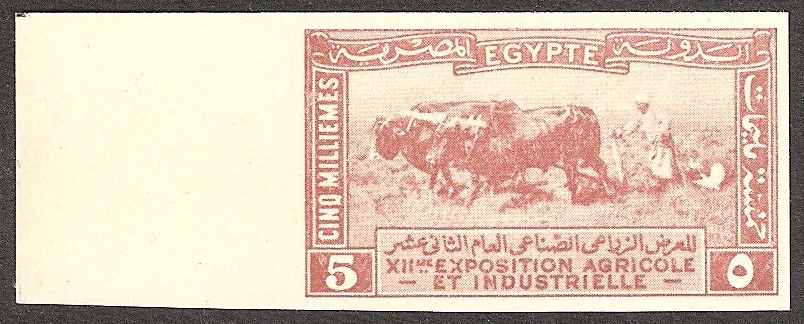
\includegraphics[scale=1.1]{./graphics/EG/SG126-cancelled} 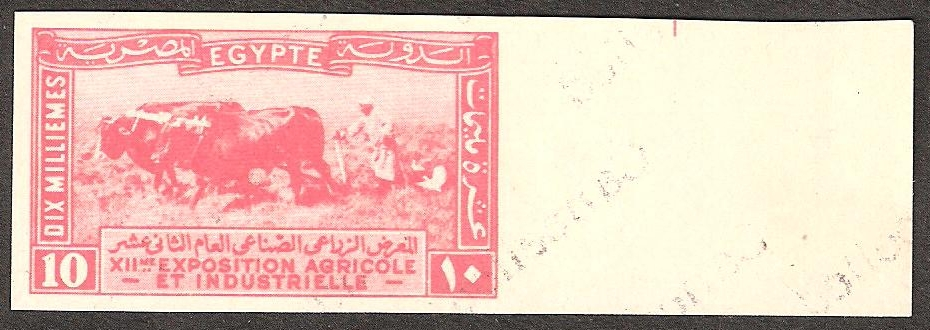
\includegraphics[scale=1.1]{./graphics/EG/SG127-cancelled}}

\bigskip
\hbox{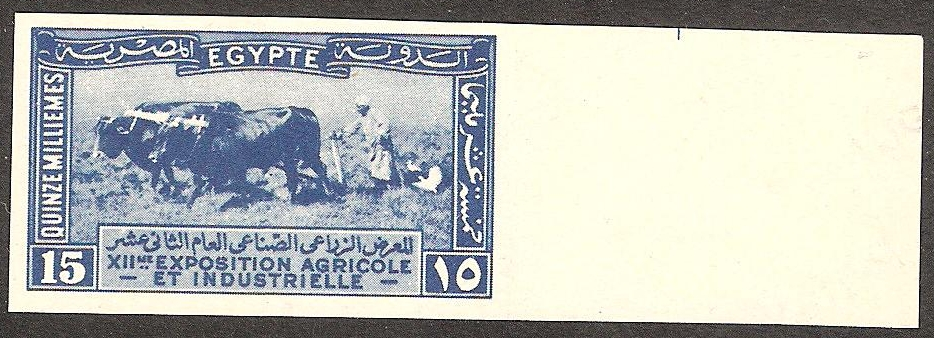
\includegraphics[scale=1.1]{./graphics/EG/SG128-cancelled}  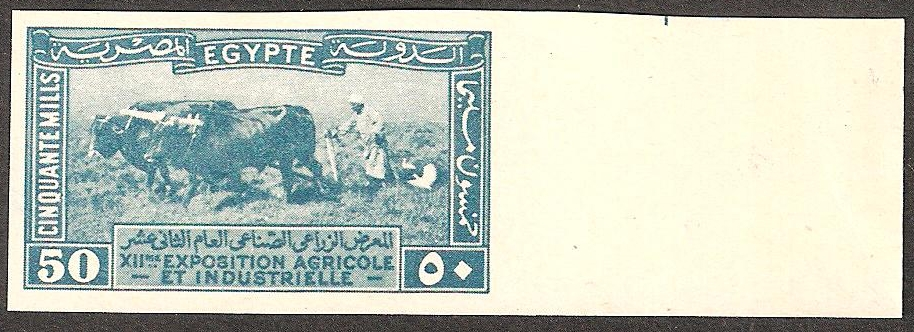
\includegraphics[scale=1.1]{./graphics/EG/SG129-cancelled}}
\bigskip

\hbox{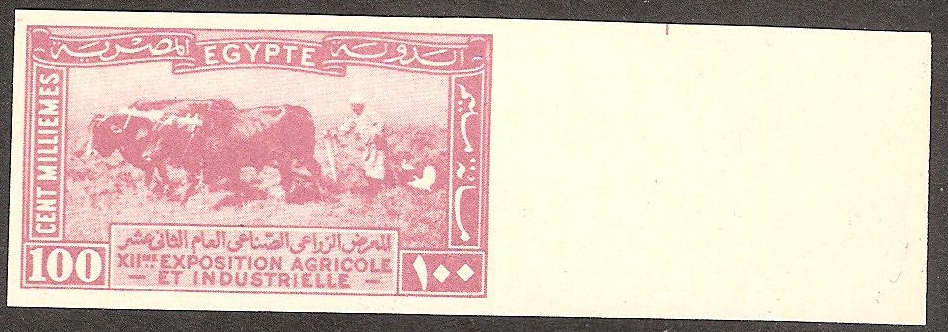
\includegraphics[scale=1.1]{./graphics/EG/SG130-cancelled} 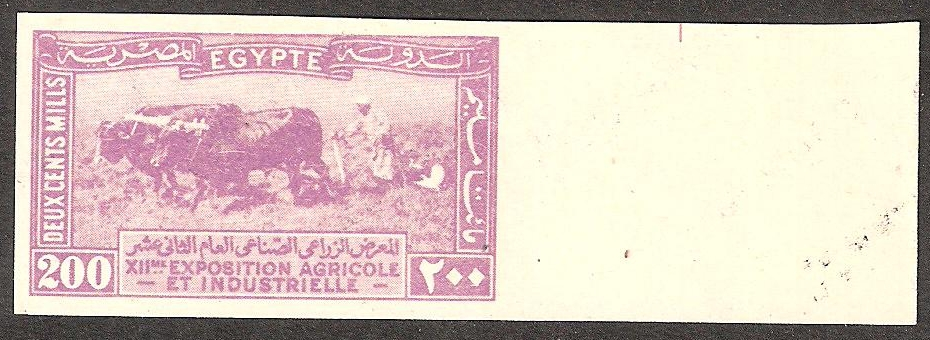
\includegraphics[scale=1.1]{./graphics/EG/SG131-cancelled}}
\bigskip
\end{fullwidth}
1926 12th Agricultural \& Industrial Exhibition set with cancelled on reverse 126-31 600 (NP C7b-12b) Feldman April 2008

The paper used for these 'cancelled' stamps was not treated very well and impressions of 'cancelled' can be found on the actual face of the stamps. Most amazing there is one full imprint on one of the stamps illustrated on the above set as shown below:

\begin{center}
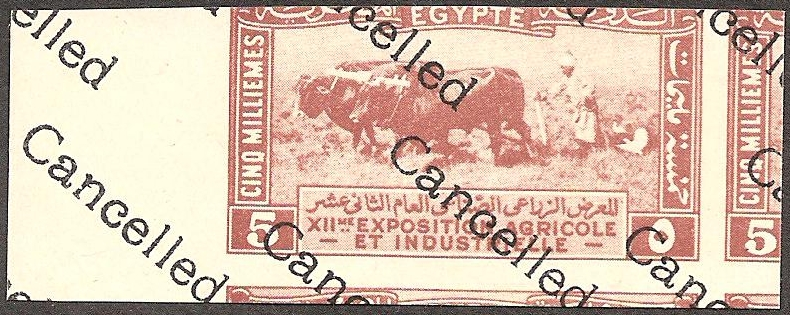
\includegraphics[scale=1.3]{./graphics/EG/SG126-cancelled-back}
\end{center}

The stamps exist both imperforate as well as having oblique perforations

\begin{center}
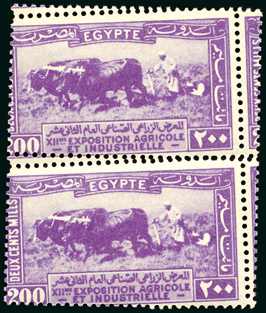
\includegraphics[scale=0.8]{./graphics/EG/SG131-oblique}
\end{center}
\medskip

1926 12th Agricultural Exhibition set of six in vert. pairs with oblique perfs, mint nh, a few very minor gum defects, fine (NP \$750) \euro300

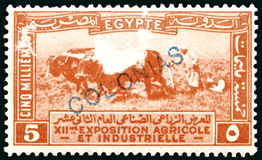
\includegraphics[scale=0.8]{./graphics/EG/SG126-colonias} 
\smallskip

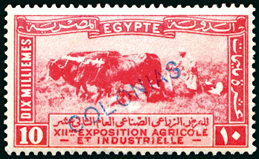
\includegraphics[scale=0.8]{./graphics/EG/SG127-colonias}
\smallskip

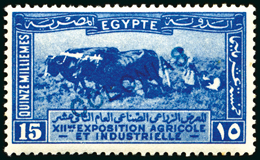
\includegraphics[scale=0.8]{./graphics/EG/SG128-colonias} 
\smallskip

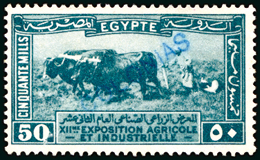
\includegraphics[scale=0.8]{./graphics/EG/SG129-colonias}
\smallskip

%\includegraphics[scale=0.8]{./graphics/EG/SG130-colonias}
%\smallskip

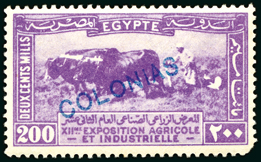
\includegraphics[scale=0.8]{./graphics/EG/SG131-colonias}
\smallskip


1926 12th Agricultural Exhibition set of six with \texttt{COLONIAS} hs, mint nh (50m no gum), 5m and 100m have surface scuffs, 200m bunt corner, the hs was applied to specimen stamps by the Portuguese postal authorites, the stamps are usually faulty, a scarce set \euro200

Auktionshaus Schlegel - Auction \#8, March 17-19, 2011


\newpage
\section{1933 Railway Congress}


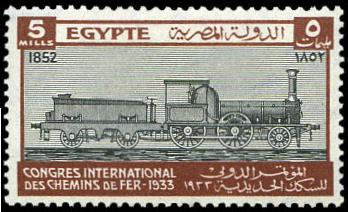
\includegraphics[width=0.43\textwidth]{./graphics/EG/Scott-168} 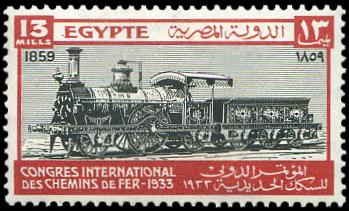
\includegraphics[width=0.43\textwidth]{./graphics/EG/Scott-169}
\medskip

\noindent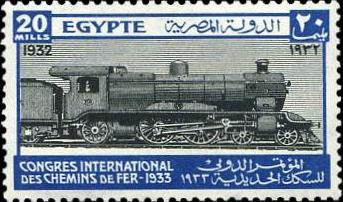
\includegraphics[width=0.43\textwidth]{./graphics/EG/Scott-170} 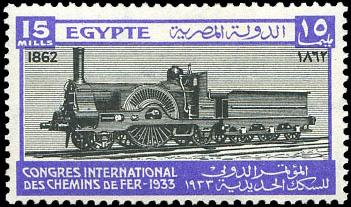
\includegraphics[width=0.43\textwidth]{./graphics/EG/Scott-171}
\vspace{0pt}
\index{1933!Railway Congress}
%%% Typeset side by side
%%% This needs some tuning
%\fbox{%
%\begin{minipage}[t]{16.5cm}
%\vspace{0pt}
%\begin{minipage}[t]{10.2cm}
%\vspace{0pt}
%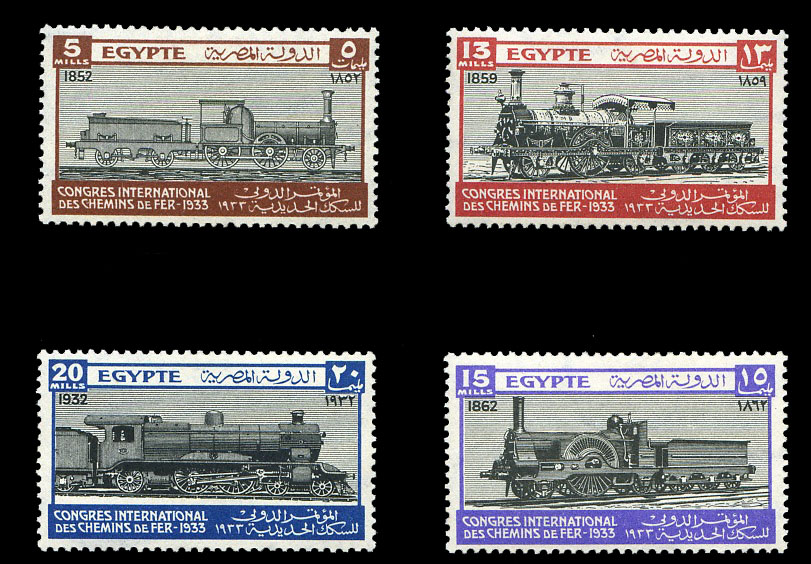
\includegraphics[width=\textwidth]{./graphics/EG/railway-set}
%\end{minipage}
%\hfill
%\begin{minipage}[t]{5.3cm}
%\vspace{0pt}
%\small
%1933 International Railroad Congress, set of four, hinged Scott 168-171
%\$55.00
%\end{minipage}
%\end{minipage}
%}
\bigskip
\begin{center}
\includegraphics[width=0.43\textwidth]{./graphics/EG/SG189-cancelled} \includegraphics[width=0.43\textwidth]{./graphics/EG/SG190-cancelled}
\medskip

\noindent\includegraphics[width=0.43\textwidth]{./graphics/EG/SG191-cancelled} 
\end{center}
1933 Railway Congress set of four imperf. with "CANCELLED" on reverse, very fine and scarce (NP \$700) \euro300
\bigskip

\marginpar{\RaggedRight \small 1933 Railway Congress set of four with oblique perfs, mint nh, very fine (NP \$500) Estimate \euro200}
\fbox{
\begin{minipage}{10.2cm}
\begin{center}
\vspace{0pt}
\includegraphics[width=0.43\textwidth]{./graphics/EG/SG189-oblique} \includegraphics[width=0.43\textwidth]{./graphics/EG/SG190-oblique}
\medskip

\noindent\includegraphics[width=0.73\textwidth]{./graphics/EG/SG191-oblique} 
\end{center}
\end{minipage}
}


\vspace{0pt}
\begin{tabular}{llp{3cm}l}
\toprule
Scott &date &description &value\\
\midrule
168   &1933 &5m black and brown locomotive no. 1 185 &5m\\
168   &1933 &5m black and brown locomotive no. 1 185 &5m\\
168   &1933 &5m black and brown locomotive no. 1 185 &5m\\
168   &1933 &5m black and brown locomotive no. 1 185 &5m\\
\midrule
\multicolumn{4}{l}{Scott Cat. Val. um \$70}\\
\multicolumn{4}{l}{Scott Cat. Val. mm \$70}\\
\bottomrule
\end{tabular}


\newpage

\section{1934 UPU Congress}
The 1934 UPU Congress gave Egypt their first commemorative set that had two high values included.

\medskip
\includegraphics[width=\textwidth]{./graphics/EG/UPU-cover}

1934 (March 31): UPU imprinted cover for CONGRESS in Cairo with special stationery insert in green, cover franked by UPU issue 20m. blue tied by special CONGRESS datestamps (two different) in blue.\euro55
\bigskip

%% Typeset side by side
%% This needs some tuning
\fbox{%
\begin{minipage}[t]{16.5cm}
\vspace{0pt}
\begin{minipage}[t]{10.2cm}
\vspace{0pt}
\includegraphics[width=\textwidth]{./graphics/EG/UPU-set}
\end{minipage}
\hfill
\begin{minipage}[t]{5.3cm}
\vspace{0pt}
\small
1934 UPU CONGRESS set 1m-\pounds1. VF fresh MLH. SG 219-32 cat \pounds750. Key set! (14) (P) Estimate A\$550
\end{minipage}
\end{minipage}
}




\section{1937 Prince}

\printph{EG}{PH778}

\printph{EG}{PH779}


\printph[1.39]{EG}{PH780}






\chapter{1942 Millenium of Al-Azhar Mosque}
\normalsize
\index{1942!Al-Azhar University, unissued}

When King Farouk's collection was sold at auction a number of surprises came. One was the unissued Al-Azhar University, stamps. Apparently only 102 of each value were printed and hence are quite rare.

The 1942 unissued Al-Azhar University set is made up of three values; 6m green, 15m dull purple and 20m gray, without the red overprint applied when the set was later released. Only 102 of each value were printed and discovered during the King Farouk auction.

\bigskip
\begin{center}
\includegraphics[width=0.43\textwidth]{./graphics/EG/al-azhar-6mils} \includegraphics[width=0.43\textwidth]{./graphics/EG/al-azhar-15mils}
\medskip

\noindent\includegraphics[width=0.43\textwidth]{./graphics/EG/al-azhar-20mills} 
\end{center}

\bigskip
\begin{center}
\includegraphics[width=0.63\textwidth]{./graphics/EG/al-azhar-6mils-oblique} 
\medskip

\includegraphics[width=0.43\textwidth]{./graphics/EG/al-azhar-15mils-oblique} \includegraphics[width=0.43\textwidth]{./graphics/EG/al-azhar-20mills-oblique} 
\end{center}

1942 Al-Azhar University (unissued) set of three with oblique perfs, mint nh, very fine and scarce, only 100 sets printed (NP 87b-90b, \$1'000)

Al-Azhar University is an educational institute in Cairo, Egypt. Founded in 970\~972 as a madrasa, it is the chief centre of Arabic literature and Sunni Islamic learning in the world.1 It is the oldest degree-granting university in Egypt after Cairo University. In 1961 non-religious subjects were added to its curriculum.2

It is associated with Al-Azhar Mosque in Islamic Cairo. The university's mission includes the propagation of Islamic religion and culture. To this end, its Islamic scholars (ulamas) render edicts (fatwas) on disputes submitted to them from all over the Sunni Islamic world regarding proper conduct for Muslim individuals and societies. Al-Azhar also trains Egyptian government appointed preachers in proselytization (da'wa).

Its library is considered second in importance in Egypt only to the Egyptian National Library and Archives. In May 2005, Al-Azhar in partnership with a Dubai information technology enterprise, ITEP launched the H.H. Sheikh Mohammed Bin Rashid Al Maktoum Project to Preserve Al Azhar Scripts and Publish Them Online (the ``Al-Azhar Online Project'') with the mission of eventually providing online access to the library's entire rare manuscripts collection (comprising about seven million pages).










\chapter{Consular Post Offices}\euro600

\normalsize

The special situation of Egypt as a nominal province of the Ottoman Empire and the special dispensations allowed to European citizens under the Capitulations meant that six foreign nations were allowed to operate national post offices in Egypt via their consulates. These were initially established in Alexandria and Suez, as the main ports at the time, and where most Europeans lived or conducted business. Later further offices were opened in Cairo and Port Said as their importance grew. 

These offices gave nationals of the respective countries the facility to send mail from Egypt to any destination within the foreign country served by its own mail routes. They operated with almost complete autonomy outside the Egyptian postal services and used their own national stamps and their own carriers for the transport of mail to and from Egypt. Incoming mails were delivered to the consulate and had to be collected by the addressee from the premises, while outgoing mail had to be franked with the stamps of the nationality of the shipping line. Mail could be sent from within Egypt to the consular post office by payment of the local Egyptian postage. After the introduction of Egyptian stamps in 1866 this led to some letters bearing stamps of both Egypt and of the country of destination. These fascinating "mixed frankings" are much sought-after and command a good premium. 

The foreign consular offices were established and operated as follows: France 1837-1931; Greece 1833-1881; Austria 1837-1874; Russia 1857-1875; Britain 1839-1878; Italy 1863-1884. In most cases the offices did not far outlast the first Universal Postal Union convention signed on 9 October 1874, which allowed postage to be paid in Egyptian stamps from anywhere within Egypt to within UPU signatory countries. Some foreign offices, however, continued to operate for the next decade, and the French Post Office hung on tenaciously up to April 1931. 

%%%%%%%%%%%%%%%%%%%%%%%%%%%%%%%%%%%%%%%%%%%%%%%%%%%%%%%%%%%%%%%%%%%%%%
%                   SUEZ
%
%%%%%%%%%%%%%%%%%%%%%%%%%%%%%%%%%%%%%%%%%%%%%%%%%%%%%%%%%%%%%%%%%%%%%%

\additem{EG}{PH20160}%
{The Famous Jean Boulad Study collection

Exhibition collection of mint Suez issues neatly mounted, illustrated and written up on 52 album pages (SG £73'880+)

- 1c black, type I with 18 positioned singles, type II with 23 positioned singles, type III with 21 positioned singles, type IV with 23 positioned singles, plus multiples incl. two pairs, block of four \& six (99) 

- 5c green, type I with 29 positioned singles, type II with 31 positioned singles, type III with 27 positioned singles, type IV with 28 positioned singles, plus multiples incl. three pairs, four blocks of four \& four blocks of six, five with "Lacroix Frères" watermark (166)

- 20c blue, complete reconstructed sheet of 120, study of 23 shades from light to dark blue, plus double impression, plus multiples incl. four pairs, one block of three, five blocks of four \& four blocks of six, sixteen with "Lacroix Frères" watermark (226)

- 40c pink, type I with 21 positioned singles, type II with 26 positioned singles, type III with 24 positioned singles, type IV with 25 positioned singles, plus multiples incl. two pairs, two blocks of four & two blocks of six, single \& marginal block of 18 with "Lacroix Frères" watermark (139)

A unique opportunity

Estimate: € 15'000 - € 20'000
}
{1854}%4
{EG/suez-1c}%5
{}%ex
{}
{}%
{}

\additem{EG}{PH20160a}%
{5c green, type I with 29 positioned singles, type II with 31 positioned singles, type III with 27 positioned singles, type IV with 28 positioned singles, plus multiples incl. three pairs, four blocks of four \& four blocks of six, five with "Lacroix Frères" watermark (166)
}
{1854}%4
{EG/suez-5c}%5
{}%ex
{}
{}%
{}

\additem{EG}{PH20160b}%
{ 20c blue, complete reconstructed sheet of 120, study of 23 shades from light to dark blue, plus double impression, plus multiples incl. four pairs, one block of three, five blocks of four \& four blocks of six, sixteen with "Lacroix Frères" watermark (226)
}
{1854}%4
{EG/suez-20c}%5
{}%ex
{}
{}%
{}

\additem{EG}{PH20161}%
{One of only 4 known covers from Kantara

1868 (Aug 15) Envelope from Kantara to Port Said, with four 5c green cancelled with pen manuscript (as were all from Kantara), paying the single rate, reverse with French PO Port Said pearl cds and signed by Ap. N. Gennaropoulo, incl. original letter datelined "Kantara, le 15 Aout, 1868," minor soiling.

One of only 21 known covers with a Suez Canal Company franking, of which only four were sent from Kantara. Illustrated on pg. 93 of "The Private Ship Letters of the World" by Ringström and Tester. A fantastic exhibition item.

Certification: RPS (2007), Holcombe (1991)

Provenance: Royal Collection, Antonini, Chiangir

Estimate: € 20'000 - € 30'000

}
{1854}%4
{EG/20161}%5
{}%ex
{}
{}%
{}

\additem{EG}{PH20162}%
{
1868 (Aug 12) Entire from Port Said to Kantara, with 20c blue tied by French "5129" lozenge of dots, paying single rate, reverse signed by Ap. N. Gennaropoulo, some minor cover faults.

One of only 12 covers sent from Port Said. Illustrated on pg. 87 of "The Private Ship Letters of the World" by Ringström and Tester. A fine addition to a top exhibition collection.

Certification: RPS (1947), A. Diena (1976), Bolaffi (1977) and E. Diena (1983), signed Calves on front, Robson Lowe on reverse

Provenance: Chafter

Estimate: € 8'000 - € 12'00
Realised:
18'000 EUR
}
{1854}%4
{EG/20162}%5
{}%ex
{}
{}%
{}


\additem{EG}{PH20163}%
{1c Black with very good to huge margins and neat French "5129" lozenge cancel, small thin spot, fine appearance, only four known examples with the Port Said cancel according to Ringström and Tester, cert. RPS (1971) (SG £1'000)
The Fikry Collection of The Suez Canal Zone. 1868 Suez Canal Company issue (SG 1-4)
Estimate: 400 EUR
Price realised: 1'800 EUR on Thu 19th May 2011 Feldmans
}
{1854}%4
{EG/20163}%5
{}%ex
{}
{}%
{}


\additem{EG}{PH20164}%
{5c Green with very good margins and French "5129" lozenge cancel, very fine, only three known examples with the Port Said cancel according to Ringström and Tester (one of which is in the Tapling collection in the British Library), cert. RPS (1971) (SG £500)Estimate: 300 EUR
Price realised: 1'800 EUR on Thu 19th May 2011
}
{1854}%4
{EG/20164}%5
{}%ex
{}
{}%
{}









\chapter{Suez}
\printph[1.4]{EG}{PH781}

\printph{EG}{PH20160}

\printph{EG}{PH20160a}

\printph{EG}{PH20160b}

\newpage

%Cover Suez
\printside{EG}{PH20161}

\printside{EG}{PH20162}

\newpage
\printside[0.35]{EG}{PH20163}

\printside[0.35]{EG}{PH20164}


\chapter{French}
\printph{EG}{PH782}

\printph{EG}{PH783}

\printph{EG}{PH784}

\printph{EG}{PH785}

\printph{EG}{PH786}

\printph{EG}{PH20226}


\printph{EG}{PH787}

\printph{EG}{PH788}

\printph{EG}{PH789}

\printph{EG}{PH790}



\printph{EG}{PH791}

\printph{EG}{PH792}

\printph{EG}{PH793}

\printph{EG}{PH794}

\printph{EG}{PH795}


\printph{EG}{PH796}

\printph{EG}{PH797}

\printph{EG}{PH798}

\printph{EG}{PH799}

\printph{EG}{PH800}

\printph{EG}{PH801}

\printph{EG}{PH802}

\printph{EG}{PH803}

\printph{EG}{PH804}

\printph{EG}{PH805}


\chapter{Greek Post office}
\printph{EG}{PH806}

%% Syros
\printph{EG}{PH807}

\printph{EG}{PH20058}


\printph{EG}{PH808}

\chapter{Italian Post Office Alexandria}
\printph{EG}{PH809}

\printph{EG}{PH810}

\newpage
%% ballon de monte
\chapter{Airmails}

The Gold Medal collection of Dr. Adel Farid ``Egyptian Airmails'' had a Ballon de Monte cover addressed to Cairo and this is perhaps the earliest item associated with aviation and Egypt. Of course it never travelled by ballon to Alexandia, but nevertheless it is an interesting cover\sidenote{Sold by Corinphila in December 2010.}.
\printside{EG}{PH811}

\newpage

\printside[0.5]{EG}{PH812}

\printside[0.7]{EG}{PH813}


\newpage

\printside{EG}{PH814}

\printside{EG}{PH815}

\newpage


\printside{EG}{PH816}

\printside{EG}{PH817}

\newpage

\printside{EG}{PH818}

\normalsize

\begin{marginfigure}
\includegraphics[width=\textwidth]{./graphics/EG/SirGeoffreySalmond}
\caption{Air Vice-Marshal Sir Geoffrey Salmond}
\end{marginfigure}
Air Chief Marshal Sir William Geoffrey Hanson Salmond KCB, KCMG, DSO (19 August 1878[1] - 27 April 1933), commonly known as Sir Geoffrey Salmond, was a senior commander in the Royal Flying Corps during World War I. Remaining in the Royal Air Force after the War, he held senior appointments in the Middle East, Great Britain and India. In 1933 Salmond served as Chief of the Air Staff for several weeks before his death from cancer.

On 18 February 1913 Salmond was awarded Royal Aero Club Aviator's Certificate no. 421, after which. on 17 April 1913, he joined the reserve of the Royal Flying Corps (RFC),[4] although he continued to serve in the regular army. Following staff work in military aeronautics, he went on to take up the post of Officer Commanding, No. 1 Squadron RFC.[4] In the First World War the squadron operated over the Western Front and Salmond and his squadron took part in the Battle of Neuve Chapelle, including the Battle of Hill 60 and the Battle of Aubers Ridge.[4]

In 1916 he was sent to command the 5th Wing, RFC,[4] in Egypt, and in July, 1916, he was promoted to temporary Brigadier-General and given command of the RFC in the Middle East,[4] a post which he held with brief intervals, until the end of 1921. The DSO was conferred on him in the London Gazette of 3 March 1917,[4] "for conspicuous ability and devotion to duty when personally directing the work of the Royal Flying Corps during the action.[2] The striking success attained was largely due to his magnificent personal example." The action referred to was during the operations in Sinai at the end of 1916.[2] In this command he was responsible for providing air cooperation for General Jan Smuts's force in East Africa,[3] for the forces in Salonika and Mesopotamia, for Allenby's conquest of Palestine, and for the RFC in India.[3]

While holding the command of the Middle East, he had laid out an airway from Cairo to South Africa,[2] clearing a chain of aerodromes in Central Africa. His idea was to send a demonstration flight or flights of RAF aircraft across Africa, thus providing the link of which Cecil Rhodes had dreamed in a Cape-to-Cairo railway.[3] Salmond contemplated flights by both landplane and flying-boat. He was not destined to put his idea into execution, though his airway was used by Sir Pierre van Ryneveld and Sir Christopher Brand on their first flight to South Africa.[3]
\newpage

\printside{EG}{PH819}

\printside{EG}{PH820}
\newpage

\printside{EG}{PH821}

\newpage

\printside{EG}{PH822}


\newpage
\printside{EG}{PH823}

\newpage
\printside[0.9]{EG}{PH824}

\printside[0.75]{EG}{PH825}

\newpage

\printside{EG}{PH826}
\newpage

\section{Insufficient Postage Payment}
\printside{EG}{PH827}
\newpage

%%% 840
\printside{EG}{PH840}

\printside{EG}{PH841}

\newpage

\printph{EG}{PH842}



\printph{EG}{PH843}


\printph{EG}{PH844}


\printph{EG}{PH845}

\printph{EG}{PH846}

\printph{EG}{PH847}

\printph{EG}{PH848}

\printph{EG}{PH849}


\printph{EG}{PH850}


\printph{EG}{PH851}

\printph{EG}{PH852}

\printph{EG}{PH853}

\pagebreak
\printph{EG}{PH854}

\printph{EG}{PH855}

\printph{EG}{PH856}

\printph{EG}{PH857}

\printph{EG}{PH858}

\printph{EG}{PH859}

\printph{EG}{PH860}

\printph{EG}{PH861}

\printph{EG}{PH862}

\printph{EG}{PH863}

\printph{EG}{PH864}

\printph{EG}{PH865}

\printph{EG}{PH866}

\printph{EG}{PH867}

\printph{EG}{PH868}

\printph{EG}{PH869}

\printph{EG}{PH870}


\printph{EG}{PH871}

\printph{EG}{PH872}

\printph{EG}{PH873}


%\printph{EG}{PH874}

\printph{EG}{PH875}

\printph{EG}{PH876}

\printph{EG}{PH877}

\printph{EG}{PH878}

\printph{EG}{PH879}


\printph{EG}{PH880}

\printph{EG}{PH881}

\printph{EG}{PH882}

\printph{EG}{PH883}

\printph{EG}{PH884}

\printph{EG}{PH885}

\printph{EG}{PH886}

\printph{EG}{PH887}

\printph{EG}{PH888}

\printph{EG}{PH889}

\printph{EG}{PH890}


\printph{EG}{PH891}

\printph{EG}{PH892}

\printph{EG}{PH893}

%\printph{EG}{PH894}

1931 (April 6): Surcharged 50 m. on 27 m. and 100 m. on 27 m. the mint blocks of ten of each value from base of sheet with corner Control numbers "A29" on each. Very rare in multiples of this size: only 10 sets of the issue could be purchased by any one customer from the four Post Offices where the issue was distributed, thus these are the largest multiples that should exist - also showing varieties spaced '5 and 0' on pos. 47, and dot under arabic date on the 100 m. value (pos. 46). Fresh and fine, large part to unmounted original gum Gi = \pounds{840}. 

Note: Of 22'050 sets printed, 2'950 were destroyed as the surcharges were poor, 1'600 were sent to the UPU in Berne, 2'000 sets were retained by the Govt., 8'000 sets were used on mail, 1'000 sets were cancelled to order. This left approximately 9'450 sets available to the public.(500/2600)

\newpage
%% ZEPPELIN
\chapter{Zeppelin Flights}
\printside{EG}{PH895}

\printside{EG}{PH896}

\newpage

\printside{EG}{PH897}

\printside{EG}{PH898}

\newpage

%\printside{EG}{PH899}

\printside{EG}{PH900}

\newpage
\printside{EG}{PH901}

\printside{EG}{PH902}

\newpage

\printside{EG}{PH903}

\printside{EG}{PH904}

\newpage

\printside{EG}{PH905}

\printside{EG}{PH906}

\newpage

\printside{EG}{PH907}

\printside{EG}{PH908}

\newpage

\printside{EG}{PH909}

\printside{EG}{PH910}

\newpage



\printside{EG}{PH911}

\printside{EG}{PH912}

\newpage

\printside{EG}{PH913}

\printside{EG}{PH914}

\newpage

\printside{EG}{PH915}

\printside{EG}{PH916}

\newpage
\printside{EG}{PH917}


\printside{EG}{PH918}

\newpage
\printside{EG}{PH919}


\printside{EG}{PH920}










%\printindex
\end{document}















